% !TEX TS-program = xelatex
% !TeX program = xelatex
% !TEX encoding = UTF-8
% !TEX spellcheck = en_US

\documentclass{KBook}

%To prevent other chapters from creating a new document
\let\wholebook=\relax

%The calls (includes) for other packages are in a separate file
\input{calls}


%opening
\title{Natural Language Processing}

\author{Abdelkrime Aries}
\cover{../img/misc/cover.jpg}
\license{../img/licence/cc-by.png}

\publisher{../img/misc/esi-logo.png}

%\setplainversion

\begin{document}
	
\maketitle

\frontmatter

\addcontentsline{toc}{chapter}{General information}

\shipout\null %blank page after the title 

\input{a.01.copyright}

%\input{a.02.preface}

\addcontentsline{toc}{chapter}{Contents and lists}

\kodetoc

\kodelof

\kodelot

\kodeloa

\kodeabbrev

\mainmatter

%\acolor{everything}{olivegreen} 

\input{b.00.intro}

\input{b.01.introNLP}

% !TEX TS-program = xelatex
% !TeX program = xelatex
% !TEX encoding = UTF-8
% !TEX spellcheck = en_US

%=====================================================================
\ifx\wholebook\relax\else
	\documentclass{KBook}
	\input{calls}
	\begin{document}
		\mainmatter
	
\fi
%=====================================================================
\changegraphpath{../img/ml4nlp/}

\chapter{Machine learning for NLP}

\begin{introduction}[N\textcolor{white}{A}T. LANG. PROC.]
	
	\lettrine{A}{lmost} all NLP tasks need machine learning to be achieved or can used it to enhance results. 
	
\end{introduction}

\begin{itemize}
	\item \optword{NB}: Naive Bayes
	\item \optword{LR}: Logistic regression
	\item \optword{SVM}: Support-Vector Machine
	\item \optword{NN}: Neural Network
	\item \optword{FFN}: Feed Forward Network
	\begin{itemize}
		\item \optword{MLP}: Multi-Layer Perceptron
		\item \optword{CNN}: Convolutional Neural Network
	\end{itemize}
	\item \optword{RNN}: Recurrent Neural Network
	\item \optword{HMM}: Hidden Markov Model
	\item \optword{MEMM}: Maximum-Entropy Markov Model
	\item \optword{CRF}: Conditional Random Field
\end{itemize}

\begin{tabular}{p{.12\textwidth}lp{.37\textwidth}lp{.38\textwidth}}
	
	&& Generative && Discriminative \\
	
	&&&&\\
	
	Text && NB && LR, SVM, MLP, RNN, CNN \\
	
	&&&&\\
	
	Sequence && HMM  && MEMM, CRF, RNN \\
	
\end{tabular}



\begin{itemize}
	\item \optword{Generative model}: a model that learns to generate features given a class:
	\[\hat{Y} = \arg\max_k P(Y_k) P(X | Y_k)\]
	
	\item \optword{Discriminative model}: a model that learns to estimate a class given some features: 
	\[\hat{Y} = \arg\max_k P(Y_k | X)\]
\end{itemize}


%===================================================================================
\section{Machine learning}
%===================================================================================

%\begin{frame}
%	\frametitle{ML for NLP}
%	\framesubtitle{\insertsection}
	
	\begin{itemize}
		\item This section is a review of ML algorithms
		\item Traditional ML algorithms: LR, SVM, DT, NB
		\begin{itemize}
			\item Text features are engineered manually
		\end{itemize}
		\item MLP (Multi-Layer Perceptron)
		\begin{itemize}
			\item Text features can be learned/enhanced automatically
			\item The terminology is wrongly used to refer to Fully connected feed-forward neural networks with at least three layers
		\end{itemize}
		\item CNN (Convolutional Neural Network)
		\begin{itemize}
			\item Extracting relations between consecutive units
		\end{itemize}
		\item RNN (Recurrent Neural Network)
		\begin{itemize}
			\item Temporal dependent units processing
		\end{itemize}
	\end{itemize}
	

Example (Simple Perceptron for binary logical functions)
	
	\begin{minipage}{0.30\textwidth} 
		\hgraphpage{perceptron.pdf}
	\end{minipage}
	%
	\begin{minipage}{0.59\textwidth}
		\scriptsize
		\begin{itemize}
			\item $ z^{(i)} = x_1^{(i)} w_1 + x_2^{(i)} w_2 + b $
			\item $ \hat{y}^{(i)} = \phi(z^{(i)}) = \begin{cases}
				1 & \text{if } z^{(i)} \ge 0 \\
				0 & \text{otherwise}
			\end{cases} $
			\item $ w_j = w_j + \nabla w_j$ where $ \nabla w_j = \frac{1}{M}\sum_{i=0}^{M} (y^{(i)} - \hat{y}^{(i)}) * x_j^{(i)} $
		\end{itemize}
	\end{minipage}
	
	\vfill
	
	Training a Perceptron for AND function
		\begin{minipage}{0.2\textwidth} 
			\scriptsize
			\begin{tabular}{|c|c|c|}
				\hline
				x\textsubscript{1} & x\textsubscript{2} & y \\
				\hline
				0 & 0 & 0  \\
				\hline
				0 & 1 & 0 \\
				\hline
				1 & 0 & 0 \\
				\hline
				1 & 1 & 1 \\
				\hline
			\end{tabular}
		\end{minipage}
		%
		\begin{minipage}{0.79\textwidth}
			\scriptsize
			\begin{itemize}
				\item Initially, $ W = [w_1, w_2, b] = [0, 0, 0] $.
				
				\item It1: $ Z = \hat{Y} = [0, 0, 0, 0] $, 
				$ \nabla W = [\frac{1}{4}, \frac{1}{4}, \frac{1}{4}] $, 
				$ W = [\frac{1}{4}, \frac{1}{4}, \frac{1}{4}] $.
				
				\item It2: $ Z = [\frac{1}{4}, \frac{2}{4}, \frac{2}{4}, \frac{3}{4}] $, 
				$ \hat{Y} = [1, 1, 1, 1] $, 
				$ \nabla W = [\frac{-1}{4}, \frac{-1}{4}, \frac{-3}{4}] $,
				$ W = [0, 0, \frac{-1}{2}] $.
				
				\item It3: $ Z = [\frac{-1}{2}, \frac{-1}{2}, \frac{-1}{2}, \frac{-1}{2}] $, 
				$ \hat{Y} = [1, 1, 1, 1] $, 
				$ \nabla W = [\frac{1}{4}, \frac{1}{4}, \frac{1}{4}] $,
				$ W = [\frac{1}{4}, \frac{1}{4}, \frac{-1}{4}] $.
				
				\item It4: $ Z = [\frac{-1}{4}, 0, 0, \frac{1}{4}] $, 
				$ \hat{Y} = Y = [0, 0, 0, 1] $ (STOP)
			\end{itemize}
		\end{minipage}


\subsection{Traditional ML}

	
	\begin{itemize}
		%			\item Features are engineered manually 
		\item The classification model stores some parameters $\theta$
		\begin{itemize}
			\item They are used by an inference function $ f $ to find the perfect class.
			\item They can be considered to be some rules on the input to find the output.
			\item Eg. \expword{IF weather = warm THEN play}
		\end{itemize}
		\item These parameters are trained using an algorithm based on some data
		\begin{itemize}
			\item They are tuned so the model find the exact output of the data
		\end{itemize}
		\item The data is a table of samples, features and class
		\begin{itemize}
			\item Let's consider $ M $ samples (rows) and $ N $ features (columns)
			\item $ X[M, N] $ is the input
			\item $ Y[M] $ is the output
		\end{itemize}
		\item In summary, to infer a class $ \hat{y} $ of a sample $ x $
		\[\hat{y} = f(x, \theta)\]
	\end{itemize}
	
	
	Linear Regression
	
	\begin{minipage}{0.62\textwidth} 
		\begin{itemize}
			\item \textbf{GOAL}: Try to estimate a value $ y $ based on some features $ x $
			\item \textbf{Estimation}: $ \hat{y} = \theta_0 + \sum_{j=1}^{N} \theta_j x_j $
			\item \textbf{Training}: Try to minimize a cost function $ J $
			\[J_\theta = \frac{1}{2M} \sum\limits_{i=1}^{M} (y^{(i)} - \hat{y}^{(i)})^2\]
			%				\item $J_\theta = \frac{1}{M} \sum\limits_{i=1}^{M} (y^{(i)} - \hat{y}^{(i)})^2$
			%				\item Eg. \expword{Houses prices based on their areas}
		\end{itemize}
	\end{minipage}
	\begin{minipage}{0.37\textwidth} 
		\hgraphpage{houses_LR.png}
	\end{minipage}
	
	\begin{itemize}
		
		\item Update each parameter $ \theta_j $ iteratively using a learning rate $ \alpha $
		\[\theta_j = \theta_j - \alpha \frac{\partial J_\theta}{\partial \theta_j}
		\hspace{1cm}
		\frac{\partial J_\theta}{\partial \theta_j} = \frac{1}{M} \sum\limits_{i=1}^{M} (\hat{y}^{(i)} - y^{(i)}) x_j
		\]
		\item The update is stopped when the cost is minimal
	\end{itemize}
	
	Linear Regression (Cost and parameters)
	
	\begin{minipage}{0.7\textwidth} 
		\begin{block}{Gradient descent}
			\begin{algorithm}[H]
				\KwData{$ X, Y, \alpha, T $}
				\KwResult{$ \theta $}
				initialize $ \theta $ ; $ t = 0 $\;
				calculate $ J $\;
				\While{$ t < T$ and $ J \ge tol $}{
					$ \theta = \theta - \alpha \Delta_\theta J(X, Y; \theta) $\;
					calculate $ J $\;
					t = t + 1 \;
				}
				%					\caption{Gradient descent}
			\end{algorithm}
		\end{block}
	\end{minipage}
	\begin{minipage}{0.29\textwidth} 
		\hgraphpage{J.pdf}
	\end{minipage}
	
	Binary Logistic Regression
	
	\begin{minipage}{0.5\textwidth} 
		\hgraphpage{LR_bin_arch.pdf}
	\end{minipage}
	\begin{minipage}{0.49\textwidth} 
		\hgraphpage{exp_binary.pdf}
	\end{minipage}
	
	Binary Logistic Regression (Formalism)
	
	\begin{minipage}{0.5\textwidth} 
		\begin{itemize}
			\item \textbf{GOAL}: Try to draw a decision line between two classes $ y \in \{0, 1\} $ based on some features $ x $
			\item \textbf{Estimation}: $ z = \theta_0 + \sum_{j=1}^{N} \theta_j x_j $
			$ h = \sigma(z) = \frac{1}{1 + e^{-z}}$, $ \hat{y} = (h \ge 0.5)$
		\end{itemize}
	\end{minipage}
	\begin{minipage}{0.49\textwidth} 
		\hgraphpage{grades_LR.png}
	\end{minipage}
	
	\begin{itemize}
		\item \textbf{Training}: Try to minimize a cost function $ J $
		\[J_\theta = \frac{-1}{M} \sum\limits_{i=1}^{M} y^{(i)} \log(h^{(i)}) + (1- y^{(i)}) \log(1 - h^{(i)})\]
		\item Update each parameter $ \theta_j $ iteratively using a learning rate $ \alpha $
		\[\theta_j = \theta_j - \alpha \frac{\partial J_\theta}{\partial \theta_j}
		\hspace{1cm}
		\frac{\partial J_\theta}{\partial \theta_j} = \frac{1}{M} \sum\limits_{i=1}^{M} (\hat{y}^{(i)} - y^{(i)}) x_j
		\]
		%			\item The update is stopped when the cost is minimal
	\end{itemize}
	
	Multinomial Logistic Regression
	
	\begin{minipage}{0.6\textwidth} 
		\hgraphpage{LR_multi_arch.pdf}
	\end{minipage}
	\begin{minipage}{0.39\textwidth} 
		\hgraphpage{exp_multiclass.pdf}
	\end{minipage}
	
	Multinomial Logistic Regression (Formalism)
	
	\begin{minipage}{0.7\textwidth} 
		\begin{itemize}
			\item \textbf{GOAL}: Try to draw decision lines between many classes $ y $ based on some features $ x $
			\item \textbf{Estimation}: $ z_l = \theta_{0l} + \sum_{j=1}^{N} \theta_{jl} x_j $
			$ h_l = Softmax(z_l) = \frac{e^{z_l}}{\sum_{k=1}^{L} e^{z_k}}$, $ \hat{y} = \arg\max_{l} h_l$
			\item \textbf{Also}: $ L $ binary logistic classifiers. 
			The probabilities are normalized: $ \sum_{l=1}^{L} p(c_l) = 1$.
			%				Each estimates a probability of a class $ c_l $.
			%				Then, these probabilities are normalized to have normalized probabilities $ \sum_{l=1}^{L} p(c_l) = 1$.
		\end{itemize}
	\end{minipage}
	\begin{minipage}{0.29\textwidth} 
		\hgraphpage{multi_LR.pdf}
	\end{minipage}
	
	\begin{itemize}
		\item \textbf{Training}: Try to minimize a cost function $ J $
		\[J_\theta = \frac{-1}{M} \sum\limits_{i=1}^{M} \sum_{k=1}^{L} h^{(i)}_k \log(h^{(i)}_k)
		\hspace{1cm}
		\frac{\partial J_\theta}{\partial \theta_{jl}} = \frac{1}{M} \sum\limits_{i=1}^{M} (h_l^{(i)} - y_l^{(i)}) x_j
		\]
	\end{itemize}
	
	Support-Vector Machine (Primal form)
	
	\begin{minipage}{0.75\textwidth} 
		\begin{itemize}
			\item \textbf{GOAL}: Try to draw a decision line between two classes $ y $ based on some features $ x $ like LR. But, in this case the margin between the two classes must be maximal.
			\item \textbf{Estimation}: $ z = b + \sum_{j=1}^{N} \theta_j x_j $, 
			$ \hat{y} = (z \ge 0.5)$
		\end{itemize}
	\end{minipage}
	\begin{minipage}{0.24\textwidth} 
		\hgraphpage{SVM_primal.pdf}
	\end{minipage}
	
	\begin{itemize}
		\item \textbf{Training}: Try to minimize a cost function $ J $, $ y \in \{-1, 1\} $
		\[J_\theta = \frac{1}{M} \left[ \frac{1}{2}||\theta||^2 + C \sum\limits_{i=1}^{M} \max (0, 1 - y^{(i)} z^{(i)}) \right]
		%			\hspace{1cm}
		%			\frac{\partial J_\theta}{\partial \theta_{jl}} = \frac{1}{M} \sum\limits_{i=1}^{M} (h_l^{(i)} - y_l^{(i)}) x_j
		\]
		
		\[\frac{\partial J_\theta}{\partial \theta_{j}} = \frac{1}{M} \left[ \theta_j + \sum\limits_{i=1}^{M} \begin{cases}
			0 & \text{if } y^{(i)} z^{(i)} \ge 1\\
			- C x^{(i)}_j y^{(i)} & \text{otherwise}  \\
		\end{cases} \right]
		\]
	\end{itemize}
	
	Support-Vector Machine (Dual form)
	
	\begin{minipage}{0.75\textwidth} 
		\begin{itemize}
			\item \textbf{GOAL}: The same as Primal form's, but a new sample is represented by its similarity to training samples
			\item \textbf{Estimation}: 
			\[\hat{y_t} = sign(\sum^M_{i=1} \alpha_i y^{(i)} K(x^{(i)}, x_t) - b)\]
		\end{itemize}
	\end{minipage}
	\begin{minipage}{0.24\textwidth} 
		\hgraphpage{SVM_dual.pdf}
	\end{minipage}
	
	
	\begin{itemize}
		\item \textbf{Training}: Try to minimize a cost function $ J $
		\[J_\alpha = \sum\limits_{i=1}^{M} \alpha_i - \frac{1}{2} \sum\limits_{i=1}^{M} \sum\limits_{j=1}^{M} \alpha_i \alpha_j y^{(i)} y^{(j)} K(x^{(i)}, x^{(j)})\]
		\item $\alpha$ and $ b $ are updated using an optimization algorithm like \keyword{Sequential minimal optimization}
	\end{itemize}
	
	Decision Trees
	
	Example of expected model
		\begin{minipage}{0.33\textwidth} 
			\tiny\bfseries
			\begin{tabular}{llllll}
					id & outlook & temp & humidity & windy & play \\
					01 & sunny & hot & high & false & no \\
					02 & sunny & hot & high & true & no \\
					03 & overcast & hot & high & false & yes \\
					04 & rainy & mild & high & false & yes \\
					05 & rainy & cool & normal & false & yes \\
					06 & rainy & cool & normal & true & no \\
					07 & overcast & cool & normal & true & yes \\
					08 & sunny & mild & high & false & no \\
					09 & sunny & cool & normal & false & yes \\
					10 & rainy & mild & normal & false & yes \\
					11 & sunny & mild & normal & true & yes \\
					12 & overcast & mild & high & true & yes \\
					13 & overcast & hot & normal & false & yes \\
					14 & rainy & mild & high & true & no \\
					%			\end{tabular}
			\end{tabular}
		\end{minipage}
		\begin{minipage}{0.25\textwidth} 
			\tiny\bfseries\itshape
			\textcolor{red}{if} outlook == '\textcolor{darkgreen}{sunny}':\\
			\hspace*{10pt}\textcolor{red}{if}  humidity == '\textcolor{darkgreen}{high}':\\
			\hspace*{20pt}\textcolor{red}{return}  '\textcolor{darkgreen}{no}'\\
			\hspace*{10pt}\textcolor{red}{else}: \textcolor{gray}{\# 'normal'}\\
			\hspace*{20pt}\textcolor{red}{return} '\textcolor{darkgreen}{yes}'\\
			\textcolor{red}{elif}  outlook == '\textcolor{darkgreen}{overcast}':\\
			\hspace*{10pt}\textcolor{red}{return} '\textcolor{darkgreen}{yes}'\\
			\textcolor{red}{else}: \textcolor{gray}{\# 'rainy'}\\
			\hspace*{10pt}\textcolor{red}{if not} windy:\\
			\hspace*{20pt}\textcolor{red}{return} '\textcolor{darkgreen}{yes}'\\
			\hspace*{10pt}\textcolor{red}{else}:\\
			\hspace*{20pt}\textcolor{red}{return} '\textcolor{darkgreen}{no}' 
		\end{minipage}
		\begin{minipage}{0.38\textwidth} 
			\hgraphpage{exp_DT.pdf}
		\end{minipage}
	
	\vspace{-6pt}
	\begin{itemize}
		\item \textbf{GOAL}: Create a tree by splitting the training data. The leafs must contain homogeneous samples (same class)
		\item \textbf{Estimation}: navigate the tree from the root till a leaf based on the sample's features
	\end{itemize}
	
	Decision Trees (Training)
	
	\begin{block}{Decision tree construction}
		\scriptsize
		\begin{algorithm}[H]
			\SetKwFunction{FConst}{build}
			\SetKwProg{Fn}{function}{}{end}
			
			\KwData{$ X, Y$}
			\KwResult{Decision tree's root node} 
			\Return \FConst{$X, Y$}\;
			
			\Fn{\FConst{$X', Y'$}}{
				n $\leftarrow$ new Node()\;
				\eIf{$Y'$ is homogeneous or stop criteria is reached}{
					$s.class \leftarrow \arg\max_{k}{|\{y \in Y' / y = k \}|}$ \tcp{$s$ is a leaf}
				}{
					determine the feature $j$ of $ X' $ which better divides $Y'$\;
					split $(X, Y)$ into $(X_1, Y_1), \ldots, (X_K, Y_K)$ based on the $ K $ values of $X'_j$\;
					$s.feature = j$\;
					\lForEach{$ k \in \{1, \ldots, K\}$}{
						%							$s_k \leftarrow Construction(X_{*,k}, Y_k) \in S$ $(s, s_k) \in A$ $val(s, s_k) = k$\;
						$ n.children[k] \leftarrow$ \FConst{$ X_k, Y_k $})
					}
				}
				
				\Return n\;
			}	
			
			%				\caption{Génération d'un arbre de décision (algorithme général)}
		\end{algorithm}
	\end{block}
	
	Decision Trees (ID3: Iterative Dichotomiser 3)
	
	\begin{itemize}
		\item \textbf{LEARN MORE}: \cite{1986-quinlan}
		\item Probability of a given value $ v $ belonging into a set $ S $
		\[p(v\in S) = \frac{|\{x / x\in S \text{ and } x = v\}|}{|S|}\]
		\item Entropy: uncertainty of a set $ S $ having a set $ V $ of unique values
		\[H(S) = - \sum\limits_{v \in V} p(v\in S) \log_2 p(v\in S)\]
		\item Information gain: difference in entropy from before to after the set $ S $ is split on an attribute $ A $ with $ V $ unique values.
		\[IG(Y, A) = H(Y) - \sum_{v \in V} p(v\in A) H(Y_{v\in A})\] 
	\end{itemize}
	
	\[H(Y) = 0 \Rightarrow\ Y \text{ is homogeneous} \hspace{1cm} j_{best} = \arg\max_j IG(Y, X_j)\]
	
	Decision Trees (ID3 - Example and application)
	\begin{enumerate}
		\item Create a node $ ROOT $
		\begin{itemize}\tiny\bfseries
			\item $ H(Y) = - p(yes \in Y) \log_2 p(yes\in Y) - p(no \in Y) \log_2 p(no\in Y)  $
			$ = -\frac{9}{14} \log_2 \frac{9}{14} - \frac{5}{14} \log_2 \frac{5}{14} \approx\ 0.94$ (not pure)
			%				\item $ IG(Y, outlook) = H(Y) - \sum_{v \in \{sunny, overcast, rainy\}} p(v\in A) H(Y_{v\in outlook}) $
			\item $ IG(Y, outlook) = 0.94 - [ \underbrace{\frac{5}{14} (- \frac{3}{5} \log_2 \frac{3}{5} - \frac{2}{5} \log_2 \frac{2}{5} )}_{sunny} + \underbrace{\frac{4}{14} (- \frac{0}{4} \log_2 \frac{0}{4} - \frac{4}{4} \log_2 \frac{4}{4})}_{overcast} +  \underbrace{\frac{5}{14} (- \frac{2}{5} \log_2 \frac{2}{5} - \frac{3}{5} \log_2 \frac{3}{5})}_{rainy} ]$
			\item $ IG(Y, outlook) \approx 0.247 , IG(Y, temp) \approx 0.029 , IG(Y, humidity) \approx 0.152 ,  IG(Y, wind) \approx 0.048 $ (outlook is the best)
			\item split the dataset into three datasets ($ X_1, X_2, X_3 $), each will be used to create a child of $ ROOT $
		\end{itemize}
		
		\item Create a node $ N_1 $ where $ X_1, Y_1 $ are split on $ X[outlook] = sunny$ (5 samples)
		\begin{itemize}\tiny\bfseries
			\item $ H(Y_1) = - \frac{3}{5} \log_2 \frac{3}{5} - \frac{2}{5} \log_2 \frac{2}{5} \approx\ 0.97$ (not pure)
			\item $ IG(Y_1, temp) = 0.97 - [ \underbrace{\frac{2}{5} (- \frac{2}{2} \log_2 \frac{2}{2} - \frac{0}{2} \log_2 \frac{0}{2} )}_{hot} + \underbrace{\frac{2}{5} (- \frac{1}{2} \log_2 \frac{1}{2} - \frac{1}{2} \log_2 \frac{1}{2})}_{mild} +  \underbrace{\frac{1}{5} (- \frac{0}{1} \log_2 \frac{0}{1} - \frac{1}{1} \log_2 \frac{1}{1})}_{cool} ]$
			\item $ IG(Y_1, temp) \approx 0.57 , IG(Y_1, humidity) \approx 0.97 ,  IG(Y_1, wind) \approx 0.02 $ (humidity is the best)
			\item split the dataset into two datasets ($ X_{11}, X_{12}$), each will be used to create a child of $ N_1 $
		\end{itemize}
		
		\item Create a node $ N_2 $ where $ X_2, Y_2 $ are split on $ X[outlook] = overcast$ (4 samples)
		\begin{itemize}\tiny\bfseries
			\item $ H(Y_2) = - \frac{0}{4} \log_2 \frac{0}{4} - \frac{4}{4} \log_2 \frac{4}{4} = 0$ (pure: one class)
			\item $ N_2.class = 'yes' $
		\end{itemize}
		
	\end{enumerate}

	Naive Bayes
	
	\begin{itemize}
		\item Bayes' theorem: $ \overbrace{p(y|x)}^\text{Posterior} = \frac{\overbrace{p(y)}^\text{Prior} \overbrace{p(x|y)}^{\text{Likelihood}}}{\underbrace{p(x)}_\text{Evidence}}$
		\item \textbf{GOAL}: Estimate classes' probabilities based on features' distributions
		\item \textbf{Estimation}: $ \hat{y} = \arg\max_{y_l} p(y_l|x)$
		\[\hat{y} = \arg\max_{y_l} \frac{p(y_l) p(x|y_l)}{\underbrace{p(x)}_\text{constant}} = \arg\max_{y_l} p(y_l) p(x|y_l)\]
		\begin{itemize}
			\item the \textbf{naive} part: we suppose features' independence
			\[\hat{y} = \arg\max_{y_l} p(y_l) \prod_{j=1}^{N} p(x_j|y_l) = \arg\max_{y_l} \log p(y_l) + \sum_{j=1}^{N} \log p(x_j|y_l)\]
		\end{itemize}
	\end{itemize}
	

	
	\begin{itemize}
		\item \optword{Prior probability}: let $ Y $ be the training outputs
		\[p(y_k) = \frac{|\{y / y \in Y \wedge y = k\}|}{|Y|}\]
		
		\item \optword{Likelihood probability (Multinomial NB)} let $ Y $ be the training outputs, let $ x_j $ be a feature, let $ v $ be an acceptable value of $ x_j $.
		\[p(x_j = v|y_k) = \frac{|\{y^{(i)} / y^{(i)} = k \wedge x^{(i)}_j = v\}|}{|\{y | y \in Y \wedge y = k\}|} = \frac{\#(y = k \wedge x_j = v)}{\#(y = k)}\]
		
		Some values $v$ may not be in training dataset. We can smooth the probability using the unique values $ V_j $ of $ x_j $ and $ \alpha \in [0, 1] $
		\[p(x_j = v|y_k) = \frac{\#(y = k \wedge x_j = v) + \alpha}{\#(y = k) + \alpha |V_j|}\]
	\end{itemize}
	

	
	\begin{itemize}
		\item \optword{Likelihood probability (Bernoulli NB)}: let $ Y $ be the training outputs, let $ x_j $ be a feature, let $ v \in \{0, 1\}$ be an acceptable value of $ x_j $.
		\[p(x_j = v|y_k) = p(x_{j1}|y_k) x_j + (1-p(x_{j1}|y_k)) (1-x_j)\]
		\[p(x_{j1}|y_k) = \frac{|\{x_j^{(i)} = 1 \wedge y^{(i)} = k\}|}{|\{y | y \in Y \wedge y = k\}|}\]
		\item \optword{Likelihood probability (Gaussian NB)}: let $ Y $ be the training outputs, let $ x_j $ be a feature, let $ v $ be an acceptable value of $ x_j $.
		\[p(x_j = v|y_k) = \frac{1}{\sqrt{2\pi \sigma_{kj}^2}} e^\frac{-(v-\mu_{kj})^2}{2 \sigma_{kj}^2}\]
	\end{itemize}
	

\subsection{MLP}

	
	\begin{minipage}{0.39\textwidth}
		\centering 
		Artificial Neuron Architecture
		
		\hgraphpage{aneuron.pdf}
	\end{minipage}
	\begin{minipage}{0.4\textwidth} 
		\centering
		MLP architecture
		
		\hgraphpage{RN.pdf}
	\end{minipage}
	
	\begin{minipage}{0.39\textwidth}
		\[z_j^{(l)} = \sum_i w_{ij}^{(l)} a_{i}^{(l-1)} + b_{i}^{(l)}\]
		
		\[a_{i}^{(l)} = f_{i}^{(l)}(z_{i}^{(l)})\]
		
		\[a_{i}^{(1)} = x_{i}\]
	\end{minipage}
	\begin{minipage}{0.6\textwidth} 
		\centering
		MLP notation
		
		\hgraphpage{RNPA.pdf}
	\end{minipage}
	
	Feed-Forward
	
	\begin{minipage}{0.3\textwidth}
		\small
		
		Simplify chain rule\boldmath
		
		$ \delta^{(out)} = \frac{\partial J}{\partial f^{(out)}} \frac{\partial f^{(out)}}{\partial z^{(out)}} $
		
		$ \delta^{(l)} = \frac{\partial f^{(l)}}{\partial z^{(l)}} w^{(l+1)} \delta^{(l+1)} $
		
		$ \frac{\partial J}{\partial w^{(l)}} = a^{(l-1)} \delta^{(l)} $
		
		$ \frac{\partial J}{\partial b^{(l)}} = \delta^{(l)} $
		
	\end{minipage}
	\begin{minipage}{0.69\textwidth} 
		\hgraphpage{RNPA-exp.pdf}
	\end{minipage}
	
	\begin{minipage}{0.45\textwidth} 
		\tiny
		$
		\frac{\partial J}{\partial w_{11}^{(4)}} = \overbrace{\frac{\partial J}{\partial f_{1}^{(4)}} \frac{\partial f_{1}^{(4)}}{\partial z_{1}^{(4)}}}^{\delta_{1}^{(4)}} \overbrace{\frac{\partial z_{1}^{(4)}}{\partial w_{11}^{(4)}}}^{a_{1}^{(3)}}
		$
		
		$ 
		\frac{\partial J}{\partial f_{1}^{(4)}} = \frac{(0.840, 0.843) - (0, 1)}{(0.840, 0.843) - (0.840, 0.843)^2} 
		= (6.25, -1.186)
		$
		
		$ 
		\frac{\partial f_{1}^{(4)}}{\partial z_{1}^{(4)}} = (0.840, 0.843) (0.160, 0.157) = (0.134, 0.132)
		$
		
		$
		\delta_{1}^{(4)} = (6.25, -1.186) (0.134, 0.132) \approx (0.838, -0.157)
		$ 
	\end{minipage}
	\begin{minipage}{0.54\textwidth} 
		\tiny
		$
		\frac{\partial J}{\partial w_{11}^{(3)}} = 
		\overbrace{
			\overbrace{
				\frac{\partial J}{\partial f_{1}^{(4)}} 
				\frac{\partial f_{1}^{(4)}}{\partial z_{1}^{(4)}}
			}^{\delta_{1}^{(4)}} 
			\overbrace{
				\frac{\partial z_{1}^{(4)}}{\partial f_{1}^{(3)}}
			}^{w_{11}^{(4)}} 
			\frac{\partial f_{1}^{(3)}}{\partial z_{1}^{(3)}} 
		}^{\delta_{1}^{(3)}} 
		\overbrace{
			\frac{\partial z_{1}^{(3)}}{\partial w_{11}^{(3)}}
		}^{a_{1}^{(2)}}
		$
		
		$
		\frac{\partial f_{1}^{(3)}}{\partial z_{1}^{(3)}} \approx 
		(0.555, 0.612) (0.445, 0.388) = (0.247, 0.237)
		$
		
		$
		\delta_{1}^{(3)} = (0.838, -0.157) * 0.7 * (0.247, 0.237) \approx (0.145, -0.026)
		$
	\end{minipage}
	
	
	Auto-encoder
	
	\begin{minipage}{0.47\textwidth}
		\hgraphpage{AE.pdf}
	\end{minipage}
	\hfill
	\begin{minipage}{0.47\textwidth} 
		\hgraphpage{AE-noise.pdf}
	\end{minipage}
	
	\begin{minipage}{0.52\textwidth}
		\small
		$ z = \mu + \sigma * N(0, 1) $
		
		\vspace{6pt}$ J'(x, \hat{x}) = J(x, \hat{x}) + KL(N(\mu, \sigma), N(0, 1)) $
		
		\vspace{6pt}$ KL(p||q) = \sum_i p(x_i) log(\frac{p(x_i)}{q(x_i)}) $
	\end{minipage}
	\begin{minipage}{0.47\textwidth} 
		\hgraphpage{AE-var.pdf}
	\end{minipage}


\subsection{CNN}

Traditional image processing
	
	\begin{center}
		\hgraphpage[\textwidth]{img-learn.pdf}
	\end{center}
	
Convolution (principle)
	
	\begin{itemize}
		\item An image is a matrix of pixels.
		\item Convolution: modify the value of a pixel with respect to its neighbors.
		\item two parameters: \optword{padding} (surround the image with 0s to preserve its original size), \optword{stride} (the kernel/mask shifting step).
	\end{itemize}
	
	\begin{center}
		\hgraphpage[.8\textwidth]{conv.pdf}
	\end{center}
	
Conv2D
	
	\begin{minipage}{0.60\textwidth} 
		\begin{itemize}
			\item Image's spatial structure is maintained.
			\item The layer learns one or more kernels.
			\item $ w' = \frac{w - w_f + 2P}{S} + 1$,  $ h' = \frac{h - h_f + 2P}{S} + 1$.
			\item Filters number $k$ can be specified.
			\item Parameters number will be $w_f * h_f * c * k$ plus $k$ bias.
			\item E.g., \expword{image: 32x32x3; kernel: 5x5; s: 1; p: 0; k: 6.}. In this case, we will have \expword{456} parameters to train.
		\end{itemize}
	\end{minipage}
	%
	\begin{minipage}{0.39\textwidth}
		\hgraphpage[\textwidth]{conv2d.pdf}
	\end{minipage}
	
Conv2D (Example)
	
	\begin{center}
		\vskip-6pt\hgraphpage[0.8\textwidth]{conv2D_imlp.pdf}
	\end{center}\vskip-16pt
	
	{\scriptsize 
		\[O_{11} = ReLU(\Sigma = b + F_{11} I_{11} + \textcolor{blue}{F_{12} I_{12}} + F_{21} I_{21} + \textcolor{red}{F_{22} I_{22}})  \]
		\[O_{12} = ReLU(\Sigma = b + \textcolor{blue}{F_{11} I_{12}} + F_{12} I_{13} + \textcolor{red}{F_{21} I_{22}} + F_{22} I_{23})  \]
		\[O_{21} = ReLU(\Sigma = b + F_{11} I_{21} + \textcolor{red}{F_{12} I_{22}} + F_{21} I_{31} + F_{22} I_{32})  \]
		\[O_{22} = ReLU(\Sigma = b + \textcolor{red}{F_{11} I_{22}} + F_{12} I_{23} + F_{21} I_{32} + F_{22} I_{33})  \]
		
		\[\textcolor{red}{\frac{\partial J}{\partial I_{22}}} 
		= \underbrace{\frac{\partial J}{\partial O_{11}}}_{G_{11} = 1} 
		\underbrace{\frac{\partial ReLU}{\partial \sum}}_{1} 
		\underbrace{\frac{\partial \sum}{\partial I_{22}}}_{F_{22} = 3}
		+ \underbrace{\frac{\partial J}{\partial O_{12}}}_{G_{12} = 2} 
		\underbrace{\frac{\partial ReLU}{\partial \sum}}_{1} 
		\underbrace{\frac{\partial \sum}{\partial I_{22}}}_{F_{21} = -2}
		+ \underbrace{\frac{\partial J}{\partial O_{21}}}_{G_{21} = 3} 
		\underbrace{\frac{\partial ReLU}{\partial \sum}}_{1} 
		\underbrace{\frac{\partial \sum}{\partial I_{22}}}_{F_{12} = -1}
		+ \underbrace{\frac{\partial J}{\partial O_{22}}}_{G_{22} = 4} 
		\underbrace{\frac{\partial ReLU}{\partial \sum}}_{0} 
		\underbrace{\frac{\partial \sum}{\partial I_{22}}}_{F_{11} = 1}\]
		
		\[\textcolor{blue}{\frac{\partial J}{\partial I_{12}}} 
		= \underbrace{\frac{\partial J}{\partial O_{11}}}_{G_{11} = 1} 
		\underbrace{\frac{\partial ReLU}{\partial \sum}}_{1} 
		\underbrace{\frac{\partial \sum}{\partial I_{12}}}_{F_{12} = -1}
		+ \underbrace{\frac{\partial J}{\partial O_{12}}}_{G_{12} = 2} 
		\underbrace{\frac{\partial ReLU}{\partial \sum}}_{1} 
		\underbrace{\frac{\partial \sum}{\partial I_{12}}}_{F_{11} = 1}\]
	}
	
Conv1D
	
	\begin{minipage}{0.62\textwidth} 
		\begin{itemize}
			\item Like \keyword{Conv2D}, but it generates a vector
			\item Kernel's width is equal to original width
			\item $ h' = \frac{h - h_f + 2P}{S} + 1$. $ w' = 1$.
			\item Filters number $k$ can be specified.
			\item Parameters number will be $w * h_f * k$ plus $k$ bias.
			\item E.g., \expword{text: 32x3; kernel: 5; s: 1; p: 0; k: 6.}. In this case, we will have \expword{96} parameters to train.
		\end{itemize}
	\end{minipage}
	%
	\begin{minipage}{0.37\textwidth}
		\hgraphpage[\textwidth]{conv1d.pdf}
	\end{minipage}
	
Pooling
	
	\begin{minipage}{0.60\textwidth} 
		\begin{itemize}
			\item Make the representation smaller and more manageable.
			\item $ w' = \frac{w - w_f + 2P}{S} + 1$,  $ h' = \frac{h - h_f + 2P}{S} + 1$
			\item No parameters 
			\item \optword{Max Pool}: the gradient is passed only to the winning cell (which has the max).
			\item \optword{Average Pool}: the gradient is equally passed to he participating cells: $\frac{\text{gradient}}{w_f * h_f}$ 
		\end{itemize}
	\end{minipage}
	%
	\begin{minipage}{0.39\textwidth}
		\hgraphpage[\textwidth]{maxpool.pdf}
	\end{minipage}
	
Pooling (Example)
	
	\begin{center}
		\vskip-6pt\hgraphpage[0.7\textwidth]{pool2D_imlp.pdf}
	\end{center}\vskip-16pt
	
	{\scriptsize 
		\[O_{11} = Max(I_{11} + \textcolor{blue}{I_{12}} + I_{21} + \textcolor{red}{I_{22}}) = \textcolor{red}{I_{22}}  \]
		\[O_{12} = Max(\textcolor{blue}{I_{12}} + I_{13} + \textcolor{red}{I_{22}} + I_{23}) = I_{23}  \]
		\[O_{21} = Max(I_{21} + \textcolor{red}{I_{22}} + I_{31} + I_{32}) = \textcolor{red}{I_{22}} \]
		\[O_{22} = Max(\textcolor{red}{I_{22}} + I_{23} + I_{32} + I_{33}) = \textcolor{red}{I_{22}}  \]
		
		\[\textcolor{red}{\frac{\partial J}{\partial I_{22}}} 
		= \underbrace{\frac{\partial J}{\partial O_{11}}}_{G_{11} = 1} 
		\underbrace{\frac{\partial Max}{\partial I_{22}}}_{1}
		+ \underbrace{\frac{\partial J}{\partial O_{12}}}_{G_{12} = 2} 
		\underbrace{\frac{\partial Max}{\partial I_{22}}}_{0}
		+ \underbrace{\frac{\partial J}{\partial O_{21}}}_{G_{21} = 3} 
		\underbrace{\frac{\partial Max}{\partial I_{22}}}_{1}
		+ \underbrace{\frac{\partial J}{\partial O_{22}}}_{G_{22} = 4} 
		\underbrace{\frac{\partial Max}{\partial I_{22}}}_{1}\]
		
		\[\textcolor{blue}{\frac{\partial J}{\partial I_{12}}} 
		= \underbrace{\frac{\partial J}{\partial O_{11}}}_{G_{11} = 1} 
		\underbrace{\frac{\partial Max}{\partial I_{12}}}_{0}
		+ \underbrace{\frac{\partial J}{\partial O_{12}}}_{G_{12} = 2} 
		\underbrace{\frac{\partial Max}{\partial I_{12}}}_{0}\]
	}
	

\subsection{RNN}

Architecture
	
	\begin{minipage}{0.49\textwidth} 
		\begin{itemize}
			\item \optword{Elman network}
			\begin{align*}
				h_t = f(w_x x_t + w_h \textcolor{red}{h_{t-1}} + b_h) \\
				\hat{y}_t = g(w_y h_t + b_y)
			\end{align*}
			\item \optword{Jordan network}
			\begin{align*}
				h_t = f(w_x x_t + w_h \textcolor{red}{\hat{y}_{t-1}} + b_h) \\
				\hat{y}_t = g(w_y h_t + b_y)
			\end{align*}
		\end{itemize}
	\end{minipage}
	%
	\begin{minipage}{0.5\textwidth}
		\hgraphpage[\textwidth]{RNN.pdf}
	\end{minipage}
	
Applications
	
	\begin{tabular}{p{.32\textwidth}p{.15\textwidth}p{.4\textwidth}}
		%			\hline\hline
		\textbf{Type} & \textbf{Illustration} & \textbf{Example} \\
		%			\hline
		Many to many & 
		\vgraphpage[1.4cm, valign=c]{RNNpp1.pdf} & 
		Named entity detection \\
		
		%			\hline
		Many to many (Seq2seq) & 
		\vgraphpage[1.4cm, valign=c]{RNNpp2.pdf} & 
		Machine translation \\
		
		%			\hline
		Many to one & 
		\vgraphpage[1.4cm, valign=c]{RNNp1.pdf} & 
		Sentiment classification \\
		
		%			\hline
		One to many & 
		\vgraphpage[1.4cm, valign=c]{RNN1p.pdf} & 
		Image caption generation \\
		
		%			\hline\hline
		
	\end{tabular}
	
Back-propagation example (many2many)
	
	\[ h_t = f(x_t, h_{t-1}, W_x, W_h),\,\,\, \hat{y}_t = g(h_t, W_y),\,\,\,  J(\hat{y}, y) = \frac{1}{T} \sum_{t=1}^{T} j(\hat{y}_t, y_t)\]
	
	\begin{minipage}{0.6\textwidth}\scriptsize
		\begin{align*}
			\frac{\partial J}{\partial W_h} & = \frac{1}{T} \sum_{t=1}^{T} \frac{\partial j(\hat{y}_t, y_t)}{\partial W_h}
			= \frac{1}{T} \sum_{t=1}^{T} \frac{\partial j(\hat{y}_t, y_t)}{\partial \hat{y}_t} 
			\frac{\partial g(h_t, W_y)}{\partial h_t} 
			\frac{\partial h_t}{\partial W_h} \\
			\frac{\partial h_t}{\partial W_h} & = 
			\frac{\partial f(x_t, h_{t-1}, W_x, W_h)}{\partial W_h} + 
			\frac{\partial f(x_t, h_{t-1}, W_x, W_h)}{\partial h_{t-1}} \frac{\partial h_{t-1}}{\partial W_h} \\
			\frac{\partial J}{\partial W_y} & =
			\frac{1}{T} \sum_{t=1}^{T} \frac{\partial j(\hat{y}_t, y_t)}{\partial W_y}
			= \frac{1}{T} \sum_{t=1}^{T} \frac{\partial j(\hat{y}_t, y_t)}{\partial \hat{y}_t} 
			\frac{\partial g(h_t, W_y)}{\partial W_y} \\
			\frac{\partial J}{\partial W_x} & = 
			\frac{1}{T} \sum_{t=1}^{T} \frac{\partial j(\hat{y}_t, y_t)}{\partial W_x}
			= \frac{1}{T} \sum_{t=1}^{T} \frac{\partial j(\hat{y}_t, y_t)}{\partial \hat{y}_t} 
			\frac{\partial g(h_t, W_y)}{\partial h_t} 
			\frac{\partial h_t}{\partial W_x} \\
			\frac{\partial h_t}{\partial W_x} & = 
			\frac{\partial f(x_t, h_{t-1}, W_x, W_h)}{\partial W_x} + 
			\frac{\partial f(x_t, h_{t-1}, W_x, W_h)}{\partial h_{t-1}} \frac{\partial h_{t-1}}{\partial W_x} \\
		\end{align*}
	\end{minipage}
	\begin{minipage}{0.38\textwidth}
		\hgraphpage[\textwidth]{RNNpp1_exp.pdf}
	\end{minipage}
	
LSTM
	
	\begin{minipage}{0.50\textwidth} 
		\begin{itemize}
			\item $i$: \optword{input gate};
			How much information will be added to the cell's intern state?
			\item $f$: \optword{Forget gate};
			Must the past state be forgotten?
			\item $o$: \optword{Output gate} ;
			Combining the cell's intern and current states	
		\end{itemize}
	\end{minipage}
	%
	\begin{minipage}{0.49\textwidth}
		\hgraphpage[\textwidth]{LSTM.pdf}
	\end{minipage}
	
	\begin{itemize}
		\item $g$ : \optword{Input node};
		Will the state be  increased or decreased?
		(mostly considered to be a part of input gate)
		
	\end{itemize}
	
GRU
	
	\begin{minipage}{0.50\textwidth} 
		\begin{itemize}
			\item $z$: \optword{Update gate};
			Merges LSTM's input and forget gates. 
			\item $r$ : \optword{Reset gate}; 
			How much update from the past state?
			\item $h'$ : \optword{Candidate hidden state};
			Current state.	
		\end{itemize}
		{\small
			\begin{align*}
				z_t &= \sigma(W_z X_t + U_z h_{t-1} + b_z) \\
				r_t &= \sigma(W_r X_t + U_r h_{t-1} + b_r) \\
				h'_t &= \tanh(W X_t + U (h_{t-1} \circ r_t) + b) \\
				h_t &= z_t \circ h_{t-1} \oplus (1-z_t) \circ h'_{t-1}
			\end{align*}
		}
	\end{minipage}
	%
	\begin{minipage}{0.49\textwidth}
		\hgraphpage[\textwidth]{GRU.pdf}
	\end{minipage}
	

%\begin{frame}
%	\frametitle{ML for NLP : \insertsection}
%	\framesubtitle{\insertsubsection : Un peu d'humour}
%	\hgraphpage{humour/humour-ngram.png}
%\end{frame}

%===================================================================================
\section{Text classification}
%===================================================================================

	
	\begin{itemize}
		\item Entire text classifying:
		\begin{itemize}
			\item \optword{Sentiment analysis}: text (such as tweets) classifying into positive, negative or neutral sentiment.
			\item \optword{Spam detection}: message classifying as spam ou not spam.
			\item \optword{Figurative language detection}: text classifying as metaphor, irony, etc.
		\end{itemize}
		\item One sentence at the time classifying:
		\begin{itemize}
			\item \optword{Automatic text summarization}: sentence classifying as belonging to the summary or not.
			\item \optword{Textual implication}: checking whether a sentence implies another.
		\end{itemize}
	\end{itemize}
	

\subsection{Traditional ML and MLP}

	
	\begin{itemize}
		\item A text must be transformed to a global representation.
		\item This representation is fed into a classification algorithm.
		\item Examples of representations:
		\begin{itemize}
			\item \expword{Frequency of each word of the vocabulary}
			\item \expword{Number of adjectives in the text}
			\item \expword{Sentence's position in the text}
			\item \expword{Find a vector representation of each word and calculate the center to represent the text}
			\item \expword{Find a vector representation of each word and stack the representations to have a one for the text}
		\end{itemize}
	\end{itemize}
	
Examples
	
	\vgraphpage{text_class_trad_exp.pdf}
	



\subsection{CNN}

	
	\begin{itemize}
		\item For each word of the text, a vector representation must be defined (vector of \keyword{N} elements).
		\item Representations are concatenated vertically (\keyword{M} words).
		\item This will result in a matrix of \keyword{M X N} elements.
		\item A one-dimensional convolution (dimension = \keyword{K}) is applied; i.e. a \keyword{K X N} dimension filter.
		\item Several filters can be used to learn several representations.
		\item Pooling can also be used.
		\item A \keyword{MLP} layer (or several) is used at the end to estimate the class.
		\item \textbf{Problem}: Technically, we cannot define a neural network with a variable number of words.
		\item \textbf{Solution}: \textcolor{yellow!50}{A maximum number must be defined; if the number of words is lower, padding is added; otherwise, extra words are deleted.}
	\end{itemize}
	
Examples
	
	\vgraphpage{text_class_CNN_exp.pdf}
	



\subsection{RNN}
	
	\begin{itemize}
		\item For each word of the text, a vector representation must be defined (vector of \keyword{N} elements).
		\item The RNN network creates M cells corresponding to the \keyword{M} words.
		\item Each cell calculates an intermediate state (vector) and passes it to the next cell.
		\item The last cell generates a representation of the text (the probability of the last word's occurrence given the past words).
		\item This representation is introduced to a \keyword{MLP} to estimate the class of the text.
		\item \textbf{Problem}: Technically, during training, words of different sizes cannot be processed with a single matrix operation.
		\item \textbf{Solution}: \textcolor{yellow!50}{A maximum number must be defined; if the words number is lower, padding is added; otherwise, extra words are deleted}
	\end{itemize}
	
Examples
	
	\vgraphpage{text_class_RNN_exp.pdf}
	


%===================================================================================
\section{Sequences classification}
%===================================================================================


	\begin{itemize}
		\item Given a sentence, each word must be classified separately.
		\item Example, \expword{Assign a part of speech to each word}.
		\item The word, as well as its class, can depend on the preceding (or/and following) words.
		\item \textbf{Problem}: how to classify a sequence of words that have the same (non-atomic) class?
		\item Example, \expword{[\textit{Abdelkrime Aries}]\textsubscript{\bfseries PERSON} is a teacher at the [\textit{Ecole nationale Supérieure d'Informatique}]\textsubscript{\bfseries INSTITUTE}}
	\end{itemize}
	


\subsection{IOB notation}


	
	\begin{itemize}
		\item \keyword{IOB}: Inside, Outside, Beginning
		\item For each class \textbf{CLS}, two different classes (\textbf{B-CLS} and \textbf{I-CLS}) are created.
		\item \optword{B-CLS} marks the beginning of the class.
		\item \optword{I-CLS} marks the continuation of the class.
		\item \optword{O} means "no class".
		\item Example, \expword{Abdelkrime/\textsubscript{\bfseries B-PERSON} Aries/\textsubscript{\bfseries B-PERSON}  is/\textsubscript{\bfseries O} a/\textsubscript{\bfseries O} teacher/\textsubscript{\bfseries O} at/\textsubscript{\bfseries O} the/\textsubscript{\bfseries O} Ecole/\textsubscript{\bfseries B-INSTITUTE} nationale/\textsubscript{\bfseries I-INSTITUTE} Supérieure/\textsubscript{\bfseries I-INSTITUTE} d'/\textsubscript{\bfseries I-INSTITUTE} Informatique/\textsubscript{\bfseries I-INSTITUTE}}.
	\end{itemize}


\subsection{HMM}

Markov model
	
	\begin{minipage}{.64\textwidth}
		\begin{itemize}
			\item Markov hypothesis
			\item $ P(q_i = a | q_1, \ldots, q_{i-1}) \approx P(q_i = a | q_{i-1}) $
			\item $Q = \{q_1, q_2, \ldots, q_n\}$: stats.
			\item $A = \begin{bmatrix}%
				a_{11} & a_{12} & \ldots & a_{1n} \\
				a_{21} & a_{22} & \ldots & a_{2n} \\
				\vdots & \vdots & \ddots & \vdots \\
				a_{n1} & a_{n2} & \ldots & a_{nn} \\
			\end{bmatrix}$: transition probability matrix.
			\item $\sum_j a_{ij} = 1,\, \forall i$.
		\end{itemize}
	\end{minipage}
	\begin{minipage}{.35\textwidth}
		\hspace*{-1cm}
		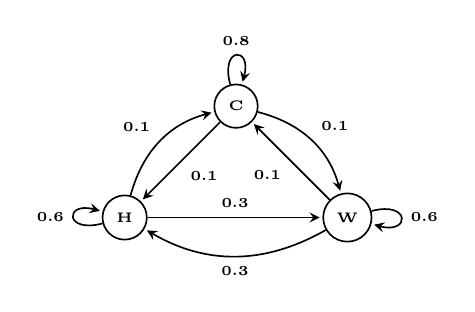
\begin{tikzpicture}[
			> = stealth, % arrow head style
			shorten > = 1pt, % don't touch arrow head to node
			auto,
			node distance = 2cm, % distance between nodes
			semithick, % line style
			font=\tiny\bfseries
			]
			
			\node[circle,draw] (qC) {C};
			\node[circle,draw] (qH) [below left of=qC] {H};
			\node[circle,draw] (qW) [below right of=qC] {W};
			
			\path[->] 	
			(qC) 	edge [loop above] node {0.8} ()
			edge [] node {0.1} (qH)
			edge [bend left] node {0.1} (qW)
			(qH) 	edge [loop left] node {0.6} ()
			edge [bend left] node {0.1} (qC)
			edge [] node {0.3} (qW)
			(qW)	edge [loop right] node {0.6} ()
			edge [bend left] node {0.3} (qH)
			edge [] node {0.1} (qC);
		\end{tikzpicture}
	\end{minipage}
	
	\begin{itemize}
		\item $\pi = [\pi_1, \pi_2, \ldots, \pi_n ]$: states initial probability distribution.
		\item $\sum_i \pi_i = 1$.
		\vspace{-6pt}\item E.g. \expword{Calculate $P(H\, W\, C\, C)$ where $\pi = [\overbrace{0.1}^C, \overbrace{0.7}^H, \overbrace{0.2}^W]$}.
	\end{itemize}
Hidden Markov model
	\begin{minipage}{.54\textwidth}
		\begin{itemize}
			\item $Q = \{q_1, q_2, \ldots, q_n\}$: states.
			\item $A$: transition probability matrix where $\sum_j a_{ij} = 1,\, \forall i$.
			\item $O = o_1 o_2 \ldots o_T$: sequence of observed events (words).
			\item $B = b_i(o_t)$: observation probabilities (\keyword{emission probabilities}), each represents the probability of generating an observation $o_t$ in a state $q_i$.
		\end{itemize}
	\end{minipage}
	\begin{minipage}{.45\textwidth}
		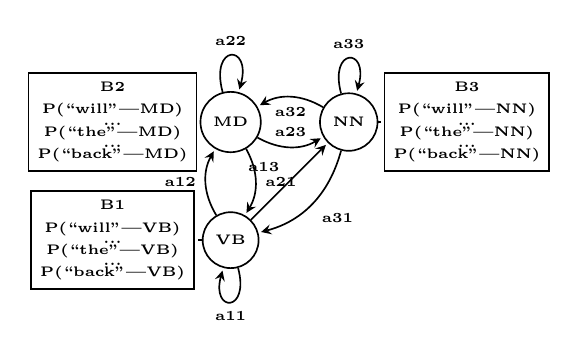
\begin{tikzpicture}[
			> = stealth, % arrow head style
			shorten > = 1pt, % don't touch arrow head to node
			auto,
			node distance = 1.5cm, % distance between nodes
			semithick, % line style
			font=\bfseries\fontsize{4}{4}\selectfont
			]
			
			\node[circle,draw] (q2) {MD};
			\node[align=center,draw] (q2e) [left of=q2] {B2\\ \\P(``will"|MD)\\...\\P(``the"|MD)\\...\\P(``back"|MD)};
			\node[circle,draw] (q3) [right of=q2] {NN};
			\node[align=center,draw] (q3e) [right of=q3] {B3\\ \\P(``will"|NN)\\...\\P(``the"|NN)\\...\\P(``back"|NN)};
			\node[circle,draw] (q1) [below of=q2] {VB};
			\node[align=center,draw] (q1e) [left of=q1] {B1\\ \\P(``will"|VB)\\...\\P(``the"|VB)\\...\\P(``back"|VB)};
			
			\path[->] 	
			(q1) 	edge [loop below] node {a11} ()
			edge [bend left] node {a12} (q2)
			edge [] node {a13} (q3)
			(q2) 	edge [loop above] node {a22} ()
			edge [bend left] node {a21} (q1)
			edge [bend right] node {a23} (q3)
			(q3)	edge [loop above] node {a33} ()
			edge [bend left] node {a31} (q1)
			edge [bend right] node {a32} (q2);
			
			\path[dashed] 	
			(q1) 	edge [] node {} (q1e)
			(q2) 	edge [] node {} (q2e)
			(q3) 	edge [] node {} (q3e);
			
		\end{tikzpicture}
	\end{minipage}
	
	\begin{itemize}
		\item $\pi = [\pi_1, \pi_2, \ldots, \pi_n ]$: states initial probability distribution.
		\item $\sum_i \pi_i = 1$.
	\end{itemize}
	
Training
	
	\begin{itemize}
		\item States are tags (categories) $t_i$.
		\item Let's define \keyword{START} as sentences' start tag.
		\item The observations $o_i$ are the words $w_i$.
		\item \keyword{C}: Number of occurrences in the training corpus.
	\end{itemize}
	
	\begin{block}{HMM training}
		\[
		\text{Transition probabilities: } P(t_i | t_{i-1}) = \frac{C(t_{i-1}, t_i)}{C(t_{i-1})} 
		\]\[
		\text{Emission probabilities: } P(w_i | t_i) = \frac{C(t_i, w_i)}{C(t_i)}
		\]\[
		\text{Initial distribution: } \pi_i = P(t_i | START) = \frac{C(START, t_i)}{C(START)}
		\]
	\end{block}

Labeling (tag decoding)
	
	\begin{itemize}
		\item Given
		\begin{itemize}
			\item a Markov model $\lambda = (A, B)$,
			\item an observations' sequence (words): $w = w_1 w_2 \ldots w_n$
		\end{itemize}
		\item Estimate a labels' sequence $\hat{t} = \hat{t}_1 \hat{t}_2 \ldots \hat{t}_n$
	\end{itemize}
	
	\begin{block}{Labels' decoding using HMM}
		\[
		\hat{t} = \arg\max\limits_t P(t | w) = \arg\max\limits_t \frac{P(w|t) P(t)}{P(w)} = \arg\max\limits_t P(w|t) P(t)%\text{ tel que } t = t_1 t_2 \ldots t_n
		\]
		
		\[ 
		P(w | t) \approx \prod\limits_{i=1}^n P(w_i|t_i) 
		\hskip2cm
		P(t) \approx \prod\limits_{i=1}^n P(t_i|t_{i-1}) 
		\]
		
		\[
		\hat{t} = \arg\max\limits_t \prod\limits_{i=1}^n P(w_i|t_i) P(t_i|t_{i-1})
		\]
	\end{block}

Viterbi algorithm
	
	\begin{block}{Viterbi}
		\scriptsize
		\begin{algorithm}[H]
			%				\vskip-1em
			\KwData{$w = w_1 \ldots w_T$, HMM $\lambda = (A, B)$ with $N$ states}
			\KwResult{$best\_path$, $prob\_path$}
			
			Create a matrix $viterbi[N, T]$\;
			
			\lForEach{state $ s = 1 \ldots N$}{
				$viterbi[s, 1] = \pi_s * b_s(w_1);\, backpointer[s, 1] = 0$
			}
			
			\ForEach{tag $ t = 2 \ldots T$}{
				\ForEach{state $ s = 1 \ldots N$}{
					$viterbi[s, t] = \max\limits_{s'=1}^N viterbi[s', t-1] * a_{s',s} * b_s(w_t)$\;
					$backpointer[s, t] = \arg\max\limits_{s'=1}^N viterbi[s', t-1] * a_{s',s} * b_s(w_t)$\;
				}
			}
			
			$prob\_path = \max\limits_{s=1}^N viterbi[s, T];\, pointer\_path = \arg\max\limits_{s=1}^N viterbi[s, T]$\;
			
			$best\_path$ is the path starting from $pointer\_path$ and following $backpointer$
			
			\Return $best\_path$, $prob\_path$\;
			
		\end{algorithm}
	\end{block}
	

\subsection{MEMM}

	
	\begin{itemize}
		\item Let $x_{n}^{m} = x_n x_{n+1} \ldots x_{m-1} x_m$
		\item Given 
		\begin{itemize}
			\item an observations sequence (words): $w = w_1 w_2 \ldots w_n$
			\item a set of features $f$ defined on the sequences (such as: majuscule word)
		\end{itemize}
		\item Estimate tags sequence $\hat{t} = \hat{t}_1 \hat{t}_2 \ldots \hat{t}_n$
	\end{itemize}
	
	\begin{block}{Labels decoding using MEMM}
		\[
		\hat{t} = \arg\max\limits_t P(t | w) = \arg\max\limits_t \prod\limits_{i}  P(t_i | w_i, t_{i-1})
		\]
		
		\[
		\hat{t} = \arg\max\limits_t \prod\limits_{i}  
		\frac{exp\left(\sum_j \theta_j f_j(t_i, w_{i-l}^{i+l}, t_{i-k}^{i-1})\right)}%
		{\sum_{t' \in tags} exp\left(\sum_j \theta_j f_j(t'_i, w_{i-l}^{i+l}, t_{i-k}^{i-1})\right)}
		\]
	\end{block}
	

\subsection{RNN}

Example
	
	\vgraphpage{seq_class_RNN_exp.pdf}
	

%===================================================================================
\section{Attention}
%===================================================================================

%	\begin{frame}
	%		\frametitle{ML for NLP}
	%		\framesubtitle{\insertsection}
	%		
	%		\begin{itemize}
		%			\item Attention mechanism is used to give more importance to some part of the input data more than others.
		%			\item It improves capturing long-term information.
		%		\end{itemize}
	%		
	%	\end{frame}

\subsection{Seq2Seq and attention}

Seq2Seq limits
	
	\begin{center}
		\hgraphpage[0.8\textwidth]{seq2seq_exp.pdf}
	\end{center}
	
	\begin{itemize}
		\item Model: Seq2Seq (Encoder-Decoder RNN)
		\item Long distant dependencies are forgotten.
		\item Next word generation depends only on the last words.
	\end{itemize}
	
Attention for seq2seq
	
	\begin{center}
		\hgraphpage[0.8\textwidth]{seq2seq_att_exp.pdf}
	\end{center}
	
	\vskip-6pt
	\begin{itemize}
		\item Keep the last encoded $T$ encoder's hidden states: $h_i$
		\item For each state $s_{t-1}$ of the decoder, its alignment with the hidden states is calculated.
		$ e_{t, i} = a(s_{t-1}, h_i) $
		\item Assign a weight to each hidden state: $\alpha_{t, i} = softmax(e_{t, i})$
		\item Calculate the state vector: $c_t = \sum_{i=1}^{T} \alpha_{t, i} h_i$
	\end{itemize}
	

\subsection{Attention}


	
	\begin{center}
		\hgraphpage[0.8\textwidth]{attention.pdf}
	\end{center}
	
	\vskip-6pt
	\begin{itemize}
		\item Keys ($k_i$): $m$ states which are used to estimate values' weights
		\item Values ($v_i$): $m$ states used to construct the context 
		\item Queries ($q_j$): current representation 
	\end{itemize}
	
	
	\begin{itemize}
		\item Let $ w_1 \cdots w_m $ a source sequence
		\begin{itemize}
			\item $ k_i =  Embedding_k(w_i)$ a vector of $ d $ elements
			\item $ v_i =  Embedding_v(w_i)$ a vector of $ v $ elements
		\end{itemize}
		\item Let $ w'_j $ a current target word
		\begin{itemize}
			\item $ q_j =  Embedding_q(w'_j)$ a vector of $ d $ elements
		\end{itemize}
		\item Calculate a similarity between each key $ k_i $ and our current target word 
		\[e_i = a(q_j, k_i)\]
		\item Calculate the percentage similarity (softmax can be masked)
		\[\alpha_i = softmax(e_i) = \frac{exp(e_i)}{\sum_k exp(e_k)}\] 
		\item The attention is a vector formed by cumulating percentages of each value vector
		\vspace{-6pt}\[attention(q, K, V) = \sum_{i=1}^{m} \alpha_i v_i\]
	\end{itemize}


Attention functions
	
	\[Q \in \mathbb{R}^{n \times d}, \, K \in \mathbb{R}^{m \times d}, \, a(Q, K) \in \mathbb{R}^{n \times m}, V \in \mathbb{R}^{m \times v} \]
	
	\begin{itemize}
		
		\item Dot product
		\[a(Q, K) = Q \cdot K^\top \]
		
		\item Scaled dot product 
		\[a(Q, K) = \frac{Q \cdot K^\top}{\sqrt{d}}\]
		
		\item Cosine similarity
		\[a(Q, K) = \frac{Q \cdot K^\top}{||Q|| \, ||K||}\]
		
		\item Additive attention (Bahdanau Attention)
		\[a(Q, K) = W_v^\top \cdot \tanh(W_q Q + W_k K)\]
	\end{itemize}
	
Self-attention
	
	\begin{itemize}
		\item \textbf{GOAL}: Encoding a sequence element based on the elements of the same sequence.
		\item \textbf{Eg.}: \expword{Encoding a word in a sentence to capture its semantic representation}.
		\item \textbf{Method}:
		\begin{itemize}
			\item Use MLPs to represent words as queries, keys and values.
			\item Set a maximum number of elements in a sequence.
			\item Truncate sequences that exceed this number.
			\item Complete those that do not reach this number with a predefined code.
			\item For each word, the output of attention is its encoding according to its context (words of the same sentence)
		\end{itemize}
	\end{itemize}
	
Self-attention (Example)
	
	\begin{center}
		\vgraphpage{self-attention_exp.pdf}
	\end{center}
	


\subsection{Transformers}

Multi-Head Attention
	
	\vspace{-6pt}
	\begin{figure}
		\centering
		\hgraphpage[0.9\textwidth]{multi_head_att_.pdf}
		\vspace{-6pt}
		\caption{Multi-Head Attention \cite{2017-vaswani-al}}
	\end{figure}
	
Multi-Head Attention (Annoying formulas)
	
	\[Q \in \mathbb{R}^{n \times d}, \, K \in \mathbb{R}^{m \times d}, \, MultiHead \in \mathbb{R}^{n \times d_{model}}, V \in \mathbb{R}^{m \times v} \]
	
	\[W^Q_i \in \mathbb{R}^{d_{model} \times d}, \,  W^K_i \in \mathbb{R}^{d_{model} \times d}, \, W^V_i \in \mathbb{R}^{d_{model} \times v}, \, W^O \in \mathbb{R}^{hv \times d_{model}}\]
	
	\[head_i = Attention(Q W^Q_i, K W^Q_i, V W^V_i)\]
	
	\[MultiHead(Q, K, V) = Concat(head_1, \ldots, head_h) \cdot W^O\]
	


Architecture
	
	\begin{minipage}{0.49\textwidth}
		\begin{figure}
			\centering
			\hgraphpage[0.68\textwidth]{transformers_.pdf}
			\vskip-8pt
			\caption{Transformers' architecture \cite{2017-vaswani-al}}
		\end{figure}
	\end{minipage}
	\begin{minipage}{0.1\textwidth}
		=
	\end{minipage}
	\begin{minipage}{0.39\textwidth}
		\hgraphpage[\textwidth]{transformers.pdf}
	\end{minipage}

Encoder
	\begin{itemize}
		\item Encodes each input element based on its context (the entire input).
		\item Uses multi-head self-attention
		\item Completely bi-directional
		\begin{itemize}
			\item In BiRNN architecture, the encoder represents long-term relation indirectly (using a context).
			\item In Encoders it is directly represented, but the notion of element's position is lost.
		\end{itemize} 
		\item We can introduce position's embedding into the word's initial representation (before being transformed into keys, values and queries).
	\end{itemize}

Decoder
	\begin{itemize}
		\item \keyword{Autoregressive}: The output is a \optword{direct} function of the past elements
		\[\hat{y}_t = \sum_{i = 1}^{\rho} \varphi_{i} y_{t-i} + \epsilon_t\]
		\item Not as RNNs where the dependence is indirect
		\[\hat{y}_t = \arg\max_y p(y | X;\ y_1, \cdots, y_{i-1};\ W;\ b)\]
		\item Each time an element is generated, it will be added into the input to generate the next element.
		\item To stop generating, a maximum size is used. Also, a special token is used to mark the end of generation.
	\end{itemize}

Pretrained models (BERT: Enc) \cite{devlin-etal-2019-bert}
	\begin{center}
		%			\hgraphpage[0.95\textwidth]{bert-arch.pdf}
		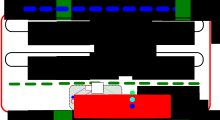
\includegraphics[width=0.95\textwidth]{../img/word-sem/bert-arch.pdf}
	\end{center}

Pretrained models (GPT: Dec) \cite{radford2018improving}
	\begin{figure}[htbp]
		\hgraphpage[\textwidth]{gpt-arch_.pdf}
		\caption{GPT's architecture and different tasks \cite{radford2018improving}}
	\end{figure}

Pretrained models (T5: Enc-Dec) \cite{T5}
	\begin{figure}[htbp]
		\hgraphpage[\textwidth]{t5-arch_.pdf}
		\caption{T5's (Text-to-Text Transfer Transformer) training \cite{T5}}
	\end{figure}

Pretrained models (BART: Enc-Dec) \cite{bart}
	\begin{figure}[htbp]
		\centering
		\hgraphpage[0.58\textwidth]{bart-arch1_.pdf}
		\hgraphpage[0.4\textwidth]{bart-arch2_.pdf}
		\caption{BART's training \cite{bart}}
	\end{figure}




\begin{discussion}
	
	Can you understand this sentence? Regardless of your answer (yes or no), you certainly understood the question; otherwise, you wouldn't have answered in the first place. Imagine a machine that can reason like that. Imagine that it can understand your language and respond in a similar way to yours. This was considered science fiction in the '50s. It still is, but nowadays we are closer to this dream than before. The field of NLP, and AI in general, has gone through beautiful periods and other challenging ones. Throughout its evolution, even in the midst of winter, there were always scholars who fought to advance this field and to reach this dream. The fight continues...
	
	
\end{discussion}


%=====================================================================
\ifx\wholebook\relax\else
% \cleardoublepage
% \bibliographystyle{../use/ESIbib}
% \bibliography{../bib/RATstat}
	\end{document}
\fi
%=====================================================================


% !TEX TS-program = xelatex
% !TeX program = xelatex
% !TEX encoding = UTF-8
% !TEX spellcheck = en_US

%=====================================================================
\ifx\wholebook\relax\else
	\documentclass{KBook}
	\input{calls}
	\begin{document}
		\mainmatter
	
\fi
%=====================================================================
\changegraphpath{../img/basic/}

\chapter{Basic Text Processing}

\begin{introduction}[NA\textcolor{white}{T}. LANG. PROC.]
	%	\lettrine{A}{fin} de traiter un langage, nous commençons par sa plus petite unité : le graphème. 
	\lettrine{T}{o} process a language, we start with its smallest unit: the grapheme. 
	In computer science, graphemes along with punctuation and spacing are called characters. 
	There are operations that allow us to search for and compare strings of characters.
	By combining characters, we get a text with sentences and words. 
	Given a text, we should be able to segment it into sentences and a sentence into words. 
	The latter can be unnecessary for certain tasks, such as prepositions in information retrieval. 
	Thus, they need to be filtered before applying this task. 
	Also, words can have multiple morphological variations. 
	If we want to process a single variation, we need to normalize them. 
	In addition, we should be able to generate these variations or switch from one variation to another given a word form. 
	This chapter summarizes some tasks at the morphological level of languages (lexical analysis).
\end{introduction} 

According to Larousse, a character in computing and telecommunications is defined as: ``\textit{Any symbol (digit, letter of the alphabet, punctuation mark, etc.) used to represent data for processing or transmission purposes.}".
A word is composed of several characters according to a regular language. 
A sentence, in turn, consists of several words according to a context-free language (in most languages). 
This last proposition concerns the syntactic level.
For now, we are interested in the morphological level or what is called lexical analysis.
The points addressed in this chapter are as follows: 
\begin{itemize}
	\item Searching in the text using regular expressions. 
	Among the applications: data extraction (dates, phone numbers, email addresses, etc.).
	
	\item Comparing strings of characters using edit distance. 
	Among its applications: spell correction and approximate search.
	
	\item Text segmentation into sentences and sentences into words. 
	
	\item Text normalization to reduce word variations.
	
	\item Word formation in synthetic languages and the reverse operation.
\end{itemize}

\section{Character Processing}

Here, we consider a text as a sequence of characters. 
In a more formal way, a text can be composed using a finite state automaton where the vocabulary is the set of characters. 
To search for substrings of characters in a text, we can use regular expressions recognizing type 3 languages (regular languages) in the Chomsky hierarchy. 
Searching for sequences in a text allows us to replace or separate them (e.g., \expword{word separation}). 
Another type of search is approximate search: looking for parts almost similar to a given string. 
To do this, we must be able to compare two strings of characters by measuring the difference between them. 
One of the techniques used is edit distance.

\subsection{Regular Expressions}

A regular expression, called \keyword[R]{RegEx}, is a sequence of characters specifying a search pattern.
Several programming languages provide the ability to search and replace using regular expressions. 
To use it for search, a regular expression is transformed into a finite state automaton (FSA) which is then transformed into a deterministic FSA.
A dot in a regular expression represents any character.
If we want to search for a dot and not any character, we need to add a backslash before the dot.
We can design a complex regular expression by composing several simple regular expressions.
These are described in Table \ref{fig:exp-reg} with their meanings and examples.

\begin{table}[ht]
	\begin{tabular}{p{.1\textwidth}p{.34\textwidth}p{.46\textwidth}}
		\hline\hline
		\textbf{RE} & \textbf{Meaning} & \textbf{Example} \\
		\hline
		
		. & any character & /beg.n/ : \expword{I \underline{begun} at the \underline{begin}ning} \\
		
		\empty [aeuio] & specific characters & /[Ll][ae]/ : \expword{\underline{Le} chat mange \underline{la} sourie} \\
		
		\empty [a-e] & range of characters & /[A-Z]../ : \expword{\underline{J'a}i vu \underline{Kar}im} \\
		
		\empty [\textasciicircum aeuio] & exclude characters & /[\textasciicircum A-Z]a./ : \expword{J\underline{'ai} vu Karim} \\
		
		c? & zero or one & /colou?r/ : \expword{It is \underline{colour} or \underline{color}} \\
		
		c* & zero or more & /No*n/ : \expword{\underline{Nn}! \underline{Non}! \underline{Nooooooon}!} \\
		
		c+ & one or more & /No+n/ : \expword{Nn! \underline{Non}! \underline{Nooooooon}!} \\
		
		c\{n\} & n occurrences & /No\{3\}n/ : \expword{Nn! Non! Noon! \underline{Nooon}!} \\
		
		c\{n,m\} & n to m occurrences & /No\{1,2\}n/ : \expword{Nn! \underline{Non}! \underline{Noon}! Nooon!} \\
		
		c\{n,\} & at least n occurrences & /No\{2,\}n/ : \expword{Nn! Non! \underline{Noon}! \underline{Nooon}!} \\
		
		c\{,m\} & at most m occurrences & /No\{,2\}n/ : \expword{\underline{Nn}! \underline{Non}! \underline{Noon}! Nooon!} \\
		
		\hline 
		
		\textbackslash d & [0-9] & /\textbackslash d\{2,\}/ : \expword{The year \underline{1962}}\\
		
		\textbackslash D & [\textasciicircum 0-9] & /\textbackslash D\{2,\}/ : \expword{\underline{The year }1962}\\
		
		\textbackslash w & [a-zA-Z0-9\_] & /\textbackslash w\{2,\}/ : \expword{\underline{The} \underline{year} 1962}\\
		
		\textbackslash W & [\textasciicircum \textbackslash w] & /\textbackslash W\{2,\}/ : \expword{\underline{The year} \underline{1962}}\\
		
		\textbackslash s & [ \textbackslash r\textbackslash t\textbackslash n\textbackslash f] & /\textbackslash s+/ : \expword{\underline{The year}\underline{ }1962\underline{ }}\\
		
		\textbackslash S & [\textasciicircum \textbackslash s] & /\textbackslash S+/ : \expword{\underline{The year} \underline{1962}}\\
		
		\hline 
		
		( ) & grouping & /(bla)+/ : \expword{This is \underline{blabla}}\\
		
		\textbar & disjunction & /continu(er\textbar ation)/ : \expword{I \underline{continue} the \underline{continuation}} \\
		
		\textasciicircum  & start of text & /\textasciicircum K/ :  \expword{\underline{K}ill Karim}\\
		
		\$ & end of text & /\textbackslash .[\textasciicircum .]+\$/ :  \expword{file.tar\underline{.gz}}\\
		
		\hline\hline
	\end{tabular}
	
	\caption{Regular expressions.}
	\label{fig:exp-reg}
\end{table}

The most common use of regular expressions is searching for substrings of characters in a large text.
Most text editors and programming languages provide mechanisms to use regular expressions.
Using patterns to search for strings makes regular expressions a very powerful tool for data extraction.
For example, we can use regular expressions to extract emails from blogs and social networks.
Let's take an example of a regular expression \expword{/[a-zA-Z]\textbackslash w*(@| at )[a-zA-Z]\textbackslash w+\textbackslash .[a-zA-Z]\{2,3\}/} to search for email addresses.
The part \expword{/[a-zA-Z]/} ensures that both the username and the domain name start with a letter.
The username accepts at least one character since the first letter is followed by \expword{/\textbackslash w*/}, meaning zero or more characters of type letter, digit, or underscore.
The domain name in this regular expression accepts at least two characters since the first letter is followed by \expword{/\textbackslash w+/}, meaning one or more characters of type letter, digit, or underscore.
The username and domain name are separated either by an ``\expword{@}" or by ``\expword{ at }"; this is indicated by \expword{/(@| at )/}.
The domain extension must always be preceded by a dot; here, we use \expword{/\textbackslash ./} to indicate that it is the dot character.
Otherwise, if we used \expword{/./}, it represented any character.
The extension is composed of two to three letters.
Here are some emails that we can extract using this regular expression: 
``\expword{ab\_aries@esi.dz}", ``\expword{ab\_ARIES@eSi.dz}", ``\expword{ab\_aries at esi.dz}", ``\expword{a@es.edu}", ``\expword{a1@e2s.edu}".

To capture a string, we use grouping with the group number.
Group number "N" must be preceded by a special character, often ``\$" or ``\textbackslash".
An example of text replacement in a text editor (``kate" in our case) is illustrated in Figure \ref{fig:kate_regex}.
Here, we search for the word ``cat" to replace it with the word ``dog". 
But, we want to keep ``ch" as it is shared between the two words.
In this case, we capture the string ``ch" to keep it and replace the rest: ``at" with ``ien".


Perhaps the utility of grouping is not clear with the previous example since we have only one string to capture.
If we had a disjunction, it would be more interesting.
Let's take the example: ``\expword{I like cats because they are more useful than rats.}".
If we replace the string ``at" in both ``cat" and ``rat" with ``ock", we would have the following text:
``\expword{I like clocks because they are more useful than rocks.}".
In this case, we need to test the words ``chat" and ``rat" to replace only the last part and keep the first part intact.
Several programming languages provide string replacement using \keyword[R]{RegEx}.
In Javascript, strings are assigned a ``replace" method to replace one of their parts with another string.
If we want to replace all occurrences, we should use the ``g" flag after the regular expression.
To retrieve the captured group, we use ``\$" followed by the group's order.

\begin{lstlisting}[language={[KB]Javascript}, style=codeStyle]
	let orig = "I like cats because they are more useful than rats.";
	let remp = orig.replace(/[cr]at/g, "$1ock");
\end{lstlisting}

For any use of regular expressions in Python, we need to use the ``re" module.
A regular expression is a string preceded by the ``r" indicator.
To retrieve the captured group, we use ``\textbackslash".

\begin{lstlisting}[language=Python, style=codeStyle]
	import re
	orig = "I like cats because they are more useful than rats."
	remp = re.sub(r'[cr]at', r'\1ock', orig)
\end{lstlisting}


\subsection{Edit Distance}

Sometimes, when we write using our computers, we make typos; we can insert an extra character, duplicate a character, etc. 
Such an operation is called an "edit operation". 
We can compare two strings by counting the number of edit operations to change from an original string to a modified one. 
The different edit operations are as follows (where $X$ is the set of characters in the language):
%
\begin{itemize}
	\item \optword{Insertion}: inserting a character into a string ($uv \rightarrow uxv \,/\, u, v \in X^*;\, uv \in X^+;\, x \in X$). 
	
	For example, \expword{courir $ \rightarrow $ courrir, entraînement $ \rightarrow $ entraînnement}.
	
	\item \optword{Deletion}: deleting a character from a string ($uxv \rightarrow uv \,/\, u, v \in X^*;\, uv \in X^+;\, x \in X$). 
	
	For example, \expword{héros $ \rightarrow $ héro, meilleur $ \rightarrow $ meileur}.
	
	\item \optword{Substitution}: substituting one character for another ($uxv \rightarrow uyv \,/\, u, v \in X^*;\, x, y \in X;\, x \ne y$). 
	
	For example, \expword{cela $ \rightarrow $ celà, croient $ \rightarrow $ croyent }
	
	\item \optword{Transposition}: changing the order of two characters ($uxwyv \rightarrow uywxv \,/\, u, v, w \in X^*;\, x, y \in X;\, x \ne y$). 
	
	For example, \expword{cueillir $ \rightarrow $ ceuillir}.
\end{itemize}

Knowing the number of edit operations allows us to compare two strings. There are several examples of using edit distance (number of modifications):
\begin{itemize}
	\item \optword{File revision}: for example, the Unix command "\expword{diff}" that compares two files.
	\item \optword{Spelling correction}: suggesting possible corrections for a mistake (e.g., \expword{Hunspell}).
	\item \optword{Plagiarism detection}: here, we use words instead of characters.
	\item \optword{Spam filtering}: sometimes, spammers intentionally make spelling mistakes to deceive the spam detection tool.
	\item \optword{Bioinformatics}: quantifying the similarity between two DNA sequences.
\end{itemize}

\subsubsection{Hamming Distance}

This distance allows only substitution. The strings must be of the same length. Among its uses, we can mention the detection of data transmission errors.\newline
For example, \expword{D(010\underline{0}101\underline{0}01\underline{1}0, 010\underline{1}101\underline{1}01\underline{0}0) = 3}.
To calculate the distance, we compare the two strings character by character to get the number of different characters (see Algorithm \ref{algo:hamming}).

\begin{algorithm}[ht]
	\KwData{orig, modif}
	\KwResult{distance: integer}
	distance $\leftarrow$ 0\;
	
	\For{pos $ \in 1 \ldots |orig|$}{
		\If{orig[pos] $\ne$ modif[pos]}{
			distance $\leftarrow$ distance + 1
		}
	}
	
	\caption{Calculation of Hamming Distance \label{algo:hamming}}
	
\end{algorithm}



\subsubsection{Longest Common Subsequence}

This distance allows insertion and deletion. Among its uses is the detection of changes in the "diff" program (also used in "Git"). In English, it is called "Longest Common Subsequence" (LCS). Given two strings $X$ and $Y$ with lengths $n$ and $m$ respectively, we define a two-dimensional array $C[m, n]$ containing the length of the LCS. Equation \ref{eq:LCS-length} can be used to calculate the length of the longest subsequence.
\begin{equation}
	C[i, j] =  
	\begin{cases}
		0 & \text{If } i = 0 \text{ or } j=0\\
		C[i-1, j-1] + 1 & \text{If } i,j > 0 \text{ and } x_i = y_j\\
		\max (C[i, j-1], C[i-1, j]) & \text{If } i,j > 0 \text{ and } x_i \ne y_j\\
	\end{cases}
	\label{eq:LCS-length}
\end{equation}

In this case, the length of the longest subsequence $|LCS(X, Y)| = C[m, n]$. The distance will be calculated using Equation \ref{eq:LCS-distance}.
\begin{equation}
	D(X, Y) = m + n - 2 |LCS(X, Y)|
	\label{eq:LCS-distance}
\end{equation}

\subsubsection{Levenshtein Distance}

This distance allows insertion, deletion, and substitution. In general, it is used in approximate search and spell checking. Given two strings $X$ and $Y$ with lengths $n$ and $m$ respectively, we define an array $D[m, n]$ with two dimensions containing the edit distance between the substrings $X[1..i]$ and $Y[1..j]$. In this case $D[0, 0] = 0$, and the final distance will be stored in $D[m, n]$. Equation \ref{eq:lev-distance} formulates how to calculate this distance (using dynamic programming). It should be noted that in this version, the cost of deletion and insertion is $1$, and the cost of substitution is $2$.
\begin{equation}
	D[i, j] = \min 
	\begin{cases}
		D[i - 1, j] + 1 \text{ //Deletion}\\
		D[i, j-1] + 1 \text{ //Insertion}\\
		D[i-1, j-1] + \begin{cases}
			2 & \text{if } x_i \ne y_j \\
			0 & \text{otherwise}
		\end{cases}
	\end{cases}
	\label{eq:lev-distance}
\end{equation}

For example, \expword{D(amibe, immature) = 9}. In this case, "a" and "m" are deleted (1+1); "i" remains the same (0); the characters "m", "m", "a", "t", and "u" are inserted (1+1+1+1+1), "b" is substituted by "r" (2), and "e" remains the same (0). The calculation is illustrated in Figure \ref{fig:laven-distance}, where the arrows represent where the value comes from, and the colored cells represent the chosen path. Of course, we can choose another path that gives another interpretation. To help choose the path, we can use probabilities of edit operations. For example, in spell correction, letters are more likely to be replaced by others (those adjacent on the keyboard).


\subsubsection{Damerau–Levenshtein Distance}

This distance allows insertion, deletion, substitution, and transposition between two adjacent characters. Generally, it is used in spell checking. This distance is calculated like Levenshtein, adding transposition between two adjacent characters. Equation \ref{eq:lev-dem-distance} represents how to calculate this distance. In this version, we have tried to assign a weight of $1$ for all edit operations.
\begin{equation}
	D[i, j] = \min 
	\begin{cases}
		D[i - 1, j] + 1 \text{ //Deletion}\\
		D[i, j-1] + 1 \text{ //Insertion}\\
		D[i-1, j-1] + \begin{cases}
			1 & \text{if } x_i \ne y_j \text{ //Substitution}\\
			0 & \text{otherwise}
		\end{cases}\\
		D[i-2, j-2] + 1 \text{ if } x_i = y_{j-1} \text{ and } x_{i-1} = y_j \text{ //Transposition}\\
	\end{cases}
	\label{eq:lev-dem-distance}
\end{equation}

For example, \expword{D(amibe, immature) = 6}. In this case, "i" and "m" are inserted (1+1); "a" is transposed with "m" (1); "t" is inserted (1); "i" is substituted by "u" (1); "b" is substituted by "r" (1), and "e" remains the same (0). The calculation is illustrated in Figure \ref{fig:dam-laven-distance}, where the arrows represent where the value comes from, and the colored cells represent the chosen path. When there is a transposition, we skip two diagonal cells.
\begin{figure}[ht]
	\centering
	\begin{tabular}{|r|r|r|r|r|r|r|r|r|r|}
		\hline
		&\bfseries \# &\bfseries i &\bfseries m &\bfseries m &\bfseries a &\bfseries t &\bfseries u &\bfseries r &\bfseries e \\
		\hline
		\bfseries \# & 0 & \cellcolor{green!25} $ \leftarrow $ 1 & \cellcolor{green!25} $ \leftarrow $ 2 & $ \leftarrow $ 3 & $ \leftarrow $ 4 & $ \leftarrow $ 5 & $ \leftarrow $ 6 & $ \leftarrow $ 7 & $ \leftarrow $ 8\\
		\hline
		\bfseries a & $ \uparrow $ 1 & $ \nwarrow $ 1 & $ \nwarrow\leftarrow $ 2 & $ \nwarrow\leftarrow $ 3 & $ \nwarrow $ 3 & $ \leftarrow $ 4 & $ \leftarrow $ 5 & $ \leftarrow $ 6 & $ \leftarrow $ 7 \\
		\hline
		\bfseries m & $ \uparrow $ 2 & $ \nwarrow\uparrow $ 2 & $\nwarrow $ 1 & $\nwarrow\leftarrow $ 2 & \cellcolor{green!25} $\leftrightharpoons\leftarrow $ 3 & \cellcolor{green!25} $\leftarrow $ 4 & $\leftarrow $ 5 & $\leftarrow $ 6 & $\leftarrow $ 7\\
		\hline
		\bfseries i & $ \uparrow $ 3 & $ \nwarrow $ 2 & $\leftrightharpoons\uparrow $ 2 & $\nwarrow\leftarrow\uparrow $ 3 & $\nwarrow $ 3 &  $\nwarrow\leftarrow $ 4 & \cellcolor{green!25} $\nwarrow\leftarrow $ 5 & $\nwarrow\leftarrow $ 6 & $\nwarrow\leftarrow $ 7\\
		\hline
		\bfseries b & $ \uparrow $ 4 & $ \uparrow $ 3 & $\nwarrow\uparrow $ 3 & $\nwarrow $ 3 & $\nwarrow\leftarrow\uparrow $ 4 & $\nwarrow $ 4 & $\nwarrow\leftarrow $ 5 & \cellcolor{green!25} $\nwarrow\leftarrow $ 6 & $\nwarrow\leftarrow $ 7\\
		\hline
		\bfseries e & $ \uparrow $ 5 & $ \uparrow $ 4 & $\nwarrow\uparrow $ 4 & $\nwarrow\uparrow $ 5 & $\nwarrow $ 4 & $\nwarrow\leftarrow\uparrow $ 5 & $\nwarrow $ 5 & $\nwarrow\leftarrow $ 6 & \cellcolor{green!25} $\nwarrow $ 6\\
		\hline
	\end{tabular}
	\caption[Example of Damerau–Levenshtein Distance calculation.]{Example of Damerau–Levenshtein Distance calculation between the words "amibe" and "immature".}
	\label{fig:dam-laven-distance}
\end{figure}

\subsubsection{Jaro Distance}

This distance allows only transposition. In reality, it is a similarity measure that returns a value between $0$ (no similarity) and $1$ (similar). It is used for calculating similarity between named entities, etc. Given two strings $X$ and $Y$ with lengths $n$ and $m$ respectively, we calculate the number of matching characters $c$ and the number of transpositions $t$. The Jaro distance is calculated according to Equation \ref{eq:jaro-distance}.
\begin{equation}
	D(X, Y) = 
	\begin{cases}
		0 & \text{if } c = 0\\
		\frac{1}{3} (\frac{c}{m} + \frac{c}{n} + \frac{c-t}{c}) & \text{otherwise}
	\end{cases}
	\label{eq:jaro-distance}
\end{equation}

The number of matching characters $c$ is the number of identical characters in $X$ and $Y$ with a separation $ e= \max (m, n)/2 - 1$. In this case, if we are at character $i$ (going from $0$ to $n-1$) of word $X$, we start the comparison from character $j=\max(0, i - e)$ of word $Y$ and end at character $j=\min(i+e, m-1)$.
In this operation, we can prepare two boolean vectors indicating the position of the character having a match in the other word.
%
The number of transpositions $t$ is calculated by comparing the i\textsuperscript{th} matching character of $X$ with the i\textsuperscript{th} matching character of $Y$. We count the number of times $x_i \ne y_i$ and divide it by two (see Algorithm \ref{algo:jaro-transpo}).
\vspace{-6pt}
\begin{algorithm}[ht]
	\KwData{Xmatch, Ymatch : boolean vectors}
	\KwResult{t: integer}
	t $\leftarrow$ 0 ; j $\leftarrow$ 0\;
	
	\Pour{i $ \in 0 \ldots m$ }{
		\Si{Xmatch[i] = True}{
			\lTq{Ymatch[j] $\ne$ True}{
				j $\leftarrow$ j + 1
			}
			
			\lSi{$x_i \ne y_j$}{
				t $\leftarrow$ t + 1
			}
			j $\leftarrow$ j + 1\;
		}
	}
	
	t $\leftarrow$ t/2\;
	
	\caption{Calculation of the number of transpositions between two words X and Y in Jaro Distance \label{algo:jaro-transpo}}
	
\end{algorithm}

Let's take the example of "amibe" and "immature" with lengths 5 and 8 respectively. The separation will be $e=\max(5, 8)/2 - 1 = 3$. Figure \ref{fig:jaro} represents the calculation of the distance between these two words using the two possible orders. In the matrix, $0$ means "False" and $1$ means "True" (match). The bold cells represent the search range using the separation of 3. The underlined cells represent the intersection between the i\textsuperscript{th} match of X and the i\textsuperscript{th} match of Y. The underlined matches of the vectors of the two words represent transpositions.

%===================================================================================
\section{Text Segmentation}
%===================================================================================

Text can be processed when segmented into smaller passages; these can be chapters, paragraphs, sentences, or words depending on the desired granularity. In several languages, sentences are delimited by a period or a specific mark, and words are delimited by spaces. Even in these languages, the delimiter can be used for other purposes. There are languages where there is no sentence or word delimiter or both.

\subsection{Sentence Delimitation}

To separate sentences in a semi-structured format, such as HTML, we can use markers like the \expword{\textless P\textgreater} tag. However, when dealing with unstructured text, many languages use markers like the period, exclamation point, and question mark to mark the end of a sentence. In this case, we can use a simple regular expression \expword{/[.?!]/} to delimit sentences in languages like French, English, etc. Sometimes we want to separate long sentences with clauses separated by commas. Also, quotes can cause a problem: is the sentence inside separated, or is it a continuation of the main clause? For example, \expword{He said, "I'm tired." returning to his bed.} The period in these languages is not always used to separate sentences. It can be used in numbers: \expword{123,456.78 (American style) 123.456,78 (European style)}. Abbreviations like "Mr.," "Dr.," and "etc." contain periods and can be in the middle of a sentence. They can also be at the end; so, you really need to be able to detect abbreviations and whether they mark the end of the sentence or not. If all of this doesn't seem problematic, we can always try to separate sentences in Thai. This language does not use markers to separate sentences.

When the sentence marker is reserved for other uses, there are always factors that help the reader decide whether it is a sentence delimiter or not. These factors can be extracted by observing how the language defines the end of a sentence. Some contextual factors have been proposed and used for sentence segmentation \cite{10-palmer}:
\begin{itemize}
	\item \optword{Case}: Sentences always start with an uppercase letter. But, this is not always the case; we can find an abbreviation followed by a proper name (e.g., "Mr. Aries"). In addition, it is not guaranteed that the writer respects writing rules. We can see this, for example, on social networks where many rules are abandoned.
	
	\item \optword{Proper Names}: Proper names start with an uppercase letter; they may not be the beginning. In the previous example ("Mr. Aries"), we can deduce that the period does not represent a separation since both words start with an uppercase letter, and the second is a proper name. In this case, the probability that the first is an abbreviation is high, especially if the word is in the middle of the sentence.
	
	\item \optword{Grammatical Category}: The categories of words surrounding the period can help the decision (boundary or not). In fact, \citet{97-palmer-hearst} were able to improve sentence boundary detection by using the grammatical categories of the two words before and after the period with a machine learning algorithm.
	
	\item \optword{Word Length}: Abbreviations are shorter.
	
	\item \optword{Prefixes and Suffixes}: Words with affixes are less likely to be abbreviations.
	
	\item \optword{Abbreviation Classes}: Abbreviations can be at the end of the sentence. But, there is a set of abbreviations that are always followed by another word, such as "Mr." \citet{89-riley,97-reynar-ratnaparkhi} divide abbreviations into two categories: titles (which cannot be at the end of a sentence (e.g., "Mr.", "Dr.", etc.) and corporate indicators (which can be at the end of a sentence (e.g., "Corp.", "S.P.A.", etc.)).
\end{itemize}

Automatic detection of sentence boundaries can be accomplished using manual rules or using machine learning. In the first approach, we can use regular expressions to detect delimiters. Then, we can use a list of abbreviations to improve the decision. Rules can be enriched by introducing the factors discussed earlier. To avoid manually writing these rules, we can use a machine learning algorithm that classifies the period as a delimiter/non-delimiter based on these same rules.


\subsection{Word Segmentation}

Several languages (Arabic, French, English, etc.) use space as a word delimiter. 
A simple regular expression like \expword{/[ ]+/} can be used to separate words. 
But sometimes we want to retrieve an expression with multiple words; like the case of dates, numbers, etc. 
An example of numbers is "\expword{nine hundred forty five}"; this expression can be considered a single token in some processing. 
In some languages, the apostrophe can be a source of ambiguity. In English, the apostrophe can be used with an "\textit{s}" in the possessive form (\expword{Karim's thesis}), contractions (\expword{she's, it's, I'm, we've}), or in the plural of some words (\expword{I.D.'s, 1980's}). In French, there are quite a few examples of contractions: contraction of articles (\expword{l'homme, c'était}), contraction of pronouns (\expword{j'ai, je l'ai}), and other forms (\expword{n'y, qu'ils, d'ailleurs}). Some languages use compound words, either by composition or by hyphen. In German, it is common to use word composition: noun-noun (\expword{Lebensversicherung: life insurance}), adverb-noun (\expword{Nichtraucher: non-smoker}), and preposition-noun (\expword{Nachkriegszeit: post-war period}). Other languages use the hyphen, such as English (\expword{end-of-file, classification-based}) and French (\expword{va-t-il, c'est-à-dire, celui-ci}). There are languages, like Japanese, that do not use markers to separate words (\expword{今年は本当に忙しかったです。}).

There are two approaches to word segmentation: rule-based and statistical. The rule-based approach mainly uses regular expressions based on morphological rules. It can also use word lists. For example, in a \keyword{Scriptio Continua}-type language like Japanese and Chinese, we can use a dictionary and compare words by starting from the end by taking the longest sequence. The statistical approach uses a language model to calculate the probability that a character marks the end of a word. Language models will be presented in the next chapter.


%Approches
%\begin{itemize}
%	\item Par règles : en utilisant des expressions régulières 
%	\begin{itemize}
%		\item \url{https://www.nltk.org/api/nltk.tokenize.html}
%		\item \url{https://nlp.stanford.edu/software/tokenizer.shtml}
%		\item \url{https://spacy.io/}
%		\item \url{https://github.com/kariminf/jslingua}
%		\item \url{https://github.com/linuxscout/pyarabic}
%	\end{itemize}
%	\item Statistique : en utilisant un modèle de langue pour calculer la probabilité qu'un caractère marque la  fin d'un mot 
%	\begin{itemize}
%		\item \url{https://nlp.stanford.edu/software/segmenter.html}
%		\item \url{https://opennlp.apache.org/}
%	\end{itemize}
%\end{itemize}

%===================================================================================
\section{Text Segmentation}
%===================================================================================

A text can be processed when it is segmented into smaller units; these can be chapters, paragraphs, sentences, or words depending on the desired granularity. 
In several languages, sentences are delimited by a period or a specific mark, and words are delimited by spaces. 
Even in these languages, the delimiter may be used for other purposes. 
There are languages where there is no sentence or word delimiter, or both.

\subsection{Sentence Delimitation}

To separate sentences in a semi-structured format, such as HTML, we can use markers like the \expword{\textless P\textgreater} tag. 
However, when it comes to unstructured text, many languages use markers like the period, exclamation mark, and question mark to mark the end of a sentence. 
In this case, we can use a simple regular expression \expword{/[.?!]/} to delimit sentences in languages like French, English, etc. 
Sometimes, we want to separate long sentences with clauses separated by commas. 
Also, quotes can cause a problem: is the sentence inside separated, or is it a continuation of the main clause? 
For example, \expword{He said, "I am tired," returning to his bed.}.
The period in these languages is not always used to separate sentences. 
It can be used in numbers: \expword{123,456.78 (American style) 123.456,78 (European style)}.
Abbreviations like "Mr.", "Dr.", and "etc." contain periods and may appear in the middle of a sentence. 
They can also appear at the end; so, we really need to be able to detect abbreviations and whether they mark the end of a sentence or not. 
If all this doesn't seem problematic, we can still try separating Thai sentences. 
This language does not use markers to separate sentences.

When the sentence marker is reserved for other uses, there are always factors that help the reader decide whether it is a sentence delimiter or not. 
These factors can be extracted by observing how the language defines the end of the sentence. 
Some contextual factors have been proposed and used for sentence segmentation \cite{10-palmer}:
\begin{itemize}
	\item \optword{Casing}: Sentences always begin with an uppercase letter. 
	But, this is not always the case; we can find an abbreviation followed by a proper noun (Ex. "\expword{Mr. Aries}"). 
	Moreover, it is not guaranteed that the writer follows the writing rules. 
	We can see this, for example, in social networks where several rules are abandoned.
	
	\item \optword{Proper Names}: Proper names start with an uppercase letter; they may not be the beginning. 
	In the previous example ("\expword{Mr. Aries}"), we can deduce that the period does not represent a separation since both words start with an uppercase letter, and the second is a proper name. 
	In this case, the probability that the first is an abbreviation is high, especially if the word is in the middle of the sentence.
	
	\item \optword{Grammatical Category}: The grammatical categories of the words surrounding the period can help the decision (boundary or not). 
	In fact, \citet{97-palmer-hearst} were able to improve sentence boundary detection by using the grammatical categories of the two words before and after the period with a machine learning algorithm. 
	
	\item \optword{Word Length}: Abbreviations are shorter. 
	Let's always go back to the previous example; it is clear that "M" is not really a word.
	
	\item \optword{Prefixes and Suffixes}: Words with affixes are less likely to be abbreviations.
	
	\item \optword{Abbreviation Classes}: Abbreviations may appear at the end of the sentence. 
	But, there is a set of abbreviations that are always followed by another word, such as "Mr.".
	\citet{89-riley,97-reynar-ratnaparkhi} divide abbreviations into two categories: titles (which cannot be at the end of a sentence (Ex. "\expword{Mr.}", "\expword{Dr.}", etc.) and corporate indicators (which can be at the end of a sentence (Ex. "\expword{Corp.}", "\expword{S.P.A.}", etc.)).
\end{itemize}

% Different sentence boundary detection algorithms
Automatic sentence boundary detection can be accomplished using manual rules or using machine learning. 
In the first approach, we can use regular expressions primarily based on morphological rules.
It can also use lists of words. 
For example, in a \keyword{Scriptio Continua} language like Japanese and Chinese, we can use a dictionary and compare words starting from the end by taking the longest sequence.
The statistical approach uses a language model to calculate the probability that a character marks the end of a sentence. 
Language models will be presented in the next chapter. 



%===================================================================================
\section{Text Filtering}
%===================================================================================

Text can contain characters, words, and expressions that can hinder its processing. 
To facilitate the latter, it is necessary to remove noise. 
A very common example is the presence of special characters, such as non-printable characters, in the text. 
Words containing these characters are not considered the same as words without these characters. 
In general, these characters originate from web pages or PDFs (text extraction from PDFs or other forms of images).
Keywords for textual formats are an example of words to filter. 
We can find this in the tags of some semi-structured formats like HTML, XML, etc.


\optword{Stop words} are non-significant words like prepositions, articles, and pronouns.
Removing stop words can be used if many words in the document do not contribute particularly to describing its content.
To improve system performance, several tasks (such as information retrieval and automatic summarization) make use of this technique.
However, we may come across special cases where this can cause problems. 
For example, the phrase "\expword{To be or not to be}" will be completely ignored since all its words are stop words.
The proper noun "\expword{Will}" may be ignored by confusion with the verb "\expword{to be}" in the future.


%===================================================================================
\section{Morphology}
%===================================================================================

We saw in the previous chapter that there are quite a few languages that allow word formation using inflection (e.g., \expword{conjugation}) and derivation (e.g., \expword{nominalization}). 
The most used word formation is affixation following certain rules. 
For example, to conjugate the verb "\expword{study}" with the pronoun "\expword{we}" in the present tense, we remove the suffix "\expword{er}" to have the root "\expword{study}" and add the suffix "\expword{ing}". 
Automating this task can help several applications, such as natural language generation (NLG). 
The inverse task is to find a standard form of the different variations; this is a normalization technique.
It can help in tasks such as information retrieval and natural language understanding (NLU).

\subsection{Word Formation}

In synthetic languages, we can form words using inflection or derivation. 
Inflection generates morphological variations of a word according to grammatical features (number, gender, etc.). 
The two types of inflection are verb conjugation and noun, pronoun, adjective, and determinant declension.
As for derivation, the created words form a new lexeme (a different sense from the original word) or they belong to another grammatical category. 
An example of a new lexeme,  \expword{cut \textrightarrow\ re-cut, \<`ml> \textrightarrow\ \<ist`ml>}.
The change of category can be due to nominalization (\expword{classify \textrightarrow\ classification, classifier ; \<darasa> \textrightarrow\ \<darsuN, madrasaTuN, mudarrisuN, dArisuN>}) or the adjective (\expword{tire \textrightarrow\ tiring}), etc.


Word formation follows well-defined rules, so the problem can be solved using a finite-state automaton. 
Of course, there are special cases that can simply be stored in a file. 
The rule-based approach is much more used in this case, but we can find research that uses the character level to learn to generate forms of a given word, like the MLConjug project\footnote{MLConjug: \url{https://github.com/SekouD/mlconjug} [visited on 2021-09-08]}. 
From a point of view, machine learning should be used to solve really difficult problems (generally, at the syntactic, semantic, and pragmatic levels). 
Other than the statistical approach, several traditional methods have been used for word formation. 
In the context of automatic verb conjugation, we can mention:
\begin{itemize}
	\item \optword{Database}: In this solution, we store all verbs in a database with all possible variations. 
	The strength of this solution is that we can check if a verb belongs to the language. 
	Also, in Arabic, verbs can have the same letters; the only difference is in vocalization (diacritics).
	Despite these strengths, this solution is really difficult to implement; we have to search for all verbs and all possible variations. 
	
	\item \optword{Templates}: In this solution, we store conjugations of certain verbs as templates and another list of all verbs in the language with their respective templates.
	This is the most used form in French (for example, the verb "\expword{smile}" has as a template the verb "\expword{laugh}"). 
	It is similar to the previous solution but with less storage space.
	
	\item \optword{Rules}: In this solution, we use IF-ELSE rules and regular expressions.
	An example of this method can be found in the Qutrub project\footnote{Qutrub: \url{https://github.com/linuxscout/qutrub} [visited on 2021-09-08]} for automatic Arabic conjugation.  
	Another example of this type is that of JsLingua\footnote{JsLingua: \url{https://github.com/kariminf/jslingua} [visited on 2021-09-08]} for the conjugation of verbs in Arabic, English, French, and Japanese. 
	The advantage is that we do not need to create a database; the solution is faster. 
	But, we have to manage many rules, and we would also need a database if we wanted to check the verb type (there may be confused verbs).
\end{itemize}


\subsection{Form Reduction}

There are two reduced types of a word form: stem and lemma. 
The stem is a morpheme that may not be a word from the vocabulary, while the lemma is a word that represents the lexeme.
Stemming is the operation of removing affixes to obtain a stem. 
For example, \expword{search \textrightarrow\ search}. 
This task is fast and preferred in tasks such as information retrieval where we need more execution speed even at the expense of accuracy. 
Some techniques for stemming are as follows:
\begin{itemize}
	\item \optword{Database}: Store all terms and their stems in a table. 
	\item \optword{Statistics}: Use a language model (such as N-Gram) to estimate the truncation position.
	\item \optword{Rules}: Use a set of condition/action rules to detect affixes and truncate them. 
	The most well-known algorithm is the Porter stemming algorithm \cite{1980-porter} for English. 
	There is a very well-known framework called SnowBall\footnote{SnowBall: \url{https://snowballstem.org/} [visited on 2021-09-08]} to realize stemmers of this kind. 
	In this framework, several conditions are used: on the stem, on the affix, or on the rule. 
	A condition on the stem can be the length, the end, if it contains vowels, etc.
	For example, \expword{(*v*) Y \textrightarrow\ I: happy \textrightarrow\ happi, sky \textrightarrow\ sky}.
	A condition on the affix can be "there is only the suffix."
	For example, \expword{SSES \textrightarrow\ SS, ATIONAL \textrightarrow\ ATE}.
	A condition on the rule can be: deactivating certain rules if one has been executed.
\end{itemize}

Lemmatization seeks the canonical form of a word called "lemma."
For example, \expword{understand \textrightarrow\ understand, better \textrightarrow\ good}
This task is more difficult than stemming because we need the context of the word (e.g., \expword{saw \textrightarrow\ (V) see or (N) saw}). 
\begin{itemize}
	\item \optword{Lexical Bases}: Here, we use stemming with other rules to search for a form in a list of possible lemmas (a dictionary).
	An example of this type of lemmatization is the morphy lemmatization of WordNet (see algorithm \ref{algo:morphy}).
	
	\item \optword{Machine Learning}: We try to learn the lemma of words based on criteria such as their grammatical categories.
	The OpenNLP tool\footnote{OpenNLP lemmatization: \url{https://opennlp.apache.org/docs/1.8.0/manual/opennlp.html\#tools.lemmatizer} [visited on 2021-09-08]} implements a statistical version of lemmatization.
	
\end{itemize}

\begin{algorithm}[H]
	\KwData{word, category}
	\KwResult{list of possible lemmas}
	
	\If{word $ \in $  list\_exceptions[category]}{
		\Return search\_in\_dictionary(\{word\} $ \cup $ list\_exceptions[category][word])\;
	}
	
	forms = \{word\}
	
	\While{forms $ \ne \emptyset $}{
		forms = remove\_affixes(forms, category)\;
		
		results = search\_in\_dictionary(\{word\} $ \cup $ forms)\;
		
		\If{results $ \ne \emptyset $}{
			\Return results \;
		}
	}
	
	\Return $ \emptyset $\;
	
	\caption{WordNet's "morphy" Lemmatization \label{algo:morphy}}
	
\end{algorithm}

\sectioni{Discussion}

Morphology is the simplest level in language processing. Tasks at this level are more character-based (grapheme), which is the most basic unit in the writing system. Most problems can be solved with a finite-state automaton; hence the use of regular expressions. Regular expressions can be used to search for words, extract sentences and words, extract parts of a word (root), etc. All these tasks boil down to searching for a segment in the text. For approximate search, character-level comparison methods (edit distance) are used.

Text is composed of units that can be chapters, sentences, words, or characters. The word is the smallest unit that has meaning. So, to process a text, it must be broken down into small units to handle larger units, and so on. Hence the importance of text segmentation. These units may have the same meaning but several variations. In understanding the text, we try to represent the text in a more abstract way. Therefore, a variation can be represented by a word representing more features such as gender, number, etc. Some words need to be filtered as they are considered noise.

Certainly, tasks at this level can be simple. However, they are crucial for the success of more advanced tasks. These tasks are highly dependent on the processed language. As they are straightforward, tools can be implemented for any language by knowing the morphological rules. Unfortunately, not all languages provide such tools. It is the responsibility of people who speak these languages to develop them in an increasingly digital world.

\sectioni{Additional Resources}

\subsubsection*{Exercises}

\begin{enumerate}
	\item Provide the regular expression that searches for the words "\textbf{il}" (singular and plural). For example: \expword{Il a passé par son lieu de travail et il a dit : ``j'ai devenu vieil ; ils n'ont plus besoin de moi".}
	\item Given a log, we want to display lines that start with "\textbf{Error}"; contain a number starting with a digit other than zero, have 3 to 5 consecutive zeros, and end with a digit other than zero; and end with "\textbf{...}"
	\item Provide the regular expression that searches for words containing the letters "l", "i," and "n" in that order. The beginning of the word can be uppercase; the rest of the word is lowercase. For example, \expword{lion, Linux, violine, absolution, Aladin, ...}
	\item To write the word "Rassemblement," an error was made: "Rasenlbement." Indicate the position(s) of each editing operation compared to the correct word (If the operation does not exist, write 0. Transposition and substitution take precedence, i.e., they should not be considered as insertion/deletion operations):
	
	\begin{tabular}{|lll|}
		\hline 
		Insertion: 1 & & Substitution: 0 \\
		Deletion: 2 & & Transposition: 0 \\
		\hline
	\end{tabular}
	
	\item Calculate the Hamming and Levenshtein distances between the two words "tray" and "tary." Indicate the different editing operations for each distance. Redo the same for the Levenshtein distance (substitution weight = 1).
	
	\item What are the sufficient features to detect sentence boundaries in the text "\textbf{I met Mr. Karim. He is at Hassiba Ave. He went to buy a PC.}" (Ave. = avenue [FR: rue]), given that a normalization phase has been applied? This phase transforms abbreviations/acronyms into their long versions, keeping the period when the next word starts with a capital letter, and the abbreviation can occur at the end of the sentence (useful but not necessary features in this text are considered incorrect):
	
	\begin{tabular}{|lll|}
		\hline 
		\Square\ Case (after ".") & \Square\ Grammatical category (before ".") & \Square\ Word length (before ".")\\
		\Square\ Proper noun (before ".") & \Square\ Grammatical category (after ".") & \Square\ Word length (after ".")\\
		\Square\ Proper noun (after ".") & \Square\ Abbreviation classes & \Square\ None; the "." is sufficient\\
		\hline
	\end{tabular}
	
	\item Choose, for each task, the operation(s) of form reduction often used (with affix elimination):
	
	\begin{tabular}{|llll|}
		\hline 
		Task & Lemmatization & Stemming & None\\
		\hline
		Information Retrieval (IR) & \CheckedBox & \Square & \Square \\
		Natural Language Understanding (NLU) & \Square & \CheckedBox & \Square \\
		\hline
	\end{tabular}
	
\end{enumerate}



\subsubsection*{Demos}

There are several demos available from the Github repository (CH02).
Stanford CoreNLP is an NLP tool that supports Arabic, Chinese, English, French, German, and Spanish.
It is implemented in Java, where tasks are designed in the form of pipelines.
In this tutorial, we present segmentation and lemmatization using this tool.

LangPi is another tool implemented in Java for NLP.
It was developed by the author of this book mainly to facilitate text preprocessing.
Preprocessing tasks (normalization, segmentation, stemming, and stop-word filtering) are accessible through interfaces that facilitate adding new languages.
Currently, this tool supports more than 40 languages.
In these tutorials, we present how to preprocess a text using this tool.

Apache OpenNLP is a Java-based NLP tool.
It provides interfaces for different tasks where one can train a model for a specific language.
In this tutorial, we present the language detection model: given a text, detect its language.
We tried to train a model to differentiate between binary, decimal, and hexadecimal languages.
The training dataset is a bit small, so the model may not perform well.
Then, we present sentence and word segmentation, as well as training a sentence segmentation model.

NLTK is a well-known tool, offering several NLP tasks in Python.
In this tutorial, we present sentence, word, syllable, and tweet segmentation.
The tool supports multiple languages for tasks such as stop-word filtering, stemming, and lemmatization.
These tasks are presented along with different edit distances.

Spacy is a Python tool where tasks are represented as pipelines.
Each language has possible pipelines that are stored as a model after training.
In this tutorial, we use the English model for segmentation (sentences and words), stop-word filtering, and lemmatization.

\subsubsection*{Practical Work: Contact Mining}

We want to retrieve email addresses, social media, and phone numbers listed on the "contact us" pages of websites in Algeria.
The problem is that these pages represent this information in various ways.
To retrieve and standardize the format of this information, we will use regular expressions.

The complete statement of the practical work, along with codes and data, can be downloaded from the Github repository.
The practical work is implemented entirely from scratch: contact search, evaluation, etc.
The student only needs to introduce regular expressions to improve the F1 score.
The available programming languages (for now) are Java, Javascript/nodejs, and Python.

%\end{ressources}

%=====================================================================
\ifx\wholebook\relax\else
% \cleardoublepage
% \bibliographystyle{../use/ESIbib}
% \bibliography{../bib/RATstat}
	\end{document}
\fi
%===================================================================== 


% !TEX TS-program = xelatex
% !TeX program = xelatex
% !TEX encoding = UTF-8
% !TeX spellcheck = en_US

%=====================================================================
\ifx\wholebook\relax\else
	\documentclass{KBook}
	\input{calls}
	\begin{document}
		\mainmatter
	
\fi
%=====================================================================
\changegraphpath{../img/lm/}

\chapter{Language Models}

\begin{introduction}[NAT. \textcolor{white}{L}ANG. PROC.]
	\lettrine{L}{anguages} possess some rules to compose their sentences. If we want to test if a sentence is well-written, we should go back to these rules. A language consists of a vocabulary and a grammar to construct sentences. For example, we might find a noun phrase followed by a verb followed by a noun phrase if the verb is transitive. In statistics, these rules can be seen as probabilities of the appearance of a word given that one or more words appeared before. Probabilities estimated from a training corpus are called a language model. This model is useful for estimating the next word given a list of past words and also for calculating the probability that a sentence is correct. In this chapter, we will present traditional language models (N-Grams), as well as those based on neural networks.
\end{introduction}

A language model is a probabilistic distribution over a sequence of words (or characters). A language model trained on a given language should be able to model the arrangement of words in that language. A sentence would be well-defined in this language if the probability of observing the sequence of its words $P(S) = P(w_1, w_2, ..., w_n)$ is equal to $1$. Similarly, a sentence with a higher probability than another is more likely to occur given the learned context. Likewise, a sentence with a higher probability than another is more likely to belong to the training language. This assumption has several applications:

\begin{itemize}
	\item Machine Translation: By translating a text from one language to another, we may encounter words with multiple translations/meanings. Additionally, the order of words is not always symmetrical. By using a language model of the target language, we can verify the most probable choices and order. Example, \expword{My tall brother \textrightarrow\ P(My big brother) \textgreater\ P(My high brother)}.
	
	\item Grammatical Error Correction: Similarly, by using a language model, we can check that a word is unlikely to occur after a sequence of words. For example, by calculating the different probabilities of phrases with words similar (in terms of edit distance) to the incorrect word, we can suggest corrections. Example, \expword{P(An object that can be carried) \textgreater\ P(An object that they can carry)}.
	
	\item Speech Recognition: When speech is transformed into text, the program may mix up words or expressions that are close in pronunciation. We can guide the choice of words using a language model. Example, \expword{P(Thursday morning) \textgreater\ P(I say morning)}
\end{itemize}

In addition to the probability of a sentence, we can also estimate the probability of the occurrence of a word based on previous words $P(w_n | w_1, \ldots, w_{n-1})$. Estimating this probability has several applications:

\begin{itemize}
	\item Auto-completion: Based on the words already entered by the user, the program estimates the probability of each word in the vocabulary and displays those with a high conditional probability. Example, \expword{P(automatic information processing) \textgreater\ P(automatic water processing)}.
	
	\item Automatic Text Generation: Using an internal representation, we try to generate the text word by word. The program uses this representation and a language model to learn generation.
\end{itemize}


\section{N-gram Model}

The probability of the occurrence of a sentence is calculated using the compound probability formula expressed in Equation \ref{eq:ph-prob}.
For example, \expword{P(\text{\textit{I work at ESI}}) =  P(I) P(work | I) P(at | I work) $ \ldots $ P(ESI | I work at the)}.
To estimate conditional probabilities, we use maximum likelihood (which will be presented shortly).
\begin{equation}\label{eq:ph-prob}
	P(w_1 \ldots w_m) =  P(w_1) P(w_2 | w_1) P(w_3 | w_1, w_2) \ldots P(w_m | w_1, \ldots, w_{m-1})
\end{equation}

In natural language, several possible phrases can occur; we can even generate an infinite number of phrases.
To estimate a conditional probability with a long history (previous words), we need to use a very large corpus (text dataset).
Since phrases are infinite, we cannot represent all possible combinations.
In this case, a solution is to limit the size of the history.
So, we try to estimate $P(w_i|w_{i-n+1},\ldots,w_{i-1})$ with a history of $n-1$ words; 
this model is called an \keyword[N]{N-gram}.


\subsection{Formulation}

Given a stochastic process, it verifies the Markov property if the future state depends only on the present state.
Thus, the probability of the occurrence of a word $w_i$ given the occurrence of several words $w_1, \ldots, w_{i-1}$ depends only on the previous word $w_{i-1}$ according to the Markov property (see Equation \ref{eq:markov}).
This model is called a \keyword[B]{Bi-gram} model.
This model can be graphically represented as a finite-state automaton where words are represented as states, and transitions are represented by probabilities.
\begin{equation}
	P(w_i | w_1,\ldots, w_{i-1}) = P(w_i | w_{i-1})
	\label{eq:markov}
\end{equation}

This model can be generalized by considering $n-1$ previous words.
In this case, Equation \ref{eq:markov} is formulated as Equation \ref{eq:markov-ngram}.
The generalized model is called an \keyword[N]{N-gram}.
The most used models are: Uni-gram ($n=1$), Bi-gram ($n=2$), and Tri-gram ($n=3$).
A compilation of different N-grams prepared by Google and distributed under an open-source license is called Google Books Ngram\footnote{Google Books Ngram: \url{https://storage.googleapis.com/books/ngrams/books/datasetsv3.html} [visited on 2021-09-25]}.
\begin{equation}
	P(w_i | w_1,\ldots, w_{i-1}) \approx P(w_i | w_{i-n+1}, \ldots, w_{i-1})
	\label{eq:markov-ngram}
\end{equation}

Thus, Equation \ref{eq:ph-prob} that calculates the probability of a sentence will be reformulated as indicated in Equation \ref{eq:ph-prob-ngram} using an \keyword[N]{N-gram} model.
\begin{equation}\label{eq:ph-prob-ngram}
	P(w_1 \ldots w_m) \approx \prod_{i=1}^{m} P(w_i | w_{i-n+1}, \ldots, w_{i-1})
\end{equation}

Given a function $C(S)$ that counts the number of occurrences of a sequence $S$ in a corpus, conditional probability is calculated according to maximum likelihood (see Equation \ref{eq:max-vrai}).
The training corpus must be sufficient to capture all possible combinations.
In fact, the larger $n$ is, the more data the model will need.
By observing the formula, we wonder: how can we calculate the conditional probability of the beginning and end words?
We mark the beginning and end of sentences with \keyword{\textless s\textgreater} and \keyword{\textless/s\textgreater}, respectively (once for bigrams, twice for trigrams, etc.).
This way, we can express the probability that a word is at the beginning or end of a sentence.
\begin{equation}
	P(w_i | w_{i-n+1},\ldots, w_{i-1}) 
	= \frac{C(w_{i-n+1} \ldots w_{i-1} w_i)}{\sum_j C(w_{j-n+1} \ldots w_{j-1} w_j)}
	= \frac{C(w_{i-n+1} \ldots w_{i-1} w_i)}{C(w_{i-n+1} \ldots w_{i-1})}
	\label{eq:max-vrai}
\end{equation}

Suppose we have a training corpus with 4 sentences.
If we wanted to use a \keyword[B]{Bi-gram} model, we should surround each sentence with ``\textless s\textgreater" and ``\textless/s\textgreater".
Here is the set of sentences:
\begin{itemize}
	\item \expword{\textless s\textgreater A computer can help you \textless/s\textgreater}
	\item \expword{\textless s\textgreater He wants to help you \textless/s\textgreater}
	\item \expword{\textless s\textgreater He wants a computer \textless/s\textgreater}
	\item \expword{\textless s\textgreater He can swim \textless/s\textgreater}
\end{itemize}
%
In this model, we calculate the probability of the occurrence of each word given the preceding word.
For example, $P(can | he) = \frac{C(he\ can)}{C(he)} = \frac{1}{3}$.
In this case, the probability of the occurrence of the sentence ``\expword{he can help you}" can be estimated as follows:
\[
P(\text{\textit{\textless s\textgreater he can help you \textless/s\textgreater}}) = 
\underbrace{P(he|\text{\textit{\textless s\textgreater}})}_{3/4}
\underbrace{P(can|he)}_{1/3} 
\underbrace{P(you|can)}_{1/2} 
\underbrace{P(help|you)}_{2/2}
\underbrace{P(\text{\textit{\textless/s\textgreater}}|help)}_{2/2} = 
%    \frac{3}{4} \frac{1}{3} \frac{1}{2} \frac{2}{2} \frac{2}{2} = \frac{1}{8}
\frac{1}{8}
\]
%
If we tried to estimate the probability of the occurrence of the sentence ``\expword{he can help}", we would get $0$.
Even if the sentence is correct, we would not have enough data to train our model to capture this form.
The probability is calculated as follows:
\[
P(\text{\textit{\textless s\textgreater he can help \textless/s\textgreater}}) = 
\underbrace{P(he|\text{\textit{\textless s\textgreater}})}_{3/4}
\underbrace{P(can|he)}_{1/3} 
\underbrace{P(help|can)}_{0/2}
\underbrace{P(\text{\textit{\textless/s\textgreater}}|help)}_{2/2} = 
%    \frac{3}{4} \frac{1}{3} \frac{1}{2} \frac{2}{2} \frac{2}{2} = \frac{1}{8}
0
\]
%
Now, we try to estimate the probability of the occurrence of the sentence: 
``\expword{he can help us}" knowing that the word ``us" does not exist in the vocabulary.
The probability can be estimated as follows:
\[
P(\text{\textit{\textless s\textgreater he can help you \textless/s\textgreater}}) = 
\underbrace{P(he|\text{\textit{\textless s\textgreater}})}_{3/4}
\underbrace{P(can|he)}_{1/3} 
\underbrace{P(us|can)}_{0/0} 
\underbrace{P(help|us)}_{0/2}
\underbrace{P(\text{\textit{\textless/s\textgreater}}|help)}_{2/2} = 
%    \frac{3}{4} \frac{1}{3} \frac{1}{2} \frac{2}{2} \frac{2}{2} = \frac{1}{8}
\text{\textit{NaN}}
\]
Words not in the vocabulary are called "Out-of-vocabulary words".
To address this issue, we can add another word ``\textless UNK\textgreater" to the vocabulary.
To incorporate this word into the training corpus, we can fix a vocabulary and replace the rest of the words with this keyword.
Also, we can replace less frequent words with ``\textless UNK\textgreater".


\subsection{Smoothing}

In the previous example, we saw the problem of words that do not belong to the vocabulary (e.g., ``\expword{nous}") resulting in division by $0$.
This problem can be solved by reserving a keyword for absent words (as previously presented).
The problem of absent n-grams (e.g., ``\expword{peut aider}"), resulting in a probability of $0$, cannot be solved by this technique.
A solution to this problem is to add more data.
Even without this problem, if we used small N-grams, we might not capture long-term dependencies.
For example, ``\expword{\underline{The computer} I used yesterday at ESI during the course session \underline{crashed}}".
So, we are forced to use larger N-grams.
To train such a model, we need a large amount of data.
For a vocabulary of size $V$ and an N-gram of size $N$, we have $V^N$ possible n-grams.
A solution to all of these issues is to use the smoothing technique.
The intuition is to borrow a small portion of the probabilities of existing N-grams to form a probability for absent N-grams.

\subsubsection{Lidstone/Laplace Smoothing}

Suppose that our language model supports a vocabulary of size $V$ and $n$ grams.
To subtract a small probability from each existing N-gram and create a probability for non-existing N-grams, we can modify the maximum likelihood formula.
We use a smoothing parameter $\alpha$ as indicated by Equation \ref{eq:lidstone}.
In the general case, this is called "Lidstone smoothing".
When $\alpha = 1$, it is called "Laplace smoothing".
If $\alpha = 0.5$, it is called "Jeffreys-Perks law".
\begin{equation}
	P(w_i | w_{i-n+1}, \ldots, w_{i-1}) = \frac{C(w_{i-n+1} \ldots w_{i-1} w_i) + \alpha}{C(w_{i-n+1} \ldots w_{i-1}) + \alpha V}
	\label{eq:lidstone}
\end{equation}

Take the previous example; the vocabulary is of size $8$ ($8^2 = 64$ possible bigrams).
If we tried to estimate the probability of the sentence ``\expword{he can help}", we would not get $0$ even if the sequence ``\expword{can help}" is not in the corpus.
The probability of this sentence using a Bi-gram model and Laplace smoothing is calculated as follows:
\[
P(\text{\textit{\textless s\textgreater he can help \textless/s\textgreater}}) = 
\underbrace{P(he|\text{\textit{\textless s\textgreater}})}_{(3+1)/(4+8)}
\underbrace{P(can|he)}_{(1+1)/(3+8)} 
\underbrace{P(help|can)}_{(0+1)/(2+8)}
\underbrace{P(\text{\textit{\textless/s\textgreater}}|help)}_{(2+1)/(2+8)}
\]
%
Let's go back to the sentence: 
``\expword{he can help us}" where the word "us" does not exist in the vocabulary.
We test if we can solve the problem with Laplace smoothing; without using the reserved keyword solution for unknown words.
The probability using a Bi-gram model can be estimated as follows:
\[
P(\text{\textit{\textless s\textgreater he can help you \textless/s\textgreater}}) = 
\underbrace{P(he|\text{\textit{\textless s\textgreater}})}_{(3+1)/(4+8)}
\underbrace{P(can|he)}_{(1+1)/(3+8)} 
\underbrace{P(us|can)}_{(0+1)/(0+8)} 
\underbrace{P(help|us)}_{(0+1)/(2+8)}
\underbrace{P(\text{\textit{\textless/s\textgreater}}|help)}_{(2+1)/(2+8)}
\]


\subsubsection{Interpolation}

The idea of interpolation is to train $n$ language models: from n-grams down to unigram. 
The interpolation probability $P_I$ will be calculated using a linear composition between the probabilities of different models. 
The composition parameters $\lambda_j$ will be estimated using a tuning corpus with the condition $\sum_j \lambda_j = 1$.
In training, we try to maximize the interpolation probability on this corpus.
The interpolation probability for a Tri-gram model can be calculated using Equation \ref{eq:interpolation}. 
\begin{equation}
	P_{I}(w_i | w_{i-2} w_{i-1}) = 
	\lambda_3 P(w_i | w_{i-2} w_{i-1}) 
	+ \lambda_2 P(w_i | w_{i-1}) 
	+ \lambda_1 P(w_i) 
	\label{eq:interpolation}
\end{equation}

Still with the previous example, we try to estimate the probability of the sentence ``\expword{he can help}"
using Tri-gram interpolation.
First, we calculate the probability using each n-gram model.
\begin{itemize}
	\item Unigram: 
	$P_1(\text{\textit{\textless s\textgreater he can help \textless/s\textgreater}}) = 
	\underbrace{P(he)}_{3/16}
	\underbrace{P(can)}_{2/16} 
	\underbrace{P(help)}_{2/16} \approx 0.003$
	
	\item Bigram: already calculated; $P_2(\text{\textit{\textless s\textgreater he can help \textless/s\textgreater}})=0$.
	
	\item Trigram: If the probability of this sentence using the Bigram is zero, so it is also with higher-order models. 
	$P_3(\text{\textit{\textless s\textgreater \textless s\textgreater he can help \textless/s\textgreater \textless/s\textgreater}})=0$.
	Here, we can fall into division by zero, but we will consider the probability as zero.
\end{itemize}
%
If we used the parameters $\lambda_3=0.7,\, \lambda_2=0.2,\, \lambda_1 = 0.1$, the interpolation probability would be $P_I = 0.7 P_3 + 0.2 P_2 + 0.1 P_1 = 0.1 P_1 \approx 0.0003$. 
Of course, this solution does not solve the problem of absent words.

\subsubsection{Katz Back-off}

The idea is to use the probability of the higher order $n$ if the n-gram exists in the training corpus. 
Otherwise, we move to the next order $n-1$.
To maintain a correct distribution of probabilities, we need to reduce the probability of the higher order to have a reduced probability $P^*$. 
The reduction will be distributed over the probabilities of the lower-order N-grams using a context-based function $\alpha$.
The formula to calculate the probability $P_{BO}$ of Katz Back-off is indicated in Equation \ref{eq:back-off-katz}.
\begin{equation}
	P_{BO}(w_i | w_{i-n+1}, \ldots, w_{i-1}) = 
	\begin{cases}
		P^*(w_i | w_{i-n+1}, \ldots, w_{i-1}) & \text{if } C(w_{i-n+1}, \ldots, w_{i-1} w_i) > 0 \\
		\alpha(w_{i-n+1}, \ldots, w_{i-1}) P_{BO}(w_{i-n+2}, \ldots, w_{i-1}) & \text{otherwise}
	\end{cases}
	\label{eq:back-off-katz}
\end{equation}


%===================================================================================
\section{Neural Models}
%===================================================================================

As we have seen, \keywordpl[N]{N-grams} need to use smoothing to consider combinations absent from the training corpus. 
This model cannot capture similar words (used in the same context; e.g., synonyms). 
Moreover, it does not support contexts with a long history. 
Neural networks seem advantageous considering these problems. 
They do not need smoothing since they generalize better; they can give a small probability to absent n-grams. 
Also, they can learn close representations for similar words (used in the same context). 
Because of their ability to generalize, they can support a larger context. 
However, these models are slower to train.

\subsection{Feedforward Neural Network}

A feedforward neural network is the traditional form: an input layer, hidden layers, and an output layer. 
The idea is to choose the number of n-grams $n$. 
The input layer is fed by the previous $n-1$ words to estimate the $n$-th word in the output layer. 
Each word is represented as a vector of size $V$ (vocabulary size) where all positions have a zero except the position reserved for that word. 
This representation is called "One-Hot" representation. 
In the output, we will have a vector with probabilities; the word whose position has the highest probability is the chosen one. 

Here, we will present the model of \citet{2003-bengio-al} illustrated in Figure \ref{fig:bengio-l}.
When the size $n$ of the model is chosen, the words $w_{i-n+1}, \ldots, w_{i-1}$ are represented as One-Hot vectors $h_{i-n+1}, \ldots, h_{i-1}$. 
Each of these vectors is passed through a hidden layer of size $d$; thus, we will have a vector of size $d$ for each word of these $n-1$. 
This vector is called an \keyword[E]{embedding} (will be discussed in detail in the word sense chapter). 
By merging the vectors, we will have a single context vector $m \in \mathbb{R}^{(n-1) d}$.
%This vector will be passed through two blocks in parallel:
This vector is used as input to two blocks of neural networks:
\begin{itemize}
	\item A hidden layer with parameters $A \in \mathbb{R}^{(n-1) \times d \times V}$ (weights) and $b \in \mathbb{R}^{V}$. 
	The weighted sum results in a vector of size $V$. 
	\item A hidden layer with parameters $T \in \mathbb{R}^{(n-1) \times d \times H}$ followed by a "Tanh" function, which will generate a vector of size $H$. 
	This vector passes through another layer with parameters $W \in \mathbb{R}^{V \times H}$, which generates a vector of size $V$. 
\end{itemize}
The two vectors are element-wise added to have a single vector of size $V$. 
To have probabilities with a sum equal to $1$, we pass this vector through a "softmax" function. 
The architecture of this model can be expressed by Equation \ref{eq:bengio}.
\begin{equation}
	P(.|h_1,\ldots, h_{n-1}) = 
	Softmax \left(
	(b + m A) 
	+ 
	W\ \tanh(u + m T)
	\right)
	\label{eq:bengio}
\end{equation}

\begin{figure}[ht]
	\centering
	\hgraphpage[0.6\textwidth]{mlp-model.pdf}
	\caption[Neural network-based language model.]{Representation of the model proposed by \citet{2003-bengio-al}; figure inspired by the description.}
	\label{fig:bengio-l}
\end{figure}


\subsection{Recurrent Neural Networks}

Certainly, models based on feedforward neural networks are advantageous compared to \keywordpl[N]{N-grams}. 
However, they do not support variable-length contexts. 
On the other hand, recurrent neural networks have the ability to estimate a word at position $i$ knowing all the past words. 
Here, we will present the model of \citet{2010-mokolov-al} based on the Elman network.

Figure \ref{fig:mokolov} represents an example of the execution of the model proposed by \citet{2010-mokolov-al}.
The recurrent network has an input layer $x$, a hidden layer $s$ (the state) with the "sigmoid" function, and an output layer $y$ with a "softmax" function.
At time $t$, the input $x$ is composed of the word $w_t \in \mathbb{N}^{V}$ encoded using One-Hot and the previous context $s_{t-1} \in \mathbb{R}^{H}$ (equation \ref{eq:mokolov1}). 
The input $x_t$ is passed through the hidden layer with parameters $W \in \mathbb{R}^{(H+V)\times H}$ to have a new context $s_t$ (equation \ref{eq:mokolov2}). 
The context $s_t$ is passed to the next state $t+1$ and is used to estimate the next word in the current state.
To do this, it passes through an output layer with parameters $U \in \mathbb{R}^{H\times V}$, which generates a vector of size $V$ that is passed through a "softmax" function (equation \ref{eq:mokolov3}).

\begin{align}
	x_t = s_{t-1} \bullet m_t \label{eq:mokolov1}\\
	s_t = \sigma(x_t W) \label{eq:mokolov2}\\
	y_t = softmax(s_t U) \label{eq:mokolov3}
\end{align}

It is essential not to forget to use the keyword "<UNK>" to train the model to take into consideration unknown words. 
The problem with this architecture is that the model may stop learning with a long-term context (gradient vanishing problem).
A solution is to use more advanced architectures such as \keyword[L]{LSTM} and \keyword[G]{GRU}. 
That being said, the problem of vanishing gradients will not be entirely solved.
A technical solution is to set a maximum number of states (past words to consider).

%===================================================================================
\section{Evaluation}
%===================================================================================

What makes one language model better than another? 
We need a method to compare the two. 
To do this, there are two approaches: 
\begin{itemize}
	\item \optword{Extrinsic Evaluation}: here, we want to test the effect of a language model on another task. 
	We evaluate the task using several language models to choose the one that gives better results.
	For example, "The quality of machine translation using this model". 
	In this example, we try to choose the most suitable language model for the machine translation task.
	Of course, evaluation in this case is very expensive since we want to train the translation system every time we change the language model.
	
	\item \optword{Intrinsic Evaluation}: here, we want to test the model's ability to represent language. 
	Given two language models trained on the same training corpus, we use another test set to test the representation capacity.
	The most used method in this case is \keyword{perplexity}.
	It should be noted that being a representative model does not guarantee having good performance in a given task.
\end{itemize}

Perplexity is an intrinsic measure that aims to test the prediction quality of a model on a test corpus (not seen by this model). 
Given a test corpus with size $N$, we add start and end markers for all sentences; Perplexity treats the corpus as a single chain. 
The goal is to calculate the probability of the occurrence of the text (all of it) using the language model. 
This probability is inverted and passed through an $N$-th order root as indicated in Equation \ref{eq:perplexity}.
In this case, a model with a minimal perplexity is the best.

\begin{align}
	PP(w) & = \sqrt[N]{\frac{1}{P(w_1 w_2 \ldots w_N)}} \nonumber\\
	& = \sqrt[N]{\prod\limits_{i=1}^{N}\frac{1}{P(w_i | w_1 \ldots w_{i-1})}} \label{eq:perplexity}
\end{align}


\sectioni{Discussion}

A language is defined by vocabulary and grammar to compose sentences. The rules of grammar are defined by linguists. Sometimes, it is challenging to define these rules, especially if they are based on word exceptions. For example, a transitive verb that does not accept words as direct objects since the sentence would make no sense (\expword{J'ai mangé le ciel}). The latter example can be addressed if we have statistics on the context of words in a language: which word can occur in the vicinity of another? and how often?
This representation is called: a language model; already presented in this chapter.

We have seen that the language model is based on the vocabulary learned from the training corpus. What we haven't discussed is the meaning of the vocabulary: what do we mean by vocabulary? We have seen in the previous chapter that we can generate words from others (for example, conjugation). In reality, we can train the model with all possible forms. This way, we can represent the fact that the word "étudiez" cannot come after the word "je". In a way, we are trying to learn syntax and lexicon in parallel. However, this poses a problem in highly inflectional languages; we will have a gigantic vocabulary. Theoretically, this is not a problem since the vocabulary remains always a finite set (aside from language evolution: adding words to the lexicon). But practically, the larger the vocabulary, the more expensive the task. In this case, processing takes longer, assuming we have enough memory to represent all words. Also, we need to have a large corpus to capture all morphological variations of all words. One solution is to apply some kind of radicalization, separating the root and the suffix. Both will be considered as separate words. This way, we reduce the size of the vocabulary and learn word formation at the same time.

In this chapter, we presented language models by taking words as a unit. In reality, language models can be trained on characters. Among the applications of this kind of models is language detection, especially for those using the same writing system. Suppose we want to detect languages: French, English, and Spanish. In this case, we train three language models for each of these languages. Given a sentence, we try to estimate the three probabilities (character level) and consider the model that maximizes the probability. Language models are not only used in text processing. A language model can be trained on DNA sequences where the vocabulary is: "A", "T", "C", "G", and "U". In this case, this model can be used for species detection (animals, plants, etc.).

%\end{discussion}

\section{Supplementary Resources}

\subsection*{Exercises}

\begin{enumerate}
	\item Select the correct statements regarding language models (LM) and Part-of-Speech tagging (PoS):
	
	\begin{longtable}{|p{.95\textwidth}|}
		\hline 
		\Square\ In PoS with a Hidden Markov Model (HMM), transitions between states (grammatical categories) are represented as an LM. \\
		\Square\ Some smoothing methods can solve the problem of out-of-vocabulary words. \\
		\Square\ Given a unigram model trained on standard French, the perplexity of the phrase "\textbf{Karim enseigne un cours}" is greater than that of "\textbf{un cours Karim enseigne}". \\
		\Square\ Given a unigram model trained on standard French, the perplexity of the phrase "\textbf{Karim enseigne un cours}" is equal to that of "\textbf{un cours Karim enseigne}".\\
		\Square\ Given a unigram model trained on standard French, the perplexity of the phrase "\textbf{Karim enseigne un cours}" is less than that of "\textbf{un cours Karim enseigne}".\\
		\Square\ Given a bigram model trained on standard French, the perplexity of the phrase "\textbf{Karim enseigne un cours}" is greater than that of "\textbf{un cours Karim enseigne}".\\
		\Square\ Given a bigram model trained on standard French, the perplexity of the phrase "\textbf{Karim enseigne un cours}" is equal to that of "\textbf{un cours Karim enseigne}".\\
		\Square\ Given a bigram model trained on standard French, the perplexity of the phrase "\textbf{Karim enseigne un cours}" is less than that of "\textbf{un cours Karim enseigne}".\\
		
		\hline
	\end{longtable}
	
	\item Here are training sentences: 
	
	\begin{tabular}{|lllll|}
		\hline
		Les cours sont intéressants && Le cours est intéressant && Il enseigne un cours \\
		Il enseigne des cours intéressants && Son cours est intéressant &&\\
		\hline
	\end{tabular}
	
	\begin{enumerate}
		\item Using a bigram model with Laplace smoothing, calculate the probabilities of the three expressions: "Les cours sont intéressants", "Les cours est intéressants," and "Les cours son intéressants."
		\item What do you notice?
		\item Now, let's apply a lemmatization step. Calculate the probability of the two expressions: "Les cours sont intéressants" and "Les cours est intéressants."
		\item Is the lemmatization step useful for the spelling mistake detection task using language models? Justify.
	\end{enumerate}
	
\end{enumerate}

\subsection*{Demos}

The demos are accessible through the Github repository.
In the first tutorial, NLTK is used to create N-grams, vocabularies, and different language models.
It should be mentioned that NLTK is a Python-based tool designed for NLP.

The second tutorial uses Keras, a Python tool used to create neural networks (provided with TensorFlow).
In this tutorial, we created two language models: the first one is based on feedforward neural networks, and the second one is based on recurrent neural networks.

\subsection*{Lab: Autocompletion}

We want to design a small program for sentence autocompletion. The bigram model with Laplace smoothing should be used. It is trained on a Wikipedia page and tested on the same sentences.

The complete TP statement along with the codes and data can be downloaded from the Github repository.
The TP is implemented entirely from scratch: the bigram calculation module with Laplace smoothing and the module that uses it for autocompletion. The student must complete three functions in the first module: training, scoring ($p(w_i|w_{i-1})$), and estimating (estimating a set of next words given previous words).
The programming languages available (for now) are Java, Javascript/nodejs, and Python.

\subsection*{Workshop}

In the "Judgments of Acceptability" task, we try to guess whether a sentence is grammatically acceptable. For example, the expression "\textbf{Le livre qu'ont puisse trouvé sur internet ...}" cannot be considered acceptable. The reason is that the verb "ont (avoir)" is less likely to follow "que" and the verb "puisse (pouvoir)" is conjugated in the present subjunctive, but it is more likely to be in the infinitive if it follows the verb "avoir". In this lab, we will try to test different language models to accomplish this task.

The complete lab statement can be downloaded from the Github repository.
The tools used are NLTK and Keras.


%=====================================================================
\ifx\wholebook\relax\else
% \cleardoublepage
% \bibliographystyle{../use/ESIbib}
% \bibliography{../bib/RATstat}
	\end{document}
\fi
%=====================================================================


% !TEX TS-program = xelatex
% !TeX program = xelatex
% !TEX encoding = UTF-8
% !TeX spellcheck = en_US

%=====================================================================
\ifx\wholebook\relax\else
	\documentclass{KBook}
	\input{calls}
	\begin{document}
		\mainmatter
	
\fi
%=====================================================================
\changegraphpath{../img/pos/}

\chapter{Part-of-Speech Tagging}

\begin{introduction}[NAT. L\textcolor{white}{A}NG. PROC.]
	\lettrine{A}{} word's grammatical category is a necessary feature for understanding a text. Sometimes, words can have multiple grammatical categories (natures). For example, the word "nouveau" in the phrase "C'est l'anniversaire de mon nouveau[NOUN]" does not have the same nature as in the phrase "Mon nouveau[ADJ] cours est presque terminé". This property can be even more noticeable in English, where nouns can be transformed into verbs without change (e.g., "fish"). This task is useful if we want to apply statistics on grammatical categories to improve another task, such as text classification. In this chapter, we will present the task of sequence labeling in general and morpho-syntactic tagging in particular.
\end{introduction} 

Knowing the grammatical categories of words is a step towards understanding a sentence. Let's take an example of a sentence in English: "\expword{We can can the can}". The word "can" has several meanings: (1-verb) to be able (2-verb) to put in a box (3-noun) a container. After morpho-syntactic tagging, we will have "\expword{We[pronoun] can[verb] can[verb] the[determiner] can[noun]}". It is not only useful to know the meaning of the word but also to see the structure of the sentence. Try to tag the following sentence: "\expword{Will Will will the will to Will?}". Morpho-syntactic tagging is beneficial for several tasks:
\begin{itemize}
	\item it is a preliminary step for syntactic analysis (next chapter).
	\item grammatical categories can be considered an important feature in text classification tasks. For example, the task of authorship detection can benefit from this feature; some authors use more nouns in sentences than others.
\end{itemize}


%===================================================================================
\section{Sequence Labeling}
%===================================================================================

A language can be considered a temporal phenomenon since sentences are composed of a continuous sequence of words.
Each word or set of words has linguistic features, each defining several categories.
For example, words have lexical categories: noun, verb, adjective, etc.
In general, the category of a word depends on the categories of the preceding words.
Labeling a sequence of words $w = w_1, \ldots, w_n$ is used to find an equivalent sequence of labels $t = t_1, \ldots, t_n$.

Sequence labeling can be done using manually defined rules.
One method is to assign each word a set of possible labels.
Then, rules are used to reduce the labels until reaching one label per word.
Among the rules that can be used is, for example, "A determinant is followed by a noun."
The statistical approach aims to learn annotation based on a manually annotated corpus.
The labeling problem is to maximize the conditional probability of a sequence of labels given a sequence of words (see Equation \ref{eq:es-stat}).
\begin{equation}\label{eq:es-stat}
	\hat{t} = \arg\max\limits_t P(t | w)
\end{equation}
In statistics, there are two types of models: generative and discriminative.
A generative model tries to learn the generation of the input from the output; given a label, what is the probability of each word in the vocabulary?
Using Bayes' theorem, Equation \ref{eq:es-stat} is equivalent to solving Equation \ref{eq:es-stat-gen}.
The Hidden Markov Model, or HMM, is an example of a generative model.
\begin{equation}\label{eq:es-stat-gen}
	\hat{t} = \arg\max\limits_t P(t) P(w | t) 
\end{equation}
Unlike generative models, a discriminative model directly estimates the probability $P(t | w)$.
This involves learning the label of a word based on its features plus the features of a limited number of words before.
A model that follows this method is the Maximum Entropy Markov Model (MEMM).
Another method is to use recurrent neural networks that support the temporal aspect.

Part of sequence labeling tasks is morpho-syntactic labeling.
Its goal is to find the grammatical categories of words (noun, verb, etc.) in a sentence.
Sometimes, we want to detail the categories for more precision.
For example, a noun can be a proper noun or a common noun.
An example of a morpho-syntactically labeled sentence in English is shown in Figure \ref{fig:ems-exp}.
\begin{figure}[ht]
	\centering
	\hgraphpage[.8\textwidth]{exp-pos2_.pdf}
	\caption[Example of morpho-syntactic labeling.]{Example of morpho-syntactic labeling by \url{https://corenlp.run/} [visited on 2022-05-19].}
	\label{fig:ems-exp}
\end{figure}

Another task of this type is named entity recognition.
It aims to find people, organizations, places, numbers, etc. in a sentence.
Unlike morpho-syntactic labeling, a category can be assigned to a sequence of words and not just one.
For example, the expression "\expword{école nationale supérieure d'informatique}" has the category "organization."
But how can we express that all these words form a single category and not each word separately?
The method used for this is the \textit{Inside, Outside, Beginning} (IOB) format.
Words that do not belong to any category are labeled as "O."
Words that mark the beginning of a category are labeled as "B-" followed by the name of the category.
Words in the middle are labeled as "I-" followed by the name of the category.
So, the previous expression will be labeled as "\expword{école[B-ORG] nationale[I-ORG] supérieure[I-ORG] d'informatique[I-ORG].}"
Figure \ref{fig:ner-exp} represents an example of a sentence in English containing named entities.
\begin{figure}[ht]
	\centering
	\hgraphpage[.8\textwidth]{exp-ner2_.pdf}
	\caption[Example of named entity recognition.]{Example of named entity recognition by \url{https://corenlp.run/} [visited on 2022-05-19].}
	\label{fig:ner-exp}
\end{figure}

Surface syntactic analysis (Chunking) is another example of sequence labeling.
It aims to find the phrases of a sentence without a tree structure.
So, the category is assigned to a sequence and not just a single word.


%===================================================================================
\section{Resources for Morpho-Syntactic Tagging}
%===================================================================================

As mentioned before, this task aims to find the grammatical category of each word in a sentence.
A grammatical category may have several names (according to the source): nature, lexical category, grammatical class, grammatical species, part of speech.
To perform this task, we must first define the tags.
Do we detail the categories, or do we stick to the main categories?
The most famous tags are those of the Penn TreeBank for English: coordinating conjunction (CC), cardinal number (CD), determiner (DT), etc.
Grammatical categories vary from one language to another, but some categories are shared.
The "Universal Dependencies" project seeks to standardize these categories, as shown in Table \ref{tab:pos-cat}.

\begin{table}[ht]
	\centering
	%	\footnotesize
	\begin{tabular}{lll}
		\hline\hline
		\textbf{Open Class} & \textbf{Closed Class} & \textbf{Others} \\
		\hline%\hline
		\keyword{ADJ}: adjective & \keyword{ADP}: adposition & \keyword{PUNCT}: punctuation \\
		%	\hline
		\keyword{ADV}: adverb & \keyword{AUX}: auxiliary & \keyword{SYM}: symbol \\
		%	\hine
		\keyword{INTJ}: interjection & \keyword{CCONJ}: coordinating conjunction & \keyword{X}: Others \\
		%	\hline
		\keyword{NOUN}: noun & \keyword{DET}: determiner &  \\
		%	\hline
		\keyword{PROPN}: proper noun & \keyword{NUM}: numeric &  \\
		%	\hline
		\keyword{VERB}: verb & \keyword{PART}: particle &  \\
		%	\hline
		& \keyword{PRON}: pronoun &  \\
		%	\hline
		& \keyword{SCONJ}: subordinating conjunction &  \\
		\hline\hline
		
	\end{tabular}
	\caption[Universal grammatical categories]{Universal grammatical categories according to \url{https://universaldependencies.org/u/pos/} [visited on 2021-09-25] \label{tab:pos-cat}}
\end{table}

The next step is to annotate a corpus manually.
This type of corpus is called a TreeBank.
Among annotated corpora, we can mention the Penn Treebank for English (Example in Figure \ref{fig:penn-exp}).
Another project rich in terms of processed languages is the Universal TreeBank\footnote{Universal TreeBank: \url{https://universaldependencies.org/} [visited on 2021-09-09]} \cite{2012-petrov-al}.
It is an open community project that aims to use the same grammatical classes to annotate multiple languages.
However, caution is needed when merging two different treebanks.
When there are multiple tags, inconsistencies in the annotation may arise.
For example, in the "Brown" and "WSJ" corpora, the word "to" has the tag "TO."
In the "Switchboard" corpus, it has the tag "TO" when indicating the infinitive, otherwise "IN" when it is a preposition.

\begin{figure}[ht]
	\centering
	\begin{tcolorbox}[colback=white, colframe=blue, boxrule=1pt, text width=.62\textwidth]
		\footnotesize
		\begin{alltt}
			Battle-tested\keyword{/JJ} Japanese\keyword{/JJ} industrial\keyword{/JJ} managers\keyword{/NNS}
			here\keyword{/RB} always\keyword{/RB} buck\keyword{/VBP} up\keyword{/RP} nervous\keyword{/JJ} newcomers\keyword{/NNS}
			with\keyword{/IN} the\keyword{/DT} tale\keyword{/NN} of\keyword{/IN} the\keyword{/DT} first\keyword{/JJ} of\keyword{/IN}
			their\keyword{/PP\$} countrymen\keyword{/NNS} to\keyword{/TO} visit\keyword{/VB} Mexico\keyword{/NNP} ,\keyword{/,}
			a\keyword{/DT} boatload\keyword{/NN} of\keyword{/IN} samurai\keyword{/FW} warriors\keyword{/NNS} blown\keyword{/VBN}
			ashore\keyword{/RB} 375\keyword{/CD} years\keyword{/NNS} ago\keyword{/RB} .\keyword{/.}
		\end{alltt}
	\end{tcolorbox}
	\caption[Example of a Penn TreeBank annotated text.]{Example of a Penn TreeBank annotated text; figure reconstructed from \cite{2003-taylor}.}
	\label{fig:penn-exp}
\end{figure}

Here are some applications that provide morpho-syntactic tagging:
\begin{itemize}
	\item \url{https://nlp.stanford.edu/software/tagger.shtml} [visited on 2021-09-26]
	\item \url{https://github.com/sloria/textblob} [visited on 2021-09-26]
	\item \url{https://www.nltk.org/api/nltk.tag.html} [visited on 2021-09-26]
	\item \url{https://spacy.io/} [visited on 2021-09-26]
	\item \url{https://github.com/clips/pattern} [visited on 2021-09-26]
\end{itemize}


%===================================================================================
\section{Morpho-Syntactic Tagging Approaches}
%===================================================================================

Here, we will only present the statistical and neural approaches. In the statistical approach, we will introduce the Hidden Markov Model, which is a generative model, and the Maximum Entropy Markov Model, which is a discriminative model. In the neural-based approach, we will present some architectures.

\subsection{Hidden Markov Model}

Given a sequence of state variables $q_1, \ldots, q_i$, the Markov assumption (as seen in the previous chapter) states that the probability of being in a state depends only on the previous state. Thus, $P(q_i | q_1, \ldots, q_{i-1}) \approx P(q_i | q_{i-1})$. A Markov chain can be formalized as a set of states $Q = \{q_1, q_2, \ldots, q_n\}$, an initial distribution of probabilities $\pi = [\pi_1, \pi_2, \ldots, \pi_n ],\, \sum_i \pi_i = 1$, and a matrix of transition probabilities
$
A = \begin{bmatrix}%
	a_{11} & a_{12} & \ldots & a_{1n} \\
	a_{21} & a_{22} & \ldots & a_{2n} \\
	\vdots & \vdots & \ddots & \vdots \\
	a_{n1} & a_{n2} & \ldots & a_{nn} \\
\end{bmatrix}
$

Figure \ref{fig:cm-exp} shows an example of a Markov chain for weather prediction. It is clear that the states are $Q = [H, C, W]$ (Hot, Cold, Warm). If we assume that the initial distribution is $\pi = [0.1, 0.7, 0.2]$, the probability of the sequence $H\, W\, C\, C$ would be calculated as follows:
\begin{align*}
	P(H\, W\, C\, C) & = P(H) P(W | H) P(C | H\, W) P(C | H\, W\, C) \\
	& = \pi(H) P(W | H) P(C | W) P(C | C) \\
	& = 0.1 * 0.3 * 0.1 * 0.8 \\
\end{align*}

\begin{figure}[ht]
	\centering
	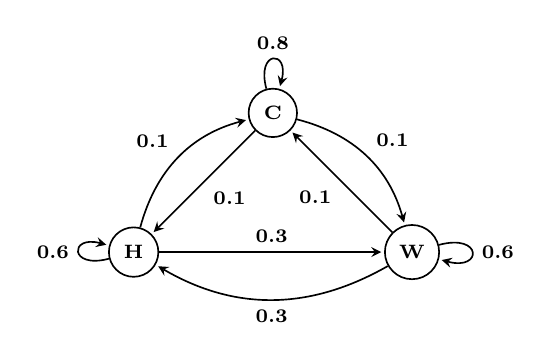
\begin{tikzpicture}[
		> = stealth, % arrow head style
		shorten > = 1pt, % don't touch arrow head to node
		auto,
		node distance = 2.5cm, % distance between nodes
		semithick, % line style
		font=\scriptsize\bfseries
		]
		
		\node[circle,draw] (qC) {C};
		\node[circle,draw] (qH) [below left of=qC] {H};
		\node[circle,draw] (qW) [below right of=qC] {W};
		
		\path[->] 	
		(qC) 	edge [loop above] node {0.8} ()
		edge [] node {0.1} (qH)
		edge [bend left] node {0.1} (qW)
		(qH) 	edge [loop left] node {0.6} ()
		edge [bend left] node {0.1} (qC)
		edge [] node {0.3} (qW)
		(qW)	edge [loop right] node {0.6} ()
		edge [bend left] node {0.3} (qH)
		edge [] node {0.1} (qC);
	\end{tikzpicture}
	\caption[Example of a Markov chain for weather prediction.]{Example of a Markov chain for weather prediction; figure reconstructed from \cite{2019-jurafsky-martin}.}
	\label{fig:cm-exp}
\end{figure}


%\begin{figure}[ht]
%	\centering
%	\hgraphpage[.4\textwidth]{exp-markov_.pdf}
%	\caption[Exemple d'un chaîne de Markov pour la prédiction du temps]{Exemple d'un chaîne de Markov pour la prédiction du temps \cite{2019-jurafsky-martin}\label{fig:cm-exp}}
%\end{figure}

This is a language model that represents only transition probabilities. In this case, we can only represent the transition probability from one category to another. If we estimate the emission probability of a word in each state (label), we could estimate the labels using Bayes' theorem. This model is called the Hidden Markov Model (\ac{hmm}); the words in a sequence are observed, unlike the hidden categories that need to be estimated. Each label (category) $t_i$ is represented by a state $q_i$ in the set of states $Q = \{q_1, q_2, \ldots, q_n\}$. Transitions from one state to another following a Bigram model are represented by the transition matrix $A$. The initial distribution of probabilities for these states is denoted $\pi = [\pi_1, \pi_2, \ldots, \pi_n]$, where $\sum_i \pi_i = 1$. A word $w_i$ is represented as an observation in the sequence of observed events $O = o_1 o_2 \ldots o_T$. An observation $o_t$ can be generated in a state $q_i$ with observation probabilities (emission probabilities) $B = b_i(o_t)$. An example of an \ac{hmm} is illustrated in Figure \ref{fig:hmm-exp}. Transitions represent the probabilities of moving from one label to another. Emissions represent the probabilities of word occurrences in labels.
\begin{figure}[ht]
	\centering
	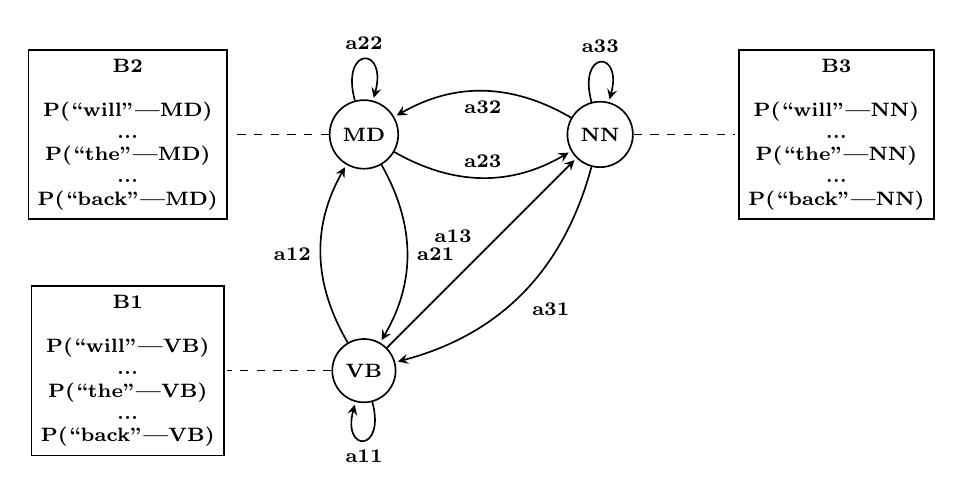
\begin{tikzpicture}[
		> = stealth, % arrow head style
		shorten > = 1pt, % don't touch arrow head to node
		auto,
		node distance = 3cm, % distance between nodes
		semithick, % line style
		font=\scriptsize\bfseries
		]
		
		\node[circle,draw] (q2) {MD};
		\node[align=center,draw] (q2e) [left of=q2] {B2\\ \\P(``will"|MD)\\...\\P(``the"|MD)\\...\\P(``back"|MD)};
		\node[circle,draw] (q3) [right of=q2] {NN};
		\node[align=center,draw] (q3e) [right of=q3] {B3\\ \\P(``will"|NN)\\...\\P(``the"|NN)\\...\\P(``back"|NN)};
		\node[circle,draw] (q1) [below of=q2] {VB};
		\node[align=center,draw] (q1e) [left of=q1] {B1\\ \\P(``will"|VB)\\...\\P(``the"|VB)\\...\\P(``back"|VB)};
		
		\path[->] 	
		(q1) 	edge [loop below] node {a11} ()
		edge [bend left] node {a12} (q2)
		edge [] node {a13} (q3)
		(q2) 	edge [loop above] node {a22} ()
		edge [bend left] node {a21} (q1)
		edge [bend right] node {a23} (q3)
		(q3)	edge [loop above] node {a33} ()
		edge [bend left] node {a31} (q1)
		edge [bend right] node {a32} (q2);
		
		\path[dashed] 	
		(q1) 	edge [] node {} (q1e)
		(q2) 	edge [] node {} (q2e)
		(q3) 	edge [] node {} (q3e);
		
	\end{tikzpicture}
	\caption[Example of HMM Representation]{Example of HMM Representation; figure reconstructed from \cite{2019-jurafsky-martin}.}
	\label{fig:hmm-exp}
\end{figure}

%\begin{figure}[ht]
%	\centering
%	\hgraphpage[.6\textwidth]{exp-hmm_.pdf}
%	\caption[Exemple d'une représentation HMM]{Exemple d'une représentation HMM \cite{2019-jurafsky-martin}\label{fig:hmm-exp}}
%\end{figure}

The estimated sequence $\hat{t}$ is the one that maximizes the probability $P(t)$ and the probability $P(w | t)$ according to Equation \ref{eq:hmm-detail}. Using a Bigram model, the probability $P(t)$ is calculated using transitions from the initial state $t_1$ to the last state $t_n$. It is important to note that the probability $P(t_1|t_0)$ is actually the initial probability $\pi_1$ of state $t_1$. The probability $P(w_i | t_i)$ is an emission probability in the Hidden Markov Model.

\begin{align}
	\hat{t} & = \arg\max\limits_t P(t) P(w | t) \nonumber\\
	& = \arg\max\limits_t P(t_1 \dots t_n) P(w_1 \dots w_n | t_1 \dots t_n) \nonumber\\
	& = \arg\max\limits_t \pi_{t1} \prod_{i=2}^{n} P(t_i|t_{i-1}) \prod_{i=1}^{n} P(w_i| t_i) \nonumber\\
	& = \arg\max\limits_t \prod_{i=1}^{n} \underbrace{P(t_i|t_{i-1})}_{a_{i-1,i}} \underbrace{P(w_i | t_i)}_{b_i(w_i)} \label{eq:hmm-detail}
\end{align}

Before discussing how a sequence $w=w_1 \ldots w_n$ is decoded according to Equation \ref{eq:hmm-detail}, we begin by describing training. In an \ac{hmm}, the states are the tags (categories) $t_i$, and the observations are the words $w_i$. Let the function that counts the occurrences of a sequence be denoted as $C$. The transition probability $a_{i-1,i}$ from state $t_{i-1}$ to $t_i$ is estimated from the training corpus according to Equation \ref{eq:pos-hmm1}. Note "<s>" is the label preceding the first category of the sentence. In this case, the probability $\pi_i$ of starting with state $t_i$ is estimated according to Equation \ref{eq:pos-hmm2}. The emission probability of a word $w_i$ in a state $t_i$ is estimated according to Equation \ref{eq:pos-hmm3}.

\begin{align}
	P(t_i | t_{i-1}) & = \frac{C(t_{i-1}, t_i)}{C(t_{i-1})}  \label{eq:pos-hmm1} \\
	\pi_i & = P(t_i | <s>) = \frac{C(<s>, t_i)}{C(<s>)} \label{eq:pos-hmm2} \\
	P(w_i | t_i) & = \frac{C(t_i, w_i)}{C(t_i)} \label{eq:pos-hmm3}
\end{align}

Let's take an example of a training corpus with four sentences and four categories: DT, PR, VB, and NM.

\begin{itemize}
	\item un/DT ordinateur/NM peut/VB vous/PR aider/VB
	\item il/PR veut/VB vous/PR aider/VB
	\item il/PR veut/VB un/DT ordinateur/NM
	\item il/PR peut/VB nager/VB
\end{itemize}

An example of calculating a transition is as follows: $P(VB | NM) = \frac{C(NM,\ VB)}{C(NM)} = \frac{1}{2}$. The emission probability of the word "veut" when the tag is "VB" is calculated as follows: $P(veut | VB) = \frac{C(VB,\ veut)}{C(VB)} = \frac{2}{7}$. The probability of a pronoun being at the beginning of the sentence is calculated as: $\pi_{PR} = \frac{C(<s>,\ PR)}{C(<s>)} = \frac{3}{4}$. The transition matrix as well as the initial distribution are illustrated in Table \ref{tab:hmm-trans-init}. Even though it is not used in the calculation, we added the transition from one state to the end to complete the distribution (to have a sum of 1 on the rows). Emission probabilities are illustrated in Table \ref{tab:hmm-emission}.

\begin{table}[ht]
	\centering\footnotesize
	\begin{tabular}{llllll}
		\cline{2-6}\noalign{\vskip\doublerulesep
			\vskip-\arrayrulewidth}\cline{2-6}
		& DT & PR & VB & NM & \textless/s\textgreater\\
		\hline
		DT  &  0  &  0   &  0   &   1  &  0  \\
		PR &  0  &  0   &   1  &  0   &  0  \\
		VB & 1/7 & 2/7  & 1/7  &  0   & 3/7 \\
		NM &  0  &  0   & 1/2  &   0  &  1/2 \\
		\hline
		\textless s\textgreater ($\pi$) &  1/4  &  3/4   & 0  &   0  &  0 \\
		\hline\hline
	\end{tabular}
	\caption[Example of transition probabilities and an initial distribution]{Example of transition probabilities and an initial distribution \label{tab:hmm-trans-init}}
\end{table}

\begin{table}[ht]
	\centering\footnotesize
	\begin{tabular}{lllllllll}
		\cline{2-9}\noalign{\vskip\doublerulesep
			\vskip-\arrayrulewidth}\cline{2-9}
		& un & ordinateur & peut & vous & aider & il & veut & nager \\
		\hline
		DT  &  1 &  0         &  0   &   0  &  0    & 0  & 0    & 0 \\
		PR &   0 &  0         &  0   & 1/4  &  0    &3/4 & 0    & 0 \\
		VB &   0 &  0         & 2/7  &   0  &  2/7  & 0  & 2/7  & 1/7 \\
		NM &   0 &  1         &  0   &   0  &  0    & 0  & 0    & 0 \\
		\hline\hline
	\end{tabular}
	\caption[Example of emission probabilities]{Example of emission probabilities \label{tab:hmm-emission}}
\end{table}

%\begin{figure}
%	\begin{tikzpicture}[
%	> = stealth, % arrow head style
%	shorten > = 1pt, % don't touch arrow head to node
%	auto,
%	node distance = 3cm, % distance between nodes
%	semithick, % line style
%	font=\small
%	]
%	
%	\tikzstyle{every state}=[
%	draw = black,
%	thick,
%	fill = white,
%	minimum size = 4mm
%	]
%	
%	\node[circle,draw] (qN) {N};
%	\node[align=left,draw] (qNe) [left of=qN] {P("fish"|N)=0.05\\P("river"|N)=0.03};
%	\node[circle,draw] (qV) [right of=qN] {V};
%	\node[align=left,draw] (qVe) [right of=qV] {P("fish"|V)=0.01\\P("eat"|V)=0.02};
%	\node[circle,draw] (qD) [below of=qN] {D};
%	\node[align=left,draw] (qDe) [left of=qD] {P("the"|D)=0.3\\P("a"|D)=0.2\\P("an"|D)=0.15};
%	\node[circle,draw] (qP) [right of=qD] {P};
%	\node[align=left,draw] (qPe) [right of=qP] {P("I"|P)=0.2\\P("he"|P)=0.1\\P("she"|P)=0.1};
%	\node[] () [below of=qD, yshift=1.5cm] {$\pi(P, D, V, N) = (0.4, 0.3, 0.1, 0.2)$};
%	
%	
%	\path[->] 	
%	(qN) 	edge [loop above] node {0.3} ()
%	edge [bend left] node {0.7} (qV)
%	(qV) 	edge [loop above] node {0.1} ()
%	edge [bend left] node {0.5} (qN)
%	edge [bend left] node {0.4} (qD)
%	(qD)	edge [bend left] node {1.0} (qN)
%	(qP)	edge [bend right] node {1.0} (qV);
%	
%	\path[dashed] 	
%	(qN) 	edge [] node {} (qNe)
%	(qV) 	edge [] node {} (qVe)
%	(qD) 	edge [] node {} (qDe)
%	(qP) 	edge [] node {} (qPe);
%	
%	\end{tikzpicture}
%	\caption{Exemple}
%\end{figure}

Now let's go back to the decoding of tags (tagging). After training a Hidden Markov Model $\lambda = (A, B)$, we want to use it to estimate the tag sequence $\hat{t} = \hat{t}_1 \hat{t}_2 \ldots \hat{t}_T$ from a sequence of observations (words) $w = w_1 w_2 \ldots w_T$ where we have $N$ possible tags. If we were to use a brute force decoding, we would have a complexity of $O(N^T)$. Since maximizing the tags for an observation (word) $w_t$ depends only on the tags of the previous observation, we can solve the search problem using dynamic programming. At each step $t$ of the sequence, we rely on the previous estimation to compute the probabilities of all tags in order to choose the one that maximizes the probability as the current estimation. We always need to save the previous state to go back at the end of the algorithm. This is called the \textbf{Viterbi} search (see Algorithm \ref{algo:viterbi}). In this case, the complexity is reduced to $O(N^2T)$, and the search remains exact.

\begin{algorithm}[ht]
	\KwData{$w = w_1 \ldots w_T$, HMM $\lambda = (A, B)$ with $N$ states}
	\KwResult{$best\_path$, $prob\_path$}
	
	Create two matrices $viterbi[N, T]$ and $backpointer[N, T]$\;
	
	\For{state $ s = 1 \ldots N$}{
		$viterbi[s, 1] = \pi_s * b_s(w_1);\, backpointer[s, 1] = 0$ \;
	}
	
	\For{$ t = 2 \ldots T$}{
		\For{state $ s = 1 \ldots N$}{
			$viterbi[s, t] = \max\limits_{s'=1}^N viterbi[s', t-1] * a_{s',s} * b_s(w_t)$\;
			$backpointer[s, t] = \arg\max\limits_{s'=1}^N viterbi[s', t-1] * a_{s',s} * b_s(w_t)$\;
		}
	}
	
	$prob\_path = \max\limits_{s=1}^N viterbi[s, T];\, pointer\_path = \arg\max\limits_{s=1}^N viterbi[s, T]$\;
	
	$best\_path$ is the path starting from $pointer\_path$ and following $backpointer$
	
	\Return $best\_path$, $prob\_path$\;
	\caption{Viterbi Algorithm for decoding a sequence according to a Hidden Markov Model.}
	\label{algo:viterbi}
\end{algorithm}

Using the trained model in the previous example, we want to find the tags for this sentence: \expword{il peut aider}. According to the Viterbi algorithm, we will have Table \ref{tab:hmm-viterbi-exp} where each cell is filled with calculations separated by semicolons (previous states) and the return pointer between square brackets. In the last sequence ("aider"), the state that maximizes the probability is "VB". The return is state 3 ("VB") with a return to state 2 ("PR"). Therefore, the annotated text is: \expword{il/PR peut/VB aider/VB}.


%\begin{table}[ht]
%	\centering\small
%	\begin{tabular}{llll}
%		\cline{2-4}\noalign{\vskip\doublerulesep
%			\vskip-\arrayrulewidth}\cline{2-4}
%		       & il & peut & aider \\
%		\hline
%		\multirow{4}{*}{DET}  &  \multirow{4}{*}{1/4 * 0}& 0 * 0 * 0 & 0 * 0 * 0 \\
%		  &  & 3/4 * 0 * 0 & 0 * 0 * 0\\
%		  &  & 0 * 1/7 * 0 & 6/28 * 1/7 * 0 \\
%		  &  & 0 * 0 * 0 & 0 * 0 * 0\\
%		\multirow{4}{*}{PRON} &  \multirow{4}{*}{3/4 * 1} &  0 * 0 * 0&  0 * 0 * 0\\
%		  &  & 3/4 * 0 * 0 & 0 * 0 * 0\\
%		  &  & 0 * 2/7 * 0 & 6/28 * 2/7 * 0\\
%		  &  & 0 * 0 * 0 & 0 * 0 * 0 \\
%		\multirow{4}{*}{VERB} &  \multirow{4}{*}{0 * 0} & 0 * 0 * 2/7 & 0 * 0 * 2/7 \\
%		  &  & 3/4 * 1 * 2/7 & 0 * 1 * 2/7 \\
%		  &  & 0 * 1/7 * 2/7 & 6/28 * 1/7 * 2/7\\
%		  &  & 0 * 1/2 * 2/7 & 0 * 1/7 * 2/7 \\
%		\multirow{4}{*}{NOUN} &  \multirow{4}{*}{0 * 0} & 0 * 1 * 0 & 0 * 1 * 0 \\
%		  &  & 3/4 * 0 * 0 & 6/28 * 0 * 0 \\
%		  &  & 0 * 0 * 0 & 0 * 0 * 0 \\
%		  &  & 0 * 0 * 0 & 0 * 0 * 0\\
%		\hline\hline
%	\end{tabular}
%	\caption{Un exemple des probabilités d'émission \label{tab:hmm-viterbi-exp}}
%\end{table}

\begin{table}[ht]
	\centering\footnotesize%\scriptsize
	\begin{tabular}{llll}
		\cline{2-4}\noalign{\vskip\doublerulesep
			\vskip-\arrayrulewidth}\cline{2-4}
		& il & peut & aider \\
		\hline
		DT  & $\frac{1}{4} * 0$ [0]& $0 * 0 * 0$; $\frac{3}{4} * 0 * 0$; $0 * \frac{1}{7} * 0$; $0 * 0 * 0$ [2] & $0 * 0 * 0$; $0 * 0 * 0$; $\frac{6}{28} * \frac{1}{7} * 0$; $0 * 0 * 0$ [3]\\
		PR & $\frac{3}{4} * 1$ [0]&  $0 * 0 * 0$; $\frac{3}{4} * 0 * 0$; $0 * \frac{2}{7} * 0$; $0 * 0 * 0$ [2]&  $0 * 0 * 0$; $0 * 0 * 0$; $\frac{6}{28} * \frac{2}{7} * 0$; $0 * 0 * 0$ [3]\\
		VB & $0 * 0$ [0]& $0 * 0 * \frac{2}{7}$; $\frac{3}{4} * 1 * \frac{2}{7}$; $0 * \frac{1}{7} * \frac{2}{7}$; $0 * \frac{1}{2} * \frac{2}{7}$ [2]& $0 * 0 * \frac{2}{7}$; $0 * 1 * \frac{2}{7}$; $\frac{6}{28} * \frac{1}{7} * \frac{2}{7}$; $0 * \frac{1}{7} * \frac{2}{7}$ [3]\\
		NM & $0 * 0$ [0]& $0 * 1 * 0$; $\frac{3}{4} * 0 * 0$; $0 * 0 * 0$; $0 * 0 * 0$ [1]& $0 * 1 * 0$; $\frac{6}{28} * 0 * 0$; $0 * 0 * 0$; $0 * 0 * 0$ [1]\\
		\hline\hline
	\end{tabular}
	\caption[Exemple d'exécution de l'algorithme de Viterbi]{Exemple d'exécution de l'algorithme de Viterbi \label{tab:hmm-viterbi-exp}}
\end{table}


%===================================================================================
\subsection{Maximum Entropy}
%===================================================================================

Estimates by Hidden Markov Models (\ac{hmm}) rely only on word statistics. It is difficult to introduce features such as suffixes, uppercase letters, etc. Logistic regression, which is a discriminative model, can combine several features to estimate an output probability. Unfortunately, this method does not take sequences into consideration. We can use features on the current word and the preceding words to estimate the label, as in Hidden Markov Models (\ac{hmm}). In this case, the model will be called a \acf{memm}. The problem comes down to maximizing the individual probabilities of each label $\hat{t}_i$ (see Equation \ref{eq:pos-emm-est}).
\begin{equation}\label{eq:pos-emm-est}
	\hat{t} = \arg\max\limits_t P(t | w) = \arg\max\limits_t \prod\limits_{i} P(t_i | w_i, t_{i-1})
\end{equation}
Let $s_i^j$ be the sequence $s_i \ldots s_j$. To estimate the label $t_i$ of a word $w_i$, we take $l$ previous words and $l$ subsequent words, in addition to $k$ previous tags. We use a set of features $f$ where $f_j$ can be the presence of uppercase letters in the word, etc. Using logistic regression, the problem will be formulated as in Equation \ref{eq:memm}. Learning aims to minimize the sum of multi-class labeling errors for each word (for each word, we will have several probabilities; one for each label).
\begin{equation}\label{eq:memm}
	\hat{t} = \arg\max\limits_t \prod\limits_{i}  
	\frac{exp\left(\sum_j \theta_j f_j(t_i, w_{i-l}^{i+l}, t_{i-k}^{i-1})\right)}%
	{\sum_{t' \in tags} exp\left(\sum_j \theta_j f_j(t'_i, w_{i-l}^{i+l}, t_{i-k}^{i-1})\right)}
\end{equation}

Here is a list of features $f$ that we can use in this method:
\begin{itemize}
	\item The word $w_i$ (considering each word as a feature)
	\item Previous tags
	\item $w_i$ contains a prefix from a list (\textit{len(prefix)} $\le 4$)
	\item $w_i$ contains a suffix from a list (\textit{len(suffix)} $\le 4$)
	\item $w_i$ contains a number
	\item $w_i$ contains an uppercase letter
	\item $w_i$ contains a hyphen
	\item $w_i$ is entirely in uppercase
	\item The shape of the word $w_i$ (Ex. \expword{X.X.X})
	\item $w_i$ is in uppercase with a hyphen and a number (Ex. \expword{CFC-12})
	\item $w_i$ is in uppercase followed by the words Co., Inc., etc. within 3 words maximum
\end{itemize}

\subsection{Neural network}

Recurrent Neural Networks (\ac{rnn}) are designed to process sequences. We have seen that an \ac{rnn} can be used as a language model by inputting the encoded word with \keyword[O]{One-Hot} and estimating the next word given the previous context. We modify the output: instead of the probabilities of words in the vocabulary, we try to estimate the probabilities of possible categories. Of course, we can use a hidden layer to learn a more compact representation of words in the input (\keyword[E]{embedding}). Figure \ref{fig:pos-rnn1} represents an example of a recurrent neural network for morpho-syntactic tag detection following this modification.
\begin{figure}[ht]
	\centering
	\hgraphpage[.6\textwidth]{rnn-simple.pdf}
	\caption[RNN simple pour l'étiquetage morpho-syntaxique.]{RNN simple pour l'étiquetage morpho-syntaxique.}
	\label{fig:pos-rnn1}
\end{figure}
%\begin{figure}[!ht]
%	\centering
%	\hgraphpage[.55\textwidth]{rnn-simple_.pdf}
%	\caption[RNN simple pour l'étiquetage morpho-syntaxique]{RNN simple pour l'étiquetage morpho-syntaxique \cite{2019-jurafsky-martin}\label{fig:pos-rnn1}}
%\end{figure}

If we wanted deeper and more complex networks, we could stack multiple \ac{rnn}s together. This allows the model to learn more complex processes, improving prediction. To train this model, we will need a large dataset; the size of this dataset increases with the number of stacked networks. Figure \ref{fig:pos-rnn2} illustrates a model with two stacked \ac{rnn}s.
\begin{figure}[ht]
	\centering
	\hgraphpage[.7\textwidth]{rnn-stack.pdf}
	\caption[RNNs empilés pour l'étiquetage morpho-syntaxique.]{RNNs empilés pour l'étiquetage morpho-syntaxique.}
	\label{fig:pos-rnn2}
\end{figure}
%\begin{figure}[!ht]
%	\centering
%	\hgraphpage[.55\textwidth]{rnn-stack_.pdf}
%	\caption[RNNs empilés pour l'étiquetage morpho-syntaxique]{RNNs empilés pour l'étiquetage morpho-syntaxique \cite{2019-jurafsky-martin}\label{fig:pos-rnn2}}
%\end{figure}

In the previous neural models, the current label $t_i$ depends on the current word $w_i$ and the past context. Sometimes, knowing the future context can improve the current decision; we can find a dependence between the current word and the words that follow. To estimate the current label based on the future context, we use a \ac{rnn} with a reversed sequence; that is, the label $t_i$ will depend on the sequence $w_n, w_{n-1}, \ldots, w_{i+1}, w_{i}$. To express bidirectionality, we use two \ac{rnn}s: forward $RNN_{forward}(w_1^i)$ and backward $RNN_{backward}(w_i^n)$. We calculate the sum between the two hidden states $h_i^f \oplus h_i^b$, resulting in a vector that must pass through a "softmax" function to estimate the tag probabilities. This architecture is illustrated in Figure \ref{fig:pos-rnn3}.
\begin{figure}[ht]
	\centering
	\hgraphpage[.7\textwidth]{rnn-bi.pdf}
	\caption[RNN bidirectionnel pour l'étiquetage morpho-syntaxique.]{RNN bidirectionnel pour l'étiquetage.}
	\label{fig:pos-rnn3}
\end{figure}
%\begin{figure}[!ht]
%	\centering
%	\hgraphpage[.60\textwidth]{rnn-bi_.pdf}
%	\caption[RNN bidirectionnel pour l'étiquetage morpho-syntaxique]{RNN bidirectionnel pour l'étiquetage morpho-syntaxique \cite{2019-jurafsky-martin}\label{fig:pos-rnn3}}
%\end{figure}

Languages are always evolving: adding new words, new forms, etc. In addition, we cannot capture all the variations of all words using a limited corpus, especially in strongly inflected languages. To represent the morphological variations of a word, we have to go down to the character level. An idea (see Figure \ref{fig:pos-rnn4}) is to use a character-level language model to encode a word and combine this code with the lexical code (\keyword[O]{One-Hot} or \keyword[E]{embedding}) of the word. The resulting code will be taken as the input of the recurrent network (simple, stacked, or bidirectional).
\begin{figure}[ht]
	\centering
	\hgraphpage[0.8\textwidth]{rnn-char.pdf}
	\caption[Embedding de caractères pour l'étiquetage morpho-syntaxique.]{RNN avec des embedding de caractères pour l'étiquetage morpho-syntaxique.}
	\label{fig:pos-rnn4}
\end{figure}
%\begin{figure}[ht]
%	\centering
%	\hgraphpage[0.5\textwidth]{rnn-char1_.pdf}
%	\hgraphpage[0.45\textwidth]{rnn-char2_.pdf}
%	\caption[Embedding de caractères pour l'étiquetage morpho-syntaxique]{RNN avec des embedding de caractères pour l'étiquetage morpho-syntaxique \cite{2019-jurafsky-martin}\label{fig:pos-rnn4}}
%\end{figure}

\sectioni{Discussion}
%\begin{discussion}
Every language must have a mechanism to identify entities existing in the world (plants, animals, cities, etc.) and the actions that an entity can perform (e.g., play, read, exist, etc.). Linguists differentiate between the function of a word in a sentence using categories. For example, a noun refers to an object (concrete or abstract), while an adjective is a word that represents a property of a noun. Therefore, knowing the category of a word aids in sentence comprehension. Automating the task of detecting the categories of a sequence of words is a step towards sentence understanding. Even in statistical tasks (which do not require understanding), word categories can be a good indicator.

Labeling words by their grammatical categories is a task belonging to sequence labeling tasks. Several approaches have been used to solve this problem: rule-based, statistical, and neural networks. Rule-based approaches are challenging to implement; a deep understanding of the treated language is required. This approach has been replaced by the statistical approach, which aims to estimate the label based on statistics on the current word as well as the previous words and their labels. With the advent of \acp{rnn}, this task has become easier; you just need a labeled corpus of sufficient size. In the architectures presented in this chapter, the input to an \ac{rnn} is a vector representation of the current word. In reality, we can define more complex architectures by introducing word features, such as the presence of suffixes. We can even encode all suffixes with One-Hot encoding and merge this code with the word code.

In this chapter, we presented sequence labeling, specifically morpho-syntactic labeling. We saw the approaches and some methods used to solve this task. But the question arises: how can we evaluate a sequence labeling system? Simply put, this task is a special case of classification: instead of classifying a sentence, we classify each word (or part) separately, taking into account their (temporal) interactions. Thus, classification evaluation metrics such as accuracy, recall, precision, etc., can be used. This concerns intrinsic evaluation, or we can evaluate the effect of this task on another (extrinsic evaluation).
%\end{discussion}


\section{Additional Resources}
%\begin{resources}

\subsubsection*{Exercises}

\begin{enumerate}
	\item Here is a hidden Markov model for morpho-syntactic tagging:
	
	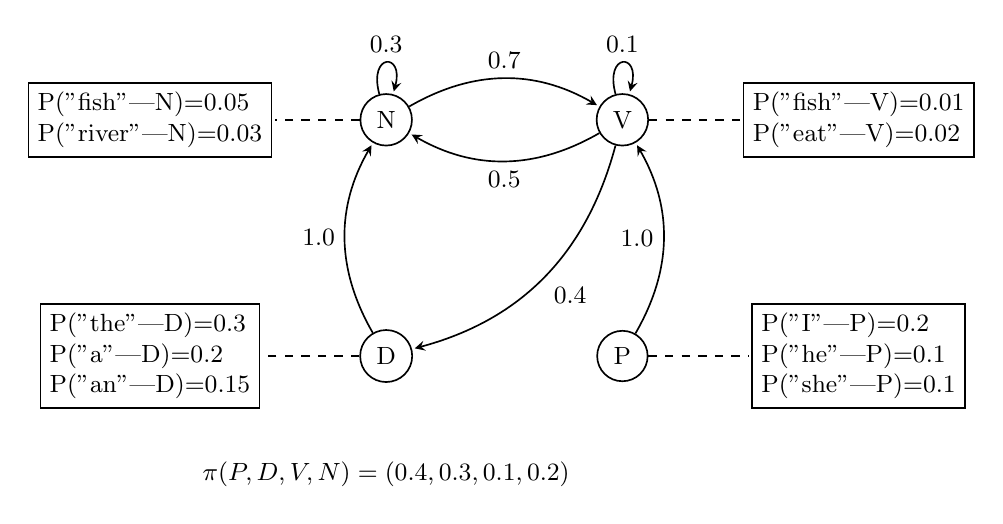
\begin{tikzpicture}[
		> = stealth, % arrow head style
		shorten > = 1pt, % don't touch arrow head to node
		auto,
		node distance = 3cm, % distance between nodes
		semithick, % line style
		font=\small
		]
		
		\tikzstyle{every state}=[
		draw = black,
		thick,
		fill = white,
		minimum size = 4mm
		]
		
		\node[circle,draw] (qN) {N};
		\node[align=left,draw] (qNe) [left of=qN] {P("fish"|N)=0.05\\P("river"|N)=0.03};
		\node[circle,draw] (qV) [right of=qN] {V};
		\node[align=left,draw] (qVe) [right of=qV] {P("fish"|V)=0.01\\P("eat"|V)=0.02};
		\node[circle,draw] (qD) [below of=qN] {D};
		\node[align=left,draw] (qDe) [left of=qD] {P("the"|D)=0.3\\P("a"|D)=0.2\\P("an"|D)=0.15};
		\node[circle,draw] (qP) [right of=qD] {P};
		\node[align=left,draw] (qPe) [right of=qP] {P("I"|P)=0.2\\P("he"|P)=0.1\\P("she"|P)=0.1};
		\node[] () [below of=qD, yshift=1.5cm] {$\pi(P, D, V, N) = (0.4, 0.3, 0.1, 0.2)$};
		
		\path[->] 	
		(qN) 	edge [loop above] node {0.3} ()
		edge [bend left] node {0.7} (qV)
		(qV) 	edge [loop above] node {0.1} ()
		edge [bend left] node {0.5} (qN)
		edge [bend left] node {0.4} (qD)
		(qD)	edge [bend left] node {1.0} (qN)
		(qP)	edge [bend right] node {1.0} (qV);
		
		\path[dashed] 	
		(qN) 	edge [] node {} (qNe)
		(qV) 	edge [] node {} (qVe)
		(qD) 	edge [] node {} (qDe)
		(qP) 	edge [] node {} (qPe);
		
	\end{tikzpicture}
	
	\begin{enumerate}
		\item Calculate the two probabilities: P(V D N | "fish a fish") and P(N D N | "fish a fish").
		\item Given that C(N) = 200, C(V) = 100, and C(D) = 100, calculate the following probabilities using Laplace smoothing: P(D|V), P(D|N), and P(N|D).
		\item Recalculate the probabilities from the first question after smoothing.
		\item How many expressions labeled "V D N" exist in our training dataset? The determinant "D" never occurs at the end of the sentence.
	\end{enumerate}
	
\end{enumerate}

%\end{resources}


\subsubsection*{Demos}

Demos are accessible via the Github repository.
In the first tutorial, we introduce the morpho-syntactic tagging task with NLTK, which is a Python-implemented tool for NLP. Several algorithms are used: RegEx, CRF, HMM, Perceptron, and Brill. We also present the named entity recognition task and the nominal phrase extraction task.

The second tutorial uses Flair, a Python tool for NLP. We cover both tasks: morpho-syntactic tagging and named entity recognition. In the tutorial, you can learn how to use an existing model and how to create a new one.

\subsubsection*{Lab: Morpho-syntactic Analysis}

We aim to design a small program for morpho-syntactic analysis from scratch. The HMM model with Laplace smoothing is provided. The student must implement the "Viterbi" decoding method.

The complete statement of the practical work along with the codes and data can be downloaded from the Github repository. The practical work is implemented entirely from scratch: the HMM module and the module that uses it for morpho-syntactic analysis. The student must complete two functions in the first module: scoring ($p(t_i|t_{i-1}, w_i)$) and Viterbi decoding. Two other decoding algorithms are implemented: brute force and greedy. The student must compare the three models by calculating the time complexity. The available programming languages (for now) are Java, Javascript/nodejs, and Python.


%\subsubsection*{Workshop}
%


%=====================================================================
\ifx\wholebook\relax\else
% \cleardoublepage
% \bibliographystyle{../use/ESIbib}
% \bibliography{../bib/RATstat}
	\end{document}
\fi
%=====================================================================


% !TEX TS-program = xelatex
% !TeX program = xelatex
% !TEX encoding = UTF-8
% !TeX spellcheck = en_US

%=====================================================================
\ifx\wholebook\relax\else
	\documentclass{KodeBook}
	\input{calls}
	\begin{document}
		\mainmatter
	
\fi
%=====================================================================
\changegraphpath{../img/parsing/}

\chapter{Parsing}

\begin{introduction}[NAT. LA\textcolor{white}{N}G. PROC.]
	\lettrine{N}{o} language can be understandable without a syntactic structure. 
	Let's take the phrase "Much to learn, you still have." as an example of analysis. 
	It is clear that the vocabulary is of English origin, but the sentence seems a bit unusual. 
	In English, sentences are often structured as subject-verb-object. 
	But in this sentence, the order is different: object-subject-verb; a structure similar to the indigenous languages of the Amazon. 
	Of course, in this case, it is the syntax used by Yoda (Star Wars). 
	There are several ways to view syntactic structure: a composition of structures until reaching an elementary structure, a set of relationships between words, etc. 
	In this chapter, we will present two syntactic structures and some parsing methods for both.
\end{introduction}

Syntax studies how words are combined to form a sentence. It seeks to define a standard structure for sentences in a language (natural or artificial). Syntactic analysis helps decide if a sentence is grammatically correct or not. If yes, we try to find its structure to assist in other tasks such as:
\begin{itemize}
	\item Detection of grammatical errors
	\item Language understanding
	\item Information extraction
\end{itemize}


%===================================================================================
\section{Syntactic Structures}
%===================================================================================

The sentences of a language must follow a syntactic structure based on construction rules.
In this section, we are interested in the formation of a grammatically correct sentence even if the meaning is erroneous.
%Here we are talking about a grammatically correct sentence; this does not mean that the sentence must make sense.
So, the fact that a sentence is well-formed syntactically is not a guarantee that it is semantically correct.
For example, the sentence "\expword{Les idées vertes et non colorées dorment furieusement.}" is syntactically well-formed but has no meaning.
There are several theories to represent syntactic structure:
\begin{itemize}
	\item Generative and transformational grammar
	\item Dependency grammar
	\item Categorial grammar
	\item Stochastic grammars
	\item Functional approaches to grammar
\end{itemize}


%===================================================================================
\subsection{Constituent Annotation}
%===================================================================================

In the previous chapter, we saw that each word in a language has a grammatical category (e.g., "\expword{Le/DET cours/NOM est/VP intéressant/ADJ}"). 
If we go back to the language models chapter, we can infer that the determinant has a high probability of being followed by a noun or an adjective followed by a noun (In RegEx: /\expword{DET ADJ* NOM}/). 
We call this structure a \keyword[S]{noun phrase (NP)}. 
It is called "noun" and not "adjectival" or "determiner" since the noun here is the center of the structure. 
The adjective often modifies a noun, and a determiner is always dependent on a noun. 
There are several \keywordpl[S]{phrase types} depending on the core category: nominal, verbal, adjectival, prepositional, etc. 
For example, \expword{[Le/DET cours/NOM ]\textsubscript{NP} [est/V intéressant/ADJ VP]\textsubscript{VP}}. 
The combination of several \keywordpl[S]{phrase types} forms another phrase until reaching the sentence. 
Technically, a sentence can be structured like a tree where the root is the sentence, phrases are represented by internal nodes, and words with their grammatical categories are represented by leaves.

Recall Chomsky's classification; a language can be: regular, context-free, context-sensitive, or recursively enumerable. 
Several languages can be formalized using a context-free grammar (CFG), e.g., in English. 
The grammar $G <\Sigma, N, P, S>$ of a language consists of:
\begin{itemize}
	\item $\Sigma$: set of terminal symbols; in this case, the vocabulary. 
	Example, \expword{$\Sigma$ = \{le, petit, chat, mange, un, poisson, ...\}}. 
	
	\item $N$: set of non-terminal symbols; variables (phrases and grammatical categories plus additional variables). 
	For example, \expword{$N$ = \{S, NP, VP, DET, N, ADJ, ...\}}.
	
	\item $S \in N$: axiom; it is the starting point for forming the sentence. 
	
	\item $P$: set of production rules.
	Rules are of the form $A \rightarrow \beta \text{ with } A \in N,\, \beta \in (\Sigma \cup N)^*$.
	For example, \expword{P=\{S \textrightarrow\ NP VP, NP \textrightarrow\ DET ADJ N \textbar\ DET N, VP \textrightarrow\ V NP\}}
\end{itemize}

Among the problems encountered during syntactic analysis is syntactic ambiguity. 
Let's take, for example, the following grammar (an ill-defined grammar):
\begin{itemize}
	\item S \textrightarrow\ NP VP (1)
	\item NP \textrightarrow\ DT NN (2) | DT NN PP (3)
	\item VP \textrightarrow\ VB NP (4) | VB NP PP (5)| VB PP (6) | AU VP (7)
	\item PP \textrightarrow\ PR NP (8)
	\item DT \textrightarrow\ l' | une | son 
	\item NN \textrightarrow\ élève | solution | stylo | explication 
	\item VB \textrightarrow\ écrit 
	\item AU \textrightarrow\ a
	\item PR \textrightarrow\ avec
\end{itemize}
According to this grammar, the sentence "\expword{L'élève a écrit une solution avec son explication}" has two interpretations. 
Both syntax trees are illustrated in Figure \ref{fig:cfg-ambigue}.
The first considers the preposition "avec" dependent on the noun "solution," and thus we have the following derivation (Figure \ref{fig:cfg-ambigue}(1)):
\begin{align*}
S & \sststile{}{(1)} NP\ VP \sststile{}{(2)} DT\ NN\ VP \sststile{}{(7)} DT\ NN\ AU\ VP \\
  & \sststile{}{(4)} DT\ NN\ AU\ VB\ NP \sststile{}{(3)} DT\ NN\ AU\ VB\ DT\ NN\ PP \\
  & \sststile{}{(8)} DT\ NN\ AU\ VB\ DT\ NN\ PR\ NP 
   \sststile{}{(2)} DT\ NN\ AU\ VB\ DT\ NN\ PR\ DT\ NN 
\end{align*}
La deuxième considère la préposition ``avec" dépendante du verbe ``écrit", et donc nous aurons la dérivation suivante (Figure \ref{fig:cfg-ambigue}(2)) :
\begin{align*}
S & \sststile{}{(1)} NP\ VP \sststile{}{(2)} DT\ NN\ VP \sststile{}{(7)} DT\ NN\ AU\ VP \\
& \sststile{}{(5)} DT\ NN\ AU\ VB\ NP\ PP \sststile{}{(2)} DT\ NN\ AU\ VB\ DT\ NN\ PP \\
& \sststile{}{(8)} DT\ NN\ AU\ VB\ DT\ NN\ PR\ NP 
 \sststile{}{(2)} DT\ NN\ AU\ VB\ DT\ NN\ PR\ DT\ NN 
\end{align*}
Clearly, there is ambiguity here; therefore, let's try to reformulate the two derivations.
The first means: the solution and its explanation have been written by the student. 
The second means: the solution has been written by the student using the explanation of the same student.
Clearly, the explanation is not a writing tool; therefore, the first one is more accurate. 
To resolve the ambiguity, we need semantic information that can guide the analysis. 
In our example, we can add the information that writing tools must be concrete entities and the object of writing must be an abstract entity.
\begin{figure}[ht]
	\begin{tabular}{cc}
		\hgraphpage[0.45\textwidth]{cfg-ambiguous1.pdf} &
		\hgraphpage[0.45\textwidth]{cfg-ambiguous2.pdf} \\
		(1) & (2) \\
	\end{tabular}
	\caption[Exemple de deux arbres syntaxiques d'une même phrase.]{Exemple de deux arbres syntaxiques de la phrase ``L'élève a écrit une solution avec son explication".}
	\label{fig:cfg-ambigue}
\end{figure}

Another method to deal with this problem is to use probabilistic context-free grammars (PCFG). 
The grammar is similar to that of a CFG: $G <\Sigma, N, P, S>$. 
The only difference is that the rules are of the form: $A \rightarrow \beta\, [p] \text{ with } A \in N,\, \beta \in (\Sigma \cup N)^*$.
We have only added the probability $p$ of the occurrence of the rule. 
To estimate this probability, we use an annotated corpus (TreeBank). 
Given the function $C$ that calculates the occurrence number, the probability of a rule $A \rightarrow \beta$ is estimated using Equation \ref{eq:pcfg-est}.
In the case of ambiguity between several rules, we choose the one with the maximum probability.
\begin{equation}\label{eq:pcfg-est}
	P(A \rightarrow \beta | A) = \frac{C(A \rightarrow \beta)}{C(A)}
\end{equation}


%===================================================================================
\subsection{Functional Annotation}
%===================================================================================

One or more words fulfill a syntactic function (e.g., \expword{subject, object, etc.}). 
For example, in the sentence "\expword{Le chat mange un poisson}" (The cat eats a fish), the word "\textit{chat}" (cat) is the subject of the verb "\textit{mange}" (eats). 
In functional annotation, the syntactic function is a binary relation called \keyword{dependency}.
A dependency relation connects a word called the \keyword{syntactic head} with another called the \keyword{dependent}. 
A word can be a dependent only once, but it can be a syntactic head several times. 
An example of the functional annotation of the two sentences "\expword{L'élève a écrit une solution et son explication}" (The student wrote a solution and its explanation) and "\expword{L'élève a écrit une solution avec son stylo}" (The student wrote a solution with his pen) is illustrated in Figure \ref{fig:parse-fct-exp}.
%
\begin{figure}[ht]
	\centering
	\hgraphpage[0.65\textwidth]{exp-parse-fonct2_.pdf}
	\caption[Example of functional analysis of two sentences.]{Example of functional analysis of two sentences using \url{https://corenlp.run/} [visited on 2022-05-18].}
	\label{fig:parse-fct-exp}
\end{figure}

The dependency structure is formalized as a directed graph $G=(V, A)$ where words are represented by vertices $V$, and relations are represented by arcs $A$. 
The dependency tree of a sentence satisfies the following conditions:
\begin{itemize}
	\item There is a single designated root node that has no incoming arcs. Generally, it is a verb.
	\item Except for the root node, each vertex has exactly one incoming arc.
	\item There is a unique path from the root node to each vertex in $V$.
\end{itemize}

Dependency relations are relations between two entities. 
An example of dependency relations is given in Table \ref{tab:rel-dep-exp}.
\begin{table}[ht]
	\begin{tabular}{p{.2\textwidth}p{.35\textwidth}p{.35\textwidth}}
		\hline\hline
		\textbf{Basic Dep.} & \textbf{Description} & \textbf{Example}\\
		\hline
		nsubj & nominal subject & \expword{Le \underline{people} \textbf{gagne}}\\
		obj & direct object & \expword{On \textbf{présente} le \underline{cours}}\\
		iobj & indirect object & \expword{Il \underline{m'}\textbf{envoie}}\\
		csubj & clausal subject & \expword{\underline{Suivre} le cours \textbf{permet} ...}\\
		&&\\
		\hline\hline
		\textbf{Nominal Dep.} & \textbf{Description} & \textbf{Example}\\
		\hline
		amod & adjectival modifier & \expword{La \textbf{fille} \underline{modeste}}\\
		det & determiner & \expword{\underline{La} \textbf{fille}}\\
		nmod & nominal modifier & \expword{Le \underline{résultat} de la \textbf{course}}\\
		nummod & numeric modifier & \expword{J'ai mangé \underline{3} \textbf{bonbons}}\\
		\hline\hline
	\end{tabular}
	\caption[Some universal Stanford dependency relations]{Some universal Stanford dependency relations \cite{2014-de-marneffe-al}, \url{https://universaldependencies.org/u/dep/index.html} [visited on 2021-09-11] }
	\label{tab:rel-dep-exp}
\end{table}


%===================================================================================
\subsection{Constituent Analysis}
%===================================================================================

Context-free grammar is the most commonly used formal system to model constituent structure.
There are two types of methods for analyzing a text:
\begin{itemize}
	\item \optword{bottom-up}: starting from the words of the sentence, we try to find the grammatical categories. Then, the phrases that generate a combination of categories and \keywordpl[S]{syntagme}. We merge the phrases until reaching the axiom "S".
	Example, \expword{LR}.
	\item \optword{top-down}: starting from the axiom "S", we look for the rules that generate the sentence. In this approach, we rely on the words to guide the generation.
	Example, \expword{Recursive Descent, LL, Early}.
\end{itemize}
The algorithms mentioned in the examples are designed to process programming languages. These have well-defined syntaxes that can be processed in a deterministic manner. Natural languages contain a lot of ambiguity, and the rules are more complex. An algorithm designed for natural language syntax parsing is the \keyword[C]{CKY} algorithm.

\subsection{CKY Algorithm}

The \keyword{Cocke-Kasami-Younger} (\keyword[C]{CKY}) algorithm uses dynamic programming to apply bottom-up syntactic analysis. The only condition to apply this algorithm is to transform the grammar $G <\Sigma, N, P, S>$ into Chomsky Normal Form (CNF). A brief reminder of this form ($N$ is the set of variables, and $\Sigma$ is the vocabulary):
\begin{align*}
	A & \rightarrow  B C \text{ where } A, B, C \in N\\
	A & \rightarrow w \text{ where } w \in \Sigma
\end{align*}

After transforming the grammar $G <\Sigma, N, P, S>$ into CNF, we can use it for phrase recognition. Given a sentence $w = w_1 \ldots w_n$, we create a triangular array $T$ of size $n*n/2$. Algorithm \ref{algo:cky-recon} describes how to fill this array to analyze the word $w$ following the grammar $G$ in CNF. The algorithm has been slightly modified to be able to go back and create the syntax tree: each cell contains a set of quadruplets (variable, index of the children, position of the first child, position of the second child). The algorithm takes time $O(n^3 * |P|)$ where $P$ is the set of productions. We start by filling the diagonal of the array $T$ with the variables $A$ that generate the words $w_i$ of the sentence $w$ ($A \rightarrow\ w_i$). We continue filling from bottom to top and from left to right. Each cell is filled by a variable that generates one of the variables to the left (column $k$) followed by one of the variables below (row $k$), where $i \le k \le j$. When we reach the last cell of the first row, we must find the axiom "S"; otherwise, the sentence does not belong to the language.

%\begin{algorithm}[ht]
%	\Donnees{une grammaire $G <\Sigma, N, P, S>$ en FNC; une phrase $w = w_1 \ldots w_n$}
%	\Res{$T[n, n], B[n, n, |N|]$}
%	
%	\Pour{$ i = 1 \ldots n$}{ %\tcc*{Iitialiser le diagonal}
%		$T[i, i] \leftarrow \{  A / (A \rightarrow w_i) \in P \} $\;
%	}
%	
%	\Pour{$ j = 2 \ldots n$ }{
%		\Pour{$ i = 0 \ldots (n - j) $}{
%			\Pour{$ k = (i+1) \ldots (i + j -1 ) $}{
%				\PourTous{$A$ tel que $(A \rightarrow B C) \in P $ et $B \in T[i, k]$ et $C \in T[k, i+j]$}{ 
%					$T[i, i+j] \leftarrow T[i, i+j] \cup \{A\}$ \;
%					$B[i, i+j, A] \leftarrow B[i, i+j, A] \cup \{(B, C, k)\}$ \;
%				}
%			}
%		}
%	}
%	
%	\Si{$``S" \notin T[0, n] $} {
%		Erreur ``La phrase n'a pas été reconnue"\;
%	}
%	
%	\Retour $T, B$ \;
%	\caption{Reconnaissance d'une phrase en utilisant la méthode CKY}
%	\label{algo:cky-recon}
%\end{algorithm}
\begin{algorithm}[ht]
	\Donnees{une grammaire $G <\Sigma, N, P, S>$ en FNC; une phrase $w = w_1 \ldots w_n$}
	\Res{$T[n, n]$}
	
	\Pour{$ i = 1 \ldots n$}{ %\tcc*{Initialiser le diagonal}
		$\selectfont T[i, i] \leftarrow \{ (A, 0, 0, 0) / (A \rightarrow w_i) \in P \}$\;
	}
	
	\Pour{$ i = (n-1) \ldots 1$ }{
		\Pour{$ j = (i+1) \ldots n $}{
			\Pour{$ k = i \ldots (j-1) $}{
				\PourTous{$A$ tel que $(A \rightarrow B C) \in P $ et $B \in T[i, k]$ et $C \in T[k+1, j]$}{
					$iB \leftarrow index(B, T[i, k])$ \;
					$iC \leftarrow index(C, T[k+1, j])$ \;
					$T[i, j] \leftarrow T[i, j] \cup \{(A, k, iB, iC)\}$ \;
				}
			}
		}
	}
	
	\Si{$``S" \notin T[1, n] $} {
		Erreur ``La phrase n'a pas été reconnue"\;
	}
	
	\caption{Reconnaissance d'une phrase en utilisant la méthode CKY}
	\label{algo:cky-recon}
\end{algorithm}

Once the sentence $w$ is accepted and the table is filled, we use the latter to generate the syntax tree.
We start by choosing the two children of the axiom $S$ based on $T$.
We look for the children of each node recursively until reaching a node without children.
Algorithm \ref{algo:cky-constr} describes the syntax tree construction operation in detail.
\begin{algorithm}[ht]
	\SetKwFunction{FConst}{Construire}
	\SetKwProg{Fn}{Fonction}{\\Début}{Fin}
	
	\Donnees{$T[n, n]$}
	\Res{Racine de l'arbre syntaxique : $r \leftarrow \varnothing$}
	
	\Si{$``S" \in T[1, n] $} {
		$r \leftarrow $ \FConst{$1, n, index(``S", T[1, n])$}\;
	}
	
	\Fn{\FConst{$i, j, pos$}}{
		$ (A, k, iB, iC) \leftarrow T[i, j][pos] $\;
		Créer un nouveau nœud : nœud\;
		nœud.valeur $\leftarrow  A$ \;
		\Si{$k>0$}{
			nœud.gauche $\leftarrow$ \FConst{$i, k, iB$}\;
			nœud.droit $\leftarrow$ \FConst{$k+1, j, iC$}\;
		}
		\Retour nœud\;
	}
	
	\caption{Construction de l'arbre syntaxique en utilisant CKY}
	\label{algo:cky-constr}
\end{algorithm}
%
%\begin{algorithm}[ht]
%	\SetKwFunction{FConst}{Construire}
%	\SetKwProg{Fn}{Fonction}{\\Début}{Fin}
%	
%	\Donnees{$T[n, n], B[n, n, |N|]$}
%	\Res{Arbre syntaxique}
%	
%	\eSi{$``S" \notin T[0, n] $} {
%		\Retour $\varnothing$ \;
%	}{
%		\Retour \FConst{$S, 0, n$}\;
%	}
%	
%	\Fn{\FConst{$A, i, j$}}{
%		
%		\eSi{j = i + 1}{
%			\Retour $A$\;
%		}{
%			$ (B, C, k) \leftarrow Choisir(B[i, j, A]) $\;
%			\Retour (\FConst{$B, i, k$}, \FConst{$C, k, j$})\;
%		}
%	}
%	
%	
%	\caption{Construction de l'arbre syntaxique en utilisant CKY}
%	\label{algo:cky-constr}
%\end{algorithm}

The resulting syntax tree is binary (due to Chomsky Normal Form).
However, in reality, it must follow the grammar designed by syntacticians.
One solution is to add a post-processing step to recover the original tree.
Regarding unit productions, we can leave them as they are and modify the \keyword[C]{CKY} algorithm to accept them.
Of course, the algorithm still suffers from the problem of syntactic ambiguity.
For example, "I eat rice with a fork" and "I eat rice with meat."

We will analyze the sentence "the little one forms a little sentence" using \keyword[C]{CKY} according to the following grammar:
\begin{itemize}
	\item S \textrightarrow\ NP VP | VP
	\item VP \textrightarrow V NP
	\item NP \textrightarrow\ \textbf{DET ADJ N} \textbar\ DET N \textbar\ PRON 
	\item PRON \textrightarrow\ I \textbar\ you \textbar\ he \textbar\ she
	\item V \textrightarrow\ forms \textbar\ wants \textbar\ eats 
	\item DET \textrightarrow\ a \textbar\ an \textbar\ the
	\item ADJ \textrightarrow\ little \textbar\ big \textbar\ blue 
	\item N \textrightarrow\ form \textbar\ sentence \textbar\ cat \textbar\ fish
\end{itemize}
We transform this grammar into CNF by replacing the bold rule with:
\begin{itemize}
	\item NP \textrightarrow\ DET AP
	\item AP \textrightarrow\ ADJ N
\end{itemize}
The unit rule "S \textrightarrow\ VP" will be replaced by "S \textrightarrow\ V NP."
The analysis table is illustrated in Figure \ref{fig:exp-cky-trait}.

\begin{figure}[ht]
\begin{tabular}{|p{2.3cm}|p{2.5cm}|p{2.3cm}|p{2.3cm}|p{2.5cm}|p{2.2cm}|}
	\hline
	la & petite & forme & une & petite & phrase \\
	\hline
	\textbf{(DET, 0, 0, 0)} & \textbf{(NP, 1, 1, 1)} & - & - & - & \textbf{(S, 2, 1, 1)} \\
	\hline
	\multicolumn{1}{l|}{}& \textbf{(ADJ, 0, 0, 0)}; (N, 0, 0, 0) & (AP, 2, 1, 2) & - & - & - \\
	\cline{2-6}
	\multicolumn{2}{l|}{}& \textbf{(V, 0, 0, 0)}; (N, 0, 0, 0) & - & (VP, 3, 1, 1) & \textbf{(VP, 3, 1, 1)}; (S, 3, 1, 1) \\
	\cline{3-6}
	\multicolumn{3}{l|}{}& \textbf{(DET, 0, 0, 0)} & (NP, 4, 1, 2) & \textbf{(NP, 4, 1, 1)} \\
	\cline{4-6}
	\multicolumn{4}{l|}{}& \textbf{(ADJ, 0, 0, 0)}; (N, 0, 0, 0) & \textbf{(AP, 5, 1, 1)} \\
	\cline{5-6}
	\multicolumn{5}{l|}{}& \textbf{(N, 0, 0, 0)} \\
	\cline{6-6}
\end{tabular}
\caption[Exemple de l'analyse CKY.]{Exemple de l'analyse CKY de la phrase ``la petite forme une petite phrase".}
\label{fig:exp-cky-trait}
\end{figure}


\subsection{Probabilistic CKY Algorithm}

In the \keyword[C]{CKY} algorithm, we may encounter a case where we have more than one syntax tree.
To guide the choice of rules, we add the probability of each production; using a \ac{pcfg}.
When transforming a probabilistic grammar $G<\Sigma, N, P, S>$ into CNF, the new rules created by transformation into CNF have a probability equal to $1$.
Given a syntax tree $T$ for the word $w$, its probability is estimated according to equation \ref{eq:pcfg-arbre-prop}.
\begin{equation}
	P(T, w) = \prod\limits_{(A_i \rightarrow \beta_i) \in T} P(A_i \rightarrow \beta_i)
	\label{eq:pcfg-arbre-prop}
\end{equation}
The most suitable syntax tree for analyzing the word $w$ is the one with the maximum probability (see \ref{eq:pcfg-arbre-max}).
\begin{equation}
	\hat{T}(w) = \arg\max\limits_{T(w)} P(T, w)
	\label{eq:pcfg-arbre-max}
\end{equation}

Regarding the \keyword[C]{CKY} algorithm, we add the probability of the occurrence of a rule in each cell.
Each variable $A$ will have at most one chance to produce two variables.
In this case, we create a three-dimensional triangular array $T[n, n, |N|]$ where we store the probability of each variable in that cell in addition to the position $k$ used to look for the children and the two variables of the left and right children.
We assume that all cell probabilities are initialized to $0$.
Algorithm \ref{algo:cky-prob-recon} represents the probabilistic version of the \keyword[C]{CKY} algorithm.
\begin{algorithm}[ht]
	\Donnees{une grammaire $G <\Sigma, N, P, S>$ en FNC; une phrase $w = w_1 \ldots w_n$}
	\Res{$T[n, n, |N|]$}
	
	\Pour{$ i = 1 \ldots n$}{ %\tcc*{Initialiser le diagonal}
		$T[i, i, A] \leftarrow \{ (P(A \rightarrow w_i), 0, A, A) / (A \rightarrow w_i) \in P \} $\;
	}
	
	\Pour{$ i = (n-1) \ldots 1$ }{
		\Pour{$ j = (i+1) \ldots n $}{
			\Pour{$ k = i \ldots (j-1) $}{
				\PourTous{$A$ tel que $(A \rightarrow B C) \in P $ et $T[i, k, B] > 0$ et $T[k+1, j, C] > 0$}{
					$p \leftarrow P(A \rightarrow B C) * T[i, k, B][1] * T[k+1, j, C][1]$\;
					\Si{$p > T[i, j, A][1]$}{
						$T[i, j, A] \leftarrow (p, k, B, C)$ \;
					}
				}
			}
		}
	}
	
	\Si{$T[1, n, S] = 0 $} {
		Erreur ``La phrase n'a pas été reconnue"\;
	}
	
	\caption{Reconnaissance d'une phrase en utilisant la méthode CKY probabiliste}
	\label{algo:cky-prob-recon}
\end{algorithm}
%\begin{algorithm}[ht]
%	\Donnees{une grammaire probabiliste $G <\Sigma, N, P, S>$ en FNC; une phrase $w = w_1 \ldots w_n$}
%	\Res{$T[n, n, |N|], B[n, n, |N|]$}
%	
%	\Pour{$ i = 1 \ldots n$}{ 
%		\PourTous{$A / (A \rightarrow w_j) \in P$}{
%			$T[i-1, j, A] \leftarrow P(A \rightarrow w_j)$\;
%		}
%	}
%	
%	\Pour{$ j = 2 \ldots n$ }{%\tcc*{Iitialiser le diagonal}
%		\Pour{$ i = 0 \ldots (n - j) $}{
%			\Pour{$ k = (i+1) \ldots (i + j -1 ) $}{
%				%					\PourTous{$A$ tel que $(A \rightarrow B C) \in P $ et $B \in T[i, k]$ et $C \in T[k, i+j]$}{ 
%				$T[i, i+j, A] \leftarrow \max\limits_{A \rightarrow B C \in P} P(A \rightarrow B C) * T[i, k, B] * T[k, i+j, C]$ \;
%				$B[i, i+j, A] \leftarrow (B, C, k)$\;
%				%					}
%			}
%		}
%	}
%	
%	\texttt{// Si $``S" \notin T[0, n] $ : Erreur}
%	%		\Si{} {
%	%			Erreur ``La phrase n'a pas été reconnue"\;
%	%		}
%	
%	\Retour $T, B$ \;
%	\caption{CKY probabiliste : Reconnaissance d'une phrase}
%\end{algorithm}

%===================================================================================
\section{Dependency Parsing}
%===================================================================================

Syntactic dependencies are binary relations between two words. Dependency parsing is used to find these relations and create a syntax tree. In this tree, all nodes are words, and each arc is a relation. We will present two approaches for dependency parsing: transition-based and graph-based.

\subsection{Transition-Based Approach}

A transition-based dependency parser can be implemented using the SHIFT-REDUCE method. It is an abstract machine with the configuration \(C = (\sigma, \beta, A)\) (see Figure \ref{fig:dep-trans-arch}), where:
\begin{itemize}
	\item \(\sigma\) is a stack.
	\item \(\beta\) is the input buffer. It contains the input word with a head pointing to the current word.
	\item \(A\) is the list of created arcs (dependencies).
\end{itemize}
The parsing starts with the initial configuration \(C_{initial} = ([ROOT], w, \emptyset)\) and finishes with the final configuration \(C_{final} = ([ROOT], \varnothing, A)\). If we reach the end of the word with a non-empty stack (here, we consider the \(ROOT\) as empty) without shift actions, we can conclude that the word does not belong to the language. A transition from one state to another can be an action on:
\begin{itemize}
	\item \(\sigma\): push or pop a word;
	\item \(\beta\): remove a word or add one at the beginning;
	\item \(A\): add a dependency between two words.
\end{itemize}
The \textbf{Oracle} is a trained model to decide the next transition.


\begin{figure}[ht]
	\centering
	\hgraphpage[.38\textwidth]{transitions.pdf}
	\caption{Architecture d'un analyseur des dépendances par transition.}
	\label{fig:dep-trans-arch}
\end{figure}


To describe the parsing algorithm, we use two functions: "$Oracle$" that chooses a transition "$t$", and "$Apply$" that executes "$t$" on the configuration. Algorithm \ref{algo:anal-dep-trans} describes the dependency parsing using transitions.

\begin{algorithm}[ht]
	\Donnees{Le mot à analyser $w= w_1 w_2 \ldots w_n$}
	\Res{Liste des dépendances $A$}
	
	$C \leftarrow (\sigma=[ROOT], \beta = w, A = \emptyset)$\;
	
	
	\Tq{$\sigma \ne [ROOT]$ OU $\beta \ne \varnothing$}{
		$t \leftarrow Oracle(C)$\;
		$C \leftarrow Appliquer(C, t)$\;
	}
	
	\caption{Analyse des dépendances par transitions \label{algo:anal-dep-trans}}
\end{algorithm}

The "Oracle" model chooses the next transition $\hat{t}$ from the set of possible transitions $T$. When we are in the current configuration $C = (\sigma, \beta, A)$, we use a function $\Psi$ that calculates a score using features based on this configuration. The chosen transition $\hat{t}$ is the one that maximizes the $\Psi$ function with parameters $\theta$ according to equation \ref{eq:orancle-psi}.
\begin{equation}\label{eq:orancle-psi}
	\hat{t} = \arg\max\limits_{t \in T} \Psi (t, C, w; \theta)
\end{equation}
To train the "Oracle" model, we need to annotate the text by transforming it into a sequence of transitions. The original text is annotated with dependency relations. To transform the output into a sequence of transitions, we use the parsing system to generate all possible dependencies. Using features on the current configuration, we try to estimate the next transition using the $\Psi$ function. This function can be MaxEnt (the most used), SVM, or neural networks. The features used by the $\Psi$ function can be features on:
\begin{itemize}
	\item the stack $\sigma$: the word on the top of the stack and its grammatical category.
	\item the input buffer $\beta$: the first three words and their grammatical categories.
	\item the list of dependencies $A$: the dependencies that have been estimated.
	\item the parsed sentence $w$: the distance between the word on the top of the stack and the first word in the buffer (number of words between them in the sentence $w$).
\end{itemize}

There are two approaches for dependency parsing by transitions: Arc-standard and Arc-eager. In Arc-standard, dependency relations are detected only between words in the stack. When a word is considered as the head of a relation, it will be popped from the stack. Table \ref{tab:arc-standard-exp} represents an example of parsing the sentence "Il écrit la solution et son explication" using Arc-standard. The possible transitions in this approach are:
\begin{itemize}
	\item \optword{SHIFT}: move the first element in the buffer to the stack
	\[ (\sigma, w_i|\beta, A) \Rightarrow  (\sigma|w_i, \beta, A) \]
	
	\item \optword{ARC-LEFT}: establish an arc from the first element in the buffer to the top of the stack
	\[ (\sigma|w_i, w_j|\beta, A) \Rightarrow  (\sigma, w_j|\beta, A \cup \{w_j \rightarrow w_i \}) \] 
	
	\item \optword{ARC-RIGHT}: establish an arc from the top of the stack to the first element in the buffer
	\[ (\sigma|w_i, w_j|\beta, A) \Rightarrow  (\sigma, w_i|\beta, A \cup \{w_i \rightarrow w_j \}) \] 
\end{itemize}


\begin{table}[ht]
	\centering\footnotesize
	\begin{tabular}{llll}
		\hline\hline
		nb. $\sigma$ (pile) & $\beta$ (tampon) & Action & Arc ajouté à A \\
		\hline
		01. [\textbf{ROOT}] & \textbf{Il} écrit la solution et son explication & SHIFT & / \\
		02. [ROOT, \textbf{Il}] & \textbf{écrit} la solution et son explication & ARC-LEFT & Il \textleftarrow\ écrit\\
		03. [\textbf{ROOT}] & \textbf{écrit} la solution et son explication & SHIFT & / \\
		04. [ROOT, \textbf{écrit}] & \textbf{la} solution et son explication & SHIFT & / \\
		05. [ROOT, écrit, \textbf{la}] & \textbf{solution} et son explication & SHIFT & / \\
		06. [ROOT, écrit, la, \textbf{solution}] & \textbf{et} son explication & SHIFT & / \\
		07. [ROOT, écrit, la, solution, \textbf{et}] & \textbf{son} explication & SHIFT & / \\
		08. [ROOT, écrit, la, solution, et, \textbf{son}] & \textbf{explication} & ARC-LEFT & son \textleftarrow\ explication\\
		09. [ROOT, écrit, la, solution, \textbf{et}] & \textbf{explication} & ARC-LEFT & et \textleftarrow\ explication\\
		10. [ROOT, écrit, la, \textbf{solution}] & \textbf{explication} & ARC-RIGHT & solution \textrightarrow\ explication\\
		11. [ROOT, écrit, \textbf{la}] & \textbf{solution} & ARC-LEFT & la \textleftarrow\ solution\\
		12. [ROOT, \textbf{écrit}] & \textbf{solution} & ARC-RIGHT & écrit \textrightarrow\ solution\\
		13. [\textbf{ROOT}] & \textbf{écrit} & ARC-RIGHT & ROOT \textrightarrow\ écrit\\
		14. [ROOT] & $\emptyset$ & FIN & / \\
		\hline\hline
	\end{tabular}
	\caption[Exemple de dérivations non étiquetées en utilisant Arc-standard.]{Exemple de dérivations non étiquetées de la phrase ``\expword{Il écrit la solution et son explication}" en utilisant Arc-standard.}
	\label{tab:arc-standard-exp}
\end{table}
%\begin{figure}[ht]
%	\centering
%	\hgraphpage[.8\textwidth]{exp-arc-std_.pdf}
%	\caption[Exemple de dérivations non étiquetées en utilisant Arc-standard]{Exemple de dérivations non étiquetées de la phrase ``\expword{they like bagels with lox}" en utilisant Arc-standard \cite{2018-eisenstein}\label{fig:arc-standard-exp}}
%\end{figure}

In Arc-Eager, we try to detect dependency relations as early as possible. To do this, relations must be detected between the top of the stack and the current word. In this case, we do not automatically advance the head of reading when we add a new relation. The only method to do this is to push the word onto the stack using the "SHIFT" transition. An example of parsing the sentence "Il écrit la solution et son explication" using Arc-eager is illustrated in Table \ref{tab:arc-eager-exp}. The possible transitions in this approach are:
\begin{itemize}
	\item \optword{SHIFT} is the same as "Arc-standard"
	
	\item \optword{ARC-LEFT}: establish an arc from the first element in the buffer to the top of the stack
	\[ (\sigma|w_i, w_j|\beta, A) \xRightarrow{\forall w_k (w_k \rightarrow w_i) \notin A}  (\sigma, w_j|\beta, A \cup \{w_j \rightarrow w_i \}) \] 
	
	\item \optword{ARC-RIGHT}: establish an arc from the top of the stack to the first element in the buffer
	\[ (\sigma|w_i, w_j|\beta, A) \Rightarrow  (\sigma|w_i w_j, \beta, A \cup \{w_i \rightarrow w_j \}) \] 
	
	\item \optword{REDUCE}: pop a word if it already has a parent
	\[ (\sigma|w_i, \beta, A) \xRightarrow{\exists w_k (w_k \rightarrow w_i) \in A} (\sigma, \beta, A) \] 
\end{itemize}


\begin{table}[ht]
		\centering\footnotesize
	\begin{tabular}{llll}
		\hline\hline
		nb. $\sigma$ (pile) & $\beta$ (tampon) & Action & Arc ajouté à A \\
		\hline
		01. [\textbf{ROOT}] & \textbf{Il} écrit la solution et son explication & SHIFT & / \\
		02. [ROOT, \textbf{Il}] & \textbf{écrit} la solution et son explication & ARC-LEFT & Il \textleftarrow\ écrit\\
		03. [\textbf{ROOT}] & \textbf{écrit} la solution et son explication & ARC-RIGHT & ROOT \textrightarrow\ écrit\\	
		04. [ROOT, \textbf{écrit}] & \textbf{la} solution et son explication & SHIFT & / \\	
		05. [ROOT, écrit, \textbf{la}] & \textbf{solution} et son explication & ARC-LEFT & la \textleftarrow\ solution \\
		06. [ROOT, \textbf{écrit}] & \textbf{solution} et son explication & ARC-RIGHT & écrit \textrightarrow\ solution \\
		07. [ROOT, écrit, \textbf{solution}] & \textbf{et} son explication & SHIFT & / \\
		08. [ROOT, écrit, solution, \textbf{et}] & \textbf{son} explication & SHIFT & / \\
		09. [ROOT, écrit, solution, et, \textbf{son}] & \textbf{explication} & ARC-LEFT & son \textleftarrow\ explication \\
		10. [ROOT, écrit, solution, \textbf{et}] & \textbf{explication} & ARC-LEFT & et \textleftarrow\ explication\\	
		11. [ROOT, écrit, \textbf{solution}] & \textbf{explication} & REDUCE & /\\
		12. [ROOT, \textbf{écrit}] & \textbf{solution} & ARC-RIGHT & écrit \textrightarrow\ solution\\
		13. [ROOT, \textbf{solution}] & $\emptyset$ & REDUCE & / \\
		14. [ROOT] & $\emptyset$ & FIN & / \\
		\hline\hline
	\end{tabular}
	\caption[Exemple de dérivations non étiquetées en utilisant Arc-eager.]{Exemple de dérivations non étiquetées de la phrase ``\expword{Il écrit la solution et son explication}" en utilisant Arc-eager.}
	\label{tab:arc-eager-exp}
\end{table}
%\begin{figure}[ht]
%	\centering
%	\hgraphpage[.8\textwidth]{exp-arc-eager_.pdf}
%	\caption[Exemple de dérivations non étiquetées en utilisant Arc-eager]{Exemple de dérivations non étiquetées de la phrase ``\expword{they like bagels with lox}" en utilisant Arc-eager \cite{2018-eisenstein}\label{fig:arc-eager-exp}}
%\end{figure}

The relations presented here are unlabeled relations; just the head-dependent relation without a type. To add the type of the relation, we need to enrich the "ARC-LEFT" and "ARC-RIGHT" transitions with the possible types. In Arc-standard, instead of 3 transitions, we will have $1+2R$ transitions where $R$ is the number of dependency types.


\subsection{Graph-based approach}

Filtering out non-probable relations is another approach to find the dependency tree of a given word $w$. Initially, we consider all possible dependencies between words. Then, we start eliminating non-probable relations until we reach the final result. Figure \ref{fig:dep-graph-arch} represents the general architecture of a graph-based dependency parser. The parser provides a "Notation" module that annotates the arcs.

Formally, we begin the analysis with a complete graph $G = (V, E)$ where $V$ is the set of nodes (words) and $E$ is the set of arcs (dependency relations). Then, we search for the tree $T = (V, F)$ among the possible trees $\mathcal{T}(G)$, which is a subgraph of $G$ maximizing a certain score, as indicated in Equation \ref{eq:arbre-rela-max}.
\begin{equation}
\hat{T} = \arg\max\limits_{T \in \mathcal{T}(G)} \Psi(T, w; \theta)
\label{eq:arbre-rela-max}
\end{equation}
The score $\Psi$ of a tree $T$ is the sum of the scores $\psi$ of its arcs (see Equation \ref{eq:arbre-rela-score}). 
Here, $\theta$ represents the set of parameters used in the scoring function.
\begin{equation}
\Psi(T, w; \theta) = \sum_{e \in F / T = (V, F)} \psi(e, w; \theta)
\label{eq:arbre-rela-score}
\end{equation}

\begin{figure}[ht]
	\centering
	\hgraphpage[.5\textwidth]{graph.pdf}
	\caption{Architecture d'un analyseur des dépendances par graphe.}
	\label{fig:dep-graph-arch}
\end{figure}

To estimate the score of an arc $e$, a set of features $f$ can be used, such as: the head word, its grammatical category, its lemma, its prefixes and suffixes, the direction of the arc, the distance between the head and the dependent, etc.
A learning algorithm with parameters $\theta$ is used to learn how to estimate the score of an arc $e$ based on these features.
Using initial scores, we generate a tree and compare it with the target tree.
If the trees are not identical, we calculate the error and update the parameters.
The score of an arc $e$ is represented by Equation \ref{eq:arbre-rela-score2}.
\begin{equation}
\psi(e, w; \theta) = \sum_{k = 1}^{K} \theta_k f_k(e, w)
\label{eq:arbre-rela-score2}
\end{equation}


To create a tree from a graph, the Chu-Liu/Edmonds algorithm can be used (see Algorithm \ref{algo:chu-liu-edmonds}).
To analyze a word $w=w_1 \ldots w_n$, we start by constructing a complete graph $G = (V, E)$ where each node $v_i$ represents a word $w_i$ and each arc $e$ represents a possible relationship between two nodes.
To represent the root word information, we add a node (ROOT) with arcs to all other nodes.
For each arc $e$ in the graph $G$, we assign a weight $G.p(e)$ that is estimated using machine learning.
Taking the node "ROOT" as the root and the graph $G$, we try to find a tree $T = (V, F)$ covering the maximum weight.
A covering tree is a maximal acyclic subgraph where all nodes are connected, and there is at most one incoming arc to a node.
Two functions are used in this algorithm:
\begin{itemize}
	\item \textbf{Contract}: a function that merges two nodes $u$ and $v$ forming a cycle $C$
	\begin{itemize}
		\item $\forall e = (u', v) \in E : G.p(e) \leftarrow G.p(e) - G.p((u, v)) $
		\item $\forall e = (v', u) \in E : G.p(e) \leftarrow G.p(e) - G.p((v, u)) $
	\end{itemize}
	\item \textbf{Extend}: a function that disassembles the two nodes $u$ and $v$ from a cycle $C$. The arc that violates the "no two incoming arcs" condition is removed.
\end{itemize}


\begin{algorithm}[ht]
	\Donnees{un graphe pondéré $G = (V, E)$, $ ROOT $}
	\Res{un arbre couvrant $T = (V, F)$}
	
	\SetKwFunction{ACM}{ArbreCouvrantMax}
	\SetKwProg{Fn}{Fonction}{}{Fin Fonction} 
	
	\Fn{\ACM{$G, ROOT$}}{
		
		$F \leftarrow \emptyset$\;
		
		\PourTous{$ v \in V$}{ 
			$meilleurInArc \leftarrow \arg\max_{e = (u, v) \in E} G.p(e) $;
			$F \leftarrow F \cup meilleurInArc$\;
			\PourTous{$e = (u, v) \in E$}{ 
				$ G.p(e) \leftarrow G.p(e) - G.p(meilleurInArc) $\;
			}
			\eSi{$T = (V, F)$ est un arbre couvrant}{
				\Retour $T$ \;
			}{
				$C \leftarrow$ un cycle de $F$;
				$G' \leftarrow Contracter(G, C)$\;
				$T' \leftarrow ArbreCouvrantMax(G', ROOT)$;
				$T \leftarrow Etendre(T', C)$\;
				\Retour $T$ \;
			}
		}
		
	}
	\caption{Analyse de Chu-Liu-Edmonds : Arbre couvrant de poids maximal\label{algo:chu-liu-edmonds}}
\end{algorithm}

Let's take the example of the sentence "\expword{Lisez le cours}".
Figure \ref{fig:cke-exp} represents its analysis using the Chu-Liu-Edmonds algorithm.
In the first graph, we looped three times to choose the arcs: (Root, Lisez), (le, cours), and (cours, le).
Each time an arc is chosen, we adjust the weight until we get the second graph.
Among the added arcs, there is a cycle \{(le, cours) and (cours, le)\}.
So, we need to merge the two nodes (contract) which gives us the third graph.
We apply the same operations to the resulting graph.
When there are no more cycles, we start extending the graph to remove unnecessary arcs.

\begin{figure}[ht]
	\centering
	\hgraphpage[.8\textwidth]{exp-graph-parsing.pdf}
	\caption[Exemple de l'analyse Chu-Liu-Edmonds]{Exemple de l'analyse de la phrase ``Lisez le cours" en utilisant l'algorithme de Chu-Liu-Edmonds ; figure inspirée de \cite{2019-jurafsky-martin}.}
	\label{fig:cke-exp}
\end{figure}

\sectioni{Discussion}
%\begin{discussion}
What is a language without syntax?
Try to imagine a people speaking a language (e.g., French) without using grammatical rules and only using vocabulary. 
No one would be able to understand each other. 
Certainly, we can have the elements of the sentence, but without structure, we cannot know their roles and relationships.

There are several theories of syntactic structure. 
Describing all these theories means writing an entire book just for syntax. 
We are interested in two main structures: constituent and functional.
The first one decomposes the sentence into phrases until it reaches a single word (a method used to teach language to primary school students). 
The second one tries to find binary syntactic relationships between words.

The most famous approach to represent constituents is context-free grammar. 
To analyze such a structure, we can use the CKY algorithm. 
This algorithm is improved by adding probabilities to the rules to have a deterministic analysis. 
There are methods that use more recent techniques like BERT (see the next chapter). 
To evaluate an automatic analysis, we can use the number of sentences with correct syntactic trees. 
This measure cannot differentiate between two erroneous syntactic trees; one of them may be more accurate than the other.

Dependency analysis can be accomplished by considering relationships as transitions and thus using a stack automaton to detect them.
Another approach is to consider all possible relationships and use graph properties to find a syntactic tree. 
The latter approach is more suitable for long-term relationships; when the sentence is too long.
In the case of dependencies, we can evaluate a tree by using the number of correct relationships.
%\end{discussion}



\section{Additional Resources}

\subsubsection*{Exercises}

\begin{enumerate}
	\item Here is a grammar (phrases and lexicon):
	
	\begin{tabular}{|lllll|}
		\hline
		S \textrightarrow\ NP VP & NP \textrightarrow\ DET N && DET \textrightarrow\ le | la & NN \textrightarrow\ Toma | Jerry \\
		NP \textrightarrow\ NN & VP \textrightarrow\ VT NP &&  N \textrightarrow\  souris | chat | fromage | maison & P \textrightarrow\ de\\
		VP \textrightarrow\ VI & PP \textrightarrow\ P NP && VT \textrightarrow\ mange | vole & VI \textrightarrow\ dort | sort\\
		\hline
	\end{tabular}
	
	\begin{enumerate}
		\item Add rules to generate the following sentences: (1) Le chat dors (2) La souris mange le fromage (3) Tom vole le fromage de la souris (4) Tom sort de la maison.
		\item Why are proper nouns separated from the set of nouns?
		\item We want to be able to generate the sentence: Nora vole le fromage du chat. The grammar should not generate a sentence like: Jerry vole la fromage de le chat. What rules should be added and removed? (In French: "de le" becomes "du".)
	\end{enumerate}
	
	\item Here is a grammar (phrases and lexicon):
	
	\begin{tabular}{|lllll|}
		\hline
		S \textrightarrow\ NP VP & NP \textrightarrow\ AJ NM | NM | PN & AJ \textrightarrow\ small | big  & VB \textrightarrow\ fish | like | swim &  \\
		PP \textrightarrow\ PR NP & VP \textrightarrow\ VB NP | VB PP & NM \textrightarrow\ fish | ducks & PR \textrightarrow\ like & PN \textrightarrow\ I \\
		\hline
	\end{tabular}
	
	\begin{enumerate}
		\item Analyze and draw the syntax tree for the sentences "big ducks like small fish," "I fish like big ducks," and "I swim like fish swim" using CKY.
		\item Analyze and draw the syntax tree for the same sentences using Arc-standard and Arc-Eager, where the choice is assumed to be perfect.
	\end{enumerate}
	
	\item Here is a treebank (4 sentences where each word is annotated with its grammatical category):
	
	\begin{tabular}{|lll|}
		\hline
		I/PN fish/VB small/AJ fish/NM &&
		I/PN swim/VB like/PR fish/NM\\
		ducks/NM swim/VB &&
		I/PN like/VB big/AJ fish/NM \\
		\hline
	\end{tabular}
	
	\begin{enumerate}
		\item Calculate the probability of each rule from the previous exercise.
		\item Analyze the sentences using probabilistic CKY.
		\item Analyze the 4 sentences with Arc-standard.
		\item Train a regression model that decides the next action (3 classes) based on the word and tag (a vector of 12 integers: 5 tags + 7 words). To simplify the calculation: apply only 5 iterations; use normalization instead of Softmax as the activation function; use the cost function without the "log" part.
	\end{enumerate}
	
	\item Suppose we have a word encoding model as follows: $Em(w_1\dots w_n) = \frac{\sum_{i=1}^{n} Pos(w_i)}{n}$ where $Pos$ is the position of the character in the alphabet. A model $Et$ for encoding tags involves ordering the tags alphabetically and returning the order of the tag as the code. Suppose we have trained a link scoring model where $Notation((u, v)) = \frac{Et(u) - Et(v)}{1+ Em(u)*Em(v)}$. We take $Em(Root) = 0$ and $Et(Root) = 0$. Analyze the dependencies of the sentence "ducks like fish" using the graph-based method.
\end{enumerate}


\subsubsection*{Demos}

Demos are accessible via the Github repository. In the first tutorial, Stanford CoreNLP is used to syntactically analyze two sentences. Two types of syntactic analysis are employed: constituency analysis and dependency analysis. It is worth mentioning that CoreNLP is a Java-based tool designed for Natural Language Processing.

The second tutorial utilizes NLTK, a well-known Python-based tool for Natural Language Processing. In this tutorial, various operations on Context-Free Grammars (CFG) are applied. It demonstrates how to create a new CFG, load it from a file, and use treebanks. Different constituency parsing algorithms and text generation are also tested.

\subsubsection*{Lab: CKY Syntactic Analysis}

The goal is to design a small program for syntactic analysis from scratch. Students must implement the CKY algorithm as discussed in the course.

The complete lab statement along with codes and data can be downloaded from the Github repository. The lab is implemented entirely from scratch: the CKY module and the module that utilizes it for morphosyntactic analysis. Students are required to implement the "analyze" function in the first module. The available programming languages (for now) are Java, Javascript/nodejs, and Python.


%\subsubsection*{Lab}
%
%Dans la tâche du "Jugements d'acceptabilité", on essaye de deviner si une phrase est acceptable grammaticalement. 
%Par exemple, l'expression "\textbf{Le livre qu'ont puisse trouvé sur internet ...}" ne peut pas être considérée comme acceptable. 
%La raison est que le verbe "ont (avoir)" est moins probable de suivre "que" et que le verbe "puisse (pouvoir)" est conjugué en présent subjonctif, or il est plus probable d'être en infinitif s'il suit le verbe "avoir".
%Dans ce lab, on va essayé de tester des différents modèles de langages afin d'accomplir cette tâche.
%
%L'énoncé complet du lab est téléchargeable à partir du répertoire Github.
%Les outils utilisés sont NLTK et Keras.le{../use/ESIbib}
% \bibliography{../bib/RATstat}


%=====================================================================
\ifx\wholebook\relax\else
% \cleardoublepage
% \bibliographysty\subsubsection*{Tutoriels}
	\end{document}
\fi
%=====================================================================


% !TEX TS-program = xelatex
% !TeX program = xelatex
% !TEX encoding = UTF-8
% !TeX spellcheck = en_US

%=====================================================================
\ifx\wholebook\relax\else
	\documentclass{KBook}
	\input{calls}
	\begin{document}
		\mainmatter
	
\fi
%=====================================================================
\changegraphpath{../img/word-sem/}

\chapter{Word Semantics}

\begin{introduction}[NAT. LAN\textcolor{white}{G}. PROC.]
	\lettrine{G}{enerally}, we can understand a text by using the meaning of each word that composes it. One day someone decided to invent metaphors, resulting in the phenomenon of polysemy; a word with multiple meanings. Since that day, humans have become lost! To process words automatically, we need to encode them. There are two representations: based on semantic relations with other words or using a vector representation. In the first representation, polysemous words can have different codes depending on their meanings. In vector representation, we need to choose whether to represent a word by a single vector regardless of its meaning or to use a more advanced representation based on context (neighboring words). In this chapter, we will present both approaches: lexical databases and vector representation.
\end{introduction}

A word, as a unit of text processing, needs to be encoded to facilitate tasks applied to the text. Information is encoded in the human brain using a phenomenon called long-term potentiation. This is the perspective of the physiological approach. As for the mental approach, among the types of encoding, we can mention visual encoding. In this case, the mental representation of a word has no relation to the language spoken by the individual. For example, the words "\<sajaraT> /shajarah/" in Arabic, "tree" in English, "arbre" in French, and "木 /ki/" in Japanese all refer to the same concept: an object with a trunk on which branches branch out bearing foliage. In computer science, representing concepts using images increases storage size and processing time. Instead, we use a less costly encoding such as relations with other concepts or a vector of numbers. A representation is better when it can deal with ambiguity. Take three sentences in French that contain the word "café" but with three different meanings:
\begin{itemize}
	\item \expword{Je veux boire du café.}
	\item \expword{Je veux aller au café.}
	\item \expword{Je veux récolter du café.}
\end{itemize}
The word "café" in this case will not have the same mental representation. In the first sentence, this word represents a liquid; unless we can imagine someone drinking a solid substance (coffee beans). In the second sentence, the word "café" represents a place; we cannot go to a liquid unless we consider it as a place. When talking about a place, it is common to consider the cafeteria and not the place where a glass of coffee is located. The last sentence uses the word "café" as a product harvested from the earth.

In summary, the motivation of this chapter is to present the different methods of encoding words, focusing on the semantic level. The first approach uses lexical semantics. This involves studying the meaning of words, such as classifying words based on meanings and the relationships between different meanings. The second approach uses statistical semantics. It applies statistical methods, such as unsupervised learning, to determine the meanings of words. The meanings of words can vary; the essential thing is to ensure sufficient accuracy, at least for information retrieval.

%===================================================================================
\section{Lexical Databases}
%===================================================================================

A lexical database is a database containing the vocabulary of a language. In addition to the vocabulary, it provides information about each word: grammatical category, lemma, frequency, etc. This information is linked by relations. Figure \ref{fig:base-lex-exp} represents a lexical database. A word is part of a lexeme, which is represented by one and only one lemma. A lexeme can represent multiple senses; which are referenced here by Synset and defined by a glossary.
 
\begin{figure}[ht]
	\centering 
	\hgraphpage[.6\textwidth]{exp-bd-lex.pdf}
	\caption[Exemple des informations et leurs relations dans une base lexicale.]{Exemple des informations et leurs relations dans une base lexicale ; figure reconstruite de \cite{2019-white-al}.}
	\label{fig:base-lex-exp}
\end{figure}

%===================================================================================
\subsection{Semantic Relations}

Let's recall the semantic relations presented in the first chapter:
\begin{itemize}
	\item \optword{Synonymy}: having similar meanings in a given context
	\item \optword{Antonymy}: having opposite meanings in a given context
	\item Taxonomic relations (classification)
	\begin{itemize}
		\item \optword{Hyponymy}: being more specific than another sense. It entails an \keyword{IS-A} relation. Ex. "car IS-A vehicle".
		\item \optword{Hyperonymy}: being more generic than another sense.
		\item \optword{Meronymy}: being a part of something. Ex. "wheel is a meronym of car; car is the holonym of wheel".
	\end{itemize}
\end{itemize}

\subsection{WordNet}

\keyword{WordNet} \cite{1995-miller} is a lexical database for English.
Figure \ref{fig:wordnet-exp} shows an example of the different senses of the word "reason". The database contains three parts: (1) nouns (2) verbs (3) adjectives and adverbs. A sense groups several words of the same part, and it is represented by an identifier called \keyword{Synset} (Synonyms set). For example, \expword{05659525 : reason\#3, understanding\#4, intellect\#2}. A sense is defined by a glossary (\keyword{Gloss}). For example, \expword{05659525 : (the capacity for rational thought or inference or discrimination) "we are told that man is endowed with reason and capable of distinguishing good from evil"}.

\begin{figure}[ht]
	\centering
	\begin{tcolorbox}[colback=white, colframe=blue, boxrule=1pt, text width=.90\textwidth]
%		\footnotesize
		\fontsize{11}{8}\selectfont
%		\begin{alltt}
			{\normalsize\bfseries Noun}
			\begin{itemize}[label=$\bullet$]
				\item \textcolor{blue}{\underline{S:}} \textcolor{red}{(n)} \textbf{reason}, \textcolor{blue}{\underline{ground}} (a rational motive for a belief or action) \textit{"the reason that war was declared"; "the grounds for their declaration"}
				\item \textcolor{blue}{\underline{S:}} \textcolor{red}{(n)} \textbf{reason} (an explanation of the cause of some phenomenon) \textit{"the reason a steady state was never reached was that the back pressure built up too slowly"}
				\item \textcolor{blue}{\underline{S:}} \textcolor{red}{(n)} \textbf{reason}, \textcolor{blue}{\underline{understanding}}, \textcolor{blue}{\underline{intellect}} (the capacity for rational thought or inference or discrimination) \textit{"we are told that man is endowed with reason and capable of distinguishing good from evil"}
				\item \textcolor{blue}{\underline{S:}} \textcolor{red}{(n)} \textcolor{blue}{\underline{rationality}}, \textbf{reason}, \textcolor{blue}{\underline{reasonableness}} (the state of having good sense and sound judgment) \textit{"his rationality may have been impaired"; "he had to rely less on reason than on rousing their emotions"}
				\item \textcolor{blue}{\underline{S:}} \textcolor{red}{(n)} \textcolor{blue}{\underline{cause}}, \textbf{reason}, \textcolor{blue}{\underline{grounds}} (a justification for something existing or happening) \textit{"he had no cause to complain"; "they had good reason to rejoice"}
				\item \textcolor{blue}{\underline{S:}} \textcolor{red}{(n)} \textbf{reason} (a fact that logically justifies some premise or conclusion) \textit{"there is reason to believe he is lying"}
			\end{itemize}
			
			{\normalsize\bfseries Verb}
			\begin{itemize}[label=$\bullet$]
				\item \textcolor{blue}{\underline{S:}} \textcolor{red}{(v)} \textbf{reason}, \textcolor{blue}{\underline{reason out}}, \textcolor{blue}{\underline{conclude}} (decide by reasoning; draw or come to a conclusion) \textit{"We reasoned that it was cheaper to rent than to buy a house"}
				\item \textcolor{blue}{\underline{S:}} \textcolor{red}{(v)} \textcolor{blue}{\underline{argue}}, \textbf{reason} (present reasons and arguments)
				\item \textcolor{blue}{\underline{S:}} \textcolor{red}{(v)} \textbf{reason} (think logically) \textit{"The children must learn to reason"}
			\end{itemize}
%		\end{alltt}
	\end{tcolorbox}
	\caption[Exemple de WordNet.]{Exemple de WordNet généré par \url{http://wordnetweb.princeton.edu/perl/webwn} [visité le 2022-05-01].}
	\label{fig:wordnet-exp}
\end{figure}

%\begin{figure}[ht]
%	\centering
%	\hgraphpage[.7\textwidth]{exp-wordnet_.pdf}
%	\caption[Exemple de WordNet]{Exemple de WordNet généré par \url{http://wordnetweb.princeton.edu/perl/webwn}}
%	\label{fig:wordnet-exp}
%\end{figure}

A sense is marked by a lexicographic category (\keyword{supersense}). 
Example. \expword{05659525: noun.cognition}
Table \ref{tab:cat-lex-wordnet} represents the lexicographic categories used in WordNet.

\begin{table}[ht]
	\centering\small
	\begin{tabular}{llllll}
		\hline\hline
		\textbf{Catégorie} & \textbf{Exemple} & \textbf{Catégorie} & \textbf{Exemple} &\textbf{Catégorie} & \textbf{Exemple} \\
		\hline
		ACT & service & GROUP & place & PLANT & tree \\
		ANIMAL &  dog & LOCATION & area & POSSESSION & price \\
		ARTIFACT & car & MOTIVE & reason & PROCESS & process \\
		ATTRIBUTE & quality & NATURAL EVENT & experience & QUANTITY & amount \\
		BODY & hair & NATURAL OBJECT & flower & RELATION & portion \\
		COGNITION & way & OTHER & stuff & SHAPE & square\\
		COMMUNICATION & review & PERSON & people & STATE & pain\\
		FEELING & discomfort & PHENOMENON & result & SUBSTANCE & oil \\
		FOOD & food & & & TIME & day\\
		\hline\hline
	\end{tabular}
	\caption[Catégories lexicographiques des noms dans WordNet]{Catégories lexicographiques des noms dans WordNet \cite{2019-jurafsky-martin}}
	\label{tab:cat-lex-wordnet}
\end{table}
%\begin{figure}
%	\hgraphpage{wordnet-supersenses_.pdf}
%	\caption{Les catégories lexicographiques des noms dans WordNet \cite{2019-jurafsky-martin}}
%\end{figure}

\keyword[W]{WordNet} represents the semantic relations between senses.
Table \ref{tab:rel-sem-wordnet} represents the semantic relations of nouns and verbs.

\begin{table}[ht]
	\small\centering
	\begin{tabular}{p{.2\textwidth}p{.45\textwidth}p{.25\textwidth}}
		\hline\hline
		\multicolumn{3}{c}{\textbf{Noms}}\\
		\hline
		\textbf{Relation} & \textbf{Définition} & \textbf{Exemple} \\
		\hline
		Hypernym & d'un concept spécifique vers un autre générique & \expword{breakfast\textsuperscript{1} \textrightarrow\ meal\textsuperscript{1} }\\
		Hyponym & d'un concept générique vers un autre spécifique & \expword{meal\textsuperscript{1} \textrightarrow\ lunch\textsuperscript{1}} \\
		Instance Hypernym & d'une instance vers son concept & \expword{Austen\textsuperscript{1} \textrightarrow\ author\textsuperscript{1}} \\
		Instance Hyponym & d'un concept vers son instance & \expword{composer\textsuperscript{1} \textrightarrow\ Bach\textsuperscript{1}} \\
		Part Meronym & d'un concept entier vers une partie & \expword{table\textsuperscript{2} \textrightarrow\ leg\textsuperscript{3}} \\
		Part Holonym & d'une partie vers un entier & \expword{course\textsuperscript{7} \textrightarrow\ meal\textsuperscript{1}} \\
		Antonym & d'un concept vers son opposition sémantique & \expword{leader\textsuperscript{1} $ \leftrightarrow $ follower\textsuperscript{1}}\\
		Derivation & d'un mot vers un autre ayant la même racine & \expword{destruction\textsuperscript{1} $ \leftrightarrow $ destroy\textsuperscript{1}} \\
		\hline\hline
		\multicolumn{3}{c}{\textbf{Verbes}}\\
		\hline
		\textbf{Relation} & \textbf{Définition} & \textbf{Exemple} \\
		\hline
		Hypernym & d'un évènement spécifique vers un autre générique & \expword{fly\textsuperscript{9} \textrightarrow\ travel\textsuperscript{5}} \\
		Troponym & d'un évènement générique vers un autre spécifique & \expword{walk\textsuperscript{1} \textrightarrow\ stroll\textsuperscript{1}} \\
		Entails & d'un évènement vers un autre qui l'implique & \expword{snore\textsuperscript{1} \textrightarrow\ sleep\textsuperscript{1}} \\ 
		Antonym & d'un évènement vers son opposition sémantique & \expword{increase\textsuperscript{1} $ \leftrightarrow $ decrease\textsuperscript{1}} \\
		\hline\hline
	\end{tabular}
	\caption[Relations sémantiques de Wordnet]{Relations sémantiques de Wordnet \cite{2019-jurafsky-martin}}
	\label{tab:rel-sem-wordnet}
\end{table}

%\begin{figure}
%	\hgraphpage{wordnet-rel-nom_.pdf}\vspace{-9pt}
%	\caption{Quelques relations des noms \cite{2019-jurafsky-martin}}
%\end{figure}\vspace{-6pt}
%
%\begin{figure}
%	\hgraphpage{wordnet-rel-verbe_.pdf}\vspace{-9pt}
%	\caption{Quelques relations des verbes \cite{2019-jurafsky-martin}}
%\end{figure}

There are projects to extend WordNet to other languages. 
Among these projects, we can mention: Global WordNet Association\footnote{Global WordNet Association: \url{http://globalwordnet.org/resources/wordnets-in-the-world/} [visited on 2021-09-11]} and Open Multilingual Wordnet\footnote{Open Multilingual Wordnet: \url{http://compling.hss.ntu.edu.sg/omw/} [visited on 2021-09-11]}.
To navigate Wordnet, there are several APIs. 
Here is a short list of these APIs:
\begin{itemize}
	\item NLTK (Python) : \url{https://www.nltk.org/howto/wordnet.html} [visité le 2021-09-25]
	\item JWI (Java) : \url{http://projects.csail.mit.edu/jwi} [visité le 2021-09-25]
	\item Wordnet (Ruby) : \url{https://github.com/wordnet/wordnet} [visité le 2021-09-25]
	\item OpenNlp (C\#) : \url{https://github.com/AlexPoint/OpenNlp} [visité le 2021-09-25]
\end{itemize}

\subsection{Other Resources}

\keyword[W]{WordNet} is not the only lexical database; there are others. 
VerbNet is another lexical database, but only for verbs. 
It includes 30 main thematic roles. 
Verbs are organized into classes. 
\keyword[F]{FrameNet} is another lexical database based on the sense theory called "semantic frame". 
A frame can be an event, a relation, or an entity with its participants. 
For example, the concept "\expword{Cook}" implies a person who cooks, food, a container, and a heat source.
Each frame is activated by a set of lexical units. 
For example, \expword{blanch, boil, grill, brown, simmer, cook}.
These two projects will be revisited in the next chapter (meaning of propositions).

Another project similar to Wordnet is BabelNet\footnote{BabelNet: \url{https://babelnet.org/} [visited on 2021-09-25]}.
It is a multilingual semantic network that uses several sources such as Wordnet, Wikipedia, VerbNet, etc. 
Each concept has a synset as in \keyword[W]{WordNet} and is shared by several languages. 
The structure of BabelNet is illustrated in Figure \ref{fig:babelnet-struc}.
\begin{figure}[ht]
	\hgraphpage{babelnet.pdf}
	\caption[Structure of BabelNet.]{Structure of BabelNet; figure reconstructed from \cite{2012-navigli-ponzetto}.}
	\label{fig:babelnet-struc}
\end{figure}


%===================================================================================
\section{Vector Representation of Words}
%===================================================================================

The simplest vector representation is the use of \keyword[O]{One-Hot} encoding. 
In this representation, we take a vector of size equal to the vocabulary size, and we choose a position to represent a given word. 
So, the word will be represented with a vector containing zeros except for the position reserved for it, where it will have a $1$. 
This representation is really costly in terms of size. 
Moreover, we cannot really represent a document or a sentence using this representation. 
This is because it does not represent the semantic relations between words: similarity (e.g., \expword{cat, dog}) and proximity (e.g., \expword{coffee, cup}). 

This representation can be used with machine learning algorithms like neural networks.
But there are other vector representations that are more informative. 
In this case, a term can be represented in relation to another reference such as: 
\begin{itemize}
	\item \optword{Term-document} : we represent a term by the documents that contain it (or vice versa).
	Example: \expword{\ac{tfidf}}.
	
	\item \optword{Term-term} : we represent a term by other terms.
	
	\item \optword{Term-concept-document} : we represent terms and documents by a vector of concepts.
	Example: \expword{Latent Semantic Analysis; \ac{lsa}}.
\end{itemize}


\subsection{TF-IDF}

The meaning of a document or a sentence can be represented by the words it contains and vice versa.
So, a document can be represented by the frequencies of occurrence of the words in the vocabulary. 
Similarly, a word can be represented by the frequencies of its occurrences in each document.
The frequency of a word in a document/sentence is called ``\ac{tf}".
It can be calculated by counting the number of occurrences of a term $t$ in a document $d$ as shown in Equation \ref{eq:tf}.
\begin{equation}
	TF_d(t) =  |\{t_i \in d / t_i = t\}|
	\label{eq:tf}
\end{equation}

In general, this representation is used in information retrieval tasks.
Sometimes, we want to give more weight to new words. 
This is motivated by the fact that words that are repeated too much in a specific domain do not have an added sense.
For example, the word ``\expword{computer}" will not be really important if the treated domain is computer science. 
It will be more beneficial to consider words that are more frequent in the document but are not as frequent in documents in the same domain.
To calculate the novelty of a term $t$, we use a set of documents $D$ in the same domain. 
Equation \ref{eq:idf} represents the method for calculating \ac{idf}.
\begin{equation}
	IDF_D(t) = \log_{10} \left( \frac{|\{d \in D\}|}{|\{d \in D / t \in d\}|} \right)
	\label{eq:idf}
\end{equation}
By multiplying the importance of the word $t$ in the document $d$ (\ac{tf}) by its novelty with respect to a set of documents $D$ (\ac{idf}), we will have its normalized encoding: \ac{tfidf} (see Equation \ref{eq:tfidf}).
\begin{equation}
	TF\text{-}IDF_{d, D}(t) = TF_d(t) * IDF_D(t)
	\label{eq:tfidf}
\end{equation}

Let's take the following three sentences:
\begin{itemize}
	\item S1: a computer can help you
	\item S2: it can help you, and it wants to help you
	\item S3: it wants a computer and a computer for you
\end{itemize}
Each document can be represented by using a vector of the vocabulary words as shown in Table \ref{tab:tf-exp}.

\begin{table}[ht]
	\centering
	\begin{tabular}{llllllllll}
		\hline\hline
		& a & computer & can & you & help & it & and & wants & for \\
		\hline
		S1 & 1 & 1 & 1 & 1 & 1 & 0 & 0 & 0 & 0\\
		S2 & 0 & 0 & 1 & 2 & 2 & 2 & 1 & 1 & 0\\
		S3 & 2 & 2 & 0 & 1 & 0 & 1 & 1 & 1 & 1\\
		\hline\hline
	\end{tabular}
	\caption{Example of TF representations of three documents}
	\label{tab:tf-exp}
\end{table}

If we have two documents $a$ and $b$ represented by two vectors $\overrightarrow{a}$ and $\overrightarrow{b}$ respectively, we can calculate their similarity. 
The most used similarity in \ac{taln} is the cosine similarity shown in Equation \ref{eq:cos-sim}.
The two documents are considered totally identical if the cosine similarity equals $1$.
\begin{equation}
	Cos(\theta) = \frac{\overrightarrow{a} \overrightarrow{b}}{||\overrightarrow{a}||\, ||\overrightarrow{b}||}
	= \frac{\sum_{i=1}^{n} a_i b_i}{\sqrt{\sum_{i=1}^{n} a_i^2} \sqrt{\sum_{i=1}^{n} b_i^2}}
	\label{eq:cos-sim}
\end{equation}


Now, we will calculate the cosine similarities between the three previous sentences. 
$Cos(S1, S2) = \frac{5}{\sqrt{5} \sqrt{15}} = \frac{1}{\sqrt{3}} = 0.577$. 
$Cos(S1, S3) = \frac{5}{\sqrt{5} \sqrt{13}} = 0.620$.
$Cos(S2, S3) = \frac{6}{\sqrt{15} \sqrt{13}} = 0.429$.
In this case, the first sentence is more similar to the third. 
This time, we want a more concrete example.
We will consider only the two words "computer" and "you" to represent the three sentences graphically as shown in Figure \ref{fig:tf-repr-graph-exp}.
The graphical representation allows us to see the angle (and hence similarity) between two sentences.
It is clear that sentence $S1$ is closer to sentence $S2$.
By calculating the three cosines, we will have:
$Cos(S3, S1) = \frac{3}{\sqrt{5} \sqrt{2}} = 0.948$, 
$Cos(S1, S2) = \frac{2}{\sqrt{2} \sqrt{4}} = 0.707$,
$Cos(S3, S2) = \frac{2}{\sqrt{5} \sqrt{4}} = 0.447$.
\begin{figure}[ht]
	\centering
	\hgraphpage[.3\textwidth]{exp-cos.pdf}
	\caption{Graphical representation of TF vectors of three sentences using two words.}
	\label{fig:tf-repr-graph-exp}
\end{figure}

\subsection{Word-Word}

A word can be represented in relation to other words in the vocabulary using co-occurrence. 
To represent the words in a vocabulary $ V $, we need to use a matrix $|V| \times |V|$. 
The vector of the $|V|$ words representing a word is called the "context."
Co-occurrence can be calculated with respect to documents, sentences, or author-defined windows of words. 
With respect to the document, we count the number of documents in which the two words appeared together. 
This requires using many documents and results in sparse vectors (most values are zeros).
Another technique to express co-occurrence is the use of a window with words before and after.

Take the example of the previous sentences. 
We will recall them here:
\begin{itemize}
	\item S1: \expword{\underline{un ordinateur peut vous} aider}
	\item S2: \expword{il peut vous aider et il veut vous aider}
	\item S3: \expword{il \underline{veut un ordinateur et un ordinateur pour vous}}
\end{itemize}
The underlined parts are an example of a 2-2 window that captures the context of the word "ordinateur". 
Using the same window, the vocabulary is encoded according to Table \ref{tab:catmot-mot}. 
To calculate the similarity between two words, we can use the cosine similarity presented earlier.
We can notice that this encoding suffers from the problem of zeros; there is a waste of space.
A document can be encoded as the center of the vectors of the words that compose it.
\begin{table}[ht]
\centering
\begin{tabular}{llllllllll}
	\hline\hline
	& aider & et & un & il & ordinateur & peut & pour & veut & vous \\
	\hline
	aider & 0 & 1 & 0 & 1 & 0 & 2 & 0 & 1 & 3 \\
	et & 1 & 0 & 2 & 1 & 2 & 0 & 0 & 1 & 1 \\
	un & 0 & 2 & 0 & 1 & 4 & 1 & 1 & 1 & 0 \\
	il & 1 & 1 & 1 & 0 & 0 & 1 & 0 & 2 & 2 \\
	ordinateur & 0 & 2 & 4 & 0 & 0 & 1 & 1 & 1 & 2 \\
	peut & 2 & 0 & 1 & 1 & 1 & 0 & 0 & 0 & 2 \\
	pour & 0 & 0 & 1 & 0 & 1 & 0 & 0 & 0 & 1 \\
	veut & 1 & 1 & 1 & 2 & 1 & 0 & 0 & 0 & 1 \\
	vous & 3 & 1 & 0 & 2 & 2 & 2 & 1 & 1 & 0 \\
	\hline\hline
\end{tabular}
\caption{Exemple d'encodage Mot-Mot.}
\label{tab:catmot-mot}
\end{table}

%Similarité cosinus
%
%\begin{itemize}
%	\item On peut calculer la similarité entre deux mots
%	\item Une mesure de similarité est cosinus (vue précédemment)
%\end{itemize}


%\begin{figure}
%	\hgraphpage[.5\textwidth]{exp-word-v1_.pdf}
%	\hgraphpage[.4\textwidth]{exp-word-v2_.pdf}
%	\caption{Un exemple des vecteurs de co-occurrence à partir de Wikipedia et une visualisation de deux mots \cite{2019-jurafsky-martin} }
%\end{figure}


\subsection{Latent Semantic Analysis (LSA)}

We have seen that term-document and term-term representations are often sparse vectors; containing many zeros. 
Moreover, their dimensions are huge, especially if our language is rich in words. 
Returning to the first chapter, we presented a representation called semantic analysis. 
We choose properties to represent words by indicating whether the property exists or not. 
Similarly, we can define $L$ concepts as anonymous properties to encode terms and documents. 
In \ac{lsa}, we want to represent the $N$ terms and the $M$ documents using a vector of size $L$ as two matrices: $T[N, L]$ and $D[M, L]$ respectively.
To do this, we must choose the number of concepts (vector size) $L \le \min(N, M)$. 
We start with a term-document matrix $X[N, M]$. 
Then, we decompose it using singular value decomposition (SVD). 
This is equivalent to representing it using the other two matrices: document-concept $D$ and term-concept $T$ as
$X = T \times S \times D^\top$. 
Equation \ref{eq:svd} represents this decomposition in more detail. 
\begin{equation}
\overbrace{
	\begin{bmatrix}
	x_{11} & \ldots & \ldots & \ldots & x_{1M} \\ 
	\vdots & \ddots & \ddots & \ddots &\vdots \\
	\vdots & \ddots & \ddots & \ddots &\vdots \\
	x_{N1} & \ldots & \ldots & \ldots & x_{NM} \\ 
	\end{bmatrix}
}^{X \text{ : terme-document}}
=
\overbrace{
	\left[
	\begin{bmatrix}
	t_{11} \\ 
	\vdots \\
	\vdots \\
	t_{N1} \\ 
	\end{bmatrix}
	\begin{matrix}
	\ldots \\ 
	\end{matrix}
	\begin{bmatrix}
	t_{1L} \\ 
	\vdots \\
	\vdots \\
	t_{NL} \\ 
	\end{bmatrix}
	\right]
}^{T \text{ : terme-concept}}
\times 
\overbrace{
	\begin{bmatrix}
	s_{11} & \ldots & 0 \\
	0 & \ddots & 0 \\
	0 & \ldots & s_{LL} \\
	\end{bmatrix}
}^{S \text{ : concept-concept}}
\times 
\overbrace{
	\begin{bmatrix}
	\begin{bmatrix}
	d_{11} & \ldots & \ldots & \ldots & d_{1M} \\
	\end{bmatrix}\\
	\vdots \\
	\begin{bmatrix}
	d_{L1} & \ldots & \ldots & \ldots & d_{LM} \\
	\end{bmatrix}\\
	\end{bmatrix}
}^{D^\top \text{ : concept-document}}
\label{eq:svd}
\end{equation}
The matrix $S$ is a diagonal matrix with non-negative values.
The diagonal values represent the weight (strength) of the concept; they must be ordered from the strongest to the weakest.
The other two decomposed vectors are orthonormal, as shown in Equation \ref{eq:svd-cnd1} and Equation \ref{eq:svd-cnd2}.
\begin{align}
T^\top T = \mathbb{I}_{L \times L} \label{eq:svd-cnd1} \\
D^\top D = \mathbb{I}_{L \times L} \label{eq:svd-cnd2}
\end{align}
To solve \ac{svd}, we can use dynamic programming methods like the Lanczos algorithm and QR decomposition.

The representation of a term with a vector of real numbers is called "embedding."
Most of the popular embeddings currently known use neural networks. Despite being a vector representation, I have chosen to present embeddings in a separate section.

%===================================================================================
\section{Word Embedding}
%===================================================================================

The document-word and word-word representations based on co-occurrence occupy a large memory space; they are challenging to manage.
In \ac{lsa}, we saw that the representation of a word is compressed into a small vector of real numbers. This is called "Word Embedding" or, in French, "Plongement lexical." Here, we will use the first term as it is more commonly known.

In this section, we will present Word Embedding based on neural networks. We will introduce two types of embeddings:
\begin{itemize}
	\item Traditional: We assign a single representation to each word. However, it cannot take polysemy into account. The algorithms to be presented are Word2vec and GloVe.
	\item Contextual: We assign multiple representations to each word, each based on its context. Consider the following three sentences: "Le meilleur préservatif contre les souris est un chat" (The best condom against mice is a cat), "La souris pour ordinateur est un système de pointage" (The mouse for the computer is a pointing device), and "J'adore la souris, c'est mon morceau favori" (I love the mouse; it's my favorite piece). The word "souris" means "animal," "device," and "part of the lamb leg," respectively. The idea of this representation is to have different codes for each sense and not just the word. We will present the following algorithms: ELMo and BERT.
\end{itemize}

\subsection{Word2Vec}

In the Word-Word model, we saw the concept of context (the words surrounding another). The idea here is to use a neural language model to encode a word using its context. Initially, words are encoded using One-Hot. Once the model is trained, the words will have more compact codes. Word2Vec is a tool provided by Google that implements two Word Embedding methods \cite{2013-mikolov-al}:
\begin{itemize}
	\item Continuous Bag-of-Words (CBOW)
	\item Continuous Skip-gram
\end{itemize}

Words are encoded into small vectors (50-1000) using an encoder-decoder. In the CBOW method, we try to estimate the word $w_i$ using the words before and after it. This involves maximizing its probability given the words in its context ($p(w_i |w_{i-2}, w_{i-1}, w_{i+1}, w_{i+2})$). So, we need to minimize the cost function shown in Equation \ref{eq:cbow}, where $T$ is the number of existing words in the training dataset.
\begin{equation}
	J(\theta) = \frac{-1}{T} \sum_{i=1}^{T} \log p(w_i |w_{i-2}, w_{i-1}, w_{i+1}, w_{i+2})
	\label{eq:cbow}
\end{equation}
Figure \ref{fig:word2vec}(a) represents the CBOW architecture with a 2-2 context. Here, the first layer contains $L$ neurons with $4 * L * |V|$ parameters, where $L$ is the size of the embedding and $V$ is the entire vocabulary. The output layer contains $|V|$ neurons with $L * |V|$ parameters. By applying a "Softmax" function to this vector, we obtain a vector of probabilities where we need to maximize the probability of the target word $w_i$ (it must be $1$) and minimize the probabilities of the other words in the vocabulary (they must be $0$).

In the Skip-gram method, we try to estimate the context given the word $w_i$. This involves maximizing the probability $p(w_j |w_i)$, where $w_j$ is a word in the context of the word $w_i$. So, we need to minimize the cost function shown in Equation \ref{eq:skipgram}, where $T$ is the number of existing words in the training dataset.
\begin{equation}
	J(\theta) = \frac{-1}{T} \sum_{i=1}^{T} \sum_{j= i-2; j \ne i}^{i+2} \log p(w_j |w_i)
	\label{eq:skipgram}
\end{equation}
Figure \ref{fig:word2vec}(b) represents the Skip-gram architecture with a 2-2 context. The first hidden layer contains $L$ neurons and $L * |V|$ parameters, where $L$ is the size of the embedding and $V$ is the entire vocabulary. In the output, we have 4 layers in parallel (we can have more depending on the context size). Each one contains $|V|$ neurons with $L * |V|$ parameters. By applying a "Softmax" function to each vector, we obtain a vector of probabilities where we need to maximize the probability of the target word (it must be $1$) and minimize the probabilities of the other words in the vocabulary (they must be $0$).

\begin{figure}[ht]
	\centering
	\begin{tabular}{ccc}
		\hgraphpage[.3\textwidth]{word2vec-cbow.pdf} && 
		\hgraphpage[.3\textwidth]{word2vec-skip.pdf} \\
		(a) CBOW && (b) Skip-Gram \\
	\end{tabular}
	
	\caption{Architecture Word2vec avec un contexte 2-2.}
	\label{fig:word2vec}
\end{figure}

\subsection{GloVe}

\keyword[G]{GloVe} (Global Vectors) is a method developed by Stanford \cite{2014-pennington-al}. It tries to exploit both approaches: word-word matrix (like LSA) and context learning (like CBOW).
We prepare a word-word matrix $X[V, V]$, where $X_{ij}$ is the number of occurrences of the word $w_j$ in the context of $w_i$, and $X_i$ is the number of occurrences of $w_i$ in the corpus. The probability of the occurrence of $w_j$ in the context of $w_i$ is estimated as $P_{ij}= \frac{X_{ij}}{X_i}$.

Table \ref{tab:glove-prob-exp} represents an example of conditional probabilities.
If we want to find the relationship between two words (e.g., $w_i = ice$ and $w_j = steam$) with respect to a word $w_k$, we could calculate the ratio between their probabilities $R(w_i, w_j) = \frac{P_{ik}}{P_{jk}}$. So:
\begin{itemize}
	\item If $R(w_k, w_i) \wedge \neg R(w_k, w_j)$, the ratio will be large. E.g., \expword{solid}.
	\item If $\neg R(w_k, w_i) \wedge R(w_k, w_j)$, the ratio will be small. E.g., \expword{gas}.
	\item If $R(w_k, w_i) \wedge R(w_k, w_j)$, the ratio tends to $1$. E.g., \expword{water}.
	\item If $\neg R(w_k, w_i) \wedge \neg R(w_k, w_j)$, the ratio tends to $1$. E.g., \expword{fashion}.
\end{itemize}

\begin{table}[ht]
	\centering
	\begin{tabular}{lllll}
		\hline\hline
		\textbf{Probabilité et Ratio} & \textbf{k = solid} & \textbf{k = gas} & \textbf{k = water} & \textbf{k = fashion} \\
		\hline
		P(k|ice) & 1.9 * 10\textsuperscript{-4} & 6.6 * 10\textsuperscript{-5} & 3.0 * 10\textsuperscript{-3} & 1.7 * 10\textsuperscript{-5} \\
		P(k|steam) & 2.2 * 10\textsuperscript{-5} & 7.8 * 10\textsuperscript{-4} & 2.2 * 10\textsuperscript{-3} & 1.8 * 10\textsuperscript{-5} \\
		\hline
		P(k|ice)/P(k|steam) & 8.9 & 8.5 * 10\textsuperscript{-2} & 1.36 & 0.96 \\
		\hline\hline
		
	\end{tabular}
	\caption[Exemple des probabilités conditionnelles et un ratio entre deux probabilités]{Exemple des probabilités conditionnelles et un ratio entre deux probabilités  \cite{2014-pennington-al}}
	\label{tab:glove-prob-exp}
\end{table}

%\begin{figure}[ht]
%	\centering
%	\hgraphpage[.6\textwidth]{exp-glove_.pdf}
%	\caption[Exemple des probabilités conditionnelles et un ratio entre deux probabilités]{Exemple des probabilités conditionnelles et un ratio entre deux probabilités  \cite{2014-pennington-al}}
%	\label{fig:glove-prob-exp}
%\end{figure}

We want to train a function $F$ that estimates the ratio of $w_i$, $w_j$ with respect to a word $\tilde{w_k}$ as indicated in Equation \ref{eq:glove-f-estime}.
\begin{equation}
	F(w_i, w_j, \tilde{w_k}) = \frac{P_{ik}}{P_{jk}}
	\label{eq:glove-f-estime}
\end{equation}
There are several functions $F$ that can satisfy the previous equation. To restrict this function, we use the subtraction between the two words $w_i$ and $w_j$, as shown in Equation \ref{eq:glove-f-estime2}.
\begin{equation}
	F(w_i - w_j, \tilde{w_k}) = \frac{P_{ik}}{P_{jk}}
	\label{eq:glove-f-estime2}
\end{equation}

Another restriction can be applied by transforming the arguments of this function to a scalar. This can be done by applying a matrix multiplication, as shown in Equation \ref{eq:glove-f-estime3}.
\begin{equation}
	F((w_i - w_j)^\top \tilde{w_k}) = \frac{P_{ik}}{P_{jk}}
	\label{eq:glove-f-estime3}
\end{equation}
We should be able to exchange $w \leftrightarrow \tilde{w}$ and also $X \leftrightarrow X^\top$. To guarantee symmetry, we must first consider the function $F$ as a homomorphism between $(\mathbb{R}, +)$ and $(\mathbb{R}_{>0}, \times)$. Thus, it can be represented by Equation \ref{eq:glove-f-estime4}.
\begin{equation}
	F((w_i - w_j)^\top \tilde{w_k}) = \frac{F(w_i^\top \tilde{w_k})}{F(w_j^\top \tilde{w_k})}
	\label{eq:glove-f-estime4}
\end{equation}
From Equation \ref{eq:glove-f-estime3} and Equation \ref{eq:glove-f-estime4}, we can deduce that $F(w_i^\top \tilde{w_k}) = P_{ik} = \frac{X_{ik}}{X_i}$. One solution is to consider the function $F$ as an exponential function $F=\exp$. Therefore, the solution to the equality is shown in Equation \ref{eq:glove-f-estime5}.
\begin{equation}
	w_i^\top \tilde{w_k} = \log X_{ik} - \log X_i
	\label{eq:glove-f-estime5}
\end{equation}

To encode $\tilde{w_k}$, we need to train a neural network to estimate $\log X_{ik} - \log X_i$ as shown in Figure \ref{fig:glove-arch}. Since the value $\log X_i$ is independent of $k$, we can train a bias $b_i$ on $w_i$. To respect symmetry, a bias $\tilde{b_k}$ must be trained on $\tilde{w_k}$. Thus, the estimation function is represented by Equation \ref{eq:glove-f-estime6}.
\begin{equation}
	w_i^\top \tilde{w_j} + b_i + \tilde{b_j} = \log X_{ij}
	\label{eq:glove-f-estime6}
\end{equation}
\begin{figure}[ht]
	\centering
	\hgraphpage[.4\textwidth]{glove.pdf}
	\caption{Architecture of the GloVe method.}
	\label{fig:glove-arch}
\end{figure}

To train the model, the objective function $J$ used is the least squares method. The problem is that $J$ should not weigh co-occurrences in the same way: rare co-occurrences should have less impact on $J$. So, we need to define a function $f$ that normalizes the value of its argument $x$ with respect to a maximum value $x_{max}$ (see Equation \ref{eq:glove-f-estime7}).
\begin{equation}
	f(x) = \begin{cases}
		\frac{x}{x_{max}} & \text{if } x < x_{max} \\
		1 & \text{ otherwise}
	\end{cases}
	\label{eq:glove-f-estime7}
\end{equation}
The cost function will be calculated using Equation \ref{eq:glove-f-estime8} where $\theta \equiv \{w_i, \tilde{w_j}, b_i, \tilde{b_j}\}$.
\begin{equation}
	J(\theta) = \sum_{i=1}^{V} \sum_{j=1}^{V} f(X_{ij}) (w_i^\top \tilde{w_j} + b_i + \tilde{b_j} - \log X_{ij})^2
	\label{eq:glove-f-estime8}
\end{equation}


\subsection{ELMo}

As already mentioned, Word2vec and GloVe representations do not consider polysemy; a word is represented by a single vector regardless of its sense. ELMo (Embeddings from Language Models) is a contextual model developed by AllenNLP \cite{2018-peters-al} that takes the sentence as context to generate the representation of a word. It is a bidirectional model; it considers all words before and after. Additionally, it is based on characters, not words. Thus, it has the ability to consider morphological features and out-of-vocabulary words.

Figure \ref{fig:elmo-arch} illustrates the architecture of the ELMo model. Given a word $w_k$, we compute its representation $x_k$ based on the characters that compose it \cite{2015-kim-al}. We use $L$ layers of Bidirectional LSTM (Bi-LSTM) cells. For each sentence of $N$ words, we try to maximize the sum of the logarithms of the probabilities in the forward and backward directions, as shown in Equation \ref{eq:elmo-erreur}. The parameters to be trained are: $\Theta_x$ (character embeddings), $\overrightarrow{\Theta}_{LSTM}$ (forward LSTMs), $\overleftarrow{\Theta}_{LSTM}$ (backward LSTMs), and $\Theta_s$ (combination of both directions: forward and backward).
\begin{equation}
	\max \sum_{k=1}^{N} 
	\log P(w_k | w_1,\ldots,w_{k-1}; \Theta_x, \overrightarrow{\Theta}_{LSTM}, \Theta_s)
	+
	\log P(w_k | w_{k+1},\ldots,w_{N}; \Theta_x, \overleftarrow{\Theta}_{LSTM}, \Theta_s)
	\label{eq:elmo-erreur}
\end{equation}
At the end of training, the contextual representation of a word $w_k$ will be the combination of its representation using the character-based language model $x_k^{LM}$ and the vectors of the hidden layers of both LSTM networks (forward and backward): 
\[
R_k = \{x_k^{LM}, \overrightarrow{h}_{LM}^{k, j}, \overleftarrow{h}_{LM}^{k, j} | j= 1 \ldots L \}
= \{h_{LM}^{k, j} | j= 0 \ldots L \}
\]

\begin{figure}[ht]
	\centering
	\hgraphpage[.6\textwidth]{elmo-arch.pdf}
	\caption{Architecture of the ELMo model.}
	\label{fig:elmo-arch}
\end{figure}

To integrate ELMo with a task $task$, we train parameters $\Theta^{task}$ to infer a unique representation related to the task. This representation is estimated according to Equation \ref{eq:elmo-estim}.
\begin{equation}
	ELMo_k^{task} = E(R_k; \Theta^{task}) = \gamma^{task} \sum_{j=0}^{L} \theta_j^{task} h_{LM}^{k, j}
	\label{eq:elmo-estim}
\end{equation}


%fin de la page
%\vfill
\subsection{BERT}

BERT (Bidirectional Encoder Representations from Transformers) is another contextual embedding developed by Google \cite{2019-devlin-al}.
Like ELMo, BERT also considers the entire sentence as context.
It is bidirectional; it considers words both before and after.
Unlike ELMo, which relies on bidirectional LSTMs, BERT relies on a transformer model \cite{2017-vaswani-al}.
This allows a word $w_i$ to have a global view of the words in the sentence and not a temporal view (a chain of ordered words).
This representation is based on tokens; words are separated into stems and affixes.

Figure \ref{fig:bert-arch} illustrates the architecture of the BERT model.
The text is separated into tokens using "Wordpiece" \cite{2016-wu-al}.
The input has a maximum of $T = 512$ tokens (we can define a model with a maximum more or less).
The first token is a special marker "[CLS]" used for classification.
In the case of two input sentences, we use a token "[SEP]" to separate them.
Each token is represented by three embeddings of size $N$:
\begin{itemize}
	\item \textbf{Token Embedding}: Transformation from a vocabulary of size $V$ to a vector of size $N$;
	\item \textbf{Position Embedding}: Transformation of the token's position in the sentence on a max size $T$ to a vector of size $N$;
	\item \textbf{Segment Embedding}: Transformation of the token's segment (phrase1 or phrase2) encoded with a size of $2$ to a vector of size $N$.
\end{itemize}

\begin{figure}[ht]
	\centering
	\hgraphpage[.7\textwidth]{bert-arch.pdf}
	\caption{Architecture of the BERT model.}
	\label{fig:bert-arch}
\end{figure}

The BERT model uses transfer learning; we train the model with one task (pre-training), then we fine-tune it with a similar task (fine-tuning).
In the case of BERT, we use two tasks to have a pre-trained model:
\begin{itemize}
	\item \textbf{Masked Language Model}: We randomly mask 15\% of the tokens in a sentence and try to infer them. To do this, we use a special token: "[MASK]". Since this token does not appear in the fine-tuning step, we use it for 80\% of the replacements. Among these masks, we use 10\% with any token and 10\% without change.
	
	\item \textbf{Next Sentence Prediction}: Predict whether the second sentence follows the first. The result is in the output of the "[CLS]" token ($CLS \in \{IsNext, NotNext\}$); it is a binary classification.
\end{itemize}

Since BERT is based on the concept of transfer learning, we can fine-tune the model on other tasks. In this case, the vector representation is the neural model itself. Figure \ref{fig:bert-app} shows some tasks accomplished with BERT. In the top left, it is a sentence classification task, such as sentiment analysis. In the top right, it is a task that classifies the relationship between two sentences, such as similarity (similar/non-similar). In the bottom left, it is an annotation (tagging) task, such as named entity recognition. In the bottom right, it is the question/answer task where the input is a question and a paragraph, and the output is a part of the paragraph containing the answer.

\begin{figure}[ht]
	\centering
	\hgraphpage[.7\textwidth]{bert-tasks.pdf}
	
	\caption[BERT fine-tuning on various tasks.]{BERT fine-tuning on various tasks; figure adapted from \cite{2019-devlin-al}.}
	\label{fig:bert-app}
\end{figure}


%En haut à gauche, c'est une tâche qui classifie la relation entre deux phrases ; comme la similarité (similaire/non similaire).
%En haut à droit, c'est une tâche de classification d'une phrase ; comme l'analyse de sentiments.
%En bas à gauche, c'est la tâche de question/réponse où l'entrée est une question et un paragraphe et la sortie est une partie du paragraphe contenant la réponse. 
%En bas à droit, c'est une tâche d'annotation (tagging) ; comme la reconnaissance des entités nommées.
%\begin{figure}[ht]
%	\centering
%	\hgraphpage[.7\textwidth]{bert-taches1_.pdf}
%	
%	\hgraphpage[.7\textwidth]{bert-taches2_.pdf}
%	
%	\caption[Réglage de BERT sur des différentes tâches]{Réglage de BERT sur des différentes tâches \cite{2019-devlin-al}}
%	\label{fig:bert-app}
%\end{figure}


\subsection{Model Evaluation}

There are two approaches to evaluate a model: intrinsic and extrinsic. 
The latter aims to compare two models in terms of a given task. 
For example, GloVe outperforms LSA in the named entity recognition task according to \citet{2014-pennington-al}. 
Regarding intrinsic evaluation, several methods/corpora have been proposed:
\begin{itemize}
	\item WordSimilarity-353 Test Collection \cite{2002-finkelstein-al}: in this collection, similarities between words have been manually annotated (a number between 0 and 10). To test a model, we calculate the Spearman correlation between similarities based on representations (cosine similarity) and manual similarities.
	
	\item SimLex-999 \cite{2015-hill-al}: here, we test similarity (\expword{coast, shore}) and not association (\expword{clothes, closet}). The similarity between two words is a manually annotated number.
	
	\item Word analogies \cite{2013-mikolov-al2}: it is a dataset of the form $(w_{i1}:w_{j1} :: w_{i2}:w_{j2})$. It aims to test the ability of embeddings to represent analogy relations $w_{j2} = w_{i1} - w_{i2} + w_{j1}$. For example, \expword{(King:Queen :: Man:Woman) \textrightarrow King - Man + Woman = Queen}.
\end{itemize}

Additionally, it is necessary to evaluate bias in the model. Based on the training corpus, a model may learn biased analogies. For example, it can learn stereotypes like "\expword{she}" with "\expword{homemaker}", "\expword{nurse}", "\expword{receptionist}" and "\expword{he}" with "\expword{maestro}", "\expword{skipper}", "\expword{protege}" \cite{2017-caliskan-al}. This can affect the performance of certain tasks. For example, coreference resolution may fail to link the pronoun "she" with "doctor".


%===================================================================================
\section{Lexical Disambiguation}
%===================================================================================

Lexical disambiguation, or \ac{wsd} in English, is the task of finding the correct sense of a word in a sentence. It is useful for various tasks:
\begin{itemize}
	\item Syntactic analysis: "\expword{I \underline{fish} in the river}" (Verb or noun?). "\expword{The \underline{fish} was too big}" (Verb or noun?).
	
	\item Machine translation: "\expword{I withdrew money from the \underline{bank}}" ("bank" or "shore"?). "\expword{I fish on the \underline{bank}}" ("bank" or "shore"?).
\end{itemize}

\subsection{Knowledge-Based Methods}

The most basic method to perform \ac{wsd} is the Lesk algorithm provided by \keyword[W]{WordNet} (see Algorithm \ref{algo:lesk}). 
We start by retrieving all lexemes of the word $w$ belonging to the sentence $s$. 
Initially, we consider the sense of the word $w$ to be the most frequent one (frequency is calculated from a corpus). 
For each sense of the word, we calculate the number of common words between its gloss/examples and the words in sentence $s$. 
The sense with the maximum number is the desired sense.

\begin{algorithm}[ht]
	\Data{a word $w$; a sentence $s$ containing $w$}
	\Result{The sense of $w$}
	
	best\_sense \textleftarrow\ most frequent among the senses of $w$\;
	max\_overlap \textleftarrow\ 0\;
	context \textleftarrow\ set of words in $s$\; 
	
	\ForEach{sense $w_i$ of $w$}{ 
		signature \textleftarrow\ set of words in the \textbf{gloss} and examples of sense $w_i$\;
		overlap \textleftarrow\ number of common words between \textbf{context} and \textbf{signature}\;
		\If{overlap $>$ max\_overlap}{
			max\_overlap \textleftarrow\ overlap\;
			best\_sense \textleftarrow $w_i$\;
		}
	}
	
	\Return best\_sense \;
	\caption{Lesk Algorithm}
	\label{algo:lesk}
\end{algorithm}

Lexical databases can be represented as graphs. One method that uses the graph structure for the \ac{wsd} task is Babelfy \cite{2014-moro-al}. This method runs in three steps:
\begin{enumerate}  
	\item \optword{Construction of semantic signatures}: We start by building a graph using all concepts from a semantic network. For each arc connecting two concepts, we assign a weight based on the number of triangles connecting them. Then, we calculate the probability of one concept given another based on these weights. Finally, we minimize the graph using the "Random walk with restart" method.
	
	\item \optword{Candidate identification}: We apply morphosyntactic tagging on the input text. Then, we extract all possible senses of words or expressions from the input sentence.
	
	\item \optword{Disambiguation of candidates}: We build a graph using the semantic signature and the candidates. We look for a subgraph by eliminating weak links.
\end{enumerate}

\subsection{Machine Learning-Based Methods}

Word disambiguation can be seen as a sequence labeling task. Thus, we can apply \keyword[H]{\ac{hmm}} or recurrent neural networks to solve it. To do this, we use an annotated corpus (e.g., SemCor), where each word is followed by its sense number in a lexical database (\keyword[W]{WordNet}). For example, "\expword{You will find9 that avocado1 is1 unlike1 other1 fruit1 you have ever1 tasted2}". As input, we can use the same features used in sequence labeling, such as previous words, their classes, the current word, etc. As output, we will have a \keyword[O]{One-Hot} vector representing the class (the sense is a number).

Another method for \ac{wsd} is to use contextual embeddings. Figure \ref{fig:swd-embeddings} illustrates the disambiguation of words in a sentence using a contextual embedding model like \keyword[E]{ELMo} or \keyword[B]{BERT}. Given a pretrained model, we fine-tune it on an annotated corpus to capture the embeddings of each sense. To obtain the embedding of a sense $v_s$, we calculate the average of the embeddings $c_i$ belonging to it (see Equation \ref{eq:wsd-embeddings-sens}).
\begin{equation}
	v_s = \frac{1}{n} \sum_{i=1}^{n} c_i 
	\label{eq:wsd-embeddings-sens}
\end{equation}
During testing, we pass the sentence through the model. For each word $w$, we search for the embeddings of all senses and take the closest one using cosine similarity.

\begin{figure}[ht]
	\centering
	\hgraphpage[.35\textwidth]{exp-wsd-nn.pdf}
	\caption[Example of disambiguation with nearest neighbor.]{Example of disambiguation with nearest neighbor; figure reconstructed from \cite{2019-jurafsky-martin}.}
	\label{fig:swd-embeddings}
\end{figure}



\sectioni{Discussion}
%\begin{discussion}
Imagine the word "café."
What is the image that you visualized?
Perhaps, you envisioned a cup filled with hot coffee.
Now, imagine the word café while linking it with the phrase "je vais au café" (I am going to the café).
Here, the image changes to a building with tables and chairs where we drink coffee.
In both cases, your brain has associated an image with the word.
We can immediately observe that encoding concepts is a crucial step in processing ideas.
In each language, ideas are represented by sentences, and the concepts composing them are represented by words.

A word can be represented by an identifier in a database.
We can represent the semantic relations of the word with others in the form of a graph.
Another representation is in the form of a vector, where the most basic is One-Hot encoding.
There are several methods for vector representation, ranging from simple ones like TF-IDF to more advanced ones like contextual embeddings.
The use of a contextual model does not necessarily mean that the task will improve.
Sometimes, we may find tasks that perform better with simpler models.
Hence, the need to apply extrinsic evaluation to choose the most suitable model.

%\end{discussion}


\sectioni{Additional Resources}

\subsubsection*{Exercises}

\begin{enumerate}
	\item Given two words M1 and M2, we want to know the type of relationship that can be extracted using different representations. Let HYP(M1, M2) be a measure based on the shortest path connecting M1 and M2 using the hyponym/hypernym relationship from WordNet. Let COS(X, Y) be the cosine between two vectors X and Y. Select the type of relationship captured by each measure:
	
	\begin{tabular}{|llll|}
		\hline 
		Measure & Similarity (sense) & Association & None\\
		\hline
		HYP(M1, M2) & \Square & \Square & \Square \\
		COS(OneHot(M1), OneHot(M2)) & \Square & \Square & \Square \\
		COS(Word2Vec(M1), Word2Vec(M2)) & \Square & \Square & \Square \\
		\hline
	\end{tabular}
	
	\item Here are three sentences:
	
	\begin{tabular}{|lll|}
		\hline 
		I fish a fish in the river & the river where I fish is far & fish live in the river\\
		\hline
	\end{tabular}
	
	\begin{enumerate}
		\item Using TF, encode these sentences and calculate the cosine similarity between the sentences pairwise (order the words alphabetically). Calculate the similarity between the words: "far", "fish", "live", and "river".
		\item By applying stop-word filtering with the list [I, a, in, the, is, where], do the same.
		\item Find the Word-Word representation of all words with a co-occurrence of 2-2 (order the words alphabetically). Calculate the cosine similarity between the words: "far", "fish", "live", and "river".
		\item Calculate the correlation between the word similarity based on TF and that based on Word-Word. The correlation can be Pearson, Spearman, or Kendall. What can we conclude?
		\item If we encode a sentence by the center of the vectors of the words it contains, what will be the vector representations of the sentences based on the Word-Word representation?
		\item Calculate the correlation between the sentence similarity based on TF and that based on Word-Word. What can we conclude?
		\item Train a Word2Vec (CBOW) model that encodes words with a two-element vector. To simplify the calculation, apply only 5 iterations; use normalization instead of Softmax as the activation function; use the cost function without the "log" part.
	\end{enumerate}
	
	\item Here is an excerpt from WordNet:
	
	\hgraphpage[.95\textwidth]{wn-exp.pdf}
	
	Here are some sentences containing the two words "fish" and "chicken":
	
	\begin{tabular}{|ll|}
		\hline 
		(1) I had chicken for dinner & (2) River's fish are not delicious \\
		(3) Fish is a zodiac sign & (4) Astrologically speaking, I am not a fish \\
		(5) Sea contains all kinds of fish & (6) We have chicken at home \\
		(7) That kid is a chicken & (8) I fish on the river\\
		\hline
	\end{tabular}
	
	\begin{enumerate}
		\item Replace the two words in each sentence while preserving the sense.
		\item The PATH similarity is defined as $Sim_{PATH}(\text{synset1, synset2}) = \frac{1}{P + 1}$, where $P$ is the number of arcs based on the "IS-A" relationship connecting \text{synset1} and \text{synset2}. Calculate the similarities between the following tuples: (1.chicken, 2.fish); (3.fish, 4.fish); (5.fish, 6.chicken); (7.chicken, 8.fish); (6.chicken, 7.chicken); (1.chicken, 5.fish); (2.fish, 6.chicken). If there is no relationship, the similarity will be 0.
		\item For these tuples, mention the closest common ancestor.
		\item Try replacing the words in the sentences with this ancestor. What do you notice?
	\end{enumerate}
\end{enumerate}


\subsubsection*{Tutorials}

The tutorials are accessible through the GitHub repository. There are several tools that allow us to semantically encode words. We present the following tools: NLTK, gensim, scikit-learn, and Tensorflow (BERT and ELMo). All these tools are implemented in Python.

In the NLTK tutorial, we present WordNet: searching for synsets and their properties (definition, PoS, examples, etc.) and relationships with other synsets (hypernyms, hyponyms, etc.). We test some similarity operations between concepts. We also present multilingual WordNet.

Concerning Scikit-learn (a tool intended for machine learning), we present TF, TF-IDF, and LSA vectorization. We explore the different reading and preprocessing parameters used with vectorization. Finally, we test cosine similarity between several documents.

Gensim is a tool mainly intended for word representation. In its tutorial, we present TF-IDF, LSA, LDA, Word2Vec, and Fasttext. The other two tutorials concern the use of BERT and ELMo models in Tensorflow. For BERT, we provide the steps to create a preprocessing model and another BERT that are trained on a short Arabic text.



%\subsubsection*{TP : Analyse syntaxique CKY}
%
%On veut concevoir un petit programme pour l'analyse syntaxique à partir de zéro. 
%L'étudiant doit implémenter l'algorithme CKY vu dans le cours.
%
%L'énoncé complet du TP ainsi que les codes et les données sont téléchargeables à partir du répertoire Github.
%Le TP est implémenté complètement à partir de zéro (from scratch) : le module CKY et le module qui l'utilise pour l'analyse morphosyntaxique. 
%L'étudiant doit implémenter la fonction ``analyser" du premier module.
%Les langages de programmation disponibles (pour l'instant) sont : Java, Javascript/nodejs et Python.

%\subsubsection*{Lab}
%
%Dans la tâche du "Jugements d'acceptabilité", on essaye de deviner si une phrase est acceptable grammaticalement. 
%Par exemple, l'expression "\textbf{Le livre qu'ont puisse trouvé sur internet ...}" ne peut pas être considérée comme acceptable. 
%La raison est que le verbe "ont (avoir)" est moins probable de suivre "que" et que le verbe "puisse (pouvoir)" est conjugué en présent subjonctif, or il est plus probable d'être en infinitif s'il suit le verbe "avoir".
%Dans ce lab, on va essayé de tester des différents modèles de langages afin d'accomplir cette tâche.
%
%L'énoncé complet du lab est téléchargeable à partir du répertoire Github.
%Les outils utilisés sont NLTK et Keras.le{../use/ESIbib}
% \bibliography{../bib/RATstat}

%=====================================================================
\ifx\wholebook\relax\else
% \cleardoublepage
% \bibliographystyle{../use/ESIbib}
% \bibliography{../bib/RATstat}
	\end{document}
\fi
%=====================================================================


% !TEX TS-program = xelatex
% !TeX program = xelatex
% !TEX encoding = UTF-8
% !TeX spellcheck = en_US

%=====================================================================
\ifx\wholebook\relax\else
	\documentclass{KBook}
	\input{calls}
	\begin{document}
		\mainmatter
	
\fi
%=====================================================================
\changegraphpath{../img/sent-sem/}

\chapter{Sentence Semantics}

\begin{introduction}[NAT. LANG. \textcolor{white}{P}ROC.]
	\lettrine{P}{arts} of a sentence play some thematic roles around the action present in it.
	In parsing chapter, we have seen that the sentence can be decomposed into: subject, verb, and object.
	In English, most of the time, the subject is the one who performed the action; but not always.
	In order to represent a sentence semantically, we must find the roles of each component.
	The representation can be logical, graphical, vectorial, etc.
	We can have the vectorial representation of a sentence by calculating the center of the embeddings of the words that compose it.
	The other two approaches will be presented in detail in this chapter.
\end{introduction} 


Finding the semantic roles of the components of a sentence is the first step towards its semantic representation.
A good representation is one that has no relation to a specific language.
A semantic representation of a sentence has several applications:
\begin{itemize}
	\item Natural Language Understanding
	\item Question-Answering
	\item Information Retrieval
	\item Machine Translation
	\item Automatic Summarization
\end{itemize}


%===================================================================================
\section{Semantic Roles}
%===================================================================================

Each noun phrase plays a semantic role in an event of the sentence.
In order to understand a sentence or represent its meaning, we need to detect these roles.
Let's take the following sentences:
\begin{enumerate}
	\item \expword{Mon chat a attrapé une souris \underline{avec ses griffes}} 
	\item \expword{Mon chat a attrapé une souris \underline{avec sa queue}}
	\item \expword{Mon chat a attrapé une souris \underline{avec un autre chat}}
\end{enumerate}
In the three sentences, ``Mon chat" is the one who performed the event (agent) and ``une souris" is the one who underwent it (theme).
Although the indirect objects of the three sentences all start with the preposition ``avec," the three noun phrases that follow it have different semantic roles. 
The phrase ``ses griffes" represents the instrument, ``sa queue" represents the means, and ``un autre chat" represents another agent.
Here, we will present some semantic roles and two resources to represent them.

\subsection{Thematic Roles}

The thematic role (semantic) describes the meaning of a noun phrase in relation to an event expressed by a verb in the sentence.
Table \ref{tab:roles-them} shows some thematic roles with their descriptions and examples.
Contrary to dependency relations, these roles do not describe the structure of the sentence.
For example, the agent (the one who performed the action) can be a subject (``\expword{\underline{Karim} présente le cours}") or an indirect object (``\expword{Le cours est présenté par Karim}").
\begin{table}[ht]
	\centering\small
	\begin{tabular}{p{.14\textwidth}p{.35\textwidth}p{.43\textwidth}}
		\hline\hline
		\textbf{Role} & \textbf{Description} & \textbf{Example}\\
		\hline
		AGENT &
		The voluntary causer of an event &
		\expword{\ul{John} a cassé la fenêtre avec une pierre.}\\
		
		EXPERIENCER & 
		The experiencer of an event & 
		\expword{\ul{John} a mal à la tête.}\\
		
		FORCE &
		The non-voluntary causer of an event &
		\expword{\ul{Le vent} souffle les débris.}\\
		
		THEME &
		The participant directly affected by the event &
		\expword{John a cassé \ul{la fenêtre} avec une pierre.}\\
		
		RESULT &
		The final product of an event &
		\expword{La ville a construit \ul{un terrain de baseball}.}\\
		
		CONTENT &
		A proposition or the content of a propositional event &
		\expword{Mona a demandé	\ul{``Vous avez rencontré Mary Ann dans un supermarché?"}}\\
		
		INSTRUMENT &
		An instrument used in the event &
		\expword{\ul{une pierre} a cassé la fenêtre.}\\
		
		BENEFICIARY &
		The beneficiary of an event &
		\expword{Ann fait des réservations d'hôtel pour \ul{son patron}.}\\
		
		SOURCE &
		The origin of the object of a transfer event &
		\expword{Je suis arrivé de \ul{Boston}.}\\
		
		GOAL &
		The destination of the object of a transfer event &
		\expword{Je suis allé à \ul{Portland}.}\\
		
		LOCATIVE & 
		The specification of the place where the action or the event designated by the predicate occurs &
		\expword{J'habite à \ul{Jijel}.}\\
		\hline\hline
	\end{tabular}
	\caption[Some thematic roles.]{Some thematic roles \cite{2019-jurafsky-martin}.}
	\label{tab:roles-them}
\end{table}


\subsection{FrameNet}

\keyword{FrameNet}\footnote{FrameNet: \url{https://framenet.icsi.berkeley.edu/fndrupal/} [visited on 2021-09-11]} is a project aimed at annotating semantic roles based on Charles Fillmore's theory of "Frame semantics." \keyword{NLTK}\footnote{NLTK Framework: \url{https://www.nltk.org/howto/framenet.html} [visited on 2021-09-11]} provides an API for using \keyword{FrameNet}. A frame is a schematic representation of a situation with participants playing semantic roles. It should be able to detect paraphrasing of a sentence with the same meaning. For example, the following sentences have the same frame:

\begin{itemize}
	\item \expword{The price of petrol increased.}
	\item \expword{The price of petrol rose.}
	\item \expword{There has been a rise in the price of petrol.}
\end{itemize}

\keyword{FrameNet} consists of a set of manually prepared semantic frames. A frame is a schematic representation of a situation. Each frame consists of a name, a definition, frame elements, relations with other frames, and lexical units. An element of a frame (Frame Element: FE) is a semantic role specific to the frame that describes a participant or situation in the frame. It consists of a semantic role, a semantic type, a definition, and an example. There are two types of roles: core, which are essential, and non-core. Relations with other frames are represented as a tuple (relation type, frame). Among these relations, we can mention: inheritance, usage, causality, etc. Lexical units (Lexical Units) are represented by a set of lemmas with their grammatical categories. A lexical unit triggers the frame when encountered.

Table \ref{tab:framenet-cadre-partie-exp} represents the semantic frame called "Cause\_to\_fragment" (cause to fragment). The essential elements of a frame are the agent, which is a sentient being, a cause, a complete patient, and pieces. The definition describes how these elements interact. There are secondary elements such as the degree of fracture and the instrument used in fragmentation. Concerning relations with other frames, we can cite "Is Causative of: Breaking\_apart." Thus, the act of fragmenting something is the cause of it breaking. This frame can be activated by several words such as verbs: break apart, dissect, smash, etc.


\begin{table}[!htbp]
	\centering\footnotesize
	\begin{tabular}{p{.23\textwidth}p{.7\textwidth}}
		\hline\hline
		\multicolumn{2}{c}{\textbf{Cause\_to\_fragment}} \\
		\hline
		Définition & An \textcolor{red}{Agent} suddenly and often violently separates the \textcolor{red}{Whole\_patient} into two or more smaller \textcolor{red}{Pieces}, resulting in the \textcolor{red}{Whole\_patient} no longer existing as such. Several lexical items are marked with the semantic type Negative, which indicates that the fragmentation is necessarily judged as injurious to the original \textcolor{red}{Whole\_patient}. Compare this frame with Damaging, Render\_non-functional, and Removing. \\	
		
		\hline\hline
		\multicolumn{2}{c}{\textbf{FEs (Core)}} \\
		\hline
		Agent [Agt] \newline \textcolor{blue}{\scriptsize Semantic Type: Sentient} & 
		The conscious entity, generally a person, that performs the intentional action that results in the \textcolor{red}{Whole\_patient} being broken into \textcolor{red}{Pieces}. \newline \expword{\underline{I and I alone} can SHATTER the gem and break the curse.} \\
		
		Cause [cau] & 
		An event which leads to the fragmentation of the \textcolor{red}{Whole\_patient}. \\
		
		Pieces [Pieces]	& 
		The fragments of the \textcolor{red}{Whole\_patient} that result from the \textcolor{red}{Agent}'s action.
		\newline
		\expword{I SMASHED the toy boat to \underline{flinders}.} \\
		
		Whole\_patient [Pat] & The entity which is destroyed by the \textcolor{red}{Agent} and that ends up broken into \textcolor{red}{Pieces}.
		\newline
		\expword{Shattering someone's confidence is a little different than SHATTERING \underline{a dish}.} \\
		
		\hline\hline
		\multicolumn{2}{c}{\textbf{FEs (None-Core)}} \\
		\hline
		Degree [Degr] \newline \textcolor{blue}{\scriptsize Semantic Type: Degree} &
		The degree to which the fracturing is completed. 
		\newline
		\expword{I SHATTERED the vase \underline{completely}.} \\
		
%		Explanation [Exp] \newline \textcolor{blue}{Semantic Type: State\_of\_affairs} &
%		A state of affairs that the Agent is responding to in performing the action. \newline
%		\expword{He TORE the treaty UP out of frustration.} \\
		
		
		Explanation [Exp] \newline \textcolor{blue}{\scriptsize Semantic Type: State\_of\_affairs} &	
		A state of affairs that the \textcolor{red}{Agent} is responding to in performing the action.
		\newline
		\expword{He TORE the treaty UP \underline{out of frustration}.} \\
		
		Instrument [Ins] \newline \textcolor{blue}{\scriptsize Semantic Type: Physical\_entity} &
		An entity directed by the  \textcolor{red}{Agent} that interacts with a \textcolor{red}{Whole\_patient} to accomplish its fracture. \\
		
		
		\multicolumn{2}{c}{\large ...} \\
		
		\hline\hline
		\multicolumn{2}{c}{\textbf{Frame-frame Relations}} \\
		\hline
		Inherits from & Transitive\_action \\
		Uses & Destroying \\
		Is Causative of & Breaking\_apart \\
		
		\hline\hline
		\multicolumn{2}{c}{\textbf{Lexical Units}} \\
		\hline
		& break apart.v, break down.v, break up.v, break.v, chip.v, cleave.v, dissect.v, dissolve.v, fracture.v, fragment.v, rend.v, rip up.v, rip.v, rive.v, shatter.v, shiver.v, shred.v, sliver.v, smash.v, snap.v, splinter.v, split.v, take apart.v, tear up.v, tear.v \\
		\hline\hline
	\end{tabular}
	\caption[Exemple d'une partie d'un cadre sémantique de FrameNet.]{Exemple d'une partie du cadre sémantique ``Cause\_to\_fragment", \url{ https://framenet2.icsi.berkeley.edu/fnReports/data/frameIndex.xml?frame=Cause_to_fragment} [visité le 2021-09-11].
	}
	\label{tab:framenet-cadre-partie-exp}
\end{table}


Lexical units are used to trigger frames. A lexical unit is a tuple (lemma, lexical category) representing the meaning of a given word. The meaning is linked to a semantic frame. Table \ref{tab:framenet-cadres-exp} represents some lexical units of the word "break." Among the frames activated by this word, we find the frame "Cause\_to\_fragment" presented in Table \ref{tab:framenet-cadre-partie-exp}. In general, verbs are the most commonly used triggers in \keyword[F]{FrameNet}.

\begin{table}[!ht]
	\centering
	\begin{tabular}{p{.15\textwidth}p{.25\textwidth}p{.5\textwidth}}
		\hline\hline
		\textbf{Lexical Unit} & \textbf{Frame} & \textbf{Exemple}\\
		\hline
		break.n & Opportunity & \\	
		break.v & Cause\_harm & \expword{Jolosa broke a rival player's jaw.}\\
		break.v & Compliance & \expword{He broke his promess.}\\
		break.v & Experience\_bodily\_harm & \expword{I broke my arm in the accident.}\\
		break.v & Cause\_to\_fragment & \expword{Michael broke the bottle against his head}\\
		break.v & Render\_nonfunctional & \expword{I guess I broke the doorknob by twisting it too hard.}\\
		break.v & Breaking\_off & \expword{The handle broke off of the pot.}\\
		break.v & Breaking\_apart & \expword{The handle broke off of the pot.}\\
		\hline\hline
	\end{tabular}
	\caption{Quelques unités lexicales du mot ``break".}
	\label{tab:framenet-cadres-exp}
\end{table}

\keyword[F]{FrameNet} provides a set of lexical entries. A lexical entry represents the syntactic structure of a frame in relation to a lexical unit. It contains a table that links each frame element with its set of syntactic realizations. For example, the "Whole\_patient" element is linked to "NP.Obj" (a nominal phrase that is an object) in 29 examples.
\keyword[F]{FrameNet} also provides another table representing the list of valence patterns. Each row represents the order of frame elements relative to the syntactic structure. An example of the valence patterns list for the verb "fracture" in the "Cause\_to\_fragment" frame is given in Table \ref{tab:framenet-entree-exp}. Each pattern is accompanied by the number of annotated examples.
 
\begin{table}[ht]
	\centering\small
	\begin{tabular}{|p{.12\textwidth}|p{.12\textwidth}|p{.12\textwidth}|p{.12\textwidth}|p{.12\textwidth}|p{.12\textwidth}|}
		\hline
		\textbf{Number Annotated} & \multicolumn{5}{|l|}{\textbf{Patterns}}\\
		\hline
		\multicolumn{6}{l}{ }\\
		
		\hline
		1 TOTAL & \textcolor{red}{Agent} & \textcolor{red}{Instrument} & \textcolor{red}{Pieces} & \textcolor{red}{Whole\_patient} & \\
		\hline
		(1) & CNI \newline - - & PP[with] \newline Dep & INI \newline - - & NP \newline Ext & \\
		\hline
		\multicolumn{6}{l}{ }\\
		
		\hline
		1 TOTAL & \textcolor{red}{Agent} & \textcolor{red}{Means} & \textcolor{red}{Pieces} & \textcolor{red}{Time} & \textcolor{red}{Whole\_patient} \\
		\hline
		(1) & NP \newline Ext & 2nd \newline - - & INI \newline - - & Sinterrog \newline Dep & NP \newline Obj \\
		\hline
		\multicolumn{6}{l}{ }\\
		
		\hline
		4 TOTAL & \textcolor{red}{Agent} & \textcolor{red}{Pieces} & \textcolor{red}{Whole\_patient} & & \\
		\hline
		(4) & NP \newline Ext & INI \newline - - & NP \newline Obj & & \\
		\hline
	\end{tabular}
	\caption[Extrait de liste de patrons de valence de FrameNet.]{Entrée lexicale du déclencheur ``fracture" (verbe) du cadre ``Cause\_to\_fragment" : extrait de liste de patrons de valence.}
	\label{tab:framenet-entree-exp}
\end{table}

\keyword[F]{FrameNet} provides a set of annotated sentences for each lexical entry. Figure \ref{fig:framenet-lex} represents an excerpt of the lexicographic annotations for the verb "fracture" and the "Cause\_to\_fragment" frame. Here, frame elements absent in the annotation are marked with "[INI]" (indefinite null instantiation). The annotated corpus is commonly used to train or test a system for labeling semantic roles.

\begin{figure}[ht]
	\centering 
\begin{tcolorbox}[colback=white, colframe=blue, boxrule=1pt, text width=.8\textwidth]
	\footnotesize
	\begin{itemize}
		\item 429-s20-rcoll-skull
		\begin{enumerate}\footnotesize
			\item \ [\textsubscript{\color{red}Agent} Former England Under-21 player Keith Benton] FRACTURED\textsuperscript{\color{red}Target} [\textsubscript{\color{red}Whole\_patient} his son Seb 's skull] [\textsubscript{\color{red}Time} when he hit the ball into the crowd during a match in Buckingham]. [\textsubscript{\color{red}Pieces} INI] 
			\item \ [\textsubscript{\color{red}Agent} He] hit a lamp-post and FRACTURED\textsuperscript{\color{red}Target} [\textsubscript{\color{red}Whole\_patient} Mike 's skull]. [\textsubscript{\color{red}Pieces} INI] 
			\item When he found the man [\textsubscript{\color{red}Agent} he] threw the acid into his face and beat him with the hammer , FRACTURING\textsuperscript{\color{red}Target} [\textsubscript{\color{red}Whole\_patient} his skull] and his thumb. [\textsubscript{\color{red}Pieces} INI] 
			\item \ [\textsubscript{\color{red}Agent} A nanny] has been jailed after FRACTURING\textsuperscript{\color{red}Target} [\textsubscript{\color{red}Whole\_patient} the skulls of two new born babies in her care]. [\textsubscript{\color{red}Pieces} INI] 
		\end{enumerate}
		\item 520-s20-np-vping
		\item 620-s20-np-ppother
		\item 660-s20-trans-simple
		\begin{enumerate}\footnotesize
			\item \ [\textsubscript{\color{red}Agent} Then 17-year-old Lee Diaz, of North End Gardens, Bishop Auckland], attacked a second party-goer, Carl Gent, punching him in the face and FRACTURING\textsuperscript{\color{red}Target} [\textsubscript{\color{red}Whole\_patient} his jaw]. [\textsubscript{\color{red}Pieces} INI] 
		\end{enumerate}
		
		\item 680-s20-pass
		\begin{enumerate}\footnotesize
			\item \ [\textsubscript{\color{red}Whole\_patient} It] was FRACTURED\textsuperscript{\color{red}Target} [\textsubscript{\color{red}Instrument} with a solvent-cleaned chisel], and the outer orange layer discarded. [\textsubscript{\color{red}Agent} CNI][\textsubscript{\color{red}Pieces} INI] 
		\end{enumerate}
	\end{itemize}\vspace*{-1cm}
\end{tcolorbox}
	
	\caption[Extrait des annotations lexicographiques dans FrameNet.]{Extrait des annotations lexicographiques du déclencheur ``fracture" (verbe) du cadre ``Cause\_to\_fragment".}
	\label{fig:framenet-lex}
\end{figure}

\keyword[P]{PropBank} (Propositional Bank) is a corpus of annotated sentences based on the Predicate-Argument structure. \keyword[N]{NLTK} provides an API to access \keyword[P]{PropBank}. The annotation is based on fewer semantic roles: agent and patient. The agent participates voluntarily in an event or state and can also cause an event or a change of state in another participant. The patient is the participant who experiences a change of state and can also be affected by another participant.

\keyword[P]{PropBank} is structured as a set of predicate (verb) files, generally in XML format. Each predicate defines multiple sets of roles (rolesets) representing different senses. Figure \ref{fig:propbank-predicat} shows an excerpt from the first sense of the predicate "know" in \keyword[P]{PropBank}. Each roleset is structured as follows:
\begin{itemize}
	\item A numerical identifier and a set of verbs with the same sense. For example, "know.01: be cognizant of, realize; know.02: be familiar with, have experienced."
	\item Roles: a verb in a roleset has several arguments annotated with the keyword \keyword{Arg} followed by a number from $0$ to $5$. Arg0 and Arg1 are always reserved for the PROTO-AGENT and PROTO-PATIENT, respectively. The remaining arguments are not consistent across the corpus. In general, Arg2 can mean benefactive, instrument, attribute, or end state; Arg3 can mean start point, benefactive, instrument, or attribute; and Arg4 can mean end point. Modifiers can be provided by a roleset and are marked with the keyword \keyword{ArgM}, for example, ArgM-TMP: When? ArgM-LOC: Where? ArgM-MNR: How?
	\item Annotated examples.
\end{itemize}


\begin{figure}[ht]
	\centering
\begin{tcolorbox}[colback=white, colframe=blue, boxrule=1pt, text width=.85\textwidth]
	\footnotesize
	\begin{itemize}
		\item \textbf{Roleset id}
		\begin{itemize}\scriptsize
			\item \textbf{know.01} : be cognizant of, realize
		\end{itemize}
		\item \textbf{Roles}
		\begin{itemize}\scriptsize
			\item \textbf{Arg0} : knower
			\item \textbf{Arg1} : fact that is known
			\item \textbf{Arg2} : entity that arg1 is known ABOUT
		\end{itemize}
		
		\item \textbf{Example: know-v: sentential thing known}
		\begin{itemize}\scriptsize
			\item \ [\textsubscript{\color{red}Arg0} The other side] knows [\textsubscript{\color{red}Arg1} that Giuliani has always been prochoice].
		\end{itemize}
		
		\item \textbf{Example: know-v: attributive}
		\begin{itemize}\scriptsize
			\item \ [\textsubscript{\color{red}Arg0} He] did[\textsubscript{\color{red}ArgM-NEG} n't] know [\textsubscript{\color{red}Arg1} (anything)] [\textsubscript{\color{red}Arg2} about most of the cases] [\textsubscript{\color{red}ArgM-TMP} until Wednesday].
		\end{itemize}
	\end{itemize}\vspace*{-1cm}
\end{tcolorbox}
	\caption[Extrait des annotations ProBank d'un prédicat.]{Extrait des annotations ProBank du prédicat ``know", \url{http://verbs.colorado.edu/propbank/framesets-english-aliases/know.html} [visité le 2021-09-11].}
	\label{fig:propbank-predicat}
\end{figure}

%===================================================================================
\section{Semantic Role Labeling}
%===================================================================================

Semantic Role Labeling, abbreviated as \ac{srl}, is the task of assigning semantic roles to words or expressions in a sentence. Figure \ref{fig:srl-exp} illustrates a sentence with semantic role labeling based on \keyword[P]{PropBank}. It is a sequence labeling task that can be implemented either using features or neural networks.


\begin{figure}[ht]
	\centering
	\hgraphpage[.8\textwidth]{exp-srl_.pdf}
	\caption[Exemple d'étiquetage de rôles sémantiques en se basant sur PropBank.]{Exemple d'étiquetage de rôles sémantiques en se basant sur PropBank, \url{https://demo.allennlp.org/semantic-role-labeling/} [visité le 2022-05-02].}
	\label{fig:srl-exp}
\end{figure}

%===================================================================================
\subsection{Using Features}
%===================================================================================

We start by syntactically analyzing the sentence to obtain its syntax tree. Then, we traverse each node of the tree to assign a class based on certain features. The classes can be those from \keyword[F]{FrameNet} or \keyword[P]{PropBank}, in addition to "None" to mark a node without a role. A classifier is trained to classify a node using features such as:
\begin{itemize}
	\item The main predicate of the sentence, which is generally the verb of the direct descendant verbal phrase (VP) of the root.
	\item The type of the phrase (e.g., NP, S, PP).
	\item The headword (main word) of the phrase. The main word of a nominal phrase is a noun, that of a prepositional phrase is a preposition, etc. This can be detected based on the language's grammar.
	\item The grammatical category of the headword.
	\item The path from the relevant node to the predicate. Figure \ref{fig:srl-tree-path} illustrates a syntax tree with the path from a phrase to the main predicate. In this example, the "NP" phrase is far from the root, which is far from the predicate (verb) by 2 arcs. In this case, the path will be \expword{NP\textuparrow S\textdownarrow VP \textdownarrow VPD} (from NP going up to S; going down to VP; and finally, going down to VPD).
	\item The voice: active or passive.
	\item The position relative to the predicate: before or after.
	\item ...
\end{itemize}

\begin{figure}[ht]
	\centering
	\hgraphpage[.7\textwidth]{srl-tree.pdf}
	\caption[Exemple d'un arbre syntaxique avec le chemin vers le prédicat principal.]{Exemple d'un arbre syntaxique avec le chemin d'un syntagme vers le prédicat principal ; figure reconstruite de \cite{2019-jurafsky-martin}.}
	\label{fig:srl-arbre-chemin}
\end{figure}

Some optimizations can be applied to improve the annotation task. The leaves of the tree represent the grammatical categories. Thus, we do not classify them since only phrases can be arguments. We can also train a classifier to classify the node as "Argument" or "None". Then, train another classifier only with nodes labeled as "Argument".


%===================================================================================
\subsection{Using Neural Networks}
%===================================================================================

We have seen that sequence labeling can be implemented using the \keyword[I]{IOB} (inside, outside, begins) method. Figure \ref{fig:srl-embedding} illustrates a semantic role labeling system using \keywordpl[L]{LSTM} proposed by \citet{2017-he-al}. At any given time, the input is the \keyword[E]{embedding} of the current word fused with a predicate indicator (predicate or not). Each layer $l$ is an \keyword[L]{LSTM} cell that can be forward ($l$ is odd) or backward. To control the amount of information coming from the previous layer ($h'_{l-1, t}$), the authors use a gating mechanism similar to that of \keyword[G]{GRU} cell initialization. This cell learns a weight $r_{l, t}$ that decides how much information we should pass from the current layer $h'_{l, t}$ and the previous layer $h'_{l-1, t}$. The output is a vector of probabilities for \keyword[P]{PropBank} classes encoded using the \keyword[I]{IOB} method.


\begin{figure}[ht]
	\centering
	\hgraphpage[.7\textwidth]{srl-lstm.pdf}
	\caption[Système d'étiquetage de rôles sémantiques avec LSTM.]{Système d'étiquetage de rôles sémantiques avec LSTM \cite{2017-he-al} ; figure adaptée.}
	\label{fig:srl-embedding}
\end{figure}

%===================================================================================
\section{Semantic Representation of Sentences}
%===================================================================================

A semantic representation of a sentence should not depend on the syntactic structure. It should be able to express sentences with the same meaning in the same way. For example, the following two sentences should have the same representation:
\begin{itemize}
	\item \expword{L'étudiant a préparé un rapport.}
	\item \expword{Un rapport a été préparé par l'étudiant.}
\end{itemize}

We have seen that a sentence can be represented by a set of frames using \keyword[F]{FrameNet}. In addition to this representation, we can represent the meaning using first-order logic or using graphs. Among the difficulties encountered in the task of semantic analysis, we can mention ambiguity. For example, the sentence "\expword{Elle a emporté les clefs de la maison au garage.}" can mean that the house is the source of the action "emporter" or a dependent of the keys.


%===================================================================================
\subsection{First-Order Logic}
%===================================================================================

First-Order Logic, \ac{fol}, can be used to represent the meaning of sentences.
It is a representation independent of the syntactic structure of the language.
An expression in \ac{fol} can be easily verified and inferred.
It consists of terms, predicates, connectors, and qualifiers.

A term represents an object that can be a constant, a function, or a variable. 
A \textit{constant} represents a specific object in the model, such as names, organizations, or countries.
For example, the words \expword{Karim, ESI, Algérie} are named entities: proper name, organization, and country, respectively.
Of course, a constant can refer to an abstract name such as \expword{Informatique}.
Sometimes, we refer to an object not by its name but by its relation to a constant. 
For example, the expression \expword{emplacement de l'ESI} refers to a location. 
But using only constants, we cannot describe it using \ac{fol}. 
A \textit{function} can be used to return an object based on another. 
In this case, the previous expression can be represented as \expword{EmplacementDe(ESI)}.
Now, consider the expression \expword{un étudiant} (a student), which refers to a nonspecific object; we do not know who this student is. 
Both types of terms (constant and function) cannot represent this information. 
A \textit{variable} can be used as a reference to an unknown (anonymous) object. 
Each variable is represented as a lowercase letter (e.g., \(x, y, z\)).


A predicate represents a logical relation among several terms that returns either true or false.
Consider the example \expword{ESI enseigne l'informatique} (ESI teaches computer science).
This phrase can be represented as: 
\[enseigner(ESI, INFORMATIQUE)\]
In this example, the predicate is a transitive verb. 
Now, consider the example \expword{ESI est une école} (ESI is a school).
This phrase can be represented using a unary predicate:
\[ecole(ESI)\]
Here, the predicate is not used to describe a relation between several terms. 
It is used to represent a property of the constant \expword{ESI}. 
We must be able to differentiate between a unary predicate and a function. 
A predicate returns a logical value, whereas a function returns a new object.
Consider an example with both: \expword{Karim connaît l'adresse de l'ESI} (Karim knows the address of ESI). 
This phrase can be represented as: 
\[connaitre(KARIM, AdresseDe(ESI))\]


Predicates, being logical relations, need to be linked to form a more complex expression. 
For example, the sentence \expword{Karim est un enseignant à l'ESI qui est une école} (Karim is a teacher at ESI, which is a school) can be represented as:
\[enseignant(KARIM) \wedge location(ESI) \wedge ecole(ESI)\]
Here, we used a predicate $location$ to represent the location. 
Also, we used the connector $\wedge$ to link the predicates. 
The possible connectors include: AND ($ \wedge $), OR ($ \vee $), NOT ($ \neg $), IMPLIES ($\rightarrow$), and EQUIVALENT ($ \Leftrightarrow $).


Variables are used to refer to anonymous objects.  
However, they do not have the ability to describe whether it is an object or all objects in a collection. 
This is possible by using quantifiers: THERE-IS ($\exists$) and FOR-ALL ($\forall$).
For example, ``\expword{Je mange à un restaurant près de l'ESI.}" (I eat at a restaurant near ESI) can be represented as follows: 
\[\exists x\ Restaurant(x) \wedge Near(EmplacementDe(x), EmplacementDe(ESI)) \wedge  EatAt(Interlocuteur, x)\]


In this last example, we used the predicate ``$EatAt$" to indicate the location where we ate. 
If we wanted to describe the location, time, etc. for each event, we would need to enrich our domain with predicates like verb-location, verb-time, etc. 
This would cause the domain to explode with a huge number of predicates. 
Also, we cannot use a variable number of arguments for each predicate since in \ac{fol} each predicate has a specific number of arguments. 
One solution is to introduce an event variable, and we use predicates to indicate the location of the event ($Location$), time of the event ($Time$), etc.
The event predicate will be used with a predicate for the agent and another for the patient.
The previous example would be represented as follows: 
\[\exists x\ \exists e\ Restaurant(x) \wedge Near(EmplacementDe(x), EmplacementDe(ESI))\]
\[\wedge Eat(e) \wedge  Eater(e, Interlocuteur) \wedge Location(e, x)\]
Here, the event ``$e$" has been represented as a variable. 
To define the type of the event, we used a unary predicate ``$Eat(e)$". 
To represent the arguments of this event, we used binary predicates that are roles.
The first argument is the event variable, and the second is the participant with that role.
This representation is called a neo-Davidsonian event representation, named after the philosopher Donald Davidson \cite{1967-davidson}.


%Formalisme
%\begin{figure}
%	\hgraphpage[0.6\textwidth]{LPO-gram_.pdf}
%	\caption{La grammaire spécifiant le syntaxe du logique du premier ordre d'après \cite{2019-jurafsky-martin} (Adaptée de \cite{2002-russell-norvig})}
%\end{figure}


\subsection{Graphs (AMR)}

\ac{amr} is a semantic representation language \cite{2013-banarescu-al} that can be represented as a graph. 
The graph must be rooted, labeled, directed, and acyclic. 
It is used to represent a sentence independently of syntax.
However, it remains dependent on English and cannot be considered a multilingual language.
An example of the representation of the sentence "The boy wants to go" is shown in Figure \ref{fig:amr-exp}.
The \ac{amr} representation is illustrated in two formats: textual and graphical, in addition to the logical representation.


\begin{figure}[ht]
	\centering
	\begin{minipage}{.3\textwidth}
		\optword{Format logique}
		
		\footnotesize
		$ \exists $ w, b, g : 
		
		instance(w, want-01) 
		
		$ \wedge $ instance(g, go-01) 
		
		$ \wedge $ instance(b, boy) 
		
		$ \wedge $ arg0(w, b) 
		
		$ \wedge $ arg1(w, g) 
		
		$ \wedge $ arg0(g, b)
	\end{minipage}
	\begin{minipage}{.35\textwidth}
		\optword{Format AMR}
		
		\begin{verbatim}
		(w / want-01
		:arg0 (b / boy)
		:arg1 (g / go-01
		:arg0 b))
		\end{verbatim}
		
	\end{minipage}
	\begin{minipage}{.3\textwidth}
		\optword{Format Graphe}
		
		\hgraphpage{amr-graph-exp.pdf}
	\end{minipage}
	\caption[Exemple d'une représentation AMR.]{Exemple de la représentation AMR de la phrase : ``The boy wants to go".}
	\label{fig:amr-exp}
\end{figure}

In \ac{amr}, the concepts of a sentence are represented as English words (e.g., \expword{boy}), \keyword[P]{PropBank} concepts (e.g., \expword{want-01}), or special keywords. The language follows the neo-Davidsonian model; each entity, event, property, and state is represented as a variable. For example, the representation ``\expword{(b / boy)}" means that ``b" is an instance of the concept ``boy". Entities are connected by relations. For instance, the representation ``\expword{(d / die-01 :location (p / park))}" means that there was a death ``d" in the park ``p". \ac{amr} uses frame arguments from \keyword[P]{PropBank} along with other relations presented in Table \ref{tab:amr-rel}.


\begin{table}[ht]
	\centering
	\begin{tabular}{>{\raggedright}p{.25\textwidth}>{\raggedright\arraybackslash}p{.7\textwidth}}
		\hline\hline
		Arguments du cadre  & 
		:arg0, :arg1, :arg2, :arg3, :arg4, :arg5 \\
		\hline
		Relations sémantiques générales &
		:accompanier, :age, :beneficiary, :cause, :compared-to, :concession, 
		
		:condition, :consist-of, :degree, :destination, :direction, :domain, 
		
		:duration, :employed-by, :example, :extent, :frequency, :instrument, 
		
		:li, :location, :manner, :medium, :mod, :mode, :name, :part, :path, 
		
		:polarity, :poss, :purpose, :source, :subevent, :subset, :time, :topic, :value \\
		\hline
		Relations de quantité &
		:quant, :unit, :scale \\
		\hline
		Relations de date &
		:day, :month,
		:year, :weekday, :time, :timezone, :quarter, :dayperiod, 
		
		:season, :year2, :decade, :century, :calendar, :era \\
		\hline
		Relations de liste & 
		:op1, :op2, :op3, :op4, :op5,
		:op6, :op7, :op8, :op9, :op10\\
		\hline\hline
	\end{tabular}
	\caption{Relations AMR.}
	\label{tab:amr-rel}
\end{table}


%\begin{itemize}
%	\item \optword{Arguments du cadre (frame)} : Selon PropBank
%	\begin{itemize}
%		\item :arg0, :arg1, :arg2, :arg3, :arg4, :arg5
%	\end{itemize}
%	\item \optword{Relations sémantiques générales}
%	\begin{itemize}
%		\item :accompanier, :age, :beneficiary, :cause, :compared-to, :concession, :condition, :consist-of, :degree, :destination, :direction, :domain, :duration, :employed-by, :example, :extent, :frequency, :instrument, :li, :location, :manner, :medium, :mod, :mode, :name, :part, :path, :polarity, :poss, :purpose, :source, :subevent, :subset, :time, :topic, :value
%	\end{itemize}
%	\item \optword{Relations de quantité}
%	\begin{itemize}
%		\item :quant, :unit, :scale
%	\end{itemize}
%	\item \optword{Relations de date}
%	\begin{itemize}
%		\item :day, :month,
%		:year, :weekday, :time, :timezone, :quarter,
%		:dayperiod, :season, :year2, :decade, :century,
%		:calendar, :era
%	\end{itemize}
%	\item \optword{Relations de liste}
%	\begin{itemize}
%		\item :op1, :op2, :op3, :op4, :op5,
%		:op6, :op7, :op8, :op9, :op10
%	\end{itemize}
%\end{itemize}


\section{Semantic Analysis}

In semantic analysis, we will explain how to move from a natural language sentence to a first-order logic representation. This analysis is applied gradually with syntactic analysis using semantic rules. These rules can be $\lambda $-expressions that describe anonymous functions on variables. A $\lambda $-expression is written in the form ``$ \lambda x.P(x)$"; it represents a function. These functions can be applied by an operation called $\lambda $-Reduction, which serves to substitute a variable with an expression. There are two annotations $ \lambda x.P(x)(A)$ or $ \lambda x.P(x)@A$ to say: substitute the first variable with ``A" (in what follows, we will use the first). Take a function with two variables that represents the fact that variable $x$ uses $y$: 
\[\lambda y.\lambda x.USE(x, y)\]
The replacement always starts with the first $\lambda$:
\[\lambda y.\lambda x.USE(x, y)\ BERT = \lambda x.USE(x, y)[y := BERT] = \lambda x.USE(x, BERT)\] 
After the reduction, the result always remains a $\lambda $-expression. So, we can apply a second $\lambda $-Reduction:
\[\lambda x.USE(x, BERT)\ KARIM = USE(KARIM, BERT)\]


Now, we return to semantic analysis. Given the grammar $G <\Sigma, N, P, S>$, we assign, for each variable in $N$, a semantic realization (e.g., \expword{NP.sem}). 
For each production in $P$, we assign a semantic operation: an expression in first-order logic (\ac{fol}), a $\lambda $-expression, or a $\lambda $-Reduction. 
The semantic realization of the left variable in the production will be the execution of the semantic operation. 
Let's take the example of semantically annotated syntactic rules presented in Table \ref{tab:regles-sem1}.


\begin{table}[ht]
	\centering
	\begin{tabular}{llll}
		\hline\hline
		S  & \textrightarrow\ NP VP && VP.sem(NP.sem) \\
		VP & \textrightarrow\ V\textsubscript{t} NP && V\textsubscript{t}.sem(NP.sem)\\
		VP & \textrightarrow\ V\textsubscript{i} && V\textsubscript{i}.sem \\
		V\textsubscript{t}  & \textrightarrow\ utilise && $ \lambda $y.$ \lambda $x.UTILISER(x, y) \\
		V\textsubscript{i}  & \textrightarrow\ dort && $ \lambda $x.DORMIR(x) \\
		NP  & \textrightarrow\  Karim && KARIM \\
		NP  & \textrightarrow\  BERT && BERT \\
		\hline\hline
	\end{tabular}
	\caption{Grammaire à contexte libre minimale avec les annotations sémantiques.}
	\label{tab:regles-sem1}
\end{table}

During syntax analysis, we calculate the semantic value of each visited variable in the syntax tree.
In our case, we will use a bottom-up analysis; postfix traversal of the syntax tree.
Figure \ref{fig:arbre-sem1} is an example of a syntax/semantic tree for the phrase ``\expword{Karim uses BERT}".
We start by applying the rule ``NP \textrightarrow\ Karim" to have the semantic realization:
\[NP.sem = KARIM\]
Next, we apply the rule ``V\textsubscript{t} \textrightarrow\ uses" to have:
\[V_t.sem = \lambda y.\lambda x.USE(x, y)\]
After that, we apply the rule ``NP \textrightarrow\ BERT" to have the semantic realization:
\[NP.sem = BERT\]
These last two variables allow us to apply the rule ``VP \textrightarrow\ V\textsubscript{t} NP" to have the semantic realization:

\begin{align*}
 VP.sem & = V_t.sem(NP.sem) \\
        & = \textcolor{red}{\lambda y}.\lambda x.UTILISER(x, \textcolor{red}{y})(\textcolor{blue}{BERT})\\
        & = \lambda x.UTILISER(x, BERT)
\end{align*}
Finally, we can apply the rule ``S \textrightarrow\ NP VP" to have:
\begin{align*}
S.sem & = VP.sem(NP.sem) \\
       & = \textcolor{red}{\lambda x}.UTILISER(\textcolor{red}{x}, BERT)(\textcolor{blue}{KARIM})\\
       & = UTILISER(KARIM, BERT)
\end{align*}

\begin{figure}[ht]
	\centering
%	\begin{tabular}{ll}
%		\hgraphpage[0.35\textwidth]{sem-gram_.pdf} & 
		\hgraphpage[0.6\textwidth]{sem-tree.pdf}
%	\end{tabular}
	\caption[Exemple d'une grammaire syntaxique-sémantique et une dérivation.]{Exemple d'une grammaire syntaxique-sémantique, ainsi que l'arbre de dérivation de la phrase ``\expword{Karim utilise BERT}" ; figure inspirée de \cite{2018-eisenstein}.}
	\label{fig:arbre-sem1}
\end{figure}

Now, let's try to analyze the phrase ``\expword{un étudiant utilise BERT}".
We can represent it in \ac{fol} as ``\expword{$\exists x\ ETUDIANT(x) \wedge UTILISER(x, BERT)$}".
The semantic rules to take quantifiers into consideration are indicated in Table \ref{tab:regles-sem2}. 
The quantifier should be added when we encounter a determinant (a, an), and thus we will have $\exists x$. 
Also, we know that with a quantifier, we must have a predicate that describes the type of $x$, so we will have $\exists x P(x)$.
This predicate is the noun that follows the quantifier; thus, we can define a $\lambda $-expression that substitutes $P$ with the semantic realization of the following noun, hence $\lambda P.\exists x P(x)$.
We also need to add one or more predicates that define the relationship of $x$ with the other terms. 
Since we can generate multiple predicates with a single $\lambda $-expression, we can define a single $\lambda P.P(x)$.
$\lambda P$ must be reduced before $\lambda Q$ (the noun is closer to the determinant), so $\lambda P.\lambda Q.\exists x\ P(x) \wedge Q(x)$. 
In this case: 
\[\lambda P.\lambda Q.\exists x\ P(x) \wedge Q(x)(CHAT) = \lambda Q.\exists x\ CHAT(x) \wedge Q(x)\]


\begin{table}[ht]
	\centering
	\begin{tabular}{lllllllll}
		\cline{1-4}\cline{6-9}\noalign{\vskip\doublerulesep
			\vskip-\arrayrulewidth}\cline{1-4}\cline{6-9}
		S  & \textrightarrow\ NP VP && NP.sem(VP.sem) &&
		DET & \textrightarrow\ chaque && $\lambda P.\lambda Q.\forall x (P(x) \Rightarrow Q(x))$ \\
		
		VP & \textrightarrow\ V\textsubscript{t} NP && V\textsubscript{t}.sem(NP.sem) &&
		V\textsubscript{t}  & \textrightarrow\ utilise && $\lambda P.\lambda x.P(\lambda y.UTILISER(x, y))$ \\
		
		VP & \textrightarrow\ V\textsubscript{i} && V\textsubscript{i}.sem &&
		V\textsubscript{i}  & \textrightarrow\ dort && $ \lambda $x.DORMIR(x) \\
		
		NP & \textrightarrow\ DET NN && DET.sem(NN.sem)  &&
		NN  & \textrightarrow\  étudiant && ETUDIANT \\
		
		NP & \textrightarrow\ NNP && $\lambda P.P(NNP.sem)$  &&
		NNP  & \textrightarrow\  Karim && KARIM \\
		
		DET & \textrightarrow\ un && $\lambda P.\lambda Q.\exists x\ P(x) \wedge Q(x)$  &&
		NNP  & \textrightarrow\  BERT && BERT \\
		\cline{1-4}\cline{6-9}\noalign{\vskip\doublerulesep
			\vskip-\arrayrulewidth}\cline{1-4}\cline{6-9}
	\end{tabular}
	\caption{Grammaire à contexte libre minimale avec les annotations sémantiques.}
	\label{tab:regles-sem2}
\end{table}

Suppose the previous $NP$ is the one generated by the root ``S \textrightarrow NP VP". 
If we keep the previous grammar (Table \ref{tab:regles-sem1}), the content of the verb phrase would be $\lambda x.UTILISER(x, BERT)$, and the semantics of the sentence would be:
\begin{align*}
S.sem & = VP.sem(NP.sem) \\
& = \textcolor{red}{\lambda x}.UTILISER(\textcolor{red}{x}, BERT)(\textcolor{blue}{\lambda Q.\exists x\ ETUDIANT(x) \wedge Q(x)})\\
& = UTILISER(\lambda Q.\exists x\ ETUDIANT(x) \wedge Q(x), BERT)
\end{align*}
That's not correct; we can see that it's still a $\lambda $-expression. 
What we want to do is to reduce $\lambda Q$ with the semantic content of the verb phrase, and thus:
\begin{align*}
S.sem & = NP.sem(VP.sem) \\
& = \textcolor{red}{\lambda Q}.\exists x\ ETUDIANT(x) \wedge \textcolor{red}{Q}(x)(\textcolor{blue}{\lambda x.UTILISER(x, BERT)})\\
& = \exists x\ ETUDIANT(x) \wedge \textcolor{red}{\lambda x}.UTILISER(\textcolor{red}{x}, BERT))(x) \\
& = \exists x\ ETUDIANT(x) \wedge UTILISER(x, BERT)
\end{align*}

When we want to generate the example from the beginning (\expword{Karim uses BERT}), we need to apply ``NP.sem(VP.sem)". 
However, we clearly know that $NP.sem = KARIM$ is not a $\lambda $-expression; we can't reduce it. 
The solution is to apply ``VP.sem(NP.sem)" without changing the semantic rule ``NP.sem(VP.sem)". 
We must, therefore, add a $\lambda P.P(NNP.sem)$ expression in the nominal phrase that generates a proper noun. 
In our case, $NNP.sem = KARIM$ and thus:
\begin{align*}
S.sem & = NP.sem(VP.sem) \\
& = \textcolor{red}{\lambda P}.\textcolor{red}{P}(KARIM)(\textcolor{blue}{\lambda x.UTILISER(x, BERT)})\\
& = \textcolor{red}{\lambda x}.UTILISER(\textcolor{red}{x}, BERT))(\textcolor{blue}{KARIM}) \\
& = UTILISER(KARIM, BERT)
\end{align*}

We assumed that the semantic realization of the verbal phrase is $\lambda x.USE(x, BERT)$. 
We will try to calculate the realization with the semantic rule of $VP \rightarrow\ V\textsubscript{t} NP$ before its modification (table \ref{tab:regles-sem1}).
\begin{align*}
VP.sem & = V_t.sem(NP.sem )\\
& = \textcolor{red}{\lambda y}.\lambda x.UTILISER(x, \textcolor{red}{y})(\textcolor{blue}{\lambda P.P(BERT)})\\
& = \lambda x.UTILISER(x, \lambda P.P(BERT))
\end{align*}
This is not the desired result. For a transitive verb, we want to resolve the second argument $y$ first. So, we need to pass it "TALN," and to do that, we need to get rid of $\lambda P$. In this case, we leave $\lambda x$ aside and try to apply $\lambda P$ to the rest. The semantic rule will be $\lambda P.\lambda x.P(\lambda y.USE(x, y))$, and therefore:
\begin{align*}
VP.sem & = V_t.sem(NP.sem) \\
& = \textcolor{red}{\lambda P}.\lambda x.\textcolor{red}{P}(\lambda y.UTILISER(x, y))(\textcolor{blue}{\lambda P.P(BERT)}) \\
& = \lambda x.\textcolor{red}{\lambda P}.\textcolor{red}{P}(BERT)(\textcolor{blue}{\lambda y.UTILISER(x, y)}) \\
& = \lambda x.\textcolor{red}{\lambda y}.UTILISER(x, \textcolor{red}{y})(\textcolor{blue}{BERT}) \\
& = \lambda x.UTILISER(x, BERT) \\
\end{align*}

The semantic analysis of the sentence "\textit{un étudiant utilise BERT}" is illustrated in the tree diagram in Figure \ref{fig:regles-sem2}. This analysis is performed concurrently with syntactic analysis, similar to the CKY analysis. When a syntactic rule is applied, its equivalent semantic rule is also applied.

Given that natural language grammars are more complex and non-deterministic, probabilistic CKY can be employed to address ambiguity issues. Alternatively, the generated meaning can guide the analysis. Therefore, given a sentence \(w\) and a scoring function \(\Phi\) with parameters \(\theta\), the final semantic form \(\hat{z}\) is the one that maximizes this scoring function, as indicated in Equation \ref{eq:sem-anal-max}.
\begin{equation}
\hat{z} = \arg\max_z \Phi(z|w, \theta)
\label{eq:sem-anal-max}
\end{equation}
The sentence \(w\), being a sequence, \(\Phi\) can be represented as a sequential function that generates the next representation, considering features such as the current word, past words, their representations, etc. Therefore, to maximize \(\Phi\), we need to explore multiple analysis paths. One method to optimize this process is to use \keyword{Beam Search}. Manual annotation of semantic representations is a costly task. Another method to train the model is by using denotations. For example, if the goal of semantic analysis is to obtain the semantic representation of questions, we can use SQL as a representation. Denotation means assigning to each question a list of possible results from a specific database. In this case, during training, we do not check if the generated SQL query is correct; instead, we test the result of its execution.

\begin{figure}[ht]
	\centering
%	\begin{tabular}{ll}
%		\hgraphpage[0.3\textwidth]{sem-qgram_.pdf} & 
		\hgraphpage[0.8\textwidth]{sem-qtree.pdf}
%	\end{tabular}
	\caption[Exemple d'une grammaire syntaxique-sémantique avec quantificateurs.]{Exemple d'une grammaire syntaxique-sémantique avec quantificateurs, ainsi que l'arbre de dérivation de la phrase ``\expword{un étudiant utilise BERT}" ; figure inspirée de \cite{2018-eisenstein}.}
	\label{fig:regles-sem2}
\end{figure}

Among the APIs that allow us to analyze phrases semantically, we can mention \keyword[N]{NLTK}\footnote{NLTK semantic parsing: \url{https://www.nltk.org/book/ch10.html} [visited on 2021-09-11]}. 
In the following code, the result is:
\begin{center}
	all z2.(dog(z2) -> exists z1.(bone(z1) \& give(angus,z1,z2)))
\end{center}

\begin{lstlisting}[language=Python, style=codeStyle]
from nltk import load_parser
parser = load_parser('grammars/book_grammars/simple-sem.fcfg', trace=0)
sentence = 'Angus gives a bone to every dog'
tokens = sentence.split()
for tree in parser.parse(tokens):
    print(tree.label()['SEM'])
\end{lstlisting}


%\begin{discussion}
\sectioni{Discussion}

The syntactic form does not carry the meaning of the sentence; it serves to check that a sentence is well written in the language in question. The semantic roles of different elements in a sentence can be deduced from syntactic functions. For example, we can apply syntactic analysis and match it with semantic roles. A verb's subject can be considered as an agent. But, this is not always the case; in the passive form, the subject is a patient. Therefore, the transition from the syntactic level to the semantic level is not as simple as that. Several projects aim to facilitate this task, such as FrameNet and PropBank. They represent sentences in the form of frames where the event is the central element.

Representing a sentence as frames is useful in language understanding tasks. However, sometimes this representation is not suitable for certain tasks. In machine reasoning, we want a machine that can apply deductions. For example, we may find contradictions between sentences in a news article. One of the representations that can enable us to do this is propositional logic and more precisely first-order logic. To generate such a representation, we can use a constituent grammar and assign a semantic rule to each syntactic rule. The semantic form is not always an expression of first-order logic. It could be an SQL query if we wanted to implement a Question/Answer system. Also, it could be a command if we wanted to implement an intelligent personal assistant like Alexa, Cortana, or Siri.

%\end{discussion}

\sectioni{Additional Resources}

\subsection*{Exercises}

\begin{enumerate}
	\item Here are two sentences:
	
	\begin{tabular}{|l|}
		\hline 
		\ul{Each student} prepares \ul{a report} with \ul{\LaTeX} \\
		If \ul{a student} is enrolled at \ul{ESI}, then \ul{he/she} studies \ul{computer science} \\
		\hline 
	\end{tabular}
	
	\begin{enumerate}
		\item For each underlined expression, indicate the thematic role using the table seen in class.
		\item Suppose we used an LSTM to estimate these roles. Write the result for each sentence using the IOB representation.
		\item Using the French version of FrameNet (\url{http://asfalda.linguist.univ-paris-diderot.fr/luIndex.xml} [visited on 2022-05-09]), indicate the activated semantic frames for each sentence.
		\item Using the French version of PropBank (\url{https://alanakbik.github.io/UniversalPropositions_French/} [visited on 2022-05-09]), indicate the activated predicates.
		\item Annotate the two sentences based on the arguments of each predicate.
		\item Propose a context-free grammar to generate these sentences.
		\item Represent the two sentences in first-order logic where the domain provides the following predicates: 
		Report(x); Student(x); Prepare(x, y); Prepare-With(x); Enrolled-At(x, y). 
		It also provides the following constants: ESI; LATEX.
		\item Augment the previous grammar with semantic rules to generate these representations.
		\item Draw the semantic tree for each sentence.
		\item Now, we want to use a neo-Davidsonian representation. 
		In this case, the domain provides the following predicates: 
		Student(x); Prepare(e); Prepare-Agent(e, x); Prepare-Theme(e, x); Prepare-Instrument(e, x); Enroll-Location(e, x).
		It also provides the following constants: ESI; LATEX.
		\item Augment the previous grammar with semantic rules to generate these representations.
		\item Draw the semantic tree for each sentence.
	\end{enumerate}
\end{enumerate}


\subsection*{Demos}

Tutorials are accessible via the Github repository. We present two Python tools: NLTK and amrlib.
NLTK allows us to explore three databases: FrameNet, PropBank, and VerbNet.
We cover propositional logic on NLTK, including creating expressions, proofs, and first-order logic.
Then, we test semantic analysis with the syntax rules and lambda expressions presented in the course as an example.
The other tutorial covers the use of the amrlib tool with spaCy to generate the AMR representation of a text.


%\subsubsection*{TP : Analyse syntaxique CKY}

%\subsubsection*{Lab}

%=====================================================================
\ifx\wholebook\relax\else
% \cleardoublepage
% \bibliographystyle{../use/ESIbib}
% \bibliography{../bib/RATstat}
	\end{document}
\fi
%=====================================================================


% !TEX TS-program = xelatex
% !TeX program = xelatex
% !TEX encoding = UTF-8
% !TeX spellcheck = en_US

%=====================================================================
\ifx\wholebook\relax\else
	\documentclass{KBook}
	\input{calls}
	\begin{document}
		\mainmatter
	
\fi
%=====================================================================
\changegraphpath{../img/coref/}

\chapter{Coreference Resolution}

\begin{introduction}[NAT. LANG. P\textcolor{white}{R}OC.]
	\lettrine{R}{esolving} coreferences is the task of finding referees (antecedents) of a text's references. 
	Personal pronouns are an example of references. Often, sentences are clear only when we know the meanings of their references. 
	The task that allows us to achieve this is coreference resolution. 
	Similar tasks include semantic annotation and named entity recognition. 
	In this chapter, we will discuss references in the linguistic context as well as coreference resolution.
\end{introduction} 

Let's take the example "\expword{The girl picked a flower. She smelled it. It has a very good smell.}" representing three consecutive sentences. To understand the meaning of the second sentence, we need to know that "she" means "the girl" and "it" means "a flower". The pronoun "she" in the third sentence is more difficult to resolve; does it refer to the girl or the flower? By introducing the meaning of the second sentence "the girl smelled a flower," we can deduce that "she" refers to "a flower." Several tasks can motivate coreference resolution:
\begin{itemize}
	\item Automatic summarization: in the case of extractive automatic summarization, we try to extract the most relevant sentences. Suppose the summary of the previous text is the third sentence. As a post-processing step, we need to replace the missing references to make more sense of the summary.
	\item Question/Answering: in the previous example, the answer to the question "\expword{Who smells good?}" is not "she" but rather "the flower."
	\item Dialogue system: the system must be able to link the references used by the user to carry on a conversation.
	\item Automatic translation: there are languages that do not use references in their sentences; we need to find the reference using the context. In this case, we can use this task to find the referenced entity.
\end{itemize}

%===================================================================================
\section{References}
%===================================================================================

A reference is linguistically defined in Larousse as: "\textit{Property of linguistic signs allowing them to refer to extralinguistic entities (objects or individuals belonging to the real world or to an imaginary world)}." It is also known as the "referent." In this section, we will discuss the forms of references, ways of referencing, and their properties.


%===================================================================================
\subsection{Forms of References}
%===================================================================================

References can be classified according to syntactic categories, in addition to other criteria \cite{2015-schmolz}. The most well-known form of references is the use of pronouns, especially personal pronouns. A \textit{pronoun} is a function word used to stand in for a noun or a nominal phrase. The most common category is the personal pronoun, which represents the three types of grammatical persons: the speaker, the addressee, and the absent person. An example of this kind of reference is: ``\underline{Karim} est entré. \underline{Il} a commencé le cours." A possessive pronoun refers to a possessor object (and sometimes to a possessed object). For example, ``\underline{Karim} a commencé \underline{son} cours." Resolving the reference "son" amounts to answering the question "the course of whom?" A demonstrative pronoun is the name of what we want to show. For example, ``\underline{Ces livres} sont intéressants. Je vous conseille \underline{celui-ci}." These three are the most commonly used categories of pronouns.

Another form of reference can be \textit{nominal phrases}. They can be used to reference entities. For example, ``J'ai un petit \underline{chat}. \underline{Cet animal} est très méchant." To understand the second sentence, we must know which animal we are talking about. We can find nominal phrases with a definite article that are actually references. For example, ``J'ai un petit \underline{chat}. \underline{Le chat} est très méchant." Unlike pronouns, which are always references, nominal phrases may not be. So, in addition to looking for the antecedent, we must also decide whether it is a reference or not.

\textit{Proper nouns} can be linked with other proper nouns. In general, a proper noun refers to another complete proper noun (with more information). We can mention abbreviations that can be references to their complete versions. For example, ``\underline{L'école nationale supérieure d'informatique} se situe à Alger. Comme toutes les universités algériennes, il faut avoir le BAC pour étudier à \underline{l'ESI}." Also, we can find this in proper nouns that are long, where repetition takes up more space. In most languages, we tend to use more contracted forms of proper nouns. For example, ``\underline{La république algérienne démocratique et populaire} est un pays d'Afrique du nord. \underline{L'Algérie} a une superficie de plus de 2 millions km\textsuperscript{2}".

There are languages where references are completely omitted; these references are known by the name \textit{Zero Anaphora}. When we do not want to repeat the same nominal phrase, we can omit it. For example, ``\underline{Karim} a présenté et \underline{$ \phi $} a expliqué le cours." To find the subject of the verb "expliquer," we must resolve a reference that does not exist; marked here by "$ \phi $". In some languages, such as Japanese, it is more natural to omit personal pronouns in sentences. For example, ``\underline{カリムさん}はESIに生きます。\underline{$ \phi $} あそこに教えます。" This can be translated, word for word, as: ``\underline{Mr. Karim} à l'ESI va. \underline{$ \phi $} là-bas enseigne." The pronoun "il" has been omitted and can be detected using the context.

There are more complex forms that do not reference an object but rather an action. One of these forms is the verbal phrase (e.g., ``Si Mouloud \underline{achète un nouveau vélo}, je \underline{le ferai} aussi."). In this case, a verbal phrase refers only to another verbal phrase. We can use adverbs as references (e.g., ``Moammed \underline{was too busy}, and \underline{so} was I.").



%===================================================================================
\subsection{Referencing Method}
%===================================================================================

Referencing can be classified according to the position of the reference relative to that of the referent in anaphora and cataphora. In terms of the number of antecedents, we can have a single antecedent or shared antecedents. According to the referencing direction, we can have a reference in one direction or two entities in coreference.

\begin{itemize}
	\item \textbf{Anaphora:} a reference to a preceding word or phrase called an "antecedent." In general, this term is used even for references to elements that come after. But here, this concept has a term that defines it (next point). An anaphora can be a pronoun (e.g., ``\underline{Le cours} est très long. \underline{Il} prendra plus de temps."), a nominal phrase (e.g., ``J'ai rencontré \underline{Fatima}. \underline{Une personne} qui adore assister les autres."), a zero anaphora (e.g., ``\underline{Le chat} a attrapé la souris et \underline{$ \phi $} l'a mangé."), etc.
	
	\item \textbf{Cataphora:} a reference to a following word or phrase called a "postcedent." It is like an anaphora, but the referent comes after the reference. Example of a pronoun (e.g., ``\underline{Il} est très long, \underline{ce cours}!"), nominal phrase (e.g., ``If you want \underline{a book}, take \underline{the one on the shelf}."), etc. Here, the reference of a zero anaphora type cannot manifest itself as a cataphora. Since in languages that use this phenomenon, we can understand the reference from the context (what we have already said).
	
	\item \textbf{Shared Antecedents:} a reference to multiple words and/or phrases. Whether an anaphora or a cataphora, a reference can have multiple referents in a single relationship. Example, ``\underline{Le cours} sera suivi par \underline{un exercice}. \underline{Ils} sont importants pour la compréhension." Here, the relationship is not binary; the referent is a combination of several elements.
	
	\item \textbf{Noun Phrases in Coreference:} two noun phrases where each is a reference to the other. In this case, the first is an antecedent referent to the second, and at the same time, the second is a postcedent referent to the first. Example, ``\underline{Certains de nos collègues} nous ont vraiment soutenu. \underline{Ce genre de personnes} gagne notre gratitude."
	
\end{itemize}

In what we have presented, the referent exists in the text; it is textual. We call this "\textbf{Endophora}," which includes anaphors and cataphors. When the reference is contextual (it does not exist in the text), we call it "\textbf{Exophora}." Exophora is an element that does not refer to any object or situation; it means that the reference can only be known based on context \cite{2014-halliday-hasan}. In the example ``Je vais \underline{là-bas}," the word "là-bas" cannot be understood if we are with the interlocutor. This reference can be an endophor if the destination has been mentioned in the text. But when we talk to someone, we don't use just spoken language; we also use signs.


%===================================================================================
\subsection{Properties of Coreference Relations}
%===================================================================================

To detect the referent, certain properties such as agreement in gender and number with the reference can be used. Some grammatical features must be identical for both: reference and referent. Here, we will discuss the three features that define pronouns: number, person, and gender. Of course, there are languages that do not support all three features. According to \textbf{number}, an entity can be in the singular, dual, or plural (there are other forms). In the example ``\underline{Les oiseaux} sont sur un arbre. \underline{Ils} chantent," the pronoun ``ils" refers to ``les oiseaux" since both are in the plural. In the case of shared antecedents, this property will be more difficult to manage. For example, ``\underline{Le cours} sera suivi par \underline{un exercice}. \underline{Ils} sont importants pour la compréhension." Another problem is the existence of singular entities that refer to a group of entities. In their case, we can use the singular or plural as a reference. For example, the company ``IBM" can be referenced by ``elle" or "ils."

According to \textbf{person}, an entity can be considered as the first, second, or third person. In general, the reference and the referent must be in agreement in terms of person. For example, ``\underline{Mon frère}\textsubscript{1} et \underline{moi}\textsubscript{2} avons réparé \underline{son vélo}\textsubscript{1} après \underline{le mien}\textsubscript{2}." But, we can find texts where the interlocutor uses the third person instead of the second for a comic effect or to attract someone's attention.

According to \textbf{gender}, an entity can be masculine, feminine, or neutral. For example, ``Lorsque la fille a rencontré son \underline{père}, \underline{il} a été content."

In addition to grammatical features, there are some properties that help detect the referent (antecedent). \textbf{Binding theory constraints} are syntactic constraints on the mention-antecedent relationship. A reflexive pronoun refers to the agent of the action, which is generally a subject. In French, it can be conjoint (\expword{me, te, se, nous, vous}) or disjoint (\expword{moi-même, soi, nous-même, etc.}). An example in English, ``Janet bought herself a bottle of fish sauce." Here, we know that ``herself" is a reference to ``Janet" unlike the pronoun ``her" in the example ``Janet bought her a bottle of fish sauce." \textbf{Recency} means that entities mentioned more recently are more likely to be an antecedent. For example, ``Le médecin a trouvé une vieille carte. Jim a trouvé \underline{une carte} encore plus ancienne. \underline{Elle} décrivait une île." Based on \textbf{grammatical role}, subjects are more likely to be referents than objects. For example, ``\underline{Karim} est allé au restaurant avec son ami. \underline{Il} a demandé un plat de couscous." The \textbf{semantic of the verb} plays a role in detecting the referent. The mention follows the emphasis of the verb; the one who caused the event. In the example ``\underline{John} telephoned Bill. \underline{He} lost the laptop," the telephone event was caused by the subject; so the pronoun ``he" refers to the subject. Unlike the example ``John criticized \underline{Bill}. \underline{He} lost the laptop." where the critique was caused by the object. Certainly, the agent here is the subject; but it's the object that triggered the critique event.


%===================================================================================
\section{Coreference Resolution}
%===================================================================================

Coreference resolution involves two steps: mention detection and linking of coreferences. First, it is necessary to detect the different references in the text. Then, these references must be linked to their referents. There are several linking models: Mention-Pair, Mention-Rank, and Entity-based. Coreference resolution can be accomplished by following one of two approaches: rule-based or machine learning. In the latter, we can rely on manually defined features or embeddings.



%===================================================================================
\subsection{Mention Detection}
%===================================================================================

Mentions are entities that can be nominal \keywordpl[P]{phrases} or pronouns.
Identifying mentions in coreference is an important step in \ac{taln} tasks such as coreference resolution and named entity recognition.
This step can be applied using a set of rules; like those defined by \citet{2013-lee-al}.
We start by marking noun phrases, pronouns, and named entities that have not been marked in the text as mention candidates.
Then, we select mentions by elimination as follows:

\begin{itemize}
	\item We would remove a mention if there was another larger mention having the same syntactic head. For example, we should remove \expword{La boite de développement} if another larger mention exists, such as \expword{La boite de développement située à Alger}.
	
	\item Numeric entities such as percentages, money, cardinals, and quantities should be excluded. For example, \expword{9\%}, \expword{100\$}, \expword{cent neuf}.
	
	\item We eliminate mentions that are part of another (quantifier + \expword{of}). For instance, \expword{a total of 177 projects}, \expword{none of them}, \expword{millions of people}.
	
	\item Pronouns that are not used as references (\expword{it} pleonastic) are removed. In the example \expword{It is thought that...}, the pronoun \expword{it} is not a reference. We can detect such pronouns using a list of cognitive verbs (e.g., \expword{believe, think, etc.}).
	
	\item We eliminate adjectival forms of nations or national acronyms (e.g., \expword{American}, \expword{U.S.}, \expword{U.K.}).
\end{itemize}


%===================================================================================
\subsection{Another Method for Mention Detection}
%===================================================================================

Another method to detect whether a mention is coreference or not is by using machine learning. 
In \cite{2013-uryupina-moschitti}, we start by generating the syntactic tree of a sentence. 
We traverse the nodes and classify noun phrases as coreference or not using an SVM. 
The features used are the properties presented earlier such as number, gender, etc.
Other systems have been developed, but they are tied to a specific task and cannot be used independently. 
Figure \ref{fig:det-mention-yu} represents three mention detection architectures proposed by \citet{2020-yu-al}. 
Given a document $D$, we start by considering all possible spans marked by the starting word $w_{si}$ and the ending word $w_{ei}$ as mention candidates. 
For example, the sentence "\expword{La boite de développement est loin}" contains $\frac{6 * 7}{2} = 21$ mention candidates: "\expword{La}", "\expword{La boite}", "\expword{La boite de}", etc.
%Système (a)
System (a) is a bit more complex: each word $w_i$ is represented by the concatenation of three embeddings $x_i$: \keyword[G]{GloVe}, \keyword[E]{ELMo}, and a character-based embedding using CNNs. 
We pass the sentence through a \keyword[B]{Bi-LSTM} network to obtain another representation $x_i^*$, which is the concatenation of both forward and backward outputs. 
To represent a mention $i$ (assuming it's the 4th in the provided list) by an embedding $h^*_i$, we apply attention over $\{x^*_{si} \ldots x^*_{ei}\}$; where $si$ and $ei$ are the starting and ending indices of the mention, respectively. 
The attention can be formulated as follows (assuming a maximal number of words in a mention is fixed):

\begin{align*}
\alpha_t & = FFNN_\alpha(x_t^*) \\
a_{i, t} & = \frac{exp(\alpha_t)}{\sum_{k=si}^{ei} exp(\alpha_k)} \\
h_i^* & = \sum_{t=si}^{ei} a_{i, t} \cdot x_t \\
\end{align*}
The output $h^*_i$ is concatenated with the starting word embedding $x^*_{si}$, the ending word embedding $x^*_{ei}$, and the mention size embedding $\phi_i$. 
This representation is passed through a feedforward neural network (FFNN) to decide whether the span is a mention or not.
% Système b
In system (b), each word is represented using only pretrained \keyword[E]{ELMo}; since the authors noticed that the other two representations do not enhance the task. 
Then, the sentence is passed through a Bi-LSTM network to obtain a contextualized embedding $x_i^*$. 
The code for each word is a concatenation of the model's hidden layers. 
We use two feedforward neural networks (FFNN) to encode the beginning ($ h_s(i) = FFNN_s(x_{si}^*)$) and the end ($ h_e(i) = FFNN_e(x_{ei}^*)$) of the span $i$ as two vectors. 
The encoded start and end are passed through a Biaffine classifier \cite{2017-dozat-manning}, which outputs a score as follows:
\begin{align*}
r_m(i) & = h_s(i)^\top W_m h_e + h_s(i) b_m \\
p_m(i) & = \sigma(r_m(i)) \\
\end{align*}
$W_m$ est une matrice de $d\times d$ où $d$ est la taille de l'embedding.
$b_m$ est un vecteur d'une dimension $d$ représentant le biais.
% Système C
In system (c), a pretrained \keyword[B]{BERT} model is used to generate word representations $x^*_t$. 
For each candidate mention $i$ in this sentence, we take the starting $x^*_{si}$ and ending $x^*_{ei}$ representations and concatenate them to obtain the span representation. 
The latter is used as input to a feedforward neural network (FFNN) to classify the span as a mention or not.

\begin{figure}[ht]
	\centering
	\hgraphpage[\textwidth]{mention-detection-arch.pdf}
	\caption[Trois architectures pour la détection des mentions]{Trois architectures pour la détection des mentions ; figure inspirée de \cite{2020-yu-al}}
	\label{fig:det-mention-yu}
\end{figure}

\subsection{Coreference Resolution}

Coreference resolution consists of linking a reference to its referent. 
Generally, this operation is called mention clustering since we group all mentions that refer to the same entity together. 
To do this, there are two classes of models: mention-based models and entity-based models. 
In the following, we will consider coreferences as anaphors: mention and antecedent.

\subsubsection{Mention-Pair Models}

We train a binary classification model that takes two mentions $m_i$ and $m_j$ and outputs a probability that $m_i$ is an antecedent of $m_j$: $P(Coref|m_i, m_j)$. 
The features used can be properties of both mentions, such as person, gender, number, etc.
To detect coreferences, the model is applied pairwise.
In Figure \ref{fig:mention-pair-exp}, the model must estimate a high probability P(coref| "Victoria Chen", "she") and a low probability P(coref| "Megabucks Banking", "she").
Here, the word "she" is associated with several words without considering their relationships.

\begin{figure}[ht]
	\centering
	\hgraphpage[.8\textwidth]{mention-pair-exp.pdf}
	\caption[Exemple d'un modèle Mention-Pair]{Exemple d'un modèle Mention-Pair ; figure reconstruite de \cite{2019-jurafsky-martin}}
	\label{fig:mention-pair-exp}
\end{figure}

To train the model, we use all possible binary combinations. 
The problem is that we will have many negative examples, resulting in an imbalanced dataset. 
One solution is to consider only negative mentions that lie between two positive mentions.

This model is similar to the Mention-Pair model in that we compare mentions pairwise. 
But the difference is that it learns to rank antecedents; it learns some kind of order. 
In this case, we use different features on the reference $m_i$ and the antecedent $m_j$ to estimate a conditional probability $P(m_j|m_i)$.
So, the task is to maximize the probability that a mention is an antecedent $\hat{a}$ as indicated in Equation \ref{eq:mention-rank} where $\epsilon$ means the mention has no antecedent. 
\begin{equation}\label{eq:mention-rank}
	\hat{a} = \arg\max_{j \in \{\epsilon, 1, \ldots, (i-1)\}} P(w_j|w_i) 
\end{equation}
In the training step, we need to choose a single positive example from those possible. 
One approach is to take the nearest mention.
Once an antecedent is detected, the rest of the antecedents are detected using transitivity. 
Figure \ref{fig:mention-rank-exp} represents an example of Mention-Rank annotation.
In this example, if we choose "Victoria Chen" as the antecedent of the pronoun "she," we should ignore the rest of the high probabilities (solid line).
This ensures that there are no contradictory coreferences.
\begin{figure}[ht]
	\centering
	\hgraphpage[.8\textwidth]{mention-rank-exp.pdf}
	\caption[Exemple d'un modèle Mention-Rank]{Exemple d'un modèle Mention-Rank ; figure reconstruite de \cite{2019-jurafsky-martin}}
	\label{fig:mention-rank-exp}
\end{figure}



\subsubsection{Entity-based models}

The problem with mention-based models is that they compare mentions pairwise; they do not take the relationship with other coreferences into account.
For example, "Ms. Kennedy $ \leftarrow $ Kennedy, Kennedy $ \leftarrow $ He".
In these models, coreference is considered a classification problem; however, it should be considered a clustering problem.
One method is to apply Mention-Rank on clusters rather than individual mentions.
We start by creating single-mention clusters.
Given two clusters of mentions, we check if the two are compatible using a learning algorithm.
To represent each cluster, we can use RNNs on the mentions.
We can also use mention features such as gender, number, etc.
Using the trained model, we check pairs of clusters to decide whether they are compatible or not.
If the clusters are compatible, we merge them and apply the same operation until the remaining clusters are no longer compatible.

\section{Evaluation}

There are several metrics to evaluate coreference resolution \cite{2016-moosavi-strube}.
In \optword{MUC} (Message Understanding Conference), the evaluation is based on the number of common binary links between the reference and the system.
The test corpus contains a text and a set of all possible binary links.
This metric favors systems with long chains and does not take singletons (mentions without antecedents) into account.

\optword{B\textsuperscript{3}} is a mention-based metric. Overall recall and precision are calculated in terms of local recalls and precisions with respect to a chain of mentions. Assuming that we have a number of recipient mention clusters (hypothesis), we annotate $H_i$ as the cluster containing mention $m_i$.
Thus, the cluster containing mention $m_i$ according to the system is annotated $S_i$.
If we have $N$ mentions, recall can be calculated using the number of common mentions, as shown in Equation \ref{eq:b3-r}, where $w_i$ is a weight assigned to mention $w_i$.
\begin{equation}\label{eq:b3-r}
	R = \sum_{i=1}^{N} w_i \frac{|H_i \bigcap S_i|}{|H_i|}
\end{equation}


\optword{CEAF} (Constrained entity-alignment F-Measure) uses each mention only once during calculation. To do this, it aligns a system entity (mention cluster) $S_i$ with another entity $H_j$ from the hypothesis (manual annotation) using a similarity measure. Two similarity measures have been used in Equations \ref{eq:ceaf1}.
\begin{equation}\label{eq:ceaf1}
	\phi_1(H_i, S_j) = |H_i \cap S_i | \quad \phi_2(H_i, S_j) = \frac{2|H_i \cap S_i | }{|H_i| + |S_j|}
\end{equation}
To calculate recall, we look for clusters that are most similar according to a similarity function $\phi$ (see Equation \ref{eq:ceaf-r}).
\begin{equation}\label{eq:ceaf-r}
	R = \frac{\max_{i,j} \phi(H_i, S_j)}{\sum_i \phi(H_i, H_i)}
\end{equation}


\optword{BLANC} (BiLateral assessment of noun-phrase coreference) is a link-based metric. The overall recall (precision) is the average of the recalls (precisions) of coreference and non-coreference links. Coreference links are represented as a tuple (reference, referent). So, given a number $N$ of mentions, we will have $N (N+1)/2$ possible coreference links. Table \ref{tab:blanc-confusion} represents the confusion matrix of BLANC, where ``w" means ``wrong", ``r" means ``right", ``c" means ``coreference", and ``n" means ``non-coreference". In this case, recall is calculated according to Equation \ref{eq:blanc-r}.
\begin{equation}\label{eq:blanc-r}
	R_c = \frac{rc}{rc+wn},\quad R_n = \frac{rn}{rn+wc},\quad R = \frac{R_c + R_n}{2}
\end{equation}


\begin{table}[ht]
	\centering 
	\begin{tabular}{llll}
%		\hline\hline
		\cline{3-4}\noalign{\vskip\doublerulesep
			\vskip-\arrayrulewidth}\cline{3-4}
		&& \multicolumn{2}{c}{Système} \\
		\cline{3-4}
	    && Coréf & Non-Coréf  \\
	    \cline{1-2}\noalign{\vskip\doublerulesep
	    	\vskip-\arrayrulewidth}\hline
	    
	\multirow{2}{*}{Hypothèse} & Coréf & rc & wn \\
	                       & Non-Coréf & wc & rn \\
	   \hline\hline
	\end{tabular}
	\caption[Matrice de confusion de BLANC]{Matrice de confusion de BLANC \cite{2011-recasens-hovy}}
	\label{tab:blanc-confusion}
\end{table}

\optword{LEA} (Link-based Entity Aware) aims to represent recall and precision in terms of the importance of an entity and how it was resolved. The size of an entity (number of mentions in the cluster) is considered a measure of its importance. The proportion of the number of links of shared mentions between the hypothesis and the system to the number of links of mentions in the hypothesis is considered a measure of resolution quality. Therefore, recall will be calculated as indicated in Equation \ref{eq:lea-r}, where $link$ counts the number of links in a cluster.
\begin{equation}\label{eq:lea-r}
	R = \frac{\sum_{H_i} (|H_i| \times \sum_{S_j} \frac{link(H_i \bigcup S_j)}{H_i})}{\sum_{H_k} link(H_k)}
\end{equation}


%===================================================================================
\section{Similar tasks}
%===================================================================================

To accomplish the coreference resolution task, there are preprocessing tasks discussed in Chapter 2, such as text segmentation. Another useful task for coreference resolution is morpho-syntactic tagging seen in Chapter 4. Syntax analysis (Chapter 5) can be used to detect noun phrases. Named entities are an important criterion in coreference resolution. The named entity recognition task will be briefly discussed in this section.

There are tasks similar to coreference resolution that aim to search for a referent of a reference in a given text. There are references that need more context to understand the text (pragmatic level). To achieve this, there is a task called semantic annotation (Entity linking) that aims to link mentions to entities in a knowledge base. Another less similar task is quote attribution, which aims to find who said/wrote a speech. It is a kind of classification where classes represent a list of authors/people.


\subsection{Entity linking}

The goal of semantic annotation is to associate a mention in a text with a representation of an entity in a structured knowledge base. This task is motivated by the need for in-depth knowledge about entities in the real world (context, pragmatic level). This task is related to the knowledge base used; when using Wikipedia as a knowledge base, we call this task "Wikification."

Before applying this step, we need to detect mentions in the text (as in coreference resolution). To annotate a mention in the text, we follow two steps:
\begin{itemize}
	\item \optword{Mention Detection}: detect the set of entities from a knowledge base related to a mention using queries. Since the base is structured, the search will be easy; in Wikipedia, we use titles.
	\item \optword{Mention Disambiguation}: find the most probable entity using machine learning. As features, we take those of the mention and those of the entity.
\end{itemize}


\subsection{Named Entity Recognition (NER)}

A named entity can be a person, a place, an organization, a quantity, etc. The task of Named Entity Recognition (NER) consists of locating and classifying named entities in a text. In English, it is called "Named-entity recognition" (NER). The location is done using mention detection seen earlier in this chapter. To classify mentions, we can use several approaches:
\begin{itemize}
	\item \optword{Rules}: use rules and lists of names to search for entities and detect their types.
	\item \optword{Learning with Features}: use word embeddings and their neighbors, prefixes and suffixes, membership in a list, etc.
	\item \optword{Sequence Labeling}: classify words into entities by treating them as a sequence using IOB labeling seen in Chapter 4.
	
	\expword{
		$ \underbrace{Google}_{B-ORG} $ 
		$ \underbrace{LLC}_{I-ORG} $ 
		$ \underbrace{est}_{O} $ 
		$ \underbrace{fond\text{\textit{é}}e}_{O} $ 
		$ \underbrace{dans}_{O} $ 
		$ \underbrace{la}_{O} $ 
		$ \underbrace{Silicon}_{B-LOC} $ 
		$ \underbrace{Valley}_{I-LOC} $ 
		$ \underbrace{par}_{O} $ 
		$ \underbrace{Larry}_{B-PER} $ 
		$ \underbrace{Page}_{I-PER} $ 
		$ \underbrace{et}_{O} $ 
		$ \underbrace{Sergey}_{B-PER} $ 
		$ \underbrace{Brin}_{I-PER} $
	}
\end{itemize}



%\begin{discussion}
\sectioni{Discussion}
Many languages consider repetition as a non-natural form. To our knowledge, we do not know if there are languages where we must repeat entities in each sentence. Humans have the ability to easily detect the referent (the one being referenced). Of course, there are cases where references are so ambiguous that we cannot resolve them naturally. It would be really beneficial if a machine could perform this task. Since pronouns are not the only references, this task must go through a mention detection step.

Two approaches are used for coreference resolution: mention-based models and entity-based models. Based on mentions, we try to find pairwise relationships. This can cause a problem of incompatibility between mentions in a chain. Entity-based models seek to group compatible mentions together; it is a clustering task. Although the use of entities can avoid the problem of incompatibility, the mention-based approach is more commonly used due to its ease of implementation.

This task is a kind of classification, so we can use recall, precision, and F-score to evaluate it. However, as the problem can be seen as links or entities, these measures can be formulated in several ways. Several metrics have been presented in this chapter, as well as tasks similar to coreference resolution.

%\end{discussion}

\sectioni{Additional Resources}

\subsubsection*{Exercises}

\begin{enumerate}
	\item Here is a text:
	
	\begin{tabular}{|p{0.9\textwidth}|}
		\hline
		The girl picked a flower. 
		She smelled it. 
		It has a very good smell.
		This beautiful flower is in the National School of Computer Science where the girl studies.
		The ESI is located in Algiers; a city in the north of Algeria.\\
		\hline
	\end{tabular}
	
	\begin{enumerate}
		\item Find all mentions, indicating the reference forms.
		\item Annotate the co-references.
		\item Write a procedure that takes two mentions as arguments and returns a boolean indicating whether the first is an antecedent of the second based on their properties.
		\item Apply the Mention-Pair algorithm with this procedure to the mentions from the first question and check if the generated co-references are similar to those manually annotated.
		\item Write a procedure that takes two mentions along with an array of mentions between them as arguments and returns a score indicating whether the first is an antecedent of the second based on their properties.
		\item Apply the Mention-Rank algorithm with this procedure to the mentions from the first question and check if the generated co-references are similar to those manually annotated.
		\item Write a recursive procedure that implements an Entity-based model. This procedure takes a set of clusters as an argument and returns another set of clusters. 
	\end{enumerate}
\end{enumerate}

\subsubsection*{Demos}

Tutorials are accessible via the Github repository.
The tutorial demonstrates how to use Stanford CoreNLP (Java) to find co-references.

%Le deuxième concerne l'utilisation de neuralcoref avec spaCy (python) pour la même tâche.

%\subsubsection*{TP : Analyse syntaxique CKY}

%\subsubsection*{Lab}

%=====================================================================
\ifx\wholebook\relax\else
% \cleardoublepage
% \bibliographystyle{../use/ESIbib}
% \bibliography{../bib/RATstat}
	\end{document}
\fi
%=====================================================================


% !TEX TS-program = xelatex
% !TeX program = xelatex
% !TEX encoding = UTF-8
% !TeX spellcheck = en_US

%=====================================================================
\ifx\wholebook\relax\else
	\documentclass{KBook}
	\input{calls}
	\begin{document}
		\mainmatter
	
\fi
%=====================================================================
\changegraphpath{../img/coherence/}

\chapter{Discourse Coherence}

\begin{introduction}[NAT. LANG. PR\textcolor{white}{O}C.]
	\lettrine{O}{n} reading a text, we should not sense an interruption in the flow of ideas.
	We should not jump from one idea to another within the same paragraph.
	This is called coherence; a coherent text should either maintain the same idea or transition to another idea with a kind of continuity.
	Coherence analysis allows us to check whether a text is easy to read and understand.
	Several theories have been proposed to represent coherence relations and thus enable its analysis.
	In this chapter, we will present some coherence theories as well as methods for analysis.
\end{introduction}

Let's take the text "\expword{Winter is one of the four seasons of the year. The report was well presented. Rain is one of the characteristics of this season. I read a report about this season.}"
We can understand each sentence individually, but it is difficult to grasp the overall idea of the text.
It is clear that the sentences are poorly ordered.
Therefore, understanding sentences individually is not a sufficient condition to comprehend a discourse; it needs to be coherent.
Coherence analysis can help in several tasks:
\begin{itemize}
	\item Text generation: When generating text automatically, the sentences need to be coherent.
	A simpler example is the generation of automatic summarizations by extraction.
	Once important sentences are selected, we need to rearrange them to have a coherent summary.
	An example of a method to order sentences in the context of automatic summarization is proposed by \citet{2019-oufaida-al}.
	\item Text comprehension: As illustrated by the previous example, we can only understand a text well when it is coherent.
	\item Text evaluation: We can use coherence analysis to automatically evaluate children's written expressions.
	Also, we can use it as a writing aid tool (We haven't come across such a tool, but it can be very useful for writers).
	\item Plagiarism detection: When copying and pasting parts from various sources, we end up with an incoherent text.
\end{itemize}


%===================================================================================
\section{Coherence Relations}
%===================================================================================

In general, closely related sentences share some words or meaning. 
This phenomenon is called "Lexical Cohesion," where the relation between two consecutive sentences is lexical or semantic similarity.
Another way to view coherence is by focusing on the text's subject; sentences in a discourse form a single entity (discussing the same subject).
This is called "Entity-based Coherence," where the relation between sentences is the subject.
Among the theories in this direction, we can mention Centering theory and Entity grid model.
In this section, we will present more concrete relations that connect sentences to each other.
In this case, we refer to "Relation-based Coherence."
Two well-known discourse representations are Rhetorical Structure Theory (\ac{rst}) and Penn Discourse TreeBank (\ac{pdtb}).


\vfill

%===================================================================================
\subsection{Rhetorical Structure Theory (\ac{rst})}
%===================================================================================

\ac{rst} models discourse as relations between two units (sentences or parts of sentences): the \optword{Nucleus (N)} and the \optword{Satellite (S)}.
The nucleus is an independent unit and can be interpreted independently of other units in the text.
The satellite is a dependent unit and can only be interpreted using the nucleus.
Each coherence relation is defined based on two actors: the \optword{Reader (L)}, who reads the script, and the \optword{Writer (S)}, who wrote the script.
It provides restrictions on the nucleus, the satellite, or both.
The effect of the relation can take place in one or both actors.
Here are some definitions of \ac{rst} relations \cite{2006-Cornish}:

\begin{itemize}
	\item \optword{Elaboration}: S provides additional information about the situation presented in N
	\begin{itemize}
		\item \textbf{Constraints on N + S:} S presents additional information regarding the situation or some aspect of the theme presented in N
		\item \textbf{Effect:} L recognizes the situation presented in S as providing additional information about N.
		\item \textbf{Location of the effect:} N + S
		\item Example: \expword{[\textsubscript{N} The exam is easy.] [\textsubscript{S} It only takes an hour.]}
	\end{itemize}
	
	\item \optword{Evidence}: S provides additional information about the situation presented in N to convince L to accept the information in N
	\begin{itemize}
		\item \textbf{Constraints on N:} L may not believe in N to a sufficient degree for Sc
		\item \textbf{Constraints on S:} L believes S or finds it credible
		\item \textbf{Constraints on N + S:} L's understanding of S increases their belief in N
		\item \textbf{Effect:} L's belief in N is effectively increased
		\item \textbf{Location of the effect:} N
		\item Example: \expword{[\textsubscript{N} Kevin must be here.] [\textsubscript{S} His car is parked outside.]}
	\end{itemize}
	
	\item \optword{Contrast}: An opposition relation between two nuclei
	\begin{itemize}
		\item \textbf{Constraints on N:} Multi-nuclei
		\item \textbf{Constraints on N + N:} No more than two nuclei; the situations presented in these two nuclei are (a) understood as the same in many respects, (b) understood as differing in some aspects, and (c) compared regarding one or more of these differences
		\item \textbf{Effect:} L recognizes the comparability and differences provided by the performed comparison
		\item \textbf{Location of the effect:} Multiple nuclei
		\item Example: \expword{[\textsubscript{N} He voted "No" on the new constitution.] [\textsubscript{N} His brother voted "Yes".]}
	\end{itemize}
	
	\item \optword{Antithesis}: An opposition relation between N and S with the aim of making L have a positive attitude towards N
	\begin{itemize}
		\item \textbf{Constraints on N:} Sc has a positive attitude toward the situation presented in N
		\item \textbf{Constraints on N + N:} The situations presented in N and S are in opposition (cf. CONTRAST)
		\item \textbf{Effect:} L's positive attitude toward N is increased
		\item \textbf{Location of the effect:} N
		\item Example: \expword{[\textsubscript{N} I defended the young Republic;] [\textsubscript{S} I will not abandon it now that I am old.]}
	\end{itemize}
\end{itemize}


The relations \keyword[R]{\ac{rst}} can be classified according to the thematic/presentational distinction (see Table \ref{tab:rst-class-lect}). A relation is considered "thematic" when the reader can identify it. It is used to express certain aspects of the theme. On the other hand, a presentational relation aims to enhance a disposition in the reader, such as the desire to act or the degree of their positive attitude towards, belief in, or acceptance of the nucleus proposition.

\begin{table}[ht]
	\centering\small
	\begin{tabular}{p{.3\textwidth}p{.3\textwidth}p{.3\textwidth}}
		\hline\hline
		\textbf{thematic} && \textbf{presentational}\\
		\hline
		
		Elaboration
		
		Circumstance
		
		Problem-Solution
		
		Intentional Cause
		
		Intentional Result
		
		Non-Intentional Cause
		
		Non-Intentional Result
		
		& Purpose
		
		Condition
		
		Interpretation
		
		Evaluation
		
		Reformulation
		
		Summary
		
		Sequence
		
		Contrast
		&
		Motivation
		
		Antithesis
		
		Background
		
		Facilitation
		
		Evidence ("hint")
		
		Justification
		
		Concession\\
		\hline\hline
	\end{tabular}
	\caption[Classification of RST relations from the reader's point of view]{Classification of RST relations from the reader's point of view \cite{2006-Cornish}}
	\label{tab:rst-class-lect}
\end{table}


%===================================================================================
Coherence relations can be classified based on the level of language processing (see Table \ref{tab:rst-niveau}). The category "thematic" corresponds to the "semantic" category in this classification. The "presentational" category can be divided into two subcategories: "pragmatic" and "textual".

\begin{table}[ht]
	\centering\small
	\begin{tabular}{p{.3\textwidth}p{.2\textwidth}p{.2\textwidth}p{.15\textwidth}}
		\hline\hline
		\textbf{Semantic} && \textbf{Pragmatic} & \textbf{Textual} \\
		\hline
		
		Elaboration
		
		Circumstance
		
		Problem-Solution
		
		Intentional Cause
		
		Intentional Result
		
		Non-Intentional Cause
		
		Non-Intentional Result
		&
		Purpose
		
		Condition
		
		Interpretation
		
		Evaluation
		
		Sequence
		
		Contrast
		
		&
		
		Motivation
		
		Antithesis
		
		Facilitation
		
		Evidence ("hint")
		
		Justification
		
		Concession
		
		&
		
		Background
		
		Reformulation
		
		Summary\\
		\hline\hline
	\end{tabular}
	\caption[Classification of RST relations based on levels of language processing]{Classification of RST relations based on levels of language processing \cite{2006-Cornish}}
	\label{tab:rst-niveau}
\end{table}


%===================================================================================
\subsection{Penn Discourse TreeBank (PDTB)}
%===================================================================================

\keyword[P]{\ac{pdtb}} is an annotated dataset with another coherence model. In this model, we are not concerned with the tree structure; we only focus on binary relations. The units in relation are annotated as arguments: "ARG1" and "ARG2". The unit marked by "ARG2" is annotated with a discourse connective (explicitly or implicitly). Table \ref{tab:pdtb-connect} represents statistics on connectives and their senses. Discourse connectives can be:

\begin{itemize}
	\item \optword{Subordinating conjunctions}: Temporal (e.g., "\expword{when}", "\expword{as soon as}"), causal (e.g., "\expword{because}"), concessive (e.g., "\expword{although}", "\expword{even though}"), objective (e.g., "\expword{so that}", "\expword{in order that}"), and conditional (e.g., "\expword{if}", "\expword{unless}").
	
	\item \optword{Coordinating conjunctions}: "\expword{and}", "\expword{but}", "\expword{or}".
	
	\item \optword{Adverbial connectives}: Adverbs that express a discourse relation between events or states. E.g., "\expword{however}", "\expword{therefore}", "\expword{then}", etc. Prepositional phrases are also included in this class. E.g., "\expword{as a result}", "\expword{in addition}", "\expword{in fact}", etc.
	
	\item \optword{Implicit connectives}: Identified between two adjacent sentences not linked by explicit connectives.
\end{itemize}


\begin{table}[ht]
	\centering\small
	\begin{tabular}{p{.1\textwidth}lp{.8\textwidth}}
		\hline\hline
		\textbf{Connective} && \textbf{Sens}\\
		\hline
		
		after && succession (523), succession-reason (50), other (4) \\
		since && reason (94), succession (78), succession-reason (10), other (2) \\
		when && Synchrony (477), succession (157), general (100), succession-reason (65), Synchrony-general (50),
		Synchrony-reason (39), hypothetical (11), implicit assertion (11), Synchrony-hypothetical (10), other
		(69) \\
		while && juxtaposition (182), Synchrony (154), Contrast (120), expectation (79), opposition (78), Conjunction
		(39), Synchrony-juxtaposition (26), Synchrony-Conjunction (21), Synchrony-Contrast(22), COMPARISON (18), Synchrony-opposition (11), other (31) \\
		meanwhile && Synchrony-Conjunction (92), Synchrony (26), Conjunction (25), Synchrony-juxtaposition (15),
		other(35)\\
		but && Contrast (1609), juxtaposition (636), contra-expectation (494), COMPARISTON (260), opposition
		(174), Conjunction (63), Conjunction-Pragmatic contrast (14), Pragmatic-contrast (14), other (32)
		however Contrast (254), juxtaposition (89), contra-expectation (70), COMPARISON (49), opposition (31),
		other (12)\\
		although && expectation (132), Contrast (114) juxtaposition (34), contra-expectation (21), COMPARISON (16),
		opposition (9), other (2)\\
		and && Conjunction (2543), List (210), result-Conjunction (138), result (38), precedence-Conjunction (30),
		juxtaposition (11), other(30)\\
		if && hypothetical (682), general (175), unreal present (122), factual present (73), unreal past (53), expectation (34), implicit assertion (29), relevance (20), other (31)\\
		\hline\hline
	\end{tabular}
	\caption[Quelques connectives et des statistiques sur leurs sens]{Quelques connectives et des statistiques sur leurs sens \cite{2008-prasad-al}}
	\label{tab:pdtb-connect}
\end{table}


The \keyword[P]{\ac{pdtb}} relations are divided into four families: temporal, comparison, contingency, and expansion. 
Each relation belongs to a family in a hierarchical manner, as indicated in Figure \ref{fig:pdtb-rel}. 
For example, the succession relation indicated by connectives like "after" is a synchronous relation, which is, in turn, a temporal relation.


\begin{figure}[!ht]
	\centering
\begin{minipage}{.3\textwidth}
	\scriptsize\bfseries
\begin{itemize}
	\item CONTINGENCY
	\begin{itemize}
		\item Cause
		\begin{itemize}
			\item Reason
			\item Result
		\end{itemize}
		\item Pragmatic Cause
		\begin{itemize}
			\item Justification
		\end{itemize}
		\item Condition
		\begin{itemize}
			\item Hypothetical
			\item General
			\item Unreal Present
			\item Unreal Past
			\item Factual Present
			\item Factual Past
		\end{itemize}
		\item Pragmatic Condition
		\begin{itemize}
			\item Relevance
			\item Implicit Assertion
		\end{itemize}
	\end{itemize}
\end{itemize}
\end{minipage}
\begin{minipage}{.3\textwidth}
	\scriptsize\bfseries
\begin{itemize}
	\item TEMPORAL
	\begin{itemize}
		\item Asynchronous
		\item Synchronous
		\begin{itemize}
			\item Precedence
			\item Succession
		\end{itemize}
	\end{itemize}
	\item COMPARISON
	\begin{itemize}
		\item Contrast
		\begin{itemize}
			\item Juxtaposition 
			\item Opposition
		\end{itemize}
		\item Pragmatic Contrast
		\item Concession
		\begin{itemize}
			\item Expectation
			\item Contra-expectation
		\end{itemize}
		\item Pragmatic Concession
	\end{itemize}
\end{itemize}
\end{minipage}
\begin{minipage}{.3\textwidth}
	\scriptsize\bfseries
	\begin{itemize}
		\item EXPANSION
		\begin{itemize}
			\item Conjunction
			\item Instantiation
			\item Restatement
			\begin{itemize}
				\item Specification
				\item Equivalence
				\item Generalization
			\end{itemize}
			\item Alternative
			\begin{itemize}
				\item Conjunction
				\item Disjunction
				\item Chosen Alternative
			\end{itemize}
			\item Exception
			\item List
		\end{itemize}
	\end{itemize}
\end{minipage}\vspace{-0.5cm}
	\caption[Hiérarchie des sens dans PDTB]{Hiérarchie des sens dans PDTB ; figure reconstruite de \cite{2008-prasad-al}.}
	\label{fig:pdtb-rel}
\end{figure}



%\begin{figure}[ht]
%	\centering
%	\hgraphpage[.6\textwidth]{pdtb-sens_.pdf}
%	\caption{Hiérarchie des sens dans PDTB \cite{2008-prasad-al}}
%	\label{fig:pdtb-rel}
%\end{figure}



%===================================================================================
\section{Discourse Structure-Based Analysis}
%===================================================================================

A discourse is coherent if there are relations between its parts. Analyzing a discourse means searching for a structure within the text. In the case of \keyword[R]{\ac{rst}}, this structure is a tree indicating coherence relations between different parts. Unlike \keyword[R]{\ac{rst}}, \keyword[P]{\ac{pdtb}} does not generate a tree. Instead, it is a set of binary relations between parts of the text, especially consecutive sentences.

\subsection{RST Analysis}

\keyword[R]{\ac{rst}} analysis involves constructing a tree of coherence relations between parts of a text. This task involves two steps: detecting elementary discourse units and classifying relations. Figure \ref{fig:rst-exp} represents an \keyword[R]{\ac{rst}} analysis of a text. We notice that the unit is not always a sentence but can be a part of a sentence (a clause).

\begin{figure}[!ht]
	\centering
	\hgraphpage[0.5\textwidth]{RST-tree.pdf}
	\caption{Exemple d'un arbre RST}
	\label{fig:rst-exp}
\end{figure}


\subsubsection{Detection of Elementary Units}

An elementary discourse unit, in English \ac{edu}, is a sentence or a clause in the sentence that represents a meaning. Example of a text divided into \ac{edu}: \expword{[Mr. Rambo says]\textsubscript{e1} [that a 3.2-acre property]\textsubscript{e2} [overlooking the San Fernando Valley]\textsubscript{e3} [is priced at \$4 million]\textsubscript{e4} [because the late actor Erroll Flynn once lived there.]\textsubscript{e5}}. Detecting \ac{edu}s involves finding these units, which are usually clauses. One of the oldest methods uses syntactic analysis to find these clauses. Statistical methods can be used to detect \ac{edu} boundaries. Features such as syntactic information and surface cues can be utilized. This problem can be viewed as a sequence annotation task. In \cite{2018-wang-al}, the authors proposed a neural system\footnote{EDU with Neural Network: \url{https://github.com/PKU-TANGENT/NeuralEDUSeg} [accessed on 2021-09-15]} that employs word embeddings. Figure \ref{fig:edu-embedding} represents their architecture where the input is a concatenation of two embeddings: \keyword[G]{GloVe} and \keyword[B]{BERT}. A \keyword[B]{Bi-LSTM} network is used to capture the context forward and backward for each word. Then, each word is classified as the beginning of an \ac{edu} (1) or a continuation of an \ac{edu} (0) using a \keyword[C]{CRF} (Conditional Random Field). We can think of this network as a hidden Markov model considering both past and future states.

\begin{figure}[!ht]
	\centering
	\hgraphpage[.4\textwidth]{EDU_seg.pdf}
	\caption[Segmentation en EDUs par embeddings]{Segmentation en EDUs proposée par \citet{2018-wang-al} ; figure inspirée de \cite{2019-jurafsky-martin}}
	\label{fig:edu-embedding}
\end{figure}
%\begin{figure}[!ht]
%	\centering
%	\hgraphpage[.6\textwidth]{EDU_seg_.pdf}
%	\caption[Segmentation en EDUs par embeddings]{Segmentation en EDUs proposée par \citet{2018-wang-al} ; figure prise de \cite{2019-jurafsky-martin}}
%	\label{fig:edu-embedding}
%\end{figure}


\subsubsection{Relation Classification}

Once the \acp{edu} are extracted, we need to link them using coherence relations. The most commonly used method to find \keyword[R]{\ac{rst}} structure is SHIFT-REDUCE. It is based on an abstract machine with the configuration $C = (\sigma, \beta, A)$ where $\sigma$ is a stack, $\beta$ is the input buffer, and $A$ is the list of created arcs (relations). Figure \ref{fig:rst-shift-reduce} represents the architecture of this machine, which is similar to the one used in dependency parsing by transition. The difference is that this machine uses \acp{edu} and not words as analysis elements. At the beginning, the stack is empty, the list of relations is empty, and the input buffer contains all \acp{edu} in order, i.e., $C_{initial} = (\varnothing, w, \emptyset)$. In the end, both the stack and the input buffer should be empty, i.e., $C_{final} = (\varnothing, \varnothing, A)$.

\begin{figure}[!ht]
	\centering
	\hgraphpage[.38\textwidth]{RST-transitions.pdf}
	\caption{Architecture SHIFT-REDUCE pour la résolution de la structure RST}
	\label{fig:rst-shift-reduce}
\end{figure}


The operations allowed by this machine are:
\begin{itemize}
	\item \optword{Shift}: Put the first element of the buffer into the stack.
	\item \optword{Reduce}\textbf{(l, d)}: Merge the top two subtrees on the stack, where \textbf{l} is the coherence relation label, and \textbf{d} is the nuclearity direction: \textbf{d $\in$ \{NN, NS, SN\}}.
	\item \optword{Pop Root}: Remove the root of the final tree from the stack.
\end{itemize}
%
An example of an \keyword[R]{\ac{rst}} analysis using the SHIFT-REDUCE method is illustrated in Figure \ref{fig:rst-shred-yu-al}. The figure represents four expressions, the \ac{rst} relations between them, and the analysis table. The table represents the stack where each element (expression) is added by the SHIFT action and removed from the buffer. When the REDUCE action is performed, the top two subtrees on the stack are merged to build a tree at the top. The REDUCE action must provide two pieces of information: the coherence relation label and the nuclearity direction. The actions are detected using the "Oracle" component, which will be described later.


%\begin{figure}[!ht]
%	\centering
%	\hgraphpage{RST_exp_.pdf}
%	
%	\hgraphpage[.7\textwidth]{RST_SR_exp_.pdf}
%	\caption[Exemple d'analyse RST en utilisant Shif-Reduce]{Exemple d'analyse RST en utilisant Shif-Reduce \cite{2018-yu-al}}
%	\label{fig:rst-shred-yu-al}
%\end{figure}

\begin{figure}[!ht]
	\centering
	\begin{minipage}{0.25\textwidth}
		\hgraphpage{RST_exp.pdf}
	\end{minipage}
	\begin{minipage}{0.70\textwidth}
		\small
		\begin{itemize}
			\item e\textsubscript{1} : American Telephone \& Telegraph Co. said it
			\item e\textsubscript{2} : will lay off 75 to 85 technicians here , effective Nov. 1.
			\item e\textsubscript{3} : The workers install , maintain and repair its private branch exchanges,
			\item e\textsubscript{4} : which are large intracompany telephone networks.
		\end{itemize}
	\end{minipage}
	
	\begin{tabular}{lllll}
		\hline\hline 
		étape & Pile & Tampon & Action & Relation ajoutée \\
		\hline
		01 & $\emptyset$ & $e_1, e_2, e_3, e_4$ & SH & / \\
		02 & $e_1$ & $e_2, e_3, e_4$ & SH & / \\
		03 & $e_1, e_2$ & $e_3, e_4$ & RD(attr, SN) & $\widehat{e_1 \mathbf{e_2}}$ \\
		04 & $e_{1:2}$ & $e_4$ & SH & / \\
		05 & $e_{1:2}, e_3$ & $e_4$ & SH & / \\
		06 & $e_{1:2}, e_3, e_4$ & $\emptyset$ & RD(elab, NS) & $\widehat{\mathbf{e_3} e_4}$ \\
		07 & $e_{1:2}, e_{3:4}$ & $\emptyset$ & RD(elab, SN) & $\widehat{e_{1:2}\mathbf{e_{3:4}}}$ \\
		08 & $e_{1:4}$ & $\emptyset$ & PR & / \\
		\hline\hline
	\end{tabular}
	
	\caption[Exemple d'analyse RST en utilisant Shif-Reduce]{Exemple d'analyse RST en utilisant Shif-Reduce ; figure reconstruite de \cite{2018-yu-al}.}
	\label{fig:rst-shred-yu-al}
\end{figure}


The "Oracle" component needs to be trained to decide the next operation. We can use features to train a machine learning algorithm, as we saw in dependency parsing (Chapter 5). We can also use embeddings with a neural network, as proposed in \cite{2018-yu-al}\footnote{RST Embedding: \url{https://github.com/yunan4nlp/NNDisParser} [visited on 2021-09-15]}. The authors suggest using an encoder-decoder architecture to decide the next operation. The encoder's goal is to represent all \acp{edu} as vectors. The decoder uses the representations of some \acp{edu} to decide the next operation.

We start with the encoder, which takes an input representation $x_i^w$ for each word $w_i$. This representation is the concatenation of the word $w_i$ and its grammatical category $t_i$ embeddings, as shown in Equation \ref{eq:rst-embedding-input}
\begin{equation}\label{eq:rst-embedding-input}
	x_i^w = \text{embedding}(w_i) \oplus \text{embedding}(t_i)
\end{equation}
The words in a sentence $w_1 w_2 \ldots w_m$ are passed through a bidirectional LSTM network to obtain a sequential representation, as shown in Equation \ref{eq:rst-embedding-seqrep}.
\begin{equation}\label{eq:rst-embedding-seqrep}
	\{h_1^w, h_2^w, \ldots, h_m^w \} = \text{biLSTM}(\{x_1^w, x_2^w, \ldots, x_m^w \})
\end{equation}
We have already selected the \acp{edu}; therefore, we know the beginning and end of each \ac{edu}. To represent an \ac{edu} $\{w_s, w_{s+1}, \ldots, w_t \}$, we seek the central vector of the word vectors that compose it, as shown in Equation \ref{eq:rst-embedding-edurep}
\begin{equation}\label{eq:rst-embedding-edurep}
	x^e = \frac{1}{t-s+1} \sum_{k=s}^{t} h_k^w
\end{equation}
Once the individual representation of each \ac{edu} $x_i^e$ is found, we look for their sequential representations. To do this, we use another bidirectional LSTM network, as shown in Equation \ref{eq:rst-embedding-eduseqrep}
\begin{equation}\label{eq:rst-embedding-eduseqrep}
	\{h_1^e, h_2^e, \ldots, h_n^e \} = \text{biLSTM}(\{x_1^e, x_2^e, \ldots, x_n^e \})
\end{equation}


The decoder is a feed-forward neural layer $W$ aimed at inferring the next action $o$. It takes, as input, the sequential representation of the first UED in the buffer $h_{e}^{q0}$ and the sequential representations of the three sub-trees $i$ at the top of the stack $h_{si}^{sbt}$. The decoder is represented by Equation \ref{eq:rst-embedding-dec}.
\begin{equation}\label{eq:rst-embedding-dec}
	o = W(h_{s0}^{sbt} \oplus h_{s1}^{sbt} \oplus h_{s2}^{sbt} \oplus h_{q0}^{e})
\end{equation}
A subtree can be represented by several \ac{edu}s $ s= \{e_i, \ldots, e_j\}$. Its representation can be calculated by averaging the representations of the covered UEDs, as shown in Equation \ref{eq:rst-embedding-sousarbre}.
\begin{equation}\label{eq:rst-embedding-sousarbre}
	h_{s}^{sbt} = \frac{1}{j-i+1} \sum_{k=i}^{j} h_k^e
\end{equation}


\subsection{Analyse PDTB}

%===================================================================================
\subsection{PDTB Analysis}

In \ac{pdtb} analysis, we attempt to separate the parts of the text and annotate them pairwise as "ARG1" and "ARG2". In the part annotated as "ARG2", we try to annotate it with a connective. We have seen that there are two types of connectives: explicit (existing in the text) and implicit (that we can infer). In the case of explicit connectives, we can easily search for them and find them using their list. However, there are connectives that do not represent coherence relations. To solve this problem, we can use a disambiguation algorithm that classifies a given connective as discourse or non-discourse. Once a connective is marked as discourse, we mark the containing part as "ARG2". We search for the related part "ARG1" using a machine learning algorithm. The algorithm takes "ARG2" and another adjacent part as input and estimates whether they are in relation or not. Then, we mark the relation between the two using the connective.

In the case where the connective is implicit, we need to infer it given two parts without connectives. One method is to use \keyword[B]{BERT} with the parts separated by "[SEP]" as input. In the "[CLS]" output, we attach a feed-forward neural network to infer the connective. Another similar method is the use of two \keyword[L]{LSTM} networks to represent each of the two parts. This method was proposed by \citet{2020-liang-al}, where the architecture is illustrated in Figure \ref{fig:pdtb-liang}. First, the words of each argument are encoded using an embedding method like \keyword[W]{Word2Vec}. The two \keyword[L]{LSTM} networks are used to encode the words as a language model. "Max-Pool" is used on the recurrent representations of words to compose the meaning of each argument and also to reduce the model parameters. Here, to construct the first element of the vector, we take the maximum between the first elements of all words, etc. The two representations of the two arguments are passed through a feed-forward neural network (FFNN). Finally, we use a "Softmax" layer to encode the \ac{pdtb} relation.
\begin{figure}[ht]
	\centering
	\hgraphpage[.8\textwidth]{PDTB_exp.pdf}
	\caption[Architecture pour la détection de relations PDTB implicites]{Architecture pour la détection de relations PDTB implicites ; figure inspirée de \cite{2020-liang-al}.}
	\label{fig:pdtb-liang}
\end{figure}

%===================================================================================
\section{Entity-Based Discourse Analysis}
%===================================================================================

A discourse is coherent if it discusses the same subject. This subject can be represented by an entity. Regardless of its position in the discourse, this entity must remain the most important. Take the example "John went to his favorite music store to buy a piano [John]. He had frequented the store for many years [John]. He was excited that he could finally buy a piano [John]. He arrived just as the store was closing for the day [John]". In this example, the central entity of each phrase is "John". Now, take the example: "John went to his favorite music store to buy a piano [John]. It was a store John had frequented for many years [The store]. He was excited that he could finally buy a piano [John]. It was closing just as John arrived [The store]". We can feel that the text is absurd; it is a bit difficult to understand. This is because the central entity switches between phrases; sometimes "John", other times "The store". In this section, we will discuss two theories/methods to analyze a text based on the entity and not the structure.


%===================================================================================
\subsection{Centering theory}
%===================================================================================

We have seen that sentences must maintain the same central entity. This intuition is realized in this theory by maintaining two representations for each utterance $U_n$. The first is the current salient entity; the one the discourse is focusing on in the utterance $U_{n-1}$. It is called "Backward-looking center," denoted by $C_b(U_n)$. The second is a set of potentially salient entities in the future; those candidates to be $C_b(U_{n+1})$. It is called "Forward-looking center," denoted by $C_f(U_n)$. We score the entities in this set based on their grammatical roles (subject is more important than object which is more important than the rest), order (In Arabic, what comes first is more important), etc. The entity with the highest score is chosen as a candidate to be $C_b(U_{n+1})$. It is called "Prefered center," denoted by $C_p(U_n)$.

This theory is based on the assumption that discourse is easier to process when successive utterances talk about the same entity. This assumption is formalized as a classification of utterances according to the transition they induce in the local center. There are three types of transitions \cite{2004-poesio-al} according to the order of most coherent:
\begin{itemize}
	\item CONTINUE: the speaker talks about an entity and intends to talk about it in the future
	\item RETAIN: the speaker talks about an entity and intends to change it in the future
	\item SHIFT: the speaker has changed the central entity
	\begin{itemize}
		\item Smooth-SHIFT: after the change, he intends to talk about it in the future
		\item Rough-SHIFT: after the change, he intends to change it in the future
	\end{itemize}
\end{itemize}

Centering Theory is based on two rules. The first rule states that if an element of $C_f(U_n)$ is realized by a pronoun in the next utterance ($U_{n+1}$) then $C_b(U_{n+1})$ should be realized by a pronoun. The intuition here is that pronominalization is a common means to mark discourse salience. If there are multiple pronouns in an utterance realizing entities from the previous utterance, one of those pronouns must realize the backward center $C_b$. The second rule concerns the transitions mentioned earlier, where "CONTINUE" is more coherent than "RETAIN" than "Smooth-SHIFT" than "Rough-SHIFT". These transitions are calculated according to Table \ref{tab:center-trans}. The intuition of this rule is that discourses that continue to center on the same entity are more coherent than those that shift to other centers.


\begin{table}[ht]
	\centering
	\begin{tabular}{p{.2\textwidth}p{.2\textwidth}p{.2\textwidth}}
		\hline\hline
		& \bfseries$\mathbf{C_b(U_n) = C_b(U_{n-1})}$
		
		OU $\mathbf{C_b(U_n) = NULL}$
		& \bfseries$\mathbf{C_b(U_n) \ne C_b(U_{n-1})}$\\
		\hline
		
		$\mathbf{C_b(U_n) = C_p(U_n)}$ &
		CONTINUE & Smooth-SHIFT\\
		
		$\mathbf{C_b(U_n) \ne C_p(U_n)}$ &
		RETAIN & Rough-SHIFT\\
		\hline\hline
	\end{tabular}
	\caption{Transitions de la théorie de centralité}
	\label{tab:center-trans}
\end{table}

Let's take two sentences from the previous example and try to calculate centrality.
\begin{itemize}
	\item John went to his favorite music store to buy a piano. $U_1$
	\begin{itemize}
		\item $C_b(U_1)$ = NULL
		\item $C_f(U_1)$ = \{John, music store, piano\}
		\item $C_p(U_1)$ = John (le sujet)
	\end{itemize}
	\item It was a store John had frequented for many years. $U_2$
	\begin{itemize}
		\item $C_b(U_2)$ = John
		\item $C_f(U_2)$ = \{(music) store, John, years\}
		\item $C_p(U_2)$ =  music store (sujet)
		\item $C_b(U_2) \ne C_p(U_2) \wedge C_b(U_2) \ne C_b(U_1) \Rightarrow$ Rough-SHIFT
	\end{itemize}
	\item He was excited that he could finally buy a piano. $U_3$
	\begin{itemize}
		\item $C_b(U_3)$ = music store
		\item $C_f(U_3)$ = \{John, piano\}
		\item $C_p(U_3)$ =  John (sujet)
		\item $C_b(U_3) \ne C_p(U_3) \wedge C_b(U_3) \ne C_b(U_2) \Rightarrow$ Rough-SHIFT
	\end{itemize}
\end{itemize}


\subsection{Entity Grid model}

In the "entity grid" model, a document is represented by a matrix where the rows represent the sentences and the columns represent the entities. Each cell of this matrix contains the grammatical function of the entity in the sentence: subject (s), object (o), Other (x), or the entity does not exist (-). Figure \ref{fig:entity-grid-rep} illustrates a text and its representation of sentences/entities according to the "entity grid" model. We start by detecting subjects, objects, and other syntactic functions. For example, we can apply syntactic analysis to extract dependencies. The different heads of these dependencies are used to represent the sentences by indicating the grammatical function.

\begin{figure}[ht]
	\centering\footnotesize
	\begin{minipage}{.8\textwidth}
	\begin{enumerate}
		\item\ [The Justice Department]\textsubscript{s} is conducting an [anti-trust trial]\textsubscript{o} against [Microsoft Corp.]\textsubscript{x} with [evidence]\textsubscript{x} that [the company]\textsubscript{s} is increasingly attempting to crush [competitors]\textsubscript{o}.
		\item\ [Microsoft]\textsubscript{o} is accused of trying to forcefully buy into [markets]\textsubscript{x} where [its own products]\textsubscript{s} are not competitive enough to unseat [established brands]\textsubscript{o}.
		\item\ [The case]\textsubscript{s} revolves around [evidence]\textsubscript{o} of [Microsoft]\textsubscript{s} aggressively pressuring [Netscape]\textsubscript{o} into merging [browser software]\textsubscript{o}.
		\item\ [Microsoft]\textsubscript{s} claims [its tactics]\textsubscript{s} are commonplace and good economically.
		\item\ [The government]\textsubscript{s} may file [a civil suit]\textsubscript{o} ruling that [conspiracy]\textsubscript{s} to curb [competition]\textsubscript{o} through [collision]\textsubscript{x} is [a violation of the Sherman Act]\textsubscript{o}.
		\item\ [Microsoft]\textsubscript{s} continues to show [inscreased earnings]\textsubscript{o} despite [the trial]\textsubscript{x}.
	\end{enumerate}
	\end{minipage}
	
	\begin{tabular}{ccccccccccccccccc}
		& \rotatebox[origin=c]{90}{Department} & \rotatebox[origin=c]{90}{Trial} & \rotatebox[origin=c]{90}{Microsoft} &
		\rotatebox[origin=c]{90}{Evidence} & \rotatebox[origin=c]{90}{Competitors} & \rotatebox[origin=c]{90}{Markets} &
		\rotatebox[origin=c]{90}{Products} & \rotatebox[origin=c]{90}{Brands} & \rotatebox[origin=c]{90}{Case} &
		\rotatebox[origin=c]{90}{Netscape} & \rotatebox[origin=c]{90}{Software} & \rotatebox[origin=c]{90}{Tactics} &
		\rotatebox[origin=c]{90}{Government} & \rotatebox[origin=c]{90}{Suit} & \rotatebox[origin=c]{90}{Earnings} & \\
		
		1. & s & o & s & x & o & - & - & - & - & - & - & - & - & - & - & 1. \\
		2. & - & - & o & - & - & x & s & o & - & - & - & - & - & - & - & 2. \\
		3. & - & - & s & o & - & - & - & - & s & o & o & - & - & - & - & 3. \\
		4. & - & - & s & - & - & - & - & - & - & - & - & s & - & - & - & 4. \\
		5. & - & - & - & - & - & - & - & - & - & - & - & - & s & o & - & 5. \\
		6. & - & x & s & - & - & - & - & - & - & - & - & - & - & - & o & 6. \\
		
	\end{tabular}
	
	\caption[Exemple de la représentation d'un document par entités]{Exemple de la représentation d'un document par entités ; figure reconstruite de \cite{2008-barzilay-lapata}}
	\label{fig:entity-grid-rep}
\end{figure}

%\begin{figure}[!ht]
%	\centering
%	\hgraphpage[.7\textwidth]{EGM_doc_exp_.pdf}
%	
%	\hgraphpage[.4\textwidth]{EGM_doc_rep_exp_.pdf}
%	\caption[Exemple de la représentation d'un document par entités]{Exemple de la représentation d'un document par entités \cite{2008-barzilay-lapata}}
%	\label{fig:entity-grid-rep}
%\end{figure}

A document is considered coherent if it follows a certain pattern. This pattern can be represented by the frequencies of grammatical transitions, e.g., "ss, so, sx, s-, os, oo, ox, o-, ...". In the previous example, the transition "s-" has a frequency of 6. A document can be represented by the probabilities of grammatical transitions. A probability is the ratio between the number of a transition and the total number of all transitions. In the previous example: P(s-) = 6/75. Table \ref{tab:entity-grid-prob} represents the probabilities of length-2 transitions in the previous document.
%La figure \ref{fig:entity-grid-prob} représente les probabilités des transitions de longueur 2 du document précédent.

\begin{table}[ht]
	\centering
	\begin{tabular}{lllllllllllllllll}
		\hline
		& s s & s o & s x & s - & o s & o o & o x & o - & x s & x o & x x & x - & - s & - o & - x & - - \\
		\hline
		d1 & .01 & .01 & .00 & .08 & .01 & .00 & .00 & .09 & .00 & .00 & .00 & .03 & .05 & .07 & .03 & .59 \\
		d2 & .02 & .01 & .01 & .02 & .00 & .07 & .00 & .02 & .14 & .14 & .06 & .04 & .03 & .07 & .01 & .36 \\
		d3 & .02 & .00 & .00 & .03 & .09 & .00 & .09 & .06 & .00 & .00 & .00 & .05 & .03 & .07 & .17 & .39 \\
		\hline
	\end{tabular}
	\caption[Exemple de la représentation des documents par transitions grammaticales]{Exemple de la représentation des documents par transitions grammaticales \cite{2008-barzilay-lapata}}
	\label{tab:entity-grid-prob}
\end{table}
%\begin{figure}[!ht]
%	\centering
%	\hgraphpage[.8\textwidth]{EGM_doc_vec_exp_.pdf}
%	\caption[Exemple de la représentation des documents par transitions grammaticales]{Exemple de la représentation des documents par transitions grammaticales \cite{2008-barzilay-lapata}}
%	\label{fig:entity-grid-prob}
%\end{figure}

To judge whether a text is coherent, we use a machine learning algorithm where the probabilities of grammatical transitions are used as features. The learning model can be trained to assign scores based on the level of coherence. In this case, a non-coherent text should have a lower score than a coherent one. The problem that arises is the difficulty of having many annotated texts to train the system. One solution is to use a self-supervised method; creating a non-coherent text from a coherent one. This can be accomplished by applying a random order to the sentences of a coherent text.

This idea can be used to test coherence analysis systems: a coherent text should have a higher score than a non-coherent one. So, we can take a coherent text (such as novels, etc.) and create another non-coherent one using one of these techniques:
\begin{itemize}
	\item Discrimination of sentence order: random order of sentences and comparison of the coherence score with that of the original order.
	\item Sentence insertion: changing the order of a single sentence and comparing the coherence score with that of the original order.
	\item Reconstruction of sentence order: learning to order sentences.
\end{itemize}


\sectioni{Discussion}
%\begin{discussion}
A sentence must be well-formed; this is guaranteed by grammar. 
It must also have meaning; this is guaranteed by semantics. 
However, when we merge several meaningful sentences, there is no guarantee that the resulting text is understandable or at least natural. 
A text must be coherent. 
But what is coherence? How can it be measured?
There are several theories to represent coherence, which can be classified into two approaches: structure-based or entity-based. 
The sentences (or clauses) of a text form a structure based on coherence relations. 
Also, they must discuss the same entity.
The two approaches have two different perspectives, which are complementary in my opinion. 
To judge the coherence of a text, it is better to use both to check two different aspects.

%\end{discussion}

\sectioni{Additional Resources}

\subsubsection*{Exercises}

\begin{enumerate}
	\item Here is a text: 
	
	\begin{tabular}{|p{0.9\textwidth}|}
		\hline
		Winter is one of the four seasons of the year. The report was well presented. 
		Rain is one of the characteristics of this season. 
		I read a report on this season. \\
		\hline 
	\end{tabular}
	
	\begin{enumerate}
		\item Represent each sentence using TF (remove stop words)
		\item Calculate cosine similarities between all sentences.
		\item Try to rearrange the sentences by maximizing the sum of similarities between consecutive sentences.
		\item Is the found order the best?
		\item Based on the correct order, find RST relations by drawing the analysis tree.
		\item Apply the "Centering theory" on the misordered and correct texts.
		\item Suppose that the transitions CONTINUE, RETAIN, Smooth-SHIFT, and Rough-SHIFT correspond to 3, 2, 1, and 0, respectively.
		Calculate the score for each text based on the result of the previous question.
		\item Using the "Entity Grid model," represent the sentences by entities and by the probabilities of grammatical transitions for both texts: incorrect and correct.
	\end{enumerate}
	
\end{enumerate}


%\subsubsection*{Tutoriels}
%
%Les tutoriels sont accessibles via le répertoire Github.

%\subsubsection*{TP : Analyse syntaxique CKY}

%\subsubsection*{Lab}

%=====================================================================
\ifx\wholebook\relax\else
% \cleardoublepage
% \bibliographystyle{../use/ESIbib}
% \bibliography{../bib/RATstat}
	\end{document}
\fi
%=====================================================================


\input{b.11.app}

\input{b.12.concl}

\backmatter

\bibliography{cite}
\addcontentsline{toc}{chapter}{Bibliography}

\printindex
\addcontentsline{toc}{chapter}{Index}

\cleardoublepage
\pagestyle{empty}
\vspace*{\fill}
\Huge\color{indigo}
\begin{center}
	There is nothing else\\ ...\\Stop reading!
\end{center}
\vspace*{\fill}




%==============================================
%                  A PROPOS
%==============================================
\newpage
\pagestyle{empty}

%\vspace*{\fill}
\begin{tcolorbox}[colback=cyan,
	colframe=cyan,  
	arc=0pt,outer arc=0pt,
	valign=top, 
	halign=center,
	width=\textwidth]
	
	\color{white}
	\bfseries\LARGE About the author
	
\end{tcolorbox}\vspace{-.5cm}
\begin{tcolorbox}[colback=my-grey,
	colframe=my-grey,  
	center, arc=0pt,outer arc=0pt,
	valign=top, 
	halign=flush left,
	width=\textwidth]	
	
	\begin{minipage}[t]{0.15\textwidth}
		\includegraphics[width=\textwidth]{../img/misc/aak.jpg}
	\end{minipage}
	\begin{minipage}[t]{0.01\textwidth}
	\end{minipage}
	\begin{minipage}[t]{0.80\textwidth}
		\normalsize\vspace*{-0.2\textwidth}
		\textbf{Abdelkrime Aries} has been a lecturer at the National Higher School of Computer Science (ESI), Algiers, since 2013. 
		His main interest lies in artificial intelligence in general and natural language processing in particular. 
		He is passionate about open-source software (\url{https://github.com/kariminf}).
		
		He earned his Ph.D. in Computer Science from ESI in October 2020. 
		He completed his Magister's degree in computer science, specializing in distributed and mobile computing, at ESI in June 2013. 
		The topics of both degrees were related to proposing a method for multilingual automatic summarization. 
		He received his Engineer's degree in computer engineering, specializing in advanced information systems, from the University of Jijel in June 2009. 
		His project focused on developing a system for recognizing Arabic handwritten text using multi-agent architectures.	
	\end{minipage}
	
	
\end{tcolorbox}
%\vspace*{\fill}

\end{document}
